% Options for packages loaded elsewhere
\PassOptionsToPackage{unicode}{hyperref}
\PassOptionsToPackage{hyphens}{url}
\PassOptionsToPackage{dvipsnames,svgnames,x11names}{xcolor}
%
\documentclass[
  letterpaper,
  DIV=11,
  numbers=noendperiod]{scrartcl}

\usepackage{amsmath,amssymb}
\usepackage{iftex}
\ifPDFTeX
  \usepackage[T1]{fontenc}
  \usepackage[utf8]{inputenc}
  \usepackage{textcomp} % provide euro and other symbols
\else % if luatex or xetex
  \usepackage{unicode-math}
  \defaultfontfeatures{Scale=MatchLowercase}
  \defaultfontfeatures[\rmfamily]{Ligatures=TeX,Scale=1}
\fi
\usepackage{lmodern}
\ifPDFTeX\else  
    % xetex/luatex font selection
\fi
% Use upquote if available, for straight quotes in verbatim environments
\IfFileExists{upquote.sty}{\usepackage{upquote}}{}
\IfFileExists{microtype.sty}{% use microtype if available
  \usepackage[]{microtype}
  \UseMicrotypeSet[protrusion]{basicmath} % disable protrusion for tt fonts
}{}
\makeatletter
\@ifundefined{KOMAClassName}{% if non-KOMA class
  \IfFileExists{parskip.sty}{%
    \usepackage{parskip}
  }{% else
    \setlength{\parindent}{0pt}
    \setlength{\parskip}{6pt plus 2pt minus 1pt}}
}{% if KOMA class
  \KOMAoptions{parskip=half}}
\makeatother
\usepackage{xcolor}
\setlength{\emergencystretch}{3em} % prevent overfull lines
\setcounter{secnumdepth}{-\maxdimen} % remove section numbering
% Make \paragraph and \subparagraph free-standing
\makeatletter
\ifx\paragraph\undefined\else
  \let\oldparagraph\paragraph
  \renewcommand{\paragraph}{
    \@ifstar
      \xxxParagraphStar
      \xxxParagraphNoStar
  }
  \newcommand{\xxxParagraphStar}[1]{\oldparagraph*{#1}\mbox{}}
  \newcommand{\xxxParagraphNoStar}[1]{\oldparagraph{#1}\mbox{}}
\fi
\ifx\subparagraph\undefined\else
  \let\oldsubparagraph\subparagraph
  \renewcommand{\subparagraph}{
    \@ifstar
      \xxxSubParagraphStar
      \xxxSubParagraphNoStar
  }
  \newcommand{\xxxSubParagraphStar}[1]{\oldsubparagraph*{#1}\mbox{}}
  \newcommand{\xxxSubParagraphNoStar}[1]{\oldsubparagraph{#1}\mbox{}}
\fi
\makeatother

\usepackage{color}
\usepackage{fancyvrb}
\newcommand{\VerbBar}{|}
\newcommand{\VERB}{\Verb[commandchars=\\\{\}]}
\DefineVerbatimEnvironment{Highlighting}{Verbatim}{commandchars=\\\{\}}
% Add ',fontsize=\small' for more characters per line
\usepackage{framed}
\definecolor{shadecolor}{RGB}{241,243,245}
\newenvironment{Shaded}{\begin{snugshade}}{\end{snugshade}}
\newcommand{\AlertTok}[1]{\textcolor[rgb]{0.68,0.00,0.00}{#1}}
\newcommand{\AnnotationTok}[1]{\textcolor[rgb]{0.37,0.37,0.37}{#1}}
\newcommand{\AttributeTok}[1]{\textcolor[rgb]{0.40,0.45,0.13}{#1}}
\newcommand{\BaseNTok}[1]{\textcolor[rgb]{0.68,0.00,0.00}{#1}}
\newcommand{\BuiltInTok}[1]{\textcolor[rgb]{0.00,0.23,0.31}{#1}}
\newcommand{\CharTok}[1]{\textcolor[rgb]{0.13,0.47,0.30}{#1}}
\newcommand{\CommentTok}[1]{\textcolor[rgb]{0.37,0.37,0.37}{#1}}
\newcommand{\CommentVarTok}[1]{\textcolor[rgb]{0.37,0.37,0.37}{\textit{#1}}}
\newcommand{\ConstantTok}[1]{\textcolor[rgb]{0.56,0.35,0.01}{#1}}
\newcommand{\ControlFlowTok}[1]{\textcolor[rgb]{0.00,0.23,0.31}{\textbf{#1}}}
\newcommand{\DataTypeTok}[1]{\textcolor[rgb]{0.68,0.00,0.00}{#1}}
\newcommand{\DecValTok}[1]{\textcolor[rgb]{0.68,0.00,0.00}{#1}}
\newcommand{\DocumentationTok}[1]{\textcolor[rgb]{0.37,0.37,0.37}{\textit{#1}}}
\newcommand{\ErrorTok}[1]{\textcolor[rgb]{0.68,0.00,0.00}{#1}}
\newcommand{\ExtensionTok}[1]{\textcolor[rgb]{0.00,0.23,0.31}{#1}}
\newcommand{\FloatTok}[1]{\textcolor[rgb]{0.68,0.00,0.00}{#1}}
\newcommand{\FunctionTok}[1]{\textcolor[rgb]{0.28,0.35,0.67}{#1}}
\newcommand{\ImportTok}[1]{\textcolor[rgb]{0.00,0.46,0.62}{#1}}
\newcommand{\InformationTok}[1]{\textcolor[rgb]{0.37,0.37,0.37}{#1}}
\newcommand{\KeywordTok}[1]{\textcolor[rgb]{0.00,0.23,0.31}{\textbf{#1}}}
\newcommand{\NormalTok}[1]{\textcolor[rgb]{0.00,0.23,0.31}{#1}}
\newcommand{\OperatorTok}[1]{\textcolor[rgb]{0.37,0.37,0.37}{#1}}
\newcommand{\OtherTok}[1]{\textcolor[rgb]{0.00,0.23,0.31}{#1}}
\newcommand{\PreprocessorTok}[1]{\textcolor[rgb]{0.68,0.00,0.00}{#1}}
\newcommand{\RegionMarkerTok}[1]{\textcolor[rgb]{0.00,0.23,0.31}{#1}}
\newcommand{\SpecialCharTok}[1]{\textcolor[rgb]{0.37,0.37,0.37}{#1}}
\newcommand{\SpecialStringTok}[1]{\textcolor[rgb]{0.13,0.47,0.30}{#1}}
\newcommand{\StringTok}[1]{\textcolor[rgb]{0.13,0.47,0.30}{#1}}
\newcommand{\VariableTok}[1]{\textcolor[rgb]{0.07,0.07,0.07}{#1}}
\newcommand{\VerbatimStringTok}[1]{\textcolor[rgb]{0.13,0.47,0.30}{#1}}
\newcommand{\WarningTok}[1]{\textcolor[rgb]{0.37,0.37,0.37}{\textit{#1}}}

\providecommand{\tightlist}{%
  \setlength{\itemsep}{0pt}\setlength{\parskip}{0pt}}\usepackage{longtable,booktabs,array}
\usepackage{calc} % for calculating minipage widths
% Correct order of tables after \paragraph or \subparagraph
\usepackage{etoolbox}
\makeatletter
\patchcmd\longtable{\par}{\if@noskipsec\mbox{}\fi\par}{}{}
\makeatother
% Allow footnotes in longtable head/foot
\IfFileExists{footnotehyper.sty}{\usepackage{footnotehyper}}{\usepackage{footnote}}
\makesavenoteenv{longtable}
\usepackage{graphicx}
\makeatletter
\def\maxwidth{\ifdim\Gin@nat@width>\linewidth\linewidth\else\Gin@nat@width\fi}
\def\maxheight{\ifdim\Gin@nat@height>\textheight\textheight\else\Gin@nat@height\fi}
\makeatother
% Scale images if necessary, so that they will not overflow the page
% margins by default, and it is still possible to overwrite the defaults
% using explicit options in \includegraphics[width, height, ...]{}
\setkeys{Gin}{width=\maxwidth,height=\maxheight,keepaspectratio}
% Set default figure placement to htbp
\makeatletter
\def\fps@figure{htbp}
\makeatother

\KOMAoption{captions}{tableheading}
\makeatletter
\@ifpackageloaded{caption}{}{\usepackage{caption}}
\AtBeginDocument{%
\ifdefined\contentsname
  \renewcommand*\contentsname{Table of contents}
\else
  \newcommand\contentsname{Table of contents}
\fi
\ifdefined\listfigurename
  \renewcommand*\listfigurename{List of Figures}
\else
  \newcommand\listfigurename{List of Figures}
\fi
\ifdefined\listtablename
  \renewcommand*\listtablename{List of Tables}
\else
  \newcommand\listtablename{List of Tables}
\fi
\ifdefined\figurename
  \renewcommand*\figurename{Figure}
\else
  \newcommand\figurename{Figure}
\fi
\ifdefined\tablename
  \renewcommand*\tablename{Table}
\else
  \newcommand\tablename{Table}
\fi
}
\@ifpackageloaded{float}{}{\usepackage{float}}
\floatstyle{ruled}
\@ifundefined{c@chapter}{\newfloat{codelisting}{h}{lop}}{\newfloat{codelisting}{h}{lop}[chapter]}
\floatname{codelisting}{Listing}
\newcommand*\listoflistings{\listof{codelisting}{List of Listings}}
\makeatother
\makeatletter
\makeatother
\makeatletter
\@ifpackageloaded{caption}{}{\usepackage{caption}}
\@ifpackageloaded{subcaption}{}{\usepackage{subcaption}}
\makeatother

\ifLuaTeX
  \usepackage{selnolig}  % disable illegal ligatures
\fi
\usepackage{bookmark}

\IfFileExists{xurl.sty}{\usepackage{xurl}}{} % add URL line breaks if available
\urlstyle{same} % disable monospaced font for URLs
\hypersetup{
  pdftitle={Gradient-Boosting Machine (XGBoost) - With Tuned Hyperparameters},
  colorlinks=true,
  linkcolor={blue},
  filecolor={Maroon},
  citecolor={Blue},
  urlcolor={Blue},
  pdfcreator={LaTeX via pandoc}}


\title{Gradient-Boosting Machine (XGBoost) - With Tuned Hyperparameters}
\author{}
\date{}

\begin{document}
\maketitle


\subsubsection{\texorpdfstring{\emph{Exploring the association between
neoantigen-related variables and immune
scores}}{Exploring the association between neoantigen-related variables and immune scores}}\label{exploring-the-association-between-neoantigen-related-variables-and-immune-scores}

This notebook is the continuation of the \texttt{xgboost.ipynb}
notebook, which details hyperparameter tuning grid search with
cross-validation to model interactions of select X features on a subset
of Y labels (based on the PCA work done by Caitlin from GB team).

\paragraph{\texorpdfstring{\textbf{Package and Raw Data
Loading}}{Package and Raw Data Loading}}\label{package-and-raw-data-loading}

First, import necessary packages and load in the raw data table into
\texttt{pandas} dataFrame.

\begin{Shaded}
\begin{Highlighting}[]
\ImportTok{import}\NormalTok{ pandas }\ImportTok{as}\NormalTok{ pd}
\ImportTok{import}\NormalTok{ numpy }\ImportTok{as}\NormalTok{ np}
\ImportTok{import}\NormalTok{ seaborn }\ImportTok{as}\NormalTok{ sns}
\ImportTok{import}\NormalTok{ xgboost }\ImportTok{as}\NormalTok{ xgb}
\ImportTok{import}\NormalTok{ matplotlib.pyplot }\ImportTok{as}\NormalTok{ plt}
\ImportTok{from}\NormalTok{ sklearn.preprocessing }\ImportTok{import}\NormalTok{ StandardScaler}
\ImportTok{from}\NormalTok{ feature\_engine.transformation }\ImportTok{import}\NormalTok{ YeoJohnsonTransformer}

\ImportTok{from}\NormalTok{ warnings }\ImportTok{import}\NormalTok{ simplefilter, filterwarnings}
\NormalTok{simplefilter(action}\OperatorTok{=}\StringTok{"ignore"}\NormalTok{, category}\OperatorTok{=}\NormalTok{pd.errors.PerformanceWarning)}
\NormalTok{filterwarnings(}\StringTok{"ignore"}\NormalTok{, category}\OperatorTok{=}\PreprocessorTok{UserWarning}\NormalTok{)}
\NormalTok{pd.set\_option(}\StringTok{\textquotesingle{}display.max\_columns\textquotesingle{}}\NormalTok{, }\VariableTok{None}\NormalTok{)}
\OperatorTok{\%}\NormalTok{config InlineBackend.figure\_format }\OperatorTok{=} \StringTok{\textquotesingle{}retina\textquotesingle{}}
\end{Highlighting}
\end{Shaded}

Load up the cleaned-up dataset wrangled from MH's latest work.

\begin{Shaded}
\begin{Highlighting}[]
\CommentTok{\# read in latest data}
\CommentTok{\# use the 202409\_new\_excludedIHC\_batch{-}duplicate{-}removed.tsv}
\NormalTok{df }\OperatorTok{=}\NormalTok{ pd.read\_csv(}\StringTok{"../input{-}data/SA/202409\_new\_excludedIHC\_batch{-}duplicate{-}removed.tsv"}\NormalTok{,sep}\OperatorTok{=}\StringTok{"}\CharTok{\textbackslash{}t}\StringTok{"}\NormalTok{)}
\BuiltInTok{print}\NormalTok{(df.shape)}

\CommentTok{\#print row 107 and 226}
\NormalTok{df.iloc[[}\DecValTok{107}\NormalTok{,}\DecValTok{226}\NormalTok{,}\DecValTok{555}\NormalTok{,}\DecValTok{872}\NormalTok{], :}\DecValTok{25}\NormalTok{]}
\end{Highlighting}
\end{Shaded}

\begin{verbatim}
(953, 156)
\end{verbatim}

\begin{longtable}[]{@{}llllllllllllllllllllllllll@{}}
\toprule\noalign{}
& ID & Batch & PAM50 & Subtype & HR\_status & HER\_status & Age &
AgeGroup & Stage & TumorGrade & TumourSize & FusionNeo\_Count &
FusionNeo\_bestScore & FusionTransscript\_Count & Fusion\_T2NeoRate &
SNVindelNeo\_Count & SNVindelNeo\_IC50 & SNVindelNeo\_IC50Percentile &
TotalNeo\_Count & ESTIMATE & IMPRES & Bindea\_full & Expanded\_IFNg &
C\_Bcellsnaive & C\_Bcellsmemory \\
\midrule\noalign{}
\endhead
\bottomrule\noalign{}
\endlastfoot
107 & SD0299 & Batch\_1 & LumA & HR+/HER2- & HR+ & HER2- & 60.0 & 51-60
& 2.0 & 2.0 & 3.0 & NaN & NaN & 10.0 & NaN & 153.0 & 3.9 & 0.0038 & NaN
& 2706.111665 & 9.0 & -0.2558 & -0.7362 & 0.078713 & 0.0 \\
226 & SD0787 & Batch\_1 & LumA & HR+/HER2- & HR+ & HER2- & 66.0 & 61-70
& 3.0 & 2.0 & 2.5 & NaN & NaN & 12.0 & NaN & 141.0 & 3.8 & 0.0040 & NaN
& 2809.623846 & 9.0 & -0.2755 & -0.8429 & 0.164741 & 0.0 \\
555 & B13822 & Batch\_2 & Her2 & TNBC & HR- & HER2- & 67.0 & 61-70 & 1.0
& NaN & 1.6 & NaN & NaN & 62.0 & NaN & NaN & NaN & NaN & NaN &
5273.837913 & 10.0 & 0.0110 & 0.6930 & 0.118868 & 0.0 \\
872 & SD2132 & Batch\_2 & Basal & TNBC & HR- & HER2- & 56.0 & 51-60 &
2.0 & 2.0 & 2.6 & 48.0 & 10.86 & 85.0 & 0.564705882 & 2179.0 & 1.8 &
0.0010 & 2227.0 & 3518.159157 & 10.0 & -0.3685 & 0.1545 & 0.106324 &
0.0 \\
\end{longtable}

\begin{Shaded}
\begin{Highlighting}[]
\CommentTok{\# exclude the 29 Cibersort scores, leaving only 3}
\NormalTok{df }\OperatorTok{=}\NormalTok{ df.drop(columns}\OperatorTok{=}\NormalTok{[}\StringTok{\textquotesingle{}Bindea\_full\textquotesingle{}}\NormalTok{, }\StringTok{\textquotesingle{}Expanded\_IFNg\textquotesingle{}}\NormalTok{, }
        \StringTok{\textquotesingle{}C\_Bcellsmemory\textquotesingle{}}\NormalTok{,}\StringTok{\textquotesingle{}C\_Plasmacells\textquotesingle{}}\NormalTok{,}\StringTok{\textquotesingle{}C\_TcellsCD8\textquotesingle{}}\NormalTok{,}\StringTok{\textquotesingle{}C\_TcellsCD4naive\textquotesingle{}}\NormalTok{,}
         \StringTok{\textquotesingle{}C\_TcellsCD4memoryactivated\textquotesingle{}}\NormalTok{,}\StringTok{\textquotesingle{}C\_Tcellsfollicularhelper\textquotesingle{}}\NormalTok{,}
         \StringTok{\textquotesingle{}C\_Tcellsregulatory(Tregs)\textquotesingle{}}\NormalTok{,}\StringTok{\textquotesingle{}C\_Tcellsgammadelta\textquotesingle{}}\NormalTok{,}\StringTok{\textquotesingle{}C\_NKcellsresting\textquotesingle{}}\NormalTok{,}
         \StringTok{\textquotesingle{}C\_NKcellsactivated\textquotesingle{}}\NormalTok{, }\StringTok{\textquotesingle{}C\_Monocytes\textquotesingle{}}\NormalTok{, }\StringTok{\textquotesingle{}C\_MacrophagesM0\textquotesingle{}}\NormalTok{,}
         \StringTok{\textquotesingle{}C\_MacrophagesM1\textquotesingle{}}\NormalTok{,}\StringTok{\textquotesingle{}C\_Dendriticcellsresting\textquotesingle{}}\NormalTok{,}
         \StringTok{\textquotesingle{}C\_Dendriticcellsactivated\textquotesingle{}}\NormalTok{, }\StringTok{\textquotesingle{}C\_Mastcellsresting\textquotesingle{}}\NormalTok{,}
         \StringTok{\textquotesingle{}C\_Mastcellsactivated\textquotesingle{}}\NormalTok{,}\StringTok{\textquotesingle{}C\_Eosinophils\textquotesingle{}}\NormalTok{, }\StringTok{\textquotesingle{}C\_Neutrophils\textquotesingle{}}\NormalTok{, }\StringTok{\textquotesingle{}S\_PAM100HRD\textquotesingle{}}\NormalTok{])}

\BuiltInTok{print}\NormalTok{(df.shape)}
\NormalTok{df.head()}
\end{Highlighting}
\end{Shaded}

\begin{verbatim}
(953, 134)
\end{verbatim}

\begin{longtable}[]{@{}lllllllllllllllllllllllllllllllllllllllllllllllllllllllllllllllllllllllllllllllllllllllllllllllllllllllllllllllllllllllllllllllllllllll@{}}
\toprule\noalign{}
& ID & Batch & PAM50 & Subtype & HR\_status & HER\_status & Age &
AgeGroup & Stage & TumorGrade & TumourSize & FusionNeo\_Count &
FusionNeo\_bestScore & FusionTransscript\_Count & Fusion\_T2NeoRate &
SNVindelNeo\_Count & SNVindelNeo\_IC50 & SNVindelNeo\_IC50Percentile &
TotalNeo\_Count & ESTIMATE & IMPRES & C\_Bcellsnaive &
C\_TcellsCD4memoryresting & C\_MacrophagesM2 & S\_Attractors\_LYM &
S\_Attractors\_IFIT3 & S\_Attractors\_G\_GIMAP4 &
S\_Attractors\_G\_HLA.DPA1 & S\_Attractors\_G\_SLAMF6 &
S\_Attractors\_G\_LILRB4 & S\_Attractors\_G\_SIGLEC9 &
S\_Attractors\_G\_CYTH4 & S\_Attractors\_G\_CD3E & S\_Lymph\_Vessels &
S\_ICR\_SCORE & S\_ICR\_INHIB\_SCORE & S\_ICR\_ACT\_SCORE &
S\_Angiogenesis & S\_APM1 & S\_APM2 & S\_ICS5\_score &
S\_LIexpression\_score & S\_Chemokine12\_score & S\_NHI\_5gene\_score &
S\_CD68 & S\_CD8A & S\_PD1\_data & S\_PDL1\_data & S\_PD1\_PDL1\_score &
S\_CTLA4\_data & S\_Bcell\_mg\_IGJ & S\_Bcell\_receptors\_score &
S\_STAT1\_score & S\_CSF1\_response & S\_TcClassII\_score &
S\_IL12\_score\_21050467 & S\_IL4\_score\_21050467 &
S\_IL2\_score\_21050467 & S\_IL13\_score\_21050467 &
S\_IFNG\_score\_21050467 & S\_TGFB\_score\_21050467 & S\_TREM1\_data &
S\_DAP12\_data & S\_Tcell\_receptors\_score & S\_IL8\_21978456 &
S\_IFN\_21978456 & S\_MHC1\_21978456 & S\_MHC2\_21978456 &
S\_Bcell\_21978456 & S\_Tcell\_21978456 & S\_CD103pos\_mean\_25446897 &
S\_CD103neg\_mean\_25446897 & S\_IgG\_19272155 & S\_Interferon\_19272155
& S\_LCK\_19272155 & S\_MHC.I\_19272155 & S\_MHC.II\_19272155 &
S\_STAT1\_19272155 & S\_Troester\_WoundSig\_19887484 &
S\_MDACC.FNA.1\_20805453 & S\_IGG\_Cluster\_21214954 &
S\_Minterferon\_Cluster\_21214954 & S\_Immune\_cell\_Cluster\_21214954 &
S\_MCD3\_CD8\_21214954 & S\_Interferon\_Cluster\_21214954 &
S\_B\_cell\_PCA\_16704732 & S\_CD8\_PCA\_16704732 &
S\_GRANS\_PCA\_16704732 & S\_LYMPHS\_PCA\_16704732 &
S\_T\_cell\_PCA\_16704732 & S\_TGFB\_PCA\_17349583 &
S\_Rotterdam\_ERneg\_PCA\_15721472 & S\_HER2\_Immune\_PCA\_18006808 &
S\_IR7\_score & S\_Buck14\_score & S\_TAMsurr\_score &
S\_Immune\_NSCLC\_score & S\_Module3\_IFN\_score &
S\_Module4\_TcellBcell\_score & S\_Module5\_TcellBcell\_score &
S\_Module11\_Prolif\_score & S\_CD8\_CD68\_ratio &
S\_TAMsurr\_TcClassII\_ratio & S\_CHANG\_CORE\_SERUM\_RESPONSE\_UP &
S\_CSR\_Activated\_15701700 & S\_B\_cells & S\_T\_cells & S\_T\_helper &
S\_Tcm & S\_Tem & S\_Th1 & S\_Th2 & S\_TFH & S\_CD8\_Tcells & S\_Th17 &
S\_Treg & S\_Tgd & S\_Cytotoxic\_cells & S\_NK\_cells & S\_NK\_cd56dim &
S\_NK\_cd56bright & S\_DC & S\_iDC & S\_aDC & S\_pDC & S\_Eosinophils &
S\_Macrophages & S\_Mast & S\_Neutrophils & S\_Bindea\_full &
S\_Expanded\_IFNg & S\_KEGG\_MMR & S\_KEGG\_TGF\_Beta &
S\_KEGG\_Cytosolic\_DNA\_Sensing \\
\midrule\noalign{}
\endhead
\bottomrule\noalign{}
\endlastfoot
0 & SD0012 & Batch\_1 & LumB & HR+/HER2- & HR+ & HER2- & 50.0 & 41-50 &
2.0 & 2.0 & 2.3 & 20.0 & 5.79 & 42.0 & 0.476190476 & 357.0 & 1.7 &
0.0025 & 377.0 & 2895.605487 & 9.0 & 0.120394 & 0.117468 & 0.448450 &
0.3620 & 0.4216 & 0.3034 & 0.4425 & 0.2749 & 0.2983 & 0.2756 & 0.3121 &
0.2765 & 0.3203 & 0.2463 & 0.2341 & 0.2495 & 0.3571 & 0.4591 & 0.3985 &
0.2130 & 0.2223 & 0.2766 & 0.3573 & 0.1561 & 0.2942 & 0.1536 & 0.2530 &
0.2042 & 0.2061 & 0.1942 & 0.2764 & 0.3327 & 0.3795 & 0.3435 & 0.2846 &
0.3797 & 0.3761 & 0.3197 & 0.4008 & 0.4403 & 0.2907 & 0.4011 & 0.2526 &
0.2237 & 0.4256 & 0.3971 & 0.4477 & 0.1852 & 0.2516 & 0.2262 & 0.3854 &
0.1591 & 0.4462 & 0.2912 & 0.4211 & 0.4502 & 0.3610 & 0.2711 & 0.3414 &
0.2183 & 0.3728 & 0.3512 & 0.3529 & 0.4162 & 0.3612 & 0.2215 & 0.3614 &
0.4294 & 0.3451 & 0.4648 & 0.2937 & 0.3338 & 0.2999 & 0.2094 & 0.2743 &
0.3203 & 0.4136 & 0.2546 & 0.2730 & 0.3697 & 0.2268 & 0.3335 & 0.3959 &
0.4066 & 0.2199 & 0.2395 & 0.4132 & 0.3633 & 0.3210 & 0.2599 & 0.3561 &
0.3112 & 0.3645 & 0.2810 & 0.2348 & 0.1945 & 0.2188 & 0.3281 & 0.0602 &
0.2038 & 0.2445 & 0.3220 & 0.2212 & 0.2866 & 0.3030 & 0.3657 & 0.2499 &
0.2531 & 0.3031 & 0.3097 & 0.4053 & 0.3537 & 0.2530 \\
1 & SD0014 & Batch\_1 & LumA & HR+/HER2- & HR+ & HER2- & 58.0 & 51-60 &
2.0 & 2.0 & 2.5 & 10.0 & 5.28 & 17.0 & 0.588235294 & 85.0 & 4.1 & 0.0039
& 95.0 & 4257.831526 & 11.0 & 0.165023 & 0.207531 & 0.124223 & 0.4126 &
0.3815 & 0.3619 & 0.4760 & 0.3343 & 0.3001 & 0.2769 & 0.3761 & 0.3525 &
0.3452 & 0.3051 & 0.2701 & 0.3143 & 0.3803 & 0.4819 & 0.4125 & 0.3002 &
0.3106 & 0.3646 & 0.3753 & 0.1030 & 0.3644 & 0.2726 & 0.2377 & 0.2553 &
0.2513 & 0.2820 & 0.3079 & 0.3515 & 0.3869 & 0.3868 & 0.3133 & 0.4051 &
0.4031 & 0.3308 & 0.4120 & 0.4496 & 0.2012 & 0.4360 & 0.3290 & 0.2562 &
0.3882 & 0.4310 & 0.4682 & 0.2990 & 0.3007 & 0.2859 & 0.3998 & 0.2225 &
0.4068 & 0.3481 & 0.4494 & 0.4710 & 0.4011 & 0.2840 & 0.3779 & 0.2727 &
0.3831 & 0.3864 & 0.3511 & 0.3983 & 0.3676 & 0.2761 & 0.3637 & 0.4268 &
0.3555 & 0.4580 & 0.3266 & 0.3549 & 0.3763 & 0.2157 & 0.3028 & 0.3278 &
0.3896 & 0.3111 & 0.3159 & 0.3126 & 0.2395 & 0.3747 & 0.3838 & 0.4030 &
0.2731 & 0.2909 & 0.4092 & 0.3404 & 0.3530 & 0.2808 & 0.3102 & 0.3229 &
0.3713 & 0.2645 & 0.3182 & 0.1977 & 0.2985 & 0.3502 & 0.1191 & 0.3316 &
0.2976 & 0.3445 & 0.2403 & 0.3450 & 0.3203 & 0.3484 & 0.2768 & 0.2783 &
0.3200 & 0.3668 & 0.3803 & 0.3470 & 0.2606 \\
2 & SD0015 & Batch\_1 & LumA & HR+/HER2- & HR+ & HER2- & 46.0 & 41-50 &
1.0 & 2.0 & 1.8 & 4.0 & 11.48 & 16.0 & 0.25 & 150.0 & 2.4 & 0.0042 &
154.0 & 3123.055856 & 8.0 & 0.162653 & 0.235337 & 0.279972 & 0.3556 &
0.3782 & 0.3363 & 0.4718 & 0.3015 & 0.2659 & 0.2274 & 0.3180 & 0.3025 &
0.3124 & 0.2622 & 0.2304 & 0.2706 & 0.3761 & 0.4613 & 0.3814 & 0.3055 &
0.2764 & 0.3211 & 0.3784 & -0.1955 & 0.3122 & 0.1932 & 0.2485 & 0.2211 &
0.2004 & 0.2478 & 0.3040 & 0.3316 & 0.3646 & 0.3483 & 0.3012 & 0.4038 &
0.3875 & 0.3158 & 0.3986 & 0.4391 & 0.1509 & 0.3958 & 0.2886 & 0.2535 &
0.3764 & 0.4054 & 0.4601 & 0.2509 & 0.2830 & 0.2712 & 0.3801 & 0.1750 &
0.3987 & 0.3063 & 0.4239 & 0.4616 & 0.3587 & 0.2955 & 0.3431 & 0.2278 &
0.3599 & 0.3549 & 0.4011 & 0.3865 & 0.3661 & 0.2671 & 0.3591 & 0.4313 &
0.3489 & 0.4442 & 0.2985 & 0.3383 & 0.3370 & 0.2609 & 0.2706 & 0.3312 &
0.3792 & 0.2851 & 0.2897 & 0.2984 & 0.0936 & 0.3370 & 0.3880 & 0.4038 &
0.2799 & 0.2873 & 0.4159 & 0.3520 & 0.3560 & 0.2600 & 0.3116 & 0.3225 &
0.3762 & 0.2370 & 0.2251 & 0.2021 & 0.2720 & 0.3434 & 0.0626 & 0.3025 &
0.2670 & 0.3212 & 0.2098 & 0.2967 & 0.3236 & 0.3266 & 0.2455 & 0.2522 &
0.3107 & 0.3372 & 0.3793 & 0.3522 & 0.2564 \\
3 & SD0016 & Batch\_1 & NaN & NaN & NaN & NaN & 41.0 & 41-50 & 0.0 & NaN
& 11.0 & 1.0 & 43.92 & 15.0 & 0.066666667 & 218.0 & 2.8 & 0.0027 & 219.0
& NaN & NaN & NaN & NaN & NaN & NaN & NaN & NaN & NaN & NaN & NaN & NaN
& NaN & NaN & NaN & NaN & NaN & NaN & NaN & NaN & NaN & NaN & NaN & NaN
& NaN & NaN & NaN & NaN & NaN & NaN & NaN & NaN & NaN & NaN & NaN & NaN
& NaN & NaN & NaN & NaN & NaN & NaN & NaN & NaN & NaN & NaN & NaN & NaN
& NaN & NaN & NaN & NaN & NaN & NaN & NaN & NaN & NaN & NaN & NaN & NaN
& NaN & NaN & NaN & NaN & NaN & NaN & NaN & NaN & NaN & NaN & NaN & NaN
& NaN & NaN & NaN & NaN & NaN & NaN & NaN & NaN & NaN & NaN & NaN & NaN
& NaN & NaN & NaN & NaN & NaN & NaN & NaN & NaN & NaN & NaN & NaN & NaN
& NaN & NaN & NaN & NaN & NaN & NaN & NaN & NaN & NaN & NaN & NaN & NaN
& NaN & NaN & NaN & NaN & NaN & NaN & NaN \\
4 & SD0017 & Batch\_1 & LumB & HR+/HER2- & HR+ & HER2- & 54.0 & 51-60 &
2.0 & 2.0 & 2.5 & 19.0 & 15.11 & 47.0 & 0.404255319 & 1369.0 & 1.7 &
0.0030 & 1388.0 & 5275.497847 & 11.0 & 0.155523 & 0.148387 & 0.128777 &
0.4314 & 0.4482 & 0.4080 & 0.4980 & 0.3912 & 0.3120 & 0.2934 & 0.3864 &
0.3957 & 0.3131 & 0.3589 & 0.3341 & 0.3654 & 0.3842 & 0.4957 & 0.4328 &
0.3533 & 0.3732 & 0.4177 & 0.4350 & 0.1401 & 0.4006 & 0.3023 & 0.3429 &
0.3228 & 0.2922 & 0.3591 & 0.3671 & 0.3926 & 0.4113 & 0.4082 & 0.3325 &
0.4092 & 0.4129 & 0.3338 & 0.4190 & 0.4248 & 0.1319 & 0.4878 & 0.3797 &
0.1889 & 0.4601 & 0.4445 & 0.4859 & 0.3224 & 0.3693 & 0.3003 & 0.4095 &
0.2938 & 0.4707 & 0.3968 & 0.4616 & 0.4893 & 0.4644 & 0.2735 & 0.3955 &
0.3234 & 0.4165 & 0.4337 & 0.4190 & 0.4511 & 0.3758 & 0.3174 & 0.3679 &
0.4314 & 0.3648 & 0.4439 & 0.2886 & 0.3688 & 0.4143 & 0.2489 & 0.3562 &
0.3498 & 0.4563 & 0.3576 & 0.3706 & 0.3377 & 0.2758 & 0.4006 & 0.4000 &
0.4062 & 0.3182 & 0.3460 & 0.4170 & 0.3275 & 0.3432 & 0.2914 & 0.3307 &
0.3525 & 0.3879 & 0.2212 & 0.3330 & 0.2251 & 0.3151 & 0.3495 & 0.1939 &
0.2953 & 0.3010 & 0.3467 & 0.2547 & 0.3313 & 0.3230 & 0.3597 & 0.2726 &
0.2648 & 0.3309 & 0.4165 & 0.3997 & 0.3468 & 0.2682 \\
\end{longtable}

\paragraph{\texorpdfstring{\textbf{Data
Preprocessing}}{Data Preprocessing}}\label{data-preprocessing}

Decide all the clinical variables and neoantigen-related variables to
keep in the X matrix (features).

\begin{enumerate}
\def\labelenumi{\arabic{enumi}.}
\item
  \texttt{Subtype} column has already been encoded categorically by
  \texttt{HR\_status} and \texttt{HER\_status} columns so these two
  columns can be dropped. \textbf{\emph{UPDATE: due to their lesser
  importance during the default XGBoost modeling, \texttt{PAM50} column
  was dropped as well.}}
\item
  \texttt{AgeGroup} is just a binned information of \texttt{Age} column
  so it is dropped as it is redundant.
\item
  Drop \texttt{FusionNeo\_bestScore}, \texttt{FusionTransscript\_Count},
  \texttt{Fusion\_T2NeoRate} columns as well as the
  \texttt{SNVindelNeo\_IC50} and \texttt{SNVindelNeo\_IC50Percentile}
  columns for now to reduce complexity.
\item
  Drop \texttt{Batch} column.
\end{enumerate}

\begin{quote}
\textbf{UPDATE 1: Exclude \texttt{TotalNeo\_Count}, and include
\texttt{Fusion\_T2NeoRate} and \texttt{SNVindelNeo\_IC50} columns. Also,
rename \texttt{Fusion\_T2NeoRate} to \texttt{FN/FT\_Ratio}.}
\end{quote}

\begin{quote}
\textbf{UPDATE 2: put back \texttt{FusionNeo\_bestScore} into the X
variable set and rename it into \texttt{FusionNeo\_bestIC50}}
\end{quote}

\begin{Shaded}
\begin{Highlighting}[]
\CommentTok{\# let\textquotesingle{}s drop all NaN for now and set col \textquotesingle{}ID\textquotesingle{} as index}
\NormalTok{dfd }\OperatorTok{=}\NormalTok{ df.drop(columns }\OperatorTok{=}\NormalTok{ [}\StringTok{\textquotesingle{}Batch\textquotesingle{}}\NormalTok{, }\StringTok{\textquotesingle{}Stage\textquotesingle{}}\NormalTok{, }\StringTok{\textquotesingle{}PAM50\textquotesingle{}}\NormalTok{, }\StringTok{\textquotesingle{}HR\_status\textquotesingle{}}\NormalTok{, }\StringTok{\textquotesingle{}HER\_status\textquotesingle{}}\NormalTok{, }\StringTok{\textquotesingle{}AgeGroup\textquotesingle{}}\NormalTok{, }\StringTok{\textquotesingle{}TotalNeo\_Count\textquotesingle{}}\NormalTok{, }\StringTok{\textquotesingle{}FusionTransscript\_Count\textquotesingle{}}\NormalTok{, }\StringTok{\textquotesingle{}SNVindelNeo\_IC50Percentile\textquotesingle{}}\NormalTok{]).dropna().set\_index(}\StringTok{\textquotesingle{}ID\textquotesingle{}}\NormalTok{)}
\BuiltInTok{print}\NormalTok{(dfd.shape)}
\NormalTok{dfd.head()}
\end{Highlighting}
\end{Shaded}

\begin{verbatim}
(674, 124)
\end{verbatim}

\begin{longtable}[]{@{}lllllllllllllllllllllllllllllllllllllllllllllllllllllllllllllllllllllllllllllllllllllllllllllllllllllllllllllllllllllllllllll@{}}
\toprule\noalign{}
& Subtype & Age & TumorGrade & TumourSize & FusionNeo\_Count &
FusionNeo\_bestScore & Fusion\_T2NeoRate & SNVindelNeo\_Count &
SNVindelNeo\_IC50 & ESTIMATE & IMPRES & C\_Bcellsnaive &
C\_TcellsCD4memoryresting & C\_MacrophagesM2 & S\_Attractors\_LYM &
S\_Attractors\_IFIT3 & S\_Attractors\_G\_GIMAP4 &
S\_Attractors\_G\_HLA.DPA1 & S\_Attractors\_G\_SLAMF6 &
S\_Attractors\_G\_LILRB4 & S\_Attractors\_G\_SIGLEC9 &
S\_Attractors\_G\_CYTH4 & S\_Attractors\_G\_CD3E & S\_Lymph\_Vessels &
S\_ICR\_SCORE & S\_ICR\_INHIB\_SCORE & S\_ICR\_ACT\_SCORE &
S\_Angiogenesis & S\_APM1 & S\_APM2 & S\_ICS5\_score &
S\_LIexpression\_score & S\_Chemokine12\_score & S\_NHI\_5gene\_score &
S\_CD68 & S\_CD8A & S\_PD1\_data & S\_PDL1\_data & S\_PD1\_PDL1\_score &
S\_CTLA4\_data & S\_Bcell\_mg\_IGJ & S\_Bcell\_receptors\_score &
S\_STAT1\_score & S\_CSF1\_response & S\_TcClassII\_score &
S\_IL12\_score\_21050467 & S\_IL4\_score\_21050467 &
S\_IL2\_score\_21050467 & S\_IL13\_score\_21050467 &
S\_IFNG\_score\_21050467 & S\_TGFB\_score\_21050467 & S\_TREM1\_data &
S\_DAP12\_data & S\_Tcell\_receptors\_score & S\_IL8\_21978456 &
S\_IFN\_21978456 & S\_MHC1\_21978456 & S\_MHC2\_21978456 &
S\_Bcell\_21978456 & S\_Tcell\_21978456 & S\_CD103pos\_mean\_25446897 &
S\_CD103neg\_mean\_25446897 & S\_IgG\_19272155 & S\_Interferon\_19272155
& S\_LCK\_19272155 & S\_MHC.I\_19272155 & S\_MHC.II\_19272155 &
S\_STAT1\_19272155 & S\_Troester\_WoundSig\_19887484 &
S\_MDACC.FNA.1\_20805453 & S\_IGG\_Cluster\_21214954 &
S\_Minterferon\_Cluster\_21214954 & S\_Immune\_cell\_Cluster\_21214954 &
S\_MCD3\_CD8\_21214954 & S\_Interferon\_Cluster\_21214954 &
S\_B\_cell\_PCA\_16704732 & S\_CD8\_PCA\_16704732 &
S\_GRANS\_PCA\_16704732 & S\_LYMPHS\_PCA\_16704732 &
S\_T\_cell\_PCA\_16704732 & S\_TGFB\_PCA\_17349583 &
S\_Rotterdam\_ERneg\_PCA\_15721472 & S\_HER2\_Immune\_PCA\_18006808 &
S\_IR7\_score & S\_Buck14\_score & S\_TAMsurr\_score &
S\_Immune\_NSCLC\_score & S\_Module3\_IFN\_score &
S\_Module4\_TcellBcell\_score & S\_Module5\_TcellBcell\_score &
S\_Module11\_Prolif\_score & S\_CD8\_CD68\_ratio &
S\_TAMsurr\_TcClassII\_ratio & S\_CHANG\_CORE\_SERUM\_RESPONSE\_UP &
S\_CSR\_Activated\_15701700 & S\_B\_cells & S\_T\_cells & S\_T\_helper &
S\_Tcm & S\_Tem & S\_Th1 & S\_Th2 & S\_TFH & S\_CD8\_Tcells & S\_Th17 &
S\_Treg & S\_Tgd & S\_Cytotoxic\_cells & S\_NK\_cells & S\_NK\_cd56dim &
S\_NK\_cd56bright & S\_DC & S\_iDC & S\_aDC & S\_pDC & S\_Eosinophils &
S\_Macrophages & S\_Mast & S\_Neutrophils & S\_Bindea\_full &
S\_Expanded\_IFNg & S\_KEGG\_MMR & S\_KEGG\_TGF\_Beta &
S\_KEGG\_Cytosolic\_DNA\_Sensing \\
ID & & & & & & & & & & & & & & & & & & & & & & & & & & & & & & & & & & &
& & & & & & & & & & & & & & & & & & & & & & & & & & & & & & & & & & & &
& & & & & & & & & & & & & & & & & & & & & & & & & & & & & & & & & & & &
& & & & & & & & & & & & & & & & & \\
\midrule\noalign{}
\endhead
\bottomrule\noalign{}
\endlastfoot
SD0012 & HR+/HER2- & 50.0 & 2.0 & 2.3 & 20.0 & 5.79 & 0.476190476 &
357.0 & 1.7 & 2895.605487 & 9.0 & 0.120394 & 0.117468 & 0.448450 &
0.3620 & 0.4216 & 0.3034 & 0.4425 & 0.2749 & 0.2983 & 0.2756 & 0.3121 &
0.2765 & 0.3203 & 0.2463 & 0.2341 & 0.2495 & 0.3571 & 0.4591 & 0.3985 &
0.2130 & 0.2223 & 0.2766 & 0.3573 & 0.1561 & 0.2942 & 0.1536 & 0.2530 &
0.2042 & 0.2061 & 0.1942 & 0.2764 & 0.3327 & 0.3795 & 0.3435 & 0.2846 &
0.3797 & 0.3761 & 0.3197 & 0.4008 & 0.4403 & 0.2907 & 0.4011 & 0.2526 &
0.2237 & 0.4256 & 0.3971 & 0.4477 & 0.1852 & 0.2516 & 0.2262 & 0.3854 &
0.1591 & 0.4462 & 0.2912 & 0.4211 & 0.4502 & 0.3610 & 0.2711 & 0.3414 &
0.2183 & 0.3728 & 0.3512 & 0.3529 & 0.4162 & 0.3612 & 0.2215 & 0.3614 &
0.4294 & 0.3451 & 0.4648 & 0.2937 & 0.3338 & 0.2999 & 0.2094 & 0.2743 &
0.3203 & 0.4136 & 0.2546 & 0.2730 & 0.3697 & 0.2268 & 0.3335 & 0.3959 &
0.4066 & 0.2199 & 0.2395 & 0.4132 & 0.3633 & 0.3210 & 0.2599 & 0.3561 &
0.3112 & 0.3645 & 0.2810 & 0.2348 & 0.1945 & 0.2188 & 0.3281 & 0.0602 &
0.2038 & 0.2445 & 0.3220 & 0.2212 & 0.2866 & 0.3030 & 0.3657 & 0.2499 &
0.2531 & 0.3031 & 0.3097 & 0.4053 & 0.3537 & 0.2530 \\
SD0014 & HR+/HER2- & 58.0 & 2.0 & 2.5 & 10.0 & 5.28 & 0.588235294 & 85.0
& 4.1 & 4257.831526 & 11.0 & 0.165023 & 0.207531 & 0.124223 & 0.4126 &
0.3815 & 0.3619 & 0.4760 & 0.3343 & 0.3001 & 0.2769 & 0.3761 & 0.3525 &
0.3452 & 0.3051 & 0.2701 & 0.3143 & 0.3803 & 0.4819 & 0.4125 & 0.3002 &
0.3106 & 0.3646 & 0.3753 & 0.1030 & 0.3644 & 0.2726 & 0.2377 & 0.2553 &
0.2513 & 0.2820 & 0.3079 & 0.3515 & 0.3869 & 0.3868 & 0.3133 & 0.4051 &
0.4031 & 0.3308 & 0.4120 & 0.4496 & 0.2012 & 0.4360 & 0.3290 & 0.2562 &
0.3882 & 0.4310 & 0.4682 & 0.2990 & 0.3007 & 0.2859 & 0.3998 & 0.2225 &
0.4068 & 0.3481 & 0.4494 & 0.4710 & 0.4011 & 0.2840 & 0.3779 & 0.2727 &
0.3831 & 0.3864 & 0.3511 & 0.3983 & 0.3676 & 0.2761 & 0.3637 & 0.4268 &
0.3555 & 0.4580 & 0.3266 & 0.3549 & 0.3763 & 0.2157 & 0.3028 & 0.3278 &
0.3896 & 0.3111 & 0.3159 & 0.3126 & 0.2395 & 0.3747 & 0.3838 & 0.4030 &
0.2731 & 0.2909 & 0.4092 & 0.3404 & 0.3530 & 0.2808 & 0.3102 & 0.3229 &
0.3713 & 0.2645 & 0.3182 & 0.1977 & 0.2985 & 0.3502 & 0.1191 & 0.3316 &
0.2976 & 0.3445 & 0.2403 & 0.3450 & 0.3203 & 0.3484 & 0.2768 & 0.2783 &
0.3200 & 0.3668 & 0.3803 & 0.3470 & 0.2606 \\
SD0015 & HR+/HER2- & 46.0 & 2.0 & 1.8 & 4.0 & 11.48 & 0.25 & 150.0 & 2.4
& 3123.055856 & 8.0 & 0.162653 & 0.235337 & 0.279972 & 0.3556 & 0.3782 &
0.3363 & 0.4718 & 0.3015 & 0.2659 & 0.2274 & 0.3180 & 0.3025 & 0.3124 &
0.2622 & 0.2304 & 0.2706 & 0.3761 & 0.4613 & 0.3814 & 0.3055 & 0.2764 &
0.3211 & 0.3784 & -0.1955 & 0.3122 & 0.1932 & 0.2485 & 0.2211 & 0.2004 &
0.2478 & 0.3040 & 0.3316 & 0.3646 & 0.3483 & 0.3012 & 0.4038 & 0.3875 &
0.3158 & 0.3986 & 0.4391 & 0.1509 & 0.3958 & 0.2886 & 0.2535 & 0.3764 &
0.4054 & 0.4601 & 0.2509 & 0.2830 & 0.2712 & 0.3801 & 0.1750 & 0.3987 &
0.3063 & 0.4239 & 0.4616 & 0.3587 & 0.2955 & 0.3431 & 0.2278 & 0.3599 &
0.3549 & 0.4011 & 0.3865 & 0.3661 & 0.2671 & 0.3591 & 0.4313 & 0.3489 &
0.4442 & 0.2985 & 0.3383 & 0.3370 & 0.2609 & 0.2706 & 0.3312 & 0.3792 &
0.2851 & 0.2897 & 0.2984 & 0.0936 & 0.3370 & 0.3880 & 0.4038 & 0.2799 &
0.2873 & 0.4159 & 0.3520 & 0.3560 & 0.2600 & 0.3116 & 0.3225 & 0.3762 &
0.2370 & 0.2251 & 0.2021 & 0.2720 & 0.3434 & 0.0626 & 0.3025 & 0.2670 &
0.3212 & 0.2098 & 0.2967 & 0.3236 & 0.3266 & 0.2455 & 0.2522 & 0.3107 &
0.3372 & 0.3793 & 0.3522 & 0.2564 \\
SD0017 & HR+/HER2- & 54.0 & 2.0 & 2.5 & 19.0 & 15.11 & 0.404255319 &
1369.0 & 1.7 & 5275.497847 & 11.0 & 0.155523 & 0.148387 & 0.128777 &
0.4314 & 0.4482 & 0.4080 & 0.4980 & 0.3912 & 0.3120 & 0.2934 & 0.3864 &
0.3957 & 0.3131 & 0.3589 & 0.3341 & 0.3654 & 0.3842 & 0.4957 & 0.4328 &
0.3533 & 0.3732 & 0.4177 & 0.4350 & 0.1401 & 0.4006 & 0.3023 & 0.3429 &
0.3228 & 0.2922 & 0.3591 & 0.3671 & 0.3926 & 0.4113 & 0.4082 & 0.3325 &
0.4092 & 0.4129 & 0.3338 & 0.4190 & 0.4248 & 0.1319 & 0.4878 & 0.3797 &
0.1889 & 0.4601 & 0.4445 & 0.4859 & 0.3224 & 0.3693 & 0.3003 & 0.4095 &
0.2938 & 0.4707 & 0.3968 & 0.4616 & 0.4893 & 0.4644 & 0.2735 & 0.3955 &
0.3234 & 0.4165 & 0.4337 & 0.4190 & 0.4511 & 0.3758 & 0.3174 & 0.3679 &
0.4314 & 0.3648 & 0.4439 & 0.2886 & 0.3688 & 0.4143 & 0.2489 & 0.3562 &
0.3498 & 0.4563 & 0.3576 & 0.3706 & 0.3377 & 0.2758 & 0.4006 & 0.4000 &
0.4062 & 0.3182 & 0.3460 & 0.4170 & 0.3275 & 0.3432 & 0.2914 & 0.3307 &
0.3525 & 0.3879 & 0.2212 & 0.3330 & 0.2251 & 0.3151 & 0.3495 & 0.1939 &
0.2953 & 0.3010 & 0.3467 & 0.2547 & 0.3313 & 0.3230 & 0.3597 & 0.2726 &
0.2648 & 0.3309 & 0.4165 & 0.3997 & 0.3468 & 0.2682 \\
SD0018 & HR+/HER2+ & 58.0 & 3.0 & 3.0 & 39.0 & 3.00 & 0.30952381 & 382.0
& 1.6 & 3548.348220 & 11.0 & 0.129397 & 0.133531 & 0.304963 & 0.3701 &
0.3859 & 0.3067 & 0.4858 & 0.3141 & 0.2980 & 0.2006 & 0.3222 & 0.3017 &
0.3358 & 0.2870 & 0.2544 & 0.2955 & 0.3292 & 0.4758 & 0.4200 & 0.2892 &
0.2845 & 0.3767 & 0.4084 & 0.1187 & 0.2786 & 0.2363 & 0.2357 & 0.2360 &
0.2310 & 0.3125 & 0.3054 & 0.3430 & 0.3742 & 0.3709 & 0.2860 & 0.3689 &
0.3880 & 0.3172 & 0.4095 & 0.4343 & 0.2824 & 0.4664 & 0.2799 & 0.2613 &
0.3975 & 0.4264 & 0.4805 & 0.3210 & 0.2670 & 0.2429 & 0.3952 & 0.2321 &
0.4166 & 0.3061 & 0.4446 & 0.4658 & 0.4181 & 0.2747 & 0.3910 & 0.3019 &
0.3722 & 0.3716 & 0.3075 & 0.3931 & 0.3605 & 0.2308 & 0.3603 & 0.4258 &
0.3393 & 0.4654 & 0.2920 & 0.3385 & 0.3668 & 0.2237 & 0.3404 & 0.3264 &
0.3909 & 0.2758 & 0.3050 & 0.3770 & 0.2009 & 0.3664 & 0.4026 & 0.4092 &
0.2699 & 0.2530 & 0.3955 & 0.3185 & 0.3066 & 0.2713 & 0.3333 & 0.3041 &
0.3523 & 0.2401 & 0.2709 & 0.1413 & 0.2636 & 0.3061 & 0.0764 & 0.2639 &
0.2623 & 0.3348 & 0.2124 & 0.2731 & 0.3020 & 0.3540 & 0.2233 & 0.2182 &
0.2979 & 0.3530 & 0.4033 & 0.3444 & 0.2496 \\
\end{longtable}

\begin{Shaded}
\begin{Highlighting}[]
\CommentTok{\# rename the column \textasciigrave{}Fusion\_T2NeoRate\textasciigrave{} to \textasciigrave{}FN/FT\_Ratio\textasciigrave{} and \textasciigrave{}FusionNeo\_bestScore\textasciigrave{} to \textasciigrave{}FusionNeo\_bestIC50\textasciigrave{}}
\NormalTok{dfd.rename(columns}\OperatorTok{=}\NormalTok{\{}\StringTok{\textquotesingle{}Fusion\_T2NeoRate\textquotesingle{}}\NormalTok{: }\StringTok{\textquotesingle{}FN/FT\_Ratio\textquotesingle{}}\NormalTok{\}, inplace}\OperatorTok{=}\VariableTok{True}\NormalTok{)}
\NormalTok{dfd.rename(columns}\OperatorTok{=}\NormalTok{\{}\StringTok{\textquotesingle{}FusionNeo\_bestScore\textquotesingle{}}\NormalTok{: }\StringTok{\textquotesingle{}FusionNeo\_bestIC50\textquotesingle{}}\NormalTok{\}, inplace}\OperatorTok{=}\VariableTok{True}\NormalTok{)}
\end{Highlighting}
\end{Shaded}

\begin{Shaded}
\begin{Highlighting}[]
\NormalTok{dfd.head()}
\end{Highlighting}
\end{Shaded}

\begin{longtable}[]{@{}lllllllllllllllllllllllllllllllllllllllllllllllllllllllllllllllllllllllllllllllllllllllllllllllllllllllllllllllllllllllllllll@{}}
\toprule\noalign{}
& Subtype & Age & TumorGrade & TumourSize & FusionNeo\_Count &
FusionNeo\_bestIC50 & FN/FT\_Ratio & SNVindelNeo\_Count &
SNVindelNeo\_IC50 & ESTIMATE & IMPRES & C\_Bcellsnaive &
C\_TcellsCD4memoryresting & C\_MacrophagesM2 & S\_Attractors\_LYM &
S\_Attractors\_IFIT3 & S\_Attractors\_G\_GIMAP4 &
S\_Attractors\_G\_HLA.DPA1 & S\_Attractors\_G\_SLAMF6 &
S\_Attractors\_G\_LILRB4 & S\_Attractors\_G\_SIGLEC9 &
S\_Attractors\_G\_CYTH4 & S\_Attractors\_G\_CD3E & S\_Lymph\_Vessels &
S\_ICR\_SCORE & S\_ICR\_INHIB\_SCORE & S\_ICR\_ACT\_SCORE &
S\_Angiogenesis & S\_APM1 & S\_APM2 & S\_ICS5\_score &
S\_LIexpression\_score & S\_Chemokine12\_score & S\_NHI\_5gene\_score &
S\_CD68 & S\_CD8A & S\_PD1\_data & S\_PDL1\_data & S\_PD1\_PDL1\_score &
S\_CTLA4\_data & S\_Bcell\_mg\_IGJ & S\_Bcell\_receptors\_score &
S\_STAT1\_score & S\_CSF1\_response & S\_TcClassII\_score &
S\_IL12\_score\_21050467 & S\_IL4\_score\_21050467 &
S\_IL2\_score\_21050467 & S\_IL13\_score\_21050467 &
S\_IFNG\_score\_21050467 & S\_TGFB\_score\_21050467 & S\_TREM1\_data &
S\_DAP12\_data & S\_Tcell\_receptors\_score & S\_IL8\_21978456 &
S\_IFN\_21978456 & S\_MHC1\_21978456 & S\_MHC2\_21978456 &
S\_Bcell\_21978456 & S\_Tcell\_21978456 & S\_CD103pos\_mean\_25446897 &
S\_CD103neg\_mean\_25446897 & S\_IgG\_19272155 & S\_Interferon\_19272155
& S\_LCK\_19272155 & S\_MHC.I\_19272155 & S\_MHC.II\_19272155 &
S\_STAT1\_19272155 & S\_Troester\_WoundSig\_19887484 &
S\_MDACC.FNA.1\_20805453 & S\_IGG\_Cluster\_21214954 &
S\_Minterferon\_Cluster\_21214954 & S\_Immune\_cell\_Cluster\_21214954 &
S\_MCD3\_CD8\_21214954 & S\_Interferon\_Cluster\_21214954 &
S\_B\_cell\_PCA\_16704732 & S\_CD8\_PCA\_16704732 &
S\_GRANS\_PCA\_16704732 & S\_LYMPHS\_PCA\_16704732 &
S\_T\_cell\_PCA\_16704732 & S\_TGFB\_PCA\_17349583 &
S\_Rotterdam\_ERneg\_PCA\_15721472 & S\_HER2\_Immune\_PCA\_18006808 &
S\_IR7\_score & S\_Buck14\_score & S\_TAMsurr\_score &
S\_Immune\_NSCLC\_score & S\_Module3\_IFN\_score &
S\_Module4\_TcellBcell\_score & S\_Module5\_TcellBcell\_score &
S\_Module11\_Prolif\_score & S\_CD8\_CD68\_ratio &
S\_TAMsurr\_TcClassII\_ratio & S\_CHANG\_CORE\_SERUM\_RESPONSE\_UP &
S\_CSR\_Activated\_15701700 & S\_B\_cells & S\_T\_cells & S\_T\_helper &
S\_Tcm & S\_Tem & S\_Th1 & S\_Th2 & S\_TFH & S\_CD8\_Tcells & S\_Th17 &
S\_Treg & S\_Tgd & S\_Cytotoxic\_cells & S\_NK\_cells & S\_NK\_cd56dim &
S\_NK\_cd56bright & S\_DC & S\_iDC & S\_aDC & S\_pDC & S\_Eosinophils &
S\_Macrophages & S\_Mast & S\_Neutrophils & S\_Bindea\_full &
S\_Expanded\_IFNg & S\_KEGG\_MMR & S\_KEGG\_TGF\_Beta &
S\_KEGG\_Cytosolic\_DNA\_Sensing \\
ID & & & & & & & & & & & & & & & & & & & & & & & & & & & & & & & & & & &
& & & & & & & & & & & & & & & & & & & & & & & & & & & & & & & & & & & &
& & & & & & & & & & & & & & & & & & & & & & & & & & & & & & & & & & & &
& & & & & & & & & & & & & & & & & \\
\midrule\noalign{}
\endhead
\bottomrule\noalign{}
\endlastfoot
SD0012 & HR+/HER2- & 50.0 & 2.0 & 2.3 & 20.0 & 5.79 & 0.476190476 &
357.0 & 1.7 & 2895.605487 & 9.0 & 0.120394 & 0.117468 & 0.448450 &
0.3620 & 0.4216 & 0.3034 & 0.4425 & 0.2749 & 0.2983 & 0.2756 & 0.3121 &
0.2765 & 0.3203 & 0.2463 & 0.2341 & 0.2495 & 0.3571 & 0.4591 & 0.3985 &
0.2130 & 0.2223 & 0.2766 & 0.3573 & 0.1561 & 0.2942 & 0.1536 & 0.2530 &
0.2042 & 0.2061 & 0.1942 & 0.2764 & 0.3327 & 0.3795 & 0.3435 & 0.2846 &
0.3797 & 0.3761 & 0.3197 & 0.4008 & 0.4403 & 0.2907 & 0.4011 & 0.2526 &
0.2237 & 0.4256 & 0.3971 & 0.4477 & 0.1852 & 0.2516 & 0.2262 & 0.3854 &
0.1591 & 0.4462 & 0.2912 & 0.4211 & 0.4502 & 0.3610 & 0.2711 & 0.3414 &
0.2183 & 0.3728 & 0.3512 & 0.3529 & 0.4162 & 0.3612 & 0.2215 & 0.3614 &
0.4294 & 0.3451 & 0.4648 & 0.2937 & 0.3338 & 0.2999 & 0.2094 & 0.2743 &
0.3203 & 0.4136 & 0.2546 & 0.2730 & 0.3697 & 0.2268 & 0.3335 & 0.3959 &
0.4066 & 0.2199 & 0.2395 & 0.4132 & 0.3633 & 0.3210 & 0.2599 & 0.3561 &
0.3112 & 0.3645 & 0.2810 & 0.2348 & 0.1945 & 0.2188 & 0.3281 & 0.0602 &
0.2038 & 0.2445 & 0.3220 & 0.2212 & 0.2866 & 0.3030 & 0.3657 & 0.2499 &
0.2531 & 0.3031 & 0.3097 & 0.4053 & 0.3537 & 0.2530 \\
SD0014 & HR+/HER2- & 58.0 & 2.0 & 2.5 & 10.0 & 5.28 & 0.588235294 & 85.0
& 4.1 & 4257.831526 & 11.0 & 0.165023 & 0.207531 & 0.124223 & 0.4126 &
0.3815 & 0.3619 & 0.4760 & 0.3343 & 0.3001 & 0.2769 & 0.3761 & 0.3525 &
0.3452 & 0.3051 & 0.2701 & 0.3143 & 0.3803 & 0.4819 & 0.4125 & 0.3002 &
0.3106 & 0.3646 & 0.3753 & 0.1030 & 0.3644 & 0.2726 & 0.2377 & 0.2553 &
0.2513 & 0.2820 & 0.3079 & 0.3515 & 0.3869 & 0.3868 & 0.3133 & 0.4051 &
0.4031 & 0.3308 & 0.4120 & 0.4496 & 0.2012 & 0.4360 & 0.3290 & 0.2562 &
0.3882 & 0.4310 & 0.4682 & 0.2990 & 0.3007 & 0.2859 & 0.3998 & 0.2225 &
0.4068 & 0.3481 & 0.4494 & 0.4710 & 0.4011 & 0.2840 & 0.3779 & 0.2727 &
0.3831 & 0.3864 & 0.3511 & 0.3983 & 0.3676 & 0.2761 & 0.3637 & 0.4268 &
0.3555 & 0.4580 & 0.3266 & 0.3549 & 0.3763 & 0.2157 & 0.3028 & 0.3278 &
0.3896 & 0.3111 & 0.3159 & 0.3126 & 0.2395 & 0.3747 & 0.3838 & 0.4030 &
0.2731 & 0.2909 & 0.4092 & 0.3404 & 0.3530 & 0.2808 & 0.3102 & 0.3229 &
0.3713 & 0.2645 & 0.3182 & 0.1977 & 0.2985 & 0.3502 & 0.1191 & 0.3316 &
0.2976 & 0.3445 & 0.2403 & 0.3450 & 0.3203 & 0.3484 & 0.2768 & 0.2783 &
0.3200 & 0.3668 & 0.3803 & 0.3470 & 0.2606 \\
SD0015 & HR+/HER2- & 46.0 & 2.0 & 1.8 & 4.0 & 11.48 & 0.25 & 150.0 & 2.4
& 3123.055856 & 8.0 & 0.162653 & 0.235337 & 0.279972 & 0.3556 & 0.3782 &
0.3363 & 0.4718 & 0.3015 & 0.2659 & 0.2274 & 0.3180 & 0.3025 & 0.3124 &
0.2622 & 0.2304 & 0.2706 & 0.3761 & 0.4613 & 0.3814 & 0.3055 & 0.2764 &
0.3211 & 0.3784 & -0.1955 & 0.3122 & 0.1932 & 0.2485 & 0.2211 & 0.2004 &
0.2478 & 0.3040 & 0.3316 & 0.3646 & 0.3483 & 0.3012 & 0.4038 & 0.3875 &
0.3158 & 0.3986 & 0.4391 & 0.1509 & 0.3958 & 0.2886 & 0.2535 & 0.3764 &
0.4054 & 0.4601 & 0.2509 & 0.2830 & 0.2712 & 0.3801 & 0.1750 & 0.3987 &
0.3063 & 0.4239 & 0.4616 & 0.3587 & 0.2955 & 0.3431 & 0.2278 & 0.3599 &
0.3549 & 0.4011 & 0.3865 & 0.3661 & 0.2671 & 0.3591 & 0.4313 & 0.3489 &
0.4442 & 0.2985 & 0.3383 & 0.3370 & 0.2609 & 0.2706 & 0.3312 & 0.3792 &
0.2851 & 0.2897 & 0.2984 & 0.0936 & 0.3370 & 0.3880 & 0.4038 & 0.2799 &
0.2873 & 0.4159 & 0.3520 & 0.3560 & 0.2600 & 0.3116 & 0.3225 & 0.3762 &
0.2370 & 0.2251 & 0.2021 & 0.2720 & 0.3434 & 0.0626 & 0.3025 & 0.2670 &
0.3212 & 0.2098 & 0.2967 & 0.3236 & 0.3266 & 0.2455 & 0.2522 & 0.3107 &
0.3372 & 0.3793 & 0.3522 & 0.2564 \\
SD0017 & HR+/HER2- & 54.0 & 2.0 & 2.5 & 19.0 & 15.11 & 0.404255319 &
1369.0 & 1.7 & 5275.497847 & 11.0 & 0.155523 & 0.148387 & 0.128777 &
0.4314 & 0.4482 & 0.4080 & 0.4980 & 0.3912 & 0.3120 & 0.2934 & 0.3864 &
0.3957 & 0.3131 & 0.3589 & 0.3341 & 0.3654 & 0.3842 & 0.4957 & 0.4328 &
0.3533 & 0.3732 & 0.4177 & 0.4350 & 0.1401 & 0.4006 & 0.3023 & 0.3429 &
0.3228 & 0.2922 & 0.3591 & 0.3671 & 0.3926 & 0.4113 & 0.4082 & 0.3325 &
0.4092 & 0.4129 & 0.3338 & 0.4190 & 0.4248 & 0.1319 & 0.4878 & 0.3797 &
0.1889 & 0.4601 & 0.4445 & 0.4859 & 0.3224 & 0.3693 & 0.3003 & 0.4095 &
0.2938 & 0.4707 & 0.3968 & 0.4616 & 0.4893 & 0.4644 & 0.2735 & 0.3955 &
0.3234 & 0.4165 & 0.4337 & 0.4190 & 0.4511 & 0.3758 & 0.3174 & 0.3679 &
0.4314 & 0.3648 & 0.4439 & 0.2886 & 0.3688 & 0.4143 & 0.2489 & 0.3562 &
0.3498 & 0.4563 & 0.3576 & 0.3706 & 0.3377 & 0.2758 & 0.4006 & 0.4000 &
0.4062 & 0.3182 & 0.3460 & 0.4170 & 0.3275 & 0.3432 & 0.2914 & 0.3307 &
0.3525 & 0.3879 & 0.2212 & 0.3330 & 0.2251 & 0.3151 & 0.3495 & 0.1939 &
0.2953 & 0.3010 & 0.3467 & 0.2547 & 0.3313 & 0.3230 & 0.3597 & 0.2726 &
0.2648 & 0.3309 & 0.4165 & 0.3997 & 0.3468 & 0.2682 \\
SD0018 & HR+/HER2+ & 58.0 & 3.0 & 3.0 & 39.0 & 3.00 & 0.30952381 & 382.0
& 1.6 & 3548.348220 & 11.0 & 0.129397 & 0.133531 & 0.304963 & 0.3701 &
0.3859 & 0.3067 & 0.4858 & 0.3141 & 0.2980 & 0.2006 & 0.3222 & 0.3017 &
0.3358 & 0.2870 & 0.2544 & 0.2955 & 0.3292 & 0.4758 & 0.4200 & 0.2892 &
0.2845 & 0.3767 & 0.4084 & 0.1187 & 0.2786 & 0.2363 & 0.2357 & 0.2360 &
0.2310 & 0.3125 & 0.3054 & 0.3430 & 0.3742 & 0.3709 & 0.2860 & 0.3689 &
0.3880 & 0.3172 & 0.4095 & 0.4343 & 0.2824 & 0.4664 & 0.2799 & 0.2613 &
0.3975 & 0.4264 & 0.4805 & 0.3210 & 0.2670 & 0.2429 & 0.3952 & 0.2321 &
0.4166 & 0.3061 & 0.4446 & 0.4658 & 0.4181 & 0.2747 & 0.3910 & 0.3019 &
0.3722 & 0.3716 & 0.3075 & 0.3931 & 0.3605 & 0.2308 & 0.3603 & 0.4258 &
0.3393 & 0.4654 & 0.2920 & 0.3385 & 0.3668 & 0.2237 & 0.3404 & 0.3264 &
0.3909 & 0.2758 & 0.3050 & 0.3770 & 0.2009 & 0.3664 & 0.4026 & 0.4092 &
0.2699 & 0.2530 & 0.3955 & 0.3185 & 0.3066 & 0.2713 & 0.3333 & 0.3041 &
0.3523 & 0.2401 & 0.2709 & 0.1413 & 0.2636 & 0.3061 & 0.0764 & 0.2639 &
0.2623 & 0.3348 & 0.2124 & 0.2731 & 0.3020 & 0.3540 & 0.2233 & 0.2182 &
0.2979 & 0.3530 & 0.4033 & 0.3444 & 0.2496 \\
\end{longtable}

\textbf{Sanity Check:} Check to make sure there is no duplicated index
rows in the dataset.

\begin{Shaded}
\begin{Highlighting}[]
\BuiltInTok{print}\NormalTok{(dfd.index[dfd.index.duplicated()].unique())}
\NormalTok{rows\_dupe }\OperatorTok{=} \BuiltInTok{list}\NormalTok{(dfd.index[dfd.index.duplicated()].unique())}
\NormalTok{rows\_dupe}
\end{Highlighting}
\end{Shaded}

\begin{verbatim}
Index([], dtype='object', name='ID')
\end{verbatim}

\begin{verbatim}
[]
\end{verbatim}

Now we can encode categorical variables and integer variables
accordingly so they are more amenable to machine learning algorithms.

Check data types of the resulting cleaned up dataFrame.

\begin{Shaded}
\begin{Highlighting}[]
\CommentTok{\# check original df\textquotesingle{}s dtypes}
\NormalTok{pd.set\_option(}\StringTok{\textquotesingle{}display.max\_rows\textquotesingle{}}\NormalTok{, }\VariableTok{None}\NormalTok{)}
\CommentTok{\# dfd.dtypes}
\end{Highlighting}
\end{Shaded}

We need to encode the \texttt{object} columns of \texttt{Subtype} and
\texttt{FN/FT\_Ratio} into appropriate types. Change \texttt{Age},
\texttt{TumorGrade}, and \texttt{IMPRES} into \texttt{int64} as well as
all \texttt{*\_Count} columns because they are discrete variables.
Change the \texttt{FN/FT\_Ratio} into \texttt{float64}.

\begin{Shaded}
\begin{Highlighting}[]
\NormalTok{dfd[}\StringTok{\textquotesingle{}Subtype\textquotesingle{}}\NormalTok{] }\OperatorTok{=}\NormalTok{ dfd[}\StringTok{\textquotesingle{}Subtype\textquotesingle{}}\NormalTok{].astype(}\StringTok{\textquotesingle{}category\textquotesingle{}}\NormalTok{)}
\NormalTok{dfd[}\StringTok{\textquotesingle{}Age\textquotesingle{}}\NormalTok{] }\OperatorTok{=}\NormalTok{ dfd[}\StringTok{\textquotesingle{}Age\textquotesingle{}}\NormalTok{].astype(}\StringTok{\textquotesingle{}int64\textquotesingle{}}\NormalTok{)}
\NormalTok{dfd[}\StringTok{\textquotesingle{}TumorGrade\textquotesingle{}}\NormalTok{] }\OperatorTok{=}\NormalTok{ dfd[}\StringTok{\textquotesingle{}TumorGrade\textquotesingle{}}\NormalTok{].astype(}\StringTok{\textquotesingle{}int64\textquotesingle{}}\NormalTok{)}
\NormalTok{dfd[}\StringTok{\textquotesingle{}IMPRES\textquotesingle{}}\NormalTok{] }\OperatorTok{=}\NormalTok{ dfd[}\StringTok{\textquotesingle{}IMPRES\textquotesingle{}}\NormalTok{].astype(}\StringTok{\textquotesingle{}int64\textquotesingle{}}\NormalTok{)}
\NormalTok{dfd[}\StringTok{\textquotesingle{}FusionNeo\_Count\textquotesingle{}}\NormalTok{] }\OperatorTok{=}\NormalTok{ dfd[}\StringTok{\textquotesingle{}FusionNeo\_Count\textquotesingle{}}\NormalTok{].astype(}\StringTok{\textquotesingle{}int64\textquotesingle{}}\NormalTok{)}
\NormalTok{dfd[}\StringTok{\textquotesingle{}SNVindelNeo\_Count\textquotesingle{}}\NormalTok{] }\OperatorTok{=}\NormalTok{ dfd[}\StringTok{\textquotesingle{}SNVindelNeo\_Count\textquotesingle{}}\NormalTok{].astype(}\StringTok{\textquotesingle{}int64\textquotesingle{}}\NormalTok{)}
\NormalTok{dfd[}\StringTok{\textquotesingle{}FN/FT\_Ratio\textquotesingle{}}\NormalTok{] }\OperatorTok{=}\NormalTok{ dfd[}\StringTok{\textquotesingle{}FN/FT\_Ratio\textquotesingle{}}\NormalTok{].astype(}\StringTok{\textquotesingle{}float64\textquotesingle{}}\NormalTok{)}

\CommentTok{\# print(dfd.dtypes)}
\NormalTok{pd.set\_option(}\StringTok{\textquotesingle{}display.max\_rows\textquotesingle{}}\NormalTok{, }\DecValTok{8}\NormalTok{)}
\end{Highlighting}
\end{Shaded}

Now we can use Feature\_Engine's \texttt{OneHotEncoder()} to create a
\texttt{k} dummy variable set for \texttt{Subtype}.

\textbf{NOTE}: The encoded columns will be appended at the end of the
dataFrame.

\begin{Shaded}
\begin{Highlighting}[]
\ImportTok{from}\NormalTok{ feature\_engine.encoding }\ImportTok{import}\NormalTok{ OneHotEncoder}

\NormalTok{encoder }\OperatorTok{=}\NormalTok{ OneHotEncoder(}
\NormalTok{    variables}\OperatorTok{=}\NormalTok{[}\StringTok{\textquotesingle{}Subtype\textquotesingle{}}\NormalTok{],}
\NormalTok{    drop\_last}\OperatorTok{=}\VariableTok{False}\NormalTok{)}

\NormalTok{encoder.fit(dfd)}
\NormalTok{dfd\_ }\OperatorTok{=}\NormalTok{ encoder.transform(dfd)}
\NormalTok{dfd\_.head()}
\end{Highlighting}
\end{Shaded}

\begin{longtable}[]{@{}llllllllllllllllllllllllllllllllllllllllllllllllllllllllllllllllllllllllllllllllllllllllllllllllllllllllllllllllllllllllllllllll@{}}
\toprule\noalign{}
& Age & TumorGrade & TumourSize & FusionNeo\_Count & FusionNeo\_bestIC50
& FN/FT\_Ratio & SNVindelNeo\_Count & SNVindelNeo\_IC50 & ESTIMATE &
IMPRES & C\_Bcellsnaive & C\_TcellsCD4memoryresting & C\_MacrophagesM2 &
S\_Attractors\_LYM & S\_Attractors\_IFIT3 & S\_Attractors\_G\_GIMAP4 &
S\_Attractors\_G\_HLA.DPA1 & S\_Attractors\_G\_SLAMF6 &
S\_Attractors\_G\_LILRB4 & S\_Attractors\_G\_SIGLEC9 &
S\_Attractors\_G\_CYTH4 & S\_Attractors\_G\_CD3E & S\_Lymph\_Vessels &
S\_ICR\_SCORE & S\_ICR\_INHIB\_SCORE & S\_ICR\_ACT\_SCORE &
S\_Angiogenesis & S\_APM1 & S\_APM2 & S\_ICS5\_score &
S\_LIexpression\_score & S\_Chemokine12\_score & S\_NHI\_5gene\_score &
S\_CD68 & S\_CD8A & S\_PD1\_data & S\_PDL1\_data & S\_PD1\_PDL1\_score &
S\_CTLA4\_data & S\_Bcell\_mg\_IGJ & S\_Bcell\_receptors\_score &
S\_STAT1\_score & S\_CSF1\_response & S\_TcClassII\_score &
S\_IL12\_score\_21050467 & S\_IL4\_score\_21050467 &
S\_IL2\_score\_21050467 & S\_IL13\_score\_21050467 &
S\_IFNG\_score\_21050467 & S\_TGFB\_score\_21050467 & S\_TREM1\_data &
S\_DAP12\_data & S\_Tcell\_receptors\_score & S\_IL8\_21978456 &
S\_IFN\_21978456 & S\_MHC1\_21978456 & S\_MHC2\_21978456 &
S\_Bcell\_21978456 & S\_Tcell\_21978456 & S\_CD103pos\_mean\_25446897 &
S\_CD103neg\_mean\_25446897 & S\_IgG\_19272155 & S\_Interferon\_19272155
& S\_LCK\_19272155 & S\_MHC.I\_19272155 & S\_MHC.II\_19272155 &
S\_STAT1\_19272155 & S\_Troester\_WoundSig\_19887484 &
S\_MDACC.FNA.1\_20805453 & S\_IGG\_Cluster\_21214954 &
S\_Minterferon\_Cluster\_21214954 & S\_Immune\_cell\_Cluster\_21214954 &
S\_MCD3\_CD8\_21214954 & S\_Interferon\_Cluster\_21214954 &
S\_B\_cell\_PCA\_16704732 & S\_CD8\_PCA\_16704732 &
S\_GRANS\_PCA\_16704732 & S\_LYMPHS\_PCA\_16704732 &
S\_T\_cell\_PCA\_16704732 & S\_TGFB\_PCA\_17349583 &
S\_Rotterdam\_ERneg\_PCA\_15721472 & S\_HER2\_Immune\_PCA\_18006808 &
S\_IR7\_score & S\_Buck14\_score & S\_TAMsurr\_score &
S\_Immune\_NSCLC\_score & S\_Module3\_IFN\_score &
S\_Module4\_TcellBcell\_score & S\_Module5\_TcellBcell\_score &
S\_Module11\_Prolif\_score & S\_CD8\_CD68\_ratio &
S\_TAMsurr\_TcClassII\_ratio & S\_CHANG\_CORE\_SERUM\_RESPONSE\_UP &
S\_CSR\_Activated\_15701700 & S\_B\_cells & S\_T\_cells & S\_T\_helper &
S\_Tcm & S\_Tem & S\_Th1 & S\_Th2 & S\_TFH & S\_CD8\_Tcells & S\_Th17 &
S\_Treg & S\_Tgd & S\_Cytotoxic\_cells & S\_NK\_cells & S\_NK\_cd56dim &
S\_NK\_cd56bright & S\_DC & S\_iDC & S\_aDC & S\_pDC & S\_Eosinophils &
S\_Macrophages & S\_Mast & S\_Neutrophils & S\_Bindea\_full &
S\_Expanded\_IFNg & S\_KEGG\_MMR & S\_KEGG\_TGF\_Beta &
S\_KEGG\_Cytosolic\_DNA\_Sensing & Subtype\_HR+/HER2- &
Subtype\_HR+/HER2+ & Subtype\_TNBC & Subtype\_HR-/HER2+ \\
ID & & & & & & & & & & & & & & & & & & & & & & & & & & & & & & & & & & &
& & & & & & & & & & & & & & & & & & & & & & & & & & & & & & & & & & & &
& & & & & & & & & & & & & & & & & & & & & & & & & & & & & & & & & & & &
& & & & & & & & & & & & & & & & & & & & \\
\midrule\noalign{}
\endhead
\bottomrule\noalign{}
\endlastfoot
SD0012 & 50 & 2 & 2.3 & 20 & 5.79 & 0.476190 & 357 & 1.7 & 2895.605487 &
9 & 0.120394 & 0.117468 & 0.448450 & 0.3620 & 0.4216 & 0.3034 & 0.4425 &
0.2749 & 0.2983 & 0.2756 & 0.3121 & 0.2765 & 0.3203 & 0.2463 & 0.2341 &
0.2495 & 0.3571 & 0.4591 & 0.3985 & 0.2130 & 0.2223 & 0.2766 & 0.3573 &
0.1561 & 0.2942 & 0.1536 & 0.2530 & 0.2042 & 0.2061 & 0.1942 & 0.2764 &
0.3327 & 0.3795 & 0.3435 & 0.2846 & 0.3797 & 0.3761 & 0.3197 & 0.4008 &
0.4403 & 0.2907 & 0.4011 & 0.2526 & 0.2237 & 0.4256 & 0.3971 & 0.4477 &
0.1852 & 0.2516 & 0.2262 & 0.3854 & 0.1591 & 0.4462 & 0.2912 & 0.4211 &
0.4502 & 0.3610 & 0.2711 & 0.3414 & 0.2183 & 0.3728 & 0.3512 & 0.3529 &
0.4162 & 0.3612 & 0.2215 & 0.3614 & 0.4294 & 0.3451 & 0.4648 & 0.2937 &
0.3338 & 0.2999 & 0.2094 & 0.2743 & 0.3203 & 0.4136 & 0.2546 & 0.2730 &
0.3697 & 0.2268 & 0.3335 & 0.3959 & 0.4066 & 0.2199 & 0.2395 & 0.4132 &
0.3633 & 0.3210 & 0.2599 & 0.3561 & 0.3112 & 0.3645 & 0.2810 & 0.2348 &
0.1945 & 0.2188 & 0.3281 & 0.0602 & 0.2038 & 0.2445 & 0.3220 & 0.2212 &
0.2866 & 0.3030 & 0.3657 & 0.2499 & 0.2531 & 0.3031 & 0.3097 & 0.4053 &
0.3537 & 0.2530 & 1 & 0 & 0 & 0 \\
SD0014 & 58 & 2 & 2.5 & 10 & 5.28 & 0.588235 & 85 & 4.1 & 4257.831526 &
11 & 0.165023 & 0.207531 & 0.124223 & 0.4126 & 0.3815 & 0.3619 & 0.4760
& 0.3343 & 0.3001 & 0.2769 & 0.3761 & 0.3525 & 0.3452 & 0.3051 & 0.2701
& 0.3143 & 0.3803 & 0.4819 & 0.4125 & 0.3002 & 0.3106 & 0.3646 & 0.3753
& 0.1030 & 0.3644 & 0.2726 & 0.2377 & 0.2553 & 0.2513 & 0.2820 & 0.3079
& 0.3515 & 0.3869 & 0.3868 & 0.3133 & 0.4051 & 0.4031 & 0.3308 & 0.4120
& 0.4496 & 0.2012 & 0.4360 & 0.3290 & 0.2562 & 0.3882 & 0.4310 & 0.4682
& 0.2990 & 0.3007 & 0.2859 & 0.3998 & 0.2225 & 0.4068 & 0.3481 & 0.4494
& 0.4710 & 0.4011 & 0.2840 & 0.3779 & 0.2727 & 0.3831 & 0.3864 & 0.3511
& 0.3983 & 0.3676 & 0.2761 & 0.3637 & 0.4268 & 0.3555 & 0.4580 & 0.3266
& 0.3549 & 0.3763 & 0.2157 & 0.3028 & 0.3278 & 0.3896 & 0.3111 & 0.3159
& 0.3126 & 0.2395 & 0.3747 & 0.3838 & 0.4030 & 0.2731 & 0.2909 & 0.4092
& 0.3404 & 0.3530 & 0.2808 & 0.3102 & 0.3229 & 0.3713 & 0.2645 & 0.3182
& 0.1977 & 0.2985 & 0.3502 & 0.1191 & 0.3316 & 0.2976 & 0.3445 & 0.2403
& 0.3450 & 0.3203 & 0.3484 & 0.2768 & 0.2783 & 0.3200 & 0.3668 & 0.3803
& 0.3470 & 0.2606 & 1 & 0 & 0 & 0 \\
SD0015 & 46 & 2 & 1.8 & 4 & 11.48 & 0.250000 & 150 & 2.4 & 3123.055856 &
8 & 0.162653 & 0.235337 & 0.279972 & 0.3556 & 0.3782 & 0.3363 & 0.4718 &
0.3015 & 0.2659 & 0.2274 & 0.3180 & 0.3025 & 0.3124 & 0.2622 & 0.2304 &
0.2706 & 0.3761 & 0.4613 & 0.3814 & 0.3055 & 0.2764 & 0.3211 & 0.3784 &
-0.1955 & 0.3122 & 0.1932 & 0.2485 & 0.2211 & 0.2004 & 0.2478 & 0.3040 &
0.3316 & 0.3646 & 0.3483 & 0.3012 & 0.4038 & 0.3875 & 0.3158 & 0.3986 &
0.4391 & 0.1509 & 0.3958 & 0.2886 & 0.2535 & 0.3764 & 0.4054 & 0.4601 &
0.2509 & 0.2830 & 0.2712 & 0.3801 & 0.1750 & 0.3987 & 0.3063 & 0.4239 &
0.4616 & 0.3587 & 0.2955 & 0.3431 & 0.2278 & 0.3599 & 0.3549 & 0.4011 &
0.3865 & 0.3661 & 0.2671 & 0.3591 & 0.4313 & 0.3489 & 0.4442 & 0.2985 &
0.3383 & 0.3370 & 0.2609 & 0.2706 & 0.3312 & 0.3792 & 0.2851 & 0.2897 &
0.2984 & 0.0936 & 0.3370 & 0.3880 & 0.4038 & 0.2799 & 0.2873 & 0.4159 &
0.3520 & 0.3560 & 0.2600 & 0.3116 & 0.3225 & 0.3762 & 0.2370 & 0.2251 &
0.2021 & 0.2720 & 0.3434 & 0.0626 & 0.3025 & 0.2670 & 0.3212 & 0.2098 &
0.2967 & 0.3236 & 0.3266 & 0.2455 & 0.2522 & 0.3107 & 0.3372 & 0.3793 &
0.3522 & 0.2564 & 1 & 0 & 0 & 0 \\
SD0017 & 54 & 2 & 2.5 & 19 & 15.11 & 0.404255 & 1369 & 1.7 & 5275.497847
& 11 & 0.155523 & 0.148387 & 0.128777 & 0.4314 & 0.4482 & 0.4080 &
0.4980 & 0.3912 & 0.3120 & 0.2934 & 0.3864 & 0.3957 & 0.3131 & 0.3589 &
0.3341 & 0.3654 & 0.3842 & 0.4957 & 0.4328 & 0.3533 & 0.3732 & 0.4177 &
0.4350 & 0.1401 & 0.4006 & 0.3023 & 0.3429 & 0.3228 & 0.2922 & 0.3591 &
0.3671 & 0.3926 & 0.4113 & 0.4082 & 0.3325 & 0.4092 & 0.4129 & 0.3338 &
0.4190 & 0.4248 & 0.1319 & 0.4878 & 0.3797 & 0.1889 & 0.4601 & 0.4445 &
0.4859 & 0.3224 & 0.3693 & 0.3003 & 0.4095 & 0.2938 & 0.4707 & 0.3968 &
0.4616 & 0.4893 & 0.4644 & 0.2735 & 0.3955 & 0.3234 & 0.4165 & 0.4337 &
0.4190 & 0.4511 & 0.3758 & 0.3174 & 0.3679 & 0.4314 & 0.3648 & 0.4439 &
0.2886 & 0.3688 & 0.4143 & 0.2489 & 0.3562 & 0.3498 & 0.4563 & 0.3576 &
0.3706 & 0.3377 & 0.2758 & 0.4006 & 0.4000 & 0.4062 & 0.3182 & 0.3460 &
0.4170 & 0.3275 & 0.3432 & 0.2914 & 0.3307 & 0.3525 & 0.3879 & 0.2212 &
0.3330 & 0.2251 & 0.3151 & 0.3495 & 0.1939 & 0.2953 & 0.3010 & 0.3467 &
0.2547 & 0.3313 & 0.3230 & 0.3597 & 0.2726 & 0.2648 & 0.3309 & 0.4165 &
0.3997 & 0.3468 & 0.2682 & 1 & 0 & 0 & 0 \\
SD0018 & 58 & 3 & 3.0 & 39 & 3.00 & 0.309524 & 382 & 1.6 & 3548.348220 &
11 & 0.129397 & 0.133531 & 0.304963 & 0.3701 & 0.3859 & 0.3067 & 0.4858
& 0.3141 & 0.2980 & 0.2006 & 0.3222 & 0.3017 & 0.3358 & 0.2870 & 0.2544
& 0.2955 & 0.3292 & 0.4758 & 0.4200 & 0.2892 & 0.2845 & 0.3767 & 0.4084
& 0.1187 & 0.2786 & 0.2363 & 0.2357 & 0.2360 & 0.2310 & 0.3125 & 0.3054
& 0.3430 & 0.3742 & 0.3709 & 0.2860 & 0.3689 & 0.3880 & 0.3172 & 0.4095
& 0.4343 & 0.2824 & 0.4664 & 0.2799 & 0.2613 & 0.3975 & 0.4264 & 0.4805
& 0.3210 & 0.2670 & 0.2429 & 0.3952 & 0.2321 & 0.4166 & 0.3061 & 0.4446
& 0.4658 & 0.4181 & 0.2747 & 0.3910 & 0.3019 & 0.3722 & 0.3716 & 0.3075
& 0.3931 & 0.3605 & 0.2308 & 0.3603 & 0.4258 & 0.3393 & 0.4654 & 0.2920
& 0.3385 & 0.3668 & 0.2237 & 0.3404 & 0.3264 & 0.3909 & 0.2758 & 0.3050
& 0.3770 & 0.2009 & 0.3664 & 0.4026 & 0.4092 & 0.2699 & 0.2530 & 0.3955
& 0.3185 & 0.3066 & 0.2713 & 0.3333 & 0.3041 & 0.3523 & 0.2401 & 0.2709
& 0.1413 & 0.2636 & 0.3061 & 0.0764 & 0.2639 & 0.2623 & 0.3348 & 0.2124
& 0.2731 & 0.3020 & 0.3540 & 0.2233 & 0.2182 & 0.2979 & 0.3530 & 0.4033
& 0.3444 & 0.2496 & 0 & 1 & 0 & 0 \\
\end{longtable}

\begin{Shaded}
\begin{Highlighting}[]
\CommentTok{\# Specify the encoded columns to shift}
\NormalTok{enc\_cols }\OperatorTok{=}\NormalTok{ [}\StringTok{\textquotesingle{}Subtype\_HR+/HER2{-}\textquotesingle{}}\NormalTok{, }\StringTok{\textquotesingle{}Subtype\_HR+/HER2+\textquotesingle{}}\NormalTok{, }\StringTok{\textquotesingle{}Subtype\_TNBC\textquotesingle{}}\NormalTok{, }\StringTok{\textquotesingle{}Subtype\_HR{-}/HER2+\textquotesingle{}}\NormalTok{]}

\CommentTok{\# Drop the specified columns and store them}
\NormalTok{encoded\_df }\OperatorTok{=}\NormalTok{ dfd\_[enc\_cols]}
\NormalTok{dfenc }\OperatorTok{=}\NormalTok{ dfd.drop(columns}\OperatorTok{=}\NormalTok{[}\StringTok{\textquotesingle{}Subtype\textquotesingle{}}\NormalTok{])}

\CommentTok{\# Specify the index where you want to reinsert the columns}
\NormalTok{insert\_index }\OperatorTok{=} \DecValTok{0}  \CommentTok{\# This will insert at the first column}

\CommentTok{\# Reinsert the columns}
\ControlFlowTok{for}\NormalTok{ i, col }\KeywordTok{in} \BuiltInTok{enumerate}\NormalTok{(encoded\_df.columns):}
\NormalTok{    dfenc.insert(insert\_index }\OperatorTok{+}\NormalTok{ i, col, encoded\_df[col])}
\end{Highlighting}
\end{Shaded}

Below is the categorically-encoded dataframe.

\begin{Shaded}
\begin{Highlighting}[]
\BuiltInTok{print}\NormalTok{(dfenc.shape)}
\NormalTok{dfenc.head()}
\end{Highlighting}
\end{Shaded}

\begin{verbatim}
(674, 127)
\end{verbatim}

\begin{longtable}[]{@{}llllllllllllllllllllllllllllllllllllllllllllllllllllllllllllllllllllllllllllllllllllllllllllllllllllllllllllllllllllllllllllllll@{}}
\toprule\noalign{}
& Subtype\_HR+/HER2- & Subtype\_HR+/HER2+ & Subtype\_TNBC &
Subtype\_HR-/HER2+ & Age & TumorGrade & TumourSize & FusionNeo\_Count &
FusionNeo\_bestIC50 & FN/FT\_Ratio & SNVindelNeo\_Count &
SNVindelNeo\_IC50 & ESTIMATE & IMPRES & C\_Bcellsnaive &
C\_TcellsCD4memoryresting & C\_MacrophagesM2 & S\_Attractors\_LYM &
S\_Attractors\_IFIT3 & S\_Attractors\_G\_GIMAP4 &
S\_Attractors\_G\_HLA.DPA1 & S\_Attractors\_G\_SLAMF6 &
S\_Attractors\_G\_LILRB4 & S\_Attractors\_G\_SIGLEC9 &
S\_Attractors\_G\_CYTH4 & S\_Attractors\_G\_CD3E & S\_Lymph\_Vessels &
S\_ICR\_SCORE & S\_ICR\_INHIB\_SCORE & S\_ICR\_ACT\_SCORE &
S\_Angiogenesis & S\_APM1 & S\_APM2 & S\_ICS5\_score &
S\_LIexpression\_score & S\_Chemokine12\_score & S\_NHI\_5gene\_score &
S\_CD68 & S\_CD8A & S\_PD1\_data & S\_PDL1\_data & S\_PD1\_PDL1\_score &
S\_CTLA4\_data & S\_Bcell\_mg\_IGJ & S\_Bcell\_receptors\_score &
S\_STAT1\_score & S\_CSF1\_response & S\_TcClassII\_score &
S\_IL12\_score\_21050467 & S\_IL4\_score\_21050467 &
S\_IL2\_score\_21050467 & S\_IL13\_score\_21050467 &
S\_IFNG\_score\_21050467 & S\_TGFB\_score\_21050467 & S\_TREM1\_data &
S\_DAP12\_data & S\_Tcell\_receptors\_score & S\_IL8\_21978456 &
S\_IFN\_21978456 & S\_MHC1\_21978456 & S\_MHC2\_21978456 &
S\_Bcell\_21978456 & S\_Tcell\_21978456 & S\_CD103pos\_mean\_25446897 &
S\_CD103neg\_mean\_25446897 & S\_IgG\_19272155 & S\_Interferon\_19272155
& S\_LCK\_19272155 & S\_MHC.I\_19272155 & S\_MHC.II\_19272155 &
S\_STAT1\_19272155 & S\_Troester\_WoundSig\_19887484 &
S\_MDACC.FNA.1\_20805453 & S\_IGG\_Cluster\_21214954 &
S\_Minterferon\_Cluster\_21214954 & S\_Immune\_cell\_Cluster\_21214954 &
S\_MCD3\_CD8\_21214954 & S\_Interferon\_Cluster\_21214954 &
S\_B\_cell\_PCA\_16704732 & S\_CD8\_PCA\_16704732 &
S\_GRANS\_PCA\_16704732 & S\_LYMPHS\_PCA\_16704732 &
S\_T\_cell\_PCA\_16704732 & S\_TGFB\_PCA\_17349583 &
S\_Rotterdam\_ERneg\_PCA\_15721472 & S\_HER2\_Immune\_PCA\_18006808 &
S\_IR7\_score & S\_Buck14\_score & S\_TAMsurr\_score &
S\_Immune\_NSCLC\_score & S\_Module3\_IFN\_score &
S\_Module4\_TcellBcell\_score & S\_Module5\_TcellBcell\_score &
S\_Module11\_Prolif\_score & S\_CD8\_CD68\_ratio &
S\_TAMsurr\_TcClassII\_ratio & S\_CHANG\_CORE\_SERUM\_RESPONSE\_UP &
S\_CSR\_Activated\_15701700 & S\_B\_cells & S\_T\_cells & S\_T\_helper &
S\_Tcm & S\_Tem & S\_Th1 & S\_Th2 & S\_TFH & S\_CD8\_Tcells & S\_Th17 &
S\_Treg & S\_Tgd & S\_Cytotoxic\_cells & S\_NK\_cells & S\_NK\_cd56dim &
S\_NK\_cd56bright & S\_DC & S\_iDC & S\_aDC & S\_pDC & S\_Eosinophils &
S\_Macrophages & S\_Mast & S\_Neutrophils & S\_Bindea\_full &
S\_Expanded\_IFNg & S\_KEGG\_MMR & S\_KEGG\_TGF\_Beta &
S\_KEGG\_Cytosolic\_DNA\_Sensing \\
ID & & & & & & & & & & & & & & & & & & & & & & & & & & & & & & & & & & &
& & & & & & & & & & & & & & & & & & & & & & & & & & & & & & & & & & & &
& & & & & & & & & & & & & & & & & & & & & & & & & & & & & & & & & & & &
& & & & & & & & & & & & & & & & & & & & \\
\midrule\noalign{}
\endhead
\bottomrule\noalign{}
\endlastfoot
SD0012 & 1 & 0 & 0 & 0 & 50 & 2 & 2.3 & 20 & 5.79 & 0.476190 & 357 & 1.7
& 2895.605487 & 9 & 0.120394 & 0.117468 & 0.448450 & 0.3620 & 0.4216 &
0.3034 & 0.4425 & 0.2749 & 0.2983 & 0.2756 & 0.3121 & 0.2765 & 0.3203 &
0.2463 & 0.2341 & 0.2495 & 0.3571 & 0.4591 & 0.3985 & 0.2130 & 0.2223 &
0.2766 & 0.3573 & 0.1561 & 0.2942 & 0.1536 & 0.2530 & 0.2042 & 0.2061 &
0.1942 & 0.2764 & 0.3327 & 0.3795 & 0.3435 & 0.2846 & 0.3797 & 0.3761 &
0.3197 & 0.4008 & 0.4403 & 0.2907 & 0.4011 & 0.2526 & 0.2237 & 0.4256 &
0.3971 & 0.4477 & 0.1852 & 0.2516 & 0.2262 & 0.3854 & 0.1591 & 0.4462 &
0.2912 & 0.4211 & 0.4502 & 0.3610 & 0.2711 & 0.3414 & 0.2183 & 0.3728 &
0.3512 & 0.3529 & 0.4162 & 0.3612 & 0.2215 & 0.3614 & 0.4294 & 0.3451 &
0.4648 & 0.2937 & 0.3338 & 0.2999 & 0.2094 & 0.2743 & 0.3203 & 0.4136 &
0.2546 & 0.2730 & 0.3697 & 0.2268 & 0.3335 & 0.3959 & 0.4066 & 0.2199 &
0.2395 & 0.4132 & 0.3633 & 0.3210 & 0.2599 & 0.3561 & 0.3112 & 0.3645 &
0.2810 & 0.2348 & 0.1945 & 0.2188 & 0.3281 & 0.0602 & 0.2038 & 0.2445 &
0.3220 & 0.2212 & 0.2866 & 0.3030 & 0.3657 & 0.2499 & 0.2531 & 0.3031 &
0.3097 & 0.4053 & 0.3537 & 0.2530 \\
SD0014 & 1 & 0 & 0 & 0 & 58 & 2 & 2.5 & 10 & 5.28 & 0.588235 & 85 & 4.1
& 4257.831526 & 11 & 0.165023 & 0.207531 & 0.124223 & 0.4126 & 0.3815 &
0.3619 & 0.4760 & 0.3343 & 0.3001 & 0.2769 & 0.3761 & 0.3525 & 0.3452 &
0.3051 & 0.2701 & 0.3143 & 0.3803 & 0.4819 & 0.4125 & 0.3002 & 0.3106 &
0.3646 & 0.3753 & 0.1030 & 0.3644 & 0.2726 & 0.2377 & 0.2553 & 0.2513 &
0.2820 & 0.3079 & 0.3515 & 0.3869 & 0.3868 & 0.3133 & 0.4051 & 0.4031 &
0.3308 & 0.4120 & 0.4496 & 0.2012 & 0.4360 & 0.3290 & 0.2562 & 0.3882 &
0.4310 & 0.4682 & 0.2990 & 0.3007 & 0.2859 & 0.3998 & 0.2225 & 0.4068 &
0.3481 & 0.4494 & 0.4710 & 0.4011 & 0.2840 & 0.3779 & 0.2727 & 0.3831 &
0.3864 & 0.3511 & 0.3983 & 0.3676 & 0.2761 & 0.3637 & 0.4268 & 0.3555 &
0.4580 & 0.3266 & 0.3549 & 0.3763 & 0.2157 & 0.3028 & 0.3278 & 0.3896 &
0.3111 & 0.3159 & 0.3126 & 0.2395 & 0.3747 & 0.3838 & 0.4030 & 0.2731 &
0.2909 & 0.4092 & 0.3404 & 0.3530 & 0.2808 & 0.3102 & 0.3229 & 0.3713 &
0.2645 & 0.3182 & 0.1977 & 0.2985 & 0.3502 & 0.1191 & 0.3316 & 0.2976 &
0.3445 & 0.2403 & 0.3450 & 0.3203 & 0.3484 & 0.2768 & 0.2783 & 0.3200 &
0.3668 & 0.3803 & 0.3470 & 0.2606 \\
SD0015 & 1 & 0 & 0 & 0 & 46 & 2 & 1.8 & 4 & 11.48 & 0.250000 & 150 & 2.4
& 3123.055856 & 8 & 0.162653 & 0.235337 & 0.279972 & 0.3556 & 0.3782 &
0.3363 & 0.4718 & 0.3015 & 0.2659 & 0.2274 & 0.3180 & 0.3025 & 0.3124 &
0.2622 & 0.2304 & 0.2706 & 0.3761 & 0.4613 & 0.3814 & 0.3055 & 0.2764 &
0.3211 & 0.3784 & -0.1955 & 0.3122 & 0.1932 & 0.2485 & 0.2211 & 0.2004 &
0.2478 & 0.3040 & 0.3316 & 0.3646 & 0.3483 & 0.3012 & 0.4038 & 0.3875 &
0.3158 & 0.3986 & 0.4391 & 0.1509 & 0.3958 & 0.2886 & 0.2535 & 0.3764 &
0.4054 & 0.4601 & 0.2509 & 0.2830 & 0.2712 & 0.3801 & 0.1750 & 0.3987 &
0.3063 & 0.4239 & 0.4616 & 0.3587 & 0.2955 & 0.3431 & 0.2278 & 0.3599 &
0.3549 & 0.4011 & 0.3865 & 0.3661 & 0.2671 & 0.3591 & 0.4313 & 0.3489 &
0.4442 & 0.2985 & 0.3383 & 0.3370 & 0.2609 & 0.2706 & 0.3312 & 0.3792 &
0.2851 & 0.2897 & 0.2984 & 0.0936 & 0.3370 & 0.3880 & 0.4038 & 0.2799 &
0.2873 & 0.4159 & 0.3520 & 0.3560 & 0.2600 & 0.3116 & 0.3225 & 0.3762 &
0.2370 & 0.2251 & 0.2021 & 0.2720 & 0.3434 & 0.0626 & 0.3025 & 0.2670 &
0.3212 & 0.2098 & 0.2967 & 0.3236 & 0.3266 & 0.2455 & 0.2522 & 0.3107 &
0.3372 & 0.3793 & 0.3522 & 0.2564 \\
SD0017 & 1 & 0 & 0 & 0 & 54 & 2 & 2.5 & 19 & 15.11 & 0.404255 & 1369 &
1.7 & 5275.497847 & 11 & 0.155523 & 0.148387 & 0.128777 & 0.4314 &
0.4482 & 0.4080 & 0.4980 & 0.3912 & 0.3120 & 0.2934 & 0.3864 & 0.3957 &
0.3131 & 0.3589 & 0.3341 & 0.3654 & 0.3842 & 0.4957 & 0.4328 & 0.3533 &
0.3732 & 0.4177 & 0.4350 & 0.1401 & 0.4006 & 0.3023 & 0.3429 & 0.3228 &
0.2922 & 0.3591 & 0.3671 & 0.3926 & 0.4113 & 0.4082 & 0.3325 & 0.4092 &
0.4129 & 0.3338 & 0.4190 & 0.4248 & 0.1319 & 0.4878 & 0.3797 & 0.1889 &
0.4601 & 0.4445 & 0.4859 & 0.3224 & 0.3693 & 0.3003 & 0.4095 & 0.2938 &
0.4707 & 0.3968 & 0.4616 & 0.4893 & 0.4644 & 0.2735 & 0.3955 & 0.3234 &
0.4165 & 0.4337 & 0.4190 & 0.4511 & 0.3758 & 0.3174 & 0.3679 & 0.4314 &
0.3648 & 0.4439 & 0.2886 & 0.3688 & 0.4143 & 0.2489 & 0.3562 & 0.3498 &
0.4563 & 0.3576 & 0.3706 & 0.3377 & 0.2758 & 0.4006 & 0.4000 & 0.4062 &
0.3182 & 0.3460 & 0.4170 & 0.3275 & 0.3432 & 0.2914 & 0.3307 & 0.3525 &
0.3879 & 0.2212 & 0.3330 & 0.2251 & 0.3151 & 0.3495 & 0.1939 & 0.2953 &
0.3010 & 0.3467 & 0.2547 & 0.3313 & 0.3230 & 0.3597 & 0.2726 & 0.2648 &
0.3309 & 0.4165 & 0.3997 & 0.3468 & 0.2682 \\
SD0018 & 0 & 1 & 0 & 0 & 58 & 3 & 3.0 & 39 & 3.00 & 0.309524 & 382 & 1.6
& 3548.348220 & 11 & 0.129397 & 0.133531 & 0.304963 & 0.3701 & 0.3859 &
0.3067 & 0.4858 & 0.3141 & 0.2980 & 0.2006 & 0.3222 & 0.3017 & 0.3358 &
0.2870 & 0.2544 & 0.2955 & 0.3292 & 0.4758 & 0.4200 & 0.2892 & 0.2845 &
0.3767 & 0.4084 & 0.1187 & 0.2786 & 0.2363 & 0.2357 & 0.2360 & 0.2310 &
0.3125 & 0.3054 & 0.3430 & 0.3742 & 0.3709 & 0.2860 & 0.3689 & 0.3880 &
0.3172 & 0.4095 & 0.4343 & 0.2824 & 0.4664 & 0.2799 & 0.2613 & 0.3975 &
0.4264 & 0.4805 & 0.3210 & 0.2670 & 0.2429 & 0.3952 & 0.2321 & 0.4166 &
0.3061 & 0.4446 & 0.4658 & 0.4181 & 0.2747 & 0.3910 & 0.3019 & 0.3722 &
0.3716 & 0.3075 & 0.3931 & 0.3605 & 0.2308 & 0.3603 & 0.4258 & 0.3393 &
0.4654 & 0.2920 & 0.3385 & 0.3668 & 0.2237 & 0.3404 & 0.3264 & 0.3909 &
0.2758 & 0.3050 & 0.3770 & 0.2009 & 0.3664 & 0.4026 & 0.4092 & 0.2699 &
0.2530 & 0.3955 & 0.3185 & 0.3066 & 0.2713 & 0.3333 & 0.3041 & 0.3523 &
0.2401 & 0.2709 & 0.1413 & 0.2636 & 0.3061 & 0.0764 & 0.2639 & 0.2623 &
0.3348 & 0.2124 & 0.2731 & 0.3020 & 0.3540 & 0.2233 & 0.2182 & 0.2979 &
0.3530 & 0.4033 & 0.3444 & 0.2496 \\
\end{longtable}

And below is the original, unencoded dataframe.

\begin{Shaded}
\begin{Highlighting}[]
\BuiltInTok{print}\NormalTok{(dfd.shape)}
\NormalTok{dfd.head()}
\end{Highlighting}
\end{Shaded}

\begin{verbatim}
(674, 124)
\end{verbatim}

\begin{longtable}[]{@{}lllllllllllllllllllllllllllllllllllllllllllllllllllllllllllllllllllllllllllllllllllllllllllllllllllllllllllllllllllllllllllll@{}}
\toprule\noalign{}
& Subtype & Age & TumorGrade & TumourSize & FusionNeo\_Count &
FusionNeo\_bestIC50 & FN/FT\_Ratio & SNVindelNeo\_Count &
SNVindelNeo\_IC50 & ESTIMATE & IMPRES & C\_Bcellsnaive &
C\_TcellsCD4memoryresting & C\_MacrophagesM2 & S\_Attractors\_LYM &
S\_Attractors\_IFIT3 & S\_Attractors\_G\_GIMAP4 &
S\_Attractors\_G\_HLA.DPA1 & S\_Attractors\_G\_SLAMF6 &
S\_Attractors\_G\_LILRB4 & S\_Attractors\_G\_SIGLEC9 &
S\_Attractors\_G\_CYTH4 & S\_Attractors\_G\_CD3E & S\_Lymph\_Vessels &
S\_ICR\_SCORE & S\_ICR\_INHIB\_SCORE & S\_ICR\_ACT\_SCORE &
S\_Angiogenesis & S\_APM1 & S\_APM2 & S\_ICS5\_score &
S\_LIexpression\_score & S\_Chemokine12\_score & S\_NHI\_5gene\_score &
S\_CD68 & S\_CD8A & S\_PD1\_data & S\_PDL1\_data & S\_PD1\_PDL1\_score &
S\_CTLA4\_data & S\_Bcell\_mg\_IGJ & S\_Bcell\_receptors\_score &
S\_STAT1\_score & S\_CSF1\_response & S\_TcClassII\_score &
S\_IL12\_score\_21050467 & S\_IL4\_score\_21050467 &
S\_IL2\_score\_21050467 & S\_IL13\_score\_21050467 &
S\_IFNG\_score\_21050467 & S\_TGFB\_score\_21050467 & S\_TREM1\_data &
S\_DAP12\_data & S\_Tcell\_receptors\_score & S\_IL8\_21978456 &
S\_IFN\_21978456 & S\_MHC1\_21978456 & S\_MHC2\_21978456 &
S\_Bcell\_21978456 & S\_Tcell\_21978456 & S\_CD103pos\_mean\_25446897 &
S\_CD103neg\_mean\_25446897 & S\_IgG\_19272155 & S\_Interferon\_19272155
& S\_LCK\_19272155 & S\_MHC.I\_19272155 & S\_MHC.II\_19272155 &
S\_STAT1\_19272155 & S\_Troester\_WoundSig\_19887484 &
S\_MDACC.FNA.1\_20805453 & S\_IGG\_Cluster\_21214954 &
S\_Minterferon\_Cluster\_21214954 & S\_Immune\_cell\_Cluster\_21214954 &
S\_MCD3\_CD8\_21214954 & S\_Interferon\_Cluster\_21214954 &
S\_B\_cell\_PCA\_16704732 & S\_CD8\_PCA\_16704732 &
S\_GRANS\_PCA\_16704732 & S\_LYMPHS\_PCA\_16704732 &
S\_T\_cell\_PCA\_16704732 & S\_TGFB\_PCA\_17349583 &
S\_Rotterdam\_ERneg\_PCA\_15721472 & S\_HER2\_Immune\_PCA\_18006808 &
S\_IR7\_score & S\_Buck14\_score & S\_TAMsurr\_score &
S\_Immune\_NSCLC\_score & S\_Module3\_IFN\_score &
S\_Module4\_TcellBcell\_score & S\_Module5\_TcellBcell\_score &
S\_Module11\_Prolif\_score & S\_CD8\_CD68\_ratio &
S\_TAMsurr\_TcClassII\_ratio & S\_CHANG\_CORE\_SERUM\_RESPONSE\_UP &
S\_CSR\_Activated\_15701700 & S\_B\_cells & S\_T\_cells & S\_T\_helper &
S\_Tcm & S\_Tem & S\_Th1 & S\_Th2 & S\_TFH & S\_CD8\_Tcells & S\_Th17 &
S\_Treg & S\_Tgd & S\_Cytotoxic\_cells & S\_NK\_cells & S\_NK\_cd56dim &
S\_NK\_cd56bright & S\_DC & S\_iDC & S\_aDC & S\_pDC & S\_Eosinophils &
S\_Macrophages & S\_Mast & S\_Neutrophils & S\_Bindea\_full &
S\_Expanded\_IFNg & S\_KEGG\_MMR & S\_KEGG\_TGF\_Beta &
S\_KEGG\_Cytosolic\_DNA\_Sensing \\
ID & & & & & & & & & & & & & & & & & & & & & & & & & & & & & & & & & & &
& & & & & & & & & & & & & & & & & & & & & & & & & & & & & & & & & & & &
& & & & & & & & & & & & & & & & & & & & & & & & & & & & & & & & & & & &
& & & & & & & & & & & & & & & & & \\
\midrule\noalign{}
\endhead
\bottomrule\noalign{}
\endlastfoot
SD0012 & HR+/HER2- & 50 & 2 & 2.3 & 20 & 5.79 & 0.476190 & 357 & 1.7 &
2895.605487 & 9 & 0.120394 & 0.117468 & 0.448450 & 0.3620 & 0.4216 &
0.3034 & 0.4425 & 0.2749 & 0.2983 & 0.2756 & 0.3121 & 0.2765 & 0.3203 &
0.2463 & 0.2341 & 0.2495 & 0.3571 & 0.4591 & 0.3985 & 0.2130 & 0.2223 &
0.2766 & 0.3573 & 0.1561 & 0.2942 & 0.1536 & 0.2530 & 0.2042 & 0.2061 &
0.1942 & 0.2764 & 0.3327 & 0.3795 & 0.3435 & 0.2846 & 0.3797 & 0.3761 &
0.3197 & 0.4008 & 0.4403 & 0.2907 & 0.4011 & 0.2526 & 0.2237 & 0.4256 &
0.3971 & 0.4477 & 0.1852 & 0.2516 & 0.2262 & 0.3854 & 0.1591 & 0.4462 &
0.2912 & 0.4211 & 0.4502 & 0.3610 & 0.2711 & 0.3414 & 0.2183 & 0.3728 &
0.3512 & 0.3529 & 0.4162 & 0.3612 & 0.2215 & 0.3614 & 0.4294 & 0.3451 &
0.4648 & 0.2937 & 0.3338 & 0.2999 & 0.2094 & 0.2743 & 0.3203 & 0.4136 &
0.2546 & 0.2730 & 0.3697 & 0.2268 & 0.3335 & 0.3959 & 0.4066 & 0.2199 &
0.2395 & 0.4132 & 0.3633 & 0.3210 & 0.2599 & 0.3561 & 0.3112 & 0.3645 &
0.2810 & 0.2348 & 0.1945 & 0.2188 & 0.3281 & 0.0602 & 0.2038 & 0.2445 &
0.3220 & 0.2212 & 0.2866 & 0.3030 & 0.3657 & 0.2499 & 0.2531 & 0.3031 &
0.3097 & 0.4053 & 0.3537 & 0.2530 \\
SD0014 & HR+/HER2- & 58 & 2 & 2.5 & 10 & 5.28 & 0.588235 & 85 & 4.1 &
4257.831526 & 11 & 0.165023 & 0.207531 & 0.124223 & 0.4126 & 0.3815 &
0.3619 & 0.4760 & 0.3343 & 0.3001 & 0.2769 & 0.3761 & 0.3525 & 0.3452 &
0.3051 & 0.2701 & 0.3143 & 0.3803 & 0.4819 & 0.4125 & 0.3002 & 0.3106 &
0.3646 & 0.3753 & 0.1030 & 0.3644 & 0.2726 & 0.2377 & 0.2553 & 0.2513 &
0.2820 & 0.3079 & 0.3515 & 0.3869 & 0.3868 & 0.3133 & 0.4051 & 0.4031 &
0.3308 & 0.4120 & 0.4496 & 0.2012 & 0.4360 & 0.3290 & 0.2562 & 0.3882 &
0.4310 & 0.4682 & 0.2990 & 0.3007 & 0.2859 & 0.3998 & 0.2225 & 0.4068 &
0.3481 & 0.4494 & 0.4710 & 0.4011 & 0.2840 & 0.3779 & 0.2727 & 0.3831 &
0.3864 & 0.3511 & 0.3983 & 0.3676 & 0.2761 & 0.3637 & 0.4268 & 0.3555 &
0.4580 & 0.3266 & 0.3549 & 0.3763 & 0.2157 & 0.3028 & 0.3278 & 0.3896 &
0.3111 & 0.3159 & 0.3126 & 0.2395 & 0.3747 & 0.3838 & 0.4030 & 0.2731 &
0.2909 & 0.4092 & 0.3404 & 0.3530 & 0.2808 & 0.3102 & 0.3229 & 0.3713 &
0.2645 & 0.3182 & 0.1977 & 0.2985 & 0.3502 & 0.1191 & 0.3316 & 0.2976 &
0.3445 & 0.2403 & 0.3450 & 0.3203 & 0.3484 & 0.2768 & 0.2783 & 0.3200 &
0.3668 & 0.3803 & 0.3470 & 0.2606 \\
SD0015 & HR+/HER2- & 46 & 2 & 1.8 & 4 & 11.48 & 0.250000 & 150 & 2.4 &
3123.055856 & 8 & 0.162653 & 0.235337 & 0.279972 & 0.3556 & 0.3782 &
0.3363 & 0.4718 & 0.3015 & 0.2659 & 0.2274 & 0.3180 & 0.3025 & 0.3124 &
0.2622 & 0.2304 & 0.2706 & 0.3761 & 0.4613 & 0.3814 & 0.3055 & 0.2764 &
0.3211 & 0.3784 & -0.1955 & 0.3122 & 0.1932 & 0.2485 & 0.2211 & 0.2004 &
0.2478 & 0.3040 & 0.3316 & 0.3646 & 0.3483 & 0.3012 & 0.4038 & 0.3875 &
0.3158 & 0.3986 & 0.4391 & 0.1509 & 0.3958 & 0.2886 & 0.2535 & 0.3764 &
0.4054 & 0.4601 & 0.2509 & 0.2830 & 0.2712 & 0.3801 & 0.1750 & 0.3987 &
0.3063 & 0.4239 & 0.4616 & 0.3587 & 0.2955 & 0.3431 & 0.2278 & 0.3599 &
0.3549 & 0.4011 & 0.3865 & 0.3661 & 0.2671 & 0.3591 & 0.4313 & 0.3489 &
0.4442 & 0.2985 & 0.3383 & 0.3370 & 0.2609 & 0.2706 & 0.3312 & 0.3792 &
0.2851 & 0.2897 & 0.2984 & 0.0936 & 0.3370 & 0.3880 & 0.4038 & 0.2799 &
0.2873 & 0.4159 & 0.3520 & 0.3560 & 0.2600 & 0.3116 & 0.3225 & 0.3762 &
0.2370 & 0.2251 & 0.2021 & 0.2720 & 0.3434 & 0.0626 & 0.3025 & 0.2670 &
0.3212 & 0.2098 & 0.2967 & 0.3236 & 0.3266 & 0.2455 & 0.2522 & 0.3107 &
0.3372 & 0.3793 & 0.3522 & 0.2564 \\
SD0017 & HR+/HER2- & 54 & 2 & 2.5 & 19 & 15.11 & 0.404255 & 1369 & 1.7 &
5275.497847 & 11 & 0.155523 & 0.148387 & 0.128777 & 0.4314 & 0.4482 &
0.4080 & 0.4980 & 0.3912 & 0.3120 & 0.2934 & 0.3864 & 0.3957 & 0.3131 &
0.3589 & 0.3341 & 0.3654 & 0.3842 & 0.4957 & 0.4328 & 0.3533 & 0.3732 &
0.4177 & 0.4350 & 0.1401 & 0.4006 & 0.3023 & 0.3429 & 0.3228 & 0.2922 &
0.3591 & 0.3671 & 0.3926 & 0.4113 & 0.4082 & 0.3325 & 0.4092 & 0.4129 &
0.3338 & 0.4190 & 0.4248 & 0.1319 & 0.4878 & 0.3797 & 0.1889 & 0.4601 &
0.4445 & 0.4859 & 0.3224 & 0.3693 & 0.3003 & 0.4095 & 0.2938 & 0.4707 &
0.3968 & 0.4616 & 0.4893 & 0.4644 & 0.2735 & 0.3955 & 0.3234 & 0.4165 &
0.4337 & 0.4190 & 0.4511 & 0.3758 & 0.3174 & 0.3679 & 0.4314 & 0.3648 &
0.4439 & 0.2886 & 0.3688 & 0.4143 & 0.2489 & 0.3562 & 0.3498 & 0.4563 &
0.3576 & 0.3706 & 0.3377 & 0.2758 & 0.4006 & 0.4000 & 0.4062 & 0.3182 &
0.3460 & 0.4170 & 0.3275 & 0.3432 & 0.2914 & 0.3307 & 0.3525 & 0.3879 &
0.2212 & 0.3330 & 0.2251 & 0.3151 & 0.3495 & 0.1939 & 0.2953 & 0.3010 &
0.3467 & 0.2547 & 0.3313 & 0.3230 & 0.3597 & 0.2726 & 0.2648 & 0.3309 &
0.4165 & 0.3997 & 0.3468 & 0.2682 \\
SD0018 & HR+/HER2+ & 58 & 3 & 3.0 & 39 & 3.00 & 0.309524 & 382 & 1.6 &
3548.348220 & 11 & 0.129397 & 0.133531 & 0.304963 & 0.3701 & 0.3859 &
0.3067 & 0.4858 & 0.3141 & 0.2980 & 0.2006 & 0.3222 & 0.3017 & 0.3358 &
0.2870 & 0.2544 & 0.2955 & 0.3292 & 0.4758 & 0.4200 & 0.2892 & 0.2845 &
0.3767 & 0.4084 & 0.1187 & 0.2786 & 0.2363 & 0.2357 & 0.2360 & 0.2310 &
0.3125 & 0.3054 & 0.3430 & 0.3742 & 0.3709 & 0.2860 & 0.3689 & 0.3880 &
0.3172 & 0.4095 & 0.4343 & 0.2824 & 0.4664 & 0.2799 & 0.2613 & 0.3975 &
0.4264 & 0.4805 & 0.3210 & 0.2670 & 0.2429 & 0.3952 & 0.2321 & 0.4166 &
0.3061 & 0.4446 & 0.4658 & 0.4181 & 0.2747 & 0.3910 & 0.3019 & 0.3722 &
0.3716 & 0.3075 & 0.3931 & 0.3605 & 0.2308 & 0.3603 & 0.4258 & 0.3393 &
0.4654 & 0.2920 & 0.3385 & 0.3668 & 0.2237 & 0.3404 & 0.3264 & 0.3909 &
0.2758 & 0.3050 & 0.3770 & 0.2009 & 0.3664 & 0.4026 & 0.4092 & 0.2699 &
0.2530 & 0.3955 & 0.3185 & 0.3066 & 0.2713 & 0.3333 & 0.3041 & 0.3523 &
0.2401 & 0.2709 & 0.1413 & 0.2636 & 0.3061 & 0.0764 & 0.2639 & 0.2623 &
0.3348 & 0.2124 & 0.2731 & 0.3020 & 0.3540 & 0.2233 & 0.2182 & 0.2979 &
0.3530 & 0.4033 & 0.3444 & 0.2496 \\
\end{longtable}

\paragraph{\texorpdfstring{\textbf{Subsetting Y Labels for
XGBoost}}{Subsetting Y Labels for XGBoost}}\label{subsetting-y-labels-for-xgboost}

In the previous exploration, many of the immune scores (Y
targets/labels) might not really show much relationship with fusion
neoantigen variables so they may not be as informative. We decided to
use Caitlin's finding and subset the Y labels into several clinically
meaningful groups.

\begin{Shaded}
\begin{Highlighting}[]
\CommentTok{\# use the unencoded categorical dataframe (dfd) and drop the Subtype categorical column}
\NormalTok{df\_dcat }\OperatorTok{=}\NormalTok{ dfd.drop(columns}\OperatorTok{=}\NormalTok{[}\StringTok{\textquotesingle{}Subtype\textquotesingle{}}\NormalTok{])}
\BuiltInTok{print}\NormalTok{(df\_dcat.shape)}
\NormalTok{df\_dcat.head()}
\end{Highlighting}
\end{Shaded}

\begin{verbatim}
(674, 123)
\end{verbatim}

\begin{longtable}[]{@{}llllllllllllllllllllllllllllllllllllllllllllllllllllllllllllllllllllllllllllllllllllllllllllllllllllllllllllllllllllllllllll@{}}
\toprule\noalign{}
& Age & TumorGrade & TumourSize & FusionNeo\_Count & FusionNeo\_bestIC50
& FN/FT\_Ratio & SNVindelNeo\_Count & SNVindelNeo\_IC50 & ESTIMATE &
IMPRES & C\_Bcellsnaive & C\_TcellsCD4memoryresting & C\_MacrophagesM2 &
S\_Attractors\_LYM & S\_Attractors\_IFIT3 & S\_Attractors\_G\_GIMAP4 &
S\_Attractors\_G\_HLA.DPA1 & S\_Attractors\_G\_SLAMF6 &
S\_Attractors\_G\_LILRB4 & S\_Attractors\_G\_SIGLEC9 &
S\_Attractors\_G\_CYTH4 & S\_Attractors\_G\_CD3E & S\_Lymph\_Vessels &
S\_ICR\_SCORE & S\_ICR\_INHIB\_SCORE & S\_ICR\_ACT\_SCORE &
S\_Angiogenesis & S\_APM1 & S\_APM2 & S\_ICS5\_score &
S\_LIexpression\_score & S\_Chemokine12\_score & S\_NHI\_5gene\_score &
S\_CD68 & S\_CD8A & S\_PD1\_data & S\_PDL1\_data & S\_PD1\_PDL1\_score &
S\_CTLA4\_data & S\_Bcell\_mg\_IGJ & S\_Bcell\_receptors\_score &
S\_STAT1\_score & S\_CSF1\_response & S\_TcClassII\_score &
S\_IL12\_score\_21050467 & S\_IL4\_score\_21050467 &
S\_IL2\_score\_21050467 & S\_IL13\_score\_21050467 &
S\_IFNG\_score\_21050467 & S\_TGFB\_score\_21050467 & S\_TREM1\_data &
S\_DAP12\_data & S\_Tcell\_receptors\_score & S\_IL8\_21978456 &
S\_IFN\_21978456 & S\_MHC1\_21978456 & S\_MHC2\_21978456 &
S\_Bcell\_21978456 & S\_Tcell\_21978456 & S\_CD103pos\_mean\_25446897 &
S\_CD103neg\_mean\_25446897 & S\_IgG\_19272155 & S\_Interferon\_19272155
& S\_LCK\_19272155 & S\_MHC.I\_19272155 & S\_MHC.II\_19272155 &
S\_STAT1\_19272155 & S\_Troester\_WoundSig\_19887484 &
S\_MDACC.FNA.1\_20805453 & S\_IGG\_Cluster\_21214954 &
S\_Minterferon\_Cluster\_21214954 & S\_Immune\_cell\_Cluster\_21214954 &
S\_MCD3\_CD8\_21214954 & S\_Interferon\_Cluster\_21214954 &
S\_B\_cell\_PCA\_16704732 & S\_CD8\_PCA\_16704732 &
S\_GRANS\_PCA\_16704732 & S\_LYMPHS\_PCA\_16704732 &
S\_T\_cell\_PCA\_16704732 & S\_TGFB\_PCA\_17349583 &
S\_Rotterdam\_ERneg\_PCA\_15721472 & S\_HER2\_Immune\_PCA\_18006808 &
S\_IR7\_score & S\_Buck14\_score & S\_TAMsurr\_score &
S\_Immune\_NSCLC\_score & S\_Module3\_IFN\_score &
S\_Module4\_TcellBcell\_score & S\_Module5\_TcellBcell\_score &
S\_Module11\_Prolif\_score & S\_CD8\_CD68\_ratio &
S\_TAMsurr\_TcClassII\_ratio & S\_CHANG\_CORE\_SERUM\_RESPONSE\_UP &
S\_CSR\_Activated\_15701700 & S\_B\_cells & S\_T\_cells & S\_T\_helper &
S\_Tcm & S\_Tem & S\_Th1 & S\_Th2 & S\_TFH & S\_CD8\_Tcells & S\_Th17 &
S\_Treg & S\_Tgd & S\_Cytotoxic\_cells & S\_NK\_cells & S\_NK\_cd56dim &
S\_NK\_cd56bright & S\_DC & S\_iDC & S\_aDC & S\_pDC & S\_Eosinophils &
S\_Macrophages & S\_Mast & S\_Neutrophils & S\_Bindea\_full &
S\_Expanded\_IFNg & S\_KEGG\_MMR & S\_KEGG\_TGF\_Beta &
S\_KEGG\_Cytosolic\_DNA\_Sensing \\
ID & & & & & & & & & & & & & & & & & & & & & & & & & & & & & & & & & & &
& & & & & & & & & & & & & & & & & & & & & & & & & & & & & & & & & & & &
& & & & & & & & & & & & & & & & & & & & & & & & & & & & & & & & & & & &
& & & & & & & & & & & & & & & & \\
\midrule\noalign{}
\endhead
\bottomrule\noalign{}
\endlastfoot
SD0012 & 50 & 2 & 2.3 & 20 & 5.79 & 0.476190 & 357 & 1.7 & 2895.605487 &
9 & 0.120394 & 0.117468 & 0.448450 & 0.3620 & 0.4216 & 0.3034 & 0.4425 &
0.2749 & 0.2983 & 0.2756 & 0.3121 & 0.2765 & 0.3203 & 0.2463 & 0.2341 &
0.2495 & 0.3571 & 0.4591 & 0.3985 & 0.2130 & 0.2223 & 0.2766 & 0.3573 &
0.1561 & 0.2942 & 0.1536 & 0.2530 & 0.2042 & 0.2061 & 0.1942 & 0.2764 &
0.3327 & 0.3795 & 0.3435 & 0.2846 & 0.3797 & 0.3761 & 0.3197 & 0.4008 &
0.4403 & 0.2907 & 0.4011 & 0.2526 & 0.2237 & 0.4256 & 0.3971 & 0.4477 &
0.1852 & 0.2516 & 0.2262 & 0.3854 & 0.1591 & 0.4462 & 0.2912 & 0.4211 &
0.4502 & 0.3610 & 0.2711 & 0.3414 & 0.2183 & 0.3728 & 0.3512 & 0.3529 &
0.4162 & 0.3612 & 0.2215 & 0.3614 & 0.4294 & 0.3451 & 0.4648 & 0.2937 &
0.3338 & 0.2999 & 0.2094 & 0.2743 & 0.3203 & 0.4136 & 0.2546 & 0.2730 &
0.3697 & 0.2268 & 0.3335 & 0.3959 & 0.4066 & 0.2199 & 0.2395 & 0.4132 &
0.3633 & 0.3210 & 0.2599 & 0.3561 & 0.3112 & 0.3645 & 0.2810 & 0.2348 &
0.1945 & 0.2188 & 0.3281 & 0.0602 & 0.2038 & 0.2445 & 0.3220 & 0.2212 &
0.2866 & 0.3030 & 0.3657 & 0.2499 & 0.2531 & 0.3031 & 0.3097 & 0.4053 &
0.3537 & 0.2530 \\
SD0014 & 58 & 2 & 2.5 & 10 & 5.28 & 0.588235 & 85 & 4.1 & 4257.831526 &
11 & 0.165023 & 0.207531 & 0.124223 & 0.4126 & 0.3815 & 0.3619 & 0.4760
& 0.3343 & 0.3001 & 0.2769 & 0.3761 & 0.3525 & 0.3452 & 0.3051 & 0.2701
& 0.3143 & 0.3803 & 0.4819 & 0.4125 & 0.3002 & 0.3106 & 0.3646 & 0.3753
& 0.1030 & 0.3644 & 0.2726 & 0.2377 & 0.2553 & 0.2513 & 0.2820 & 0.3079
& 0.3515 & 0.3869 & 0.3868 & 0.3133 & 0.4051 & 0.4031 & 0.3308 & 0.4120
& 0.4496 & 0.2012 & 0.4360 & 0.3290 & 0.2562 & 0.3882 & 0.4310 & 0.4682
& 0.2990 & 0.3007 & 0.2859 & 0.3998 & 0.2225 & 0.4068 & 0.3481 & 0.4494
& 0.4710 & 0.4011 & 0.2840 & 0.3779 & 0.2727 & 0.3831 & 0.3864 & 0.3511
& 0.3983 & 0.3676 & 0.2761 & 0.3637 & 0.4268 & 0.3555 & 0.4580 & 0.3266
& 0.3549 & 0.3763 & 0.2157 & 0.3028 & 0.3278 & 0.3896 & 0.3111 & 0.3159
& 0.3126 & 0.2395 & 0.3747 & 0.3838 & 0.4030 & 0.2731 & 0.2909 & 0.4092
& 0.3404 & 0.3530 & 0.2808 & 0.3102 & 0.3229 & 0.3713 & 0.2645 & 0.3182
& 0.1977 & 0.2985 & 0.3502 & 0.1191 & 0.3316 & 0.2976 & 0.3445 & 0.2403
& 0.3450 & 0.3203 & 0.3484 & 0.2768 & 0.2783 & 0.3200 & 0.3668 & 0.3803
& 0.3470 & 0.2606 \\
SD0015 & 46 & 2 & 1.8 & 4 & 11.48 & 0.250000 & 150 & 2.4 & 3123.055856 &
8 & 0.162653 & 0.235337 & 0.279972 & 0.3556 & 0.3782 & 0.3363 & 0.4718 &
0.3015 & 0.2659 & 0.2274 & 0.3180 & 0.3025 & 0.3124 & 0.2622 & 0.2304 &
0.2706 & 0.3761 & 0.4613 & 0.3814 & 0.3055 & 0.2764 & 0.3211 & 0.3784 &
-0.1955 & 0.3122 & 0.1932 & 0.2485 & 0.2211 & 0.2004 & 0.2478 & 0.3040 &
0.3316 & 0.3646 & 0.3483 & 0.3012 & 0.4038 & 0.3875 & 0.3158 & 0.3986 &
0.4391 & 0.1509 & 0.3958 & 0.2886 & 0.2535 & 0.3764 & 0.4054 & 0.4601 &
0.2509 & 0.2830 & 0.2712 & 0.3801 & 0.1750 & 0.3987 & 0.3063 & 0.4239 &
0.4616 & 0.3587 & 0.2955 & 0.3431 & 0.2278 & 0.3599 & 0.3549 & 0.4011 &
0.3865 & 0.3661 & 0.2671 & 0.3591 & 0.4313 & 0.3489 & 0.4442 & 0.2985 &
0.3383 & 0.3370 & 0.2609 & 0.2706 & 0.3312 & 0.3792 & 0.2851 & 0.2897 &
0.2984 & 0.0936 & 0.3370 & 0.3880 & 0.4038 & 0.2799 & 0.2873 & 0.4159 &
0.3520 & 0.3560 & 0.2600 & 0.3116 & 0.3225 & 0.3762 & 0.2370 & 0.2251 &
0.2021 & 0.2720 & 0.3434 & 0.0626 & 0.3025 & 0.2670 & 0.3212 & 0.2098 &
0.2967 & 0.3236 & 0.3266 & 0.2455 & 0.2522 & 0.3107 & 0.3372 & 0.3793 &
0.3522 & 0.2564 \\
SD0017 & 54 & 2 & 2.5 & 19 & 15.11 & 0.404255 & 1369 & 1.7 & 5275.497847
& 11 & 0.155523 & 0.148387 & 0.128777 & 0.4314 & 0.4482 & 0.4080 &
0.4980 & 0.3912 & 0.3120 & 0.2934 & 0.3864 & 0.3957 & 0.3131 & 0.3589 &
0.3341 & 0.3654 & 0.3842 & 0.4957 & 0.4328 & 0.3533 & 0.3732 & 0.4177 &
0.4350 & 0.1401 & 0.4006 & 0.3023 & 0.3429 & 0.3228 & 0.2922 & 0.3591 &
0.3671 & 0.3926 & 0.4113 & 0.4082 & 0.3325 & 0.4092 & 0.4129 & 0.3338 &
0.4190 & 0.4248 & 0.1319 & 0.4878 & 0.3797 & 0.1889 & 0.4601 & 0.4445 &
0.4859 & 0.3224 & 0.3693 & 0.3003 & 0.4095 & 0.2938 & 0.4707 & 0.3968 &
0.4616 & 0.4893 & 0.4644 & 0.2735 & 0.3955 & 0.3234 & 0.4165 & 0.4337 &
0.4190 & 0.4511 & 0.3758 & 0.3174 & 0.3679 & 0.4314 & 0.3648 & 0.4439 &
0.2886 & 0.3688 & 0.4143 & 0.2489 & 0.3562 & 0.3498 & 0.4563 & 0.3576 &
0.3706 & 0.3377 & 0.2758 & 0.4006 & 0.4000 & 0.4062 & 0.3182 & 0.3460 &
0.4170 & 0.3275 & 0.3432 & 0.2914 & 0.3307 & 0.3525 & 0.3879 & 0.2212 &
0.3330 & 0.2251 & 0.3151 & 0.3495 & 0.1939 & 0.2953 & 0.3010 & 0.3467 &
0.2547 & 0.3313 & 0.3230 & 0.3597 & 0.2726 & 0.2648 & 0.3309 & 0.4165 &
0.3997 & 0.3468 & 0.2682 \\
SD0018 & 58 & 3 & 3.0 & 39 & 3.00 & 0.309524 & 382 & 1.6 & 3548.348220 &
11 & 0.129397 & 0.133531 & 0.304963 & 0.3701 & 0.3859 & 0.3067 & 0.4858
& 0.3141 & 0.2980 & 0.2006 & 0.3222 & 0.3017 & 0.3358 & 0.2870 & 0.2544
& 0.2955 & 0.3292 & 0.4758 & 0.4200 & 0.2892 & 0.2845 & 0.3767 & 0.4084
& 0.1187 & 0.2786 & 0.2363 & 0.2357 & 0.2360 & 0.2310 & 0.3125 & 0.3054
& 0.3430 & 0.3742 & 0.3709 & 0.2860 & 0.3689 & 0.3880 & 0.3172 & 0.4095
& 0.4343 & 0.2824 & 0.4664 & 0.2799 & 0.2613 & 0.3975 & 0.4264 & 0.4805
& 0.3210 & 0.2670 & 0.2429 & 0.3952 & 0.2321 & 0.4166 & 0.3061 & 0.4446
& 0.4658 & 0.4181 & 0.2747 & 0.3910 & 0.3019 & 0.3722 & 0.3716 & 0.3075
& 0.3931 & 0.3605 & 0.2308 & 0.3603 & 0.4258 & 0.3393 & 0.4654 & 0.2920
& 0.3385 & 0.3668 & 0.2237 & 0.3404 & 0.3264 & 0.3909 & 0.2758 & 0.3050
& 0.3770 & 0.2009 & 0.3664 & 0.4026 & 0.4092 & 0.2699 & 0.2530 & 0.3955
& 0.3185 & 0.3066 & 0.2713 & 0.3333 & 0.3041 & 0.3523 & 0.2401 & 0.2709
& 0.1413 & 0.2636 & 0.3061 & 0.0764 & 0.2639 & 0.2623 & 0.3348 & 0.2124
& 0.2731 & 0.3020 & 0.3540 & 0.2233 & 0.2182 & 0.2979 & 0.3530 & 0.4033
& 0.3444 & 0.2496 \\
\end{longtable}

First list all the clinical variables that would be the X feature set.

\begin{Shaded}
\begin{Highlighting}[]
\NormalTok{X\_features }\OperatorTok{=}\NormalTok{ [}\StringTok{\textquotesingle{}Subtype\_HR+/HER2{-}\textquotesingle{}}\NormalTok{, }\StringTok{\textquotesingle{}Subtype\_HR+/HER2+\textquotesingle{}}\NormalTok{, }\StringTok{\textquotesingle{}Subtype\_TNBC\textquotesingle{}}\NormalTok{, }\StringTok{\textquotesingle{}Subtype\_HR{-}/HER2+\textquotesingle{}}\NormalTok{, }\StringTok{\textquotesingle{}Age\textquotesingle{}}\NormalTok{, }\StringTok{\textquotesingle{}TumorGrade\textquotesingle{}}\NormalTok{, }\StringTok{\textquotesingle{}TumourSize\textquotesingle{}}\NormalTok{, }\StringTok{\textquotesingle{}FusionNeo\_Count\textquotesingle{}}\NormalTok{, }\StringTok{\textquotesingle{}FusionNeo\_bestIC50\textquotesingle{}}\NormalTok{, }\StringTok{\textquotesingle{}FN/FT\_Ratio\textquotesingle{}}\NormalTok{, }\StringTok{\textquotesingle{}SNVindelNeo\_Count\textquotesingle{}}\NormalTok{, }\StringTok{\textquotesingle{}SNVindelNeo\_IC50\textquotesingle{}}\NormalTok{]}
\end{Highlighting}
\end{Shaded}

\begin{Shaded}
\begin{Highlighting}[]
\NormalTok{X\_features\_nocat }\OperatorTok{=}\NormalTok{ [}\StringTok{\textquotesingle{}Age\textquotesingle{}}\NormalTok{, }\StringTok{\textquotesingle{}TumorGrade\textquotesingle{}}\NormalTok{, }\StringTok{\textquotesingle{}TumourSize\textquotesingle{}}\NormalTok{, }\StringTok{\textquotesingle{}FusionNeo\_Count\textquotesingle{}}\NormalTok{, }\StringTok{\textquotesingle{}FusionNeo\_bestIC50\textquotesingle{}}\NormalTok{, }\StringTok{\textquotesingle{}FN/FT\_Ratio\textquotesingle{}}\NormalTok{, }\StringTok{\textquotesingle{}SNVindelNeo\_Count\textquotesingle{}}\NormalTok{, }\StringTok{\textquotesingle{}SNVindelNeo\_IC50\textquotesingle{}}\NormalTok{]}
\end{Highlighting}
\end{Shaded}

\begin{Shaded}
\begin{Highlighting}[]
\CommentTok{\# Now get the Y variable set}
\NormalTok{Y\_labels\_all }\OperatorTok{=}\NormalTok{ [col }\ControlFlowTok{for}\NormalTok{ col }\KeywordTok{in}\NormalTok{ dfd.drop(columns}\OperatorTok{=}\NormalTok{[}\StringTok{\textquotesingle{}Subtype\textquotesingle{}}\NormalTok{]).columns }\ControlFlowTok{if}\NormalTok{ col }\KeywordTok{not} \KeywordTok{in}\NormalTok{ X\_features]}
\BuiltInTok{print}\NormalTok{(Y\_labels\_all[:}\DecValTok{5}\NormalTok{])}
\BuiltInTok{len}\NormalTok{(Y\_labels\_all)}
\end{Highlighting}
\end{Shaded}

\begin{verbatim}
['ESTIMATE', 'IMPRES', 'C_Bcellsnaive', 'C_TcellsCD4memoryresting', 'C_MacrophagesM2']
\end{verbatim}

\begin{verbatim}
115
\end{verbatim}

\begin{Shaded}
\begin{Highlighting}[]
\CommentTok{\# load up the tsv containing the groupings of the different immune scores}
\NormalTok{df\_imscores }\OperatorTok{=}\NormalTok{ pd.read\_csv(}\StringTok{\textquotesingle{}../input{-}data/SA/immune\_score\_groupings.tsv\textquotesingle{}}\NormalTok{, sep}\OperatorTok{=}\StringTok{\textquotesingle{}}\CharTok{\textbackslash{}t}\StringTok{\textquotesingle{}}\NormalTok{)}
\NormalTok{df\_imscores.head()}
\end{Highlighting}
\end{Shaded}

\begin{longtable}[]{@{}lllllllllll@{}}
\toprule\noalign{}
& HR\textgreater1 & HR\textgreater1\_worst\_10\_prog & HR\textless1 &
HR\textless1\_best\_10\_prog & cytokine\_chemokine\_activator &
activator\_T & suppressor\_T & B\_cell\_all & innate\_cell\_all &
general \\
\midrule\noalign{}
\endhead
\bottomrule\noalign{}
\endlastfoot
0 & S\_TREM1\_data & S\_TGFB\_score\_21050467 & S\_Buck14\_score &
S\_Buck14\_score & S\_Expanded\_IFNg & S\_T\_cells & S\_Treg &
S\_CSR\_Activated\_15701700 & S\_pDC & S\_Buck14\_score \\
1 & S\_CHANG\_CORE\_SERUM\_RESPONSE\_UP & S\_TGFB\_PCA\_17349583 &
S\_Bcell\_receptors\_score & S\_Bcell\_receptors\_score &
S\_IL2\_score\_21050467 & S\_Tcell\_receptors\_score &
S\_TGFB\_score\_21050467 & S\_Bcell\_receptors\_score & NaN &
S\_Rotterdam\_ERneg\_PCA\_15721472 \\
2 & S\_IL8\_21978456 & S\_Lymph\_Vessels & S\_TFH & S\_TFH &
S\_IL12\_score\_21050467 & S\_Tcell\_21978456 & S\_CTLA4\_data &
S\_B\_cell\_PCA\_16704732 & NaN & S\_KEGG\_Cytosolic\_DNA\_Sensing \\
3 & NaN & S\_Rotterdam\_ERneg\_PCA\_15721472 &
S\_CD103pos\_mean\_25446897 & S\_CD103pos\_mean\_25446897 &
S\_IFNG\_score\_21050467 & S\_CD8\_Tcells & S\_PD1\_data & NaN & NaN &
NaN \\
4 & NaN & S\_IFNG\_score\_21050467 & S\_T\_helper & S\_T\_helper &
S\_IR7\_score & S\_CD8A & S\_PDL1\_data & NaN & NaN & NaN \\
\end{longtable}

\begin{Shaded}
\begin{Highlighting}[]
\CommentTok{\# now convert each column into a Series and drop NA}
\CommentTok{\# Create a dictionary to store the Series}
\NormalTok{imscore\_series\_dict }\OperatorTok{=}\NormalTok{ \{\}}

\CommentTok{\# Iterate through each column in the DataFrame}
\ControlFlowTok{for}\NormalTok{ column }\KeywordTok{in}\NormalTok{ df\_imscores.columns:}
    \CommentTok{\# Convert the column to a Series, drop NaN values, and store in the dictionary}
\NormalTok{    imscore\_series\_dict[column] }\OperatorTok{=}\NormalTok{ df\_imscores[column].dropna().tolist()}
\end{Highlighting}
\end{Shaded}

\paragraph{\texorpdfstring{\textbf{Spearman Correlation
Heatmap}}{Spearman Correlation Heatmap}}\label{spearman-correlation-heatmap}

Before moving on with XGBoost, we can plot a Spearman correlation matrix
between the clinical variables (X features) and the different groupings
of immune score variables (Y labels).

First, draw a matrix on the full cleaned up dataframe.

\begin{Shaded}
\begin{Highlighting}[]
\CommentTok{\# replot heatmap on transformed data}
\NormalTok{corr\_df }\OperatorTok{=}\NormalTok{ df\_dcat.corr(method}\OperatorTok{=}\StringTok{\textquotesingle{}spearman\textquotesingle{}}\NormalTok{)}
\NormalTok{corr\_df }\OperatorTok{=}\NormalTok{ corr\_df.}\BuiltInTok{round}\NormalTok{(}\DecValTok{2}\NormalTok{)}

\CommentTok{\# Create a mask for the upper triangle}
\NormalTok{mask }\OperatorTok{=}\NormalTok{ np.triu(np.ones\_like(corr\_df, dtype}\OperatorTok{=}\BuiltInTok{bool}\NormalTok{))}

\NormalTok{plt.figure(figsize}\OperatorTok{=}\NormalTok{(}\DecValTok{46}\NormalTok{, }\DecValTok{36}\NormalTok{))}

\CommentTok{\# Create the correlation matrix and represent it as a heatmap.}
\NormalTok{hm }\OperatorTok{=}\NormalTok{ sns.heatmap(corr\_df, annot }\OperatorTok{=} \VariableTok{False}\NormalTok{, cmap }\OperatorTok{=} \StringTok{\textquotesingle{}RdBu\_r\textquotesingle{}}\NormalTok{, square }\OperatorTok{=} \VariableTok{True}\NormalTok{, linewidths}\OperatorTok{=}\FloatTok{0.5}\NormalTok{, center}\OperatorTok{=}\DecValTok{0}\NormalTok{, mask}\OperatorTok{=}\NormalTok{mask, cbar\_kws}\OperatorTok{=}\NormalTok{\{}\StringTok{"shrink"}\NormalTok{: }\FloatTok{.5}\NormalTok{\})}

\CommentTok{\# Get current labels}
\NormalTok{ylabels }\OperatorTok{=}\NormalTok{ hm.get\_yticklabels()}
\NormalTok{xlabels }\OperatorTok{=}\NormalTok{ hm.get\_xticklabels()}

\CommentTok{\# Hide the first y{-}axis label and the last x{-}axis label}
\NormalTok{ylabels[}\DecValTok{0}\NormalTok{].set\_visible(}\VariableTok{False}\NormalTok{)}
\NormalTok{xlabels[}\OperatorTok{{-}}\DecValTok{1}\NormalTok{].set\_visible(}\VariableTok{False}\NormalTok{)}

\CommentTok{\# Rotate and align the tick labels}
\NormalTok{plt.setp(xlabels, rotation}\OperatorTok{=}\DecValTok{45}\NormalTok{, ha}\OperatorTok{=}\StringTok{\textquotesingle{}right\textquotesingle{}}\NormalTok{)}

\CommentTok{\# Define columns to highlight and their colors}
\NormalTok{highlight\_cols }\OperatorTok{=}\NormalTok{ \{}
    \StringTok{"FN/FT\_Ratio"}\NormalTok{: }\StringTok{"crimson"}\NormalTok{,}
    \StringTok{"FusionNeo\_Count"}\NormalTok{: }\StringTok{"olive"}\NormalTok{,}
    \StringTok{"SNVindelNeo\_Count"}\NormalTok{: }\StringTok{"darkviolet"}
\NormalTok{\}}

\CommentTok{\# Change color of specific x{-}axis and y{-}axis labels}
\ControlFlowTok{for}\NormalTok{ label }\KeywordTok{in}\NormalTok{ xlabels:}
    \ControlFlowTok{if}\NormalTok{ label.get\_text() }\KeywordTok{in}\NormalTok{ highlight\_cols:}
\NormalTok{        label.set\_color(highlight\_cols[label.get\_text()])}
\NormalTok{        label.set\_fontweight(}\StringTok{\textquotesingle{}bold\textquotesingle{}}\NormalTok{)}

\ControlFlowTok{for}\NormalTok{ label }\KeywordTok{in}\NormalTok{ ylabels:}
    \ControlFlowTok{if}\NormalTok{ label.get\_text() }\KeywordTok{in}\NormalTok{ highlight\_cols:}
\NormalTok{        label.set\_color(highlight\_cols[label.get\_text()])}
\NormalTok{        label.set\_fontweight(}\StringTok{\textquotesingle{}bold\textquotesingle{}}\NormalTok{)}

\CommentTok{\# Removes all ticks}
\NormalTok{hm.tick\_params(left}\OperatorTok{=}\VariableTok{False}\NormalTok{, bottom}\OperatorTok{=}\VariableTok{False}\NormalTok{)}

\NormalTok{hm.set\_title(}\StringTok{\textquotesingle{}Dataframe Correlation Heatmap\textquotesingle{}}\NormalTok{, fontsize}\OperatorTok{=}\DecValTok{30}\NormalTok{, x}\OperatorTok{=}\FloatTok{0.45}\NormalTok{)}

\NormalTok{plt.show()}
\end{Highlighting}
\end{Shaded}

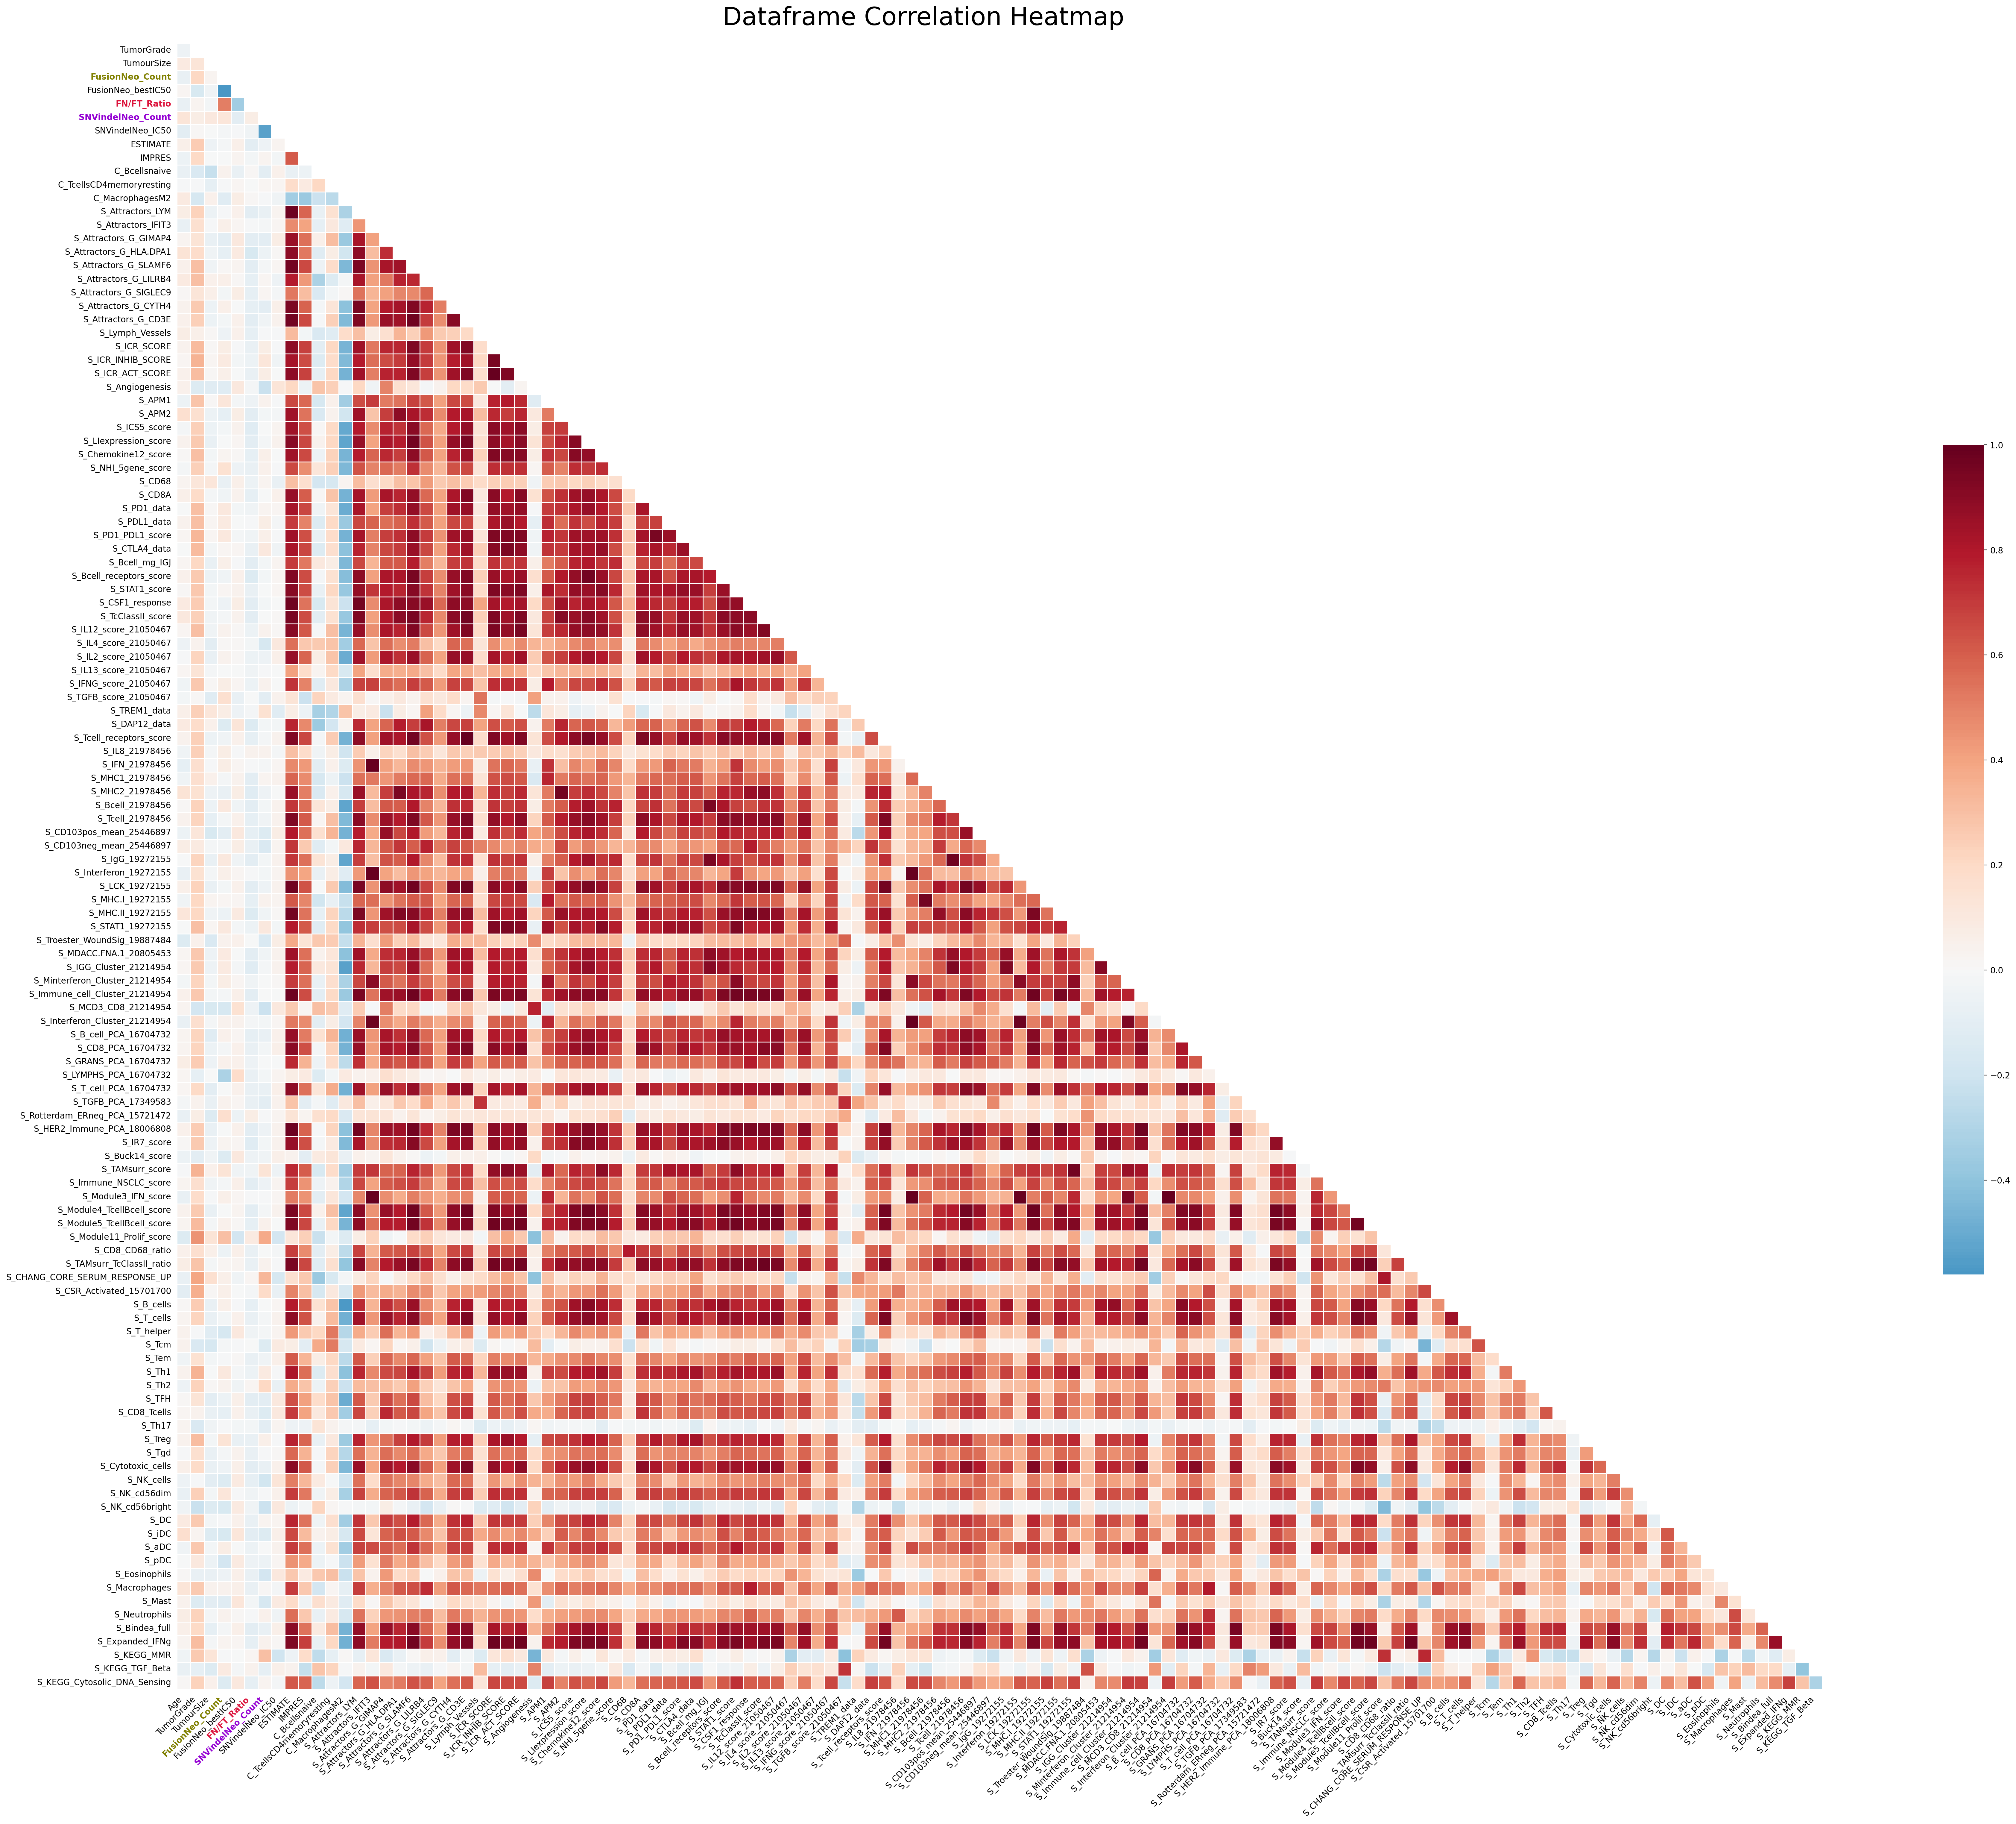
\includegraphics[width=35.08333in,height=31.73958in]{xgboost_tuned_files/figure-pdf/cell-22-output-1.png}

Now, draw the same on the subset Y labels grouped as
\texttt{activator\_T}.

\begin{Shaded}
\begin{Highlighting}[]
\CommentTok{\# get the list from the dict}
\NormalTok{activator\_t }\OperatorTok{=}\NormalTok{ imscore\_series\_dict[}\StringTok{\textquotesingle{}activator\_T\textquotesingle{}}\NormalTok{]}
\NormalTok{suppressor\_t }\OperatorTok{=}\NormalTok{ imscore\_series\_dict[}\StringTok{\textquotesingle{}suppressor\_T\textquotesingle{}}\NormalTok{]}
\NormalTok{best\_prog }\OperatorTok{=}\NormalTok{ imscore\_series\_dict[}\StringTok{\textquotesingle{}HR\textless{}1\_best\_10\_prog\textquotesingle{}}\NormalTok{]}
\NormalTok{worst\_prog }\OperatorTok{=}\NormalTok{ imscore\_series\_dict[}\StringTok{\textquotesingle{}HR\textgreater{}1\_worst\_10\_prog\textquotesingle{}}\NormalTok{]}

\CommentTok{\# combine these with the X feature set (unique only using set())}
\NormalTok{merged\_cols }\OperatorTok{=}\NormalTok{ X\_features\_nocat }\OperatorTok{+}\NormalTok{ activator\_t }\OperatorTok{+}\NormalTok{ suppressor\_t }\OperatorTok{+}\NormalTok{ best\_prog }\OperatorTok{+}\NormalTok{ worst\_prog}
\NormalTok{merged\_cols }\OperatorTok{=} \BuiltInTok{list}\NormalTok{(}\BuiltInTok{set}\NormalTok{(merged\_cols))}
\BuiltInTok{print}\NormalTok{(}\SpecialStringTok{f"Total number of elements in merged\_cols (unsorted): }\SpecialCharTok{\{}\BuiltInTok{len}\NormalTok{(merged\_cols)}\SpecialCharTok{\}}\SpecialStringTok{"}\NormalTok{)}

\CommentTok{\# there are repeated immune scores (at least in between two groups, can be more than two groups) so get a list of them first}
\ImportTok{from}\NormalTok{ itertools }\ImportTok{import}\NormalTok{ combinations}
\CommentTok{\# list of all the sets}
\NormalTok{all\_sets }\OperatorTok{=}\NormalTok{ [}\BuiltInTok{set}\NormalTok{(activator\_t), }\BuiltInTok{set}\NormalTok{(suppressor\_t), }\BuiltInTok{set}\NormalTok{(best\_prog), }\BuiltInTok{set}\NormalTok{(worst\_prog)]}

\CommentTok{\# Get all possible combinations of 2 sets}
\NormalTok{set\_combo }\OperatorTok{=}\NormalTok{ combinations(all\_sets, }\DecValTok{2}\NormalTok{)}

\CommentTok{\# Find the union of all set combinations}
\NormalTok{union\_of\_combo }\OperatorTok{=} \BuiltInTok{list}\NormalTok{(}\BuiltInTok{set}\NormalTok{.union(}\OperatorTok{*}\NormalTok{[}\BuiltInTok{set}\NormalTok{.intersection(c1, c2) }\ControlFlowTok{for}\NormalTok{ c1, c2 }\KeywordTok{in}\NormalTok{ set\_combo]))}

\BuiltInTok{print}\NormalTok{(}\SpecialStringTok{f"Elements that overlap between at least two sets: }\SpecialCharTok{\{}\NormalTok{union\_of\_combo}\SpecialCharTok{\}}\SpecialStringTok{"}\NormalTok{)}

\CommentTok{\# rearrange the list element order based on another list}
\NormalTok{merged\_cols }\OperatorTok{=}\NormalTok{ [x }\ControlFlowTok{for}\NormalTok{ x }\KeywordTok{in}\NormalTok{ X\_features\_nocat] }\OperatorTok{+}\NormalTok{ union\_of\_combo }\OperatorTok{+}\NormalTok{ [x }\ControlFlowTok{for}\NormalTok{ x }\KeywordTok{in}\NormalTok{ activator\_t }\ControlFlowTok{if}\NormalTok{ x }\KeywordTok{not} \KeywordTok{in}\NormalTok{ union\_of\_combo] }\OperatorTok{+}\NormalTok{ [x }\ControlFlowTok{for}\NormalTok{ x }\KeywordTok{in}\NormalTok{ suppressor\_t }\ControlFlowTok{if}\NormalTok{ x }\KeywordTok{not} \KeywordTok{in}\NormalTok{ union\_of\_combo] }\OperatorTok{+}\NormalTok{ [x }\ControlFlowTok{for}\NormalTok{ x }\KeywordTok{in}\NormalTok{ best\_prog }\ControlFlowTok{if}\NormalTok{ x }\KeywordTok{not} \KeywordTok{in}\NormalTok{ union\_of\_combo] }\OperatorTok{+}\NormalTok{ [x }\ControlFlowTok{for}\NormalTok{ x }\KeywordTok{in}\NormalTok{ worst\_prog }\ControlFlowTok{if}\NormalTok{ x }\KeywordTok{not} \KeywordTok{in}\NormalTok{ union\_of\_combo]}

\BuiltInTok{print}\NormalTok{(}\SpecialStringTok{f"Total number of elements in merged\_cols (sorted by original X feature order and groups): }\SpecialCharTok{\{}\BuiltInTok{len}\NormalTok{(merged\_cols)}\SpecialCharTok{\}}\SpecialStringTok{"}\NormalTok{)}
\end{Highlighting}
\end{Shaded}

\begin{verbatim}
Total number of elements in merged_cols (unsorted): 53
Elements that overlap between at least two sets: ['S_TFH', 'S_T_helper', 'S_TGFB_score_21050467', 'S_TGFB_PCA_17349583']
Total number of elements in merged_cols (sorted by original X feature order and groups): 53
\end{verbatim}

\begin{Shaded}
\begin{Highlighting}[]
\CommentTok{\# now subset the dcat data}
\NormalTok{df\_dcat\_ss }\OperatorTok{=}\NormalTok{ df\_dcat[merged\_cols]}
\NormalTok{df\_dcat\_ss.head()}
\end{Highlighting}
\end{Shaded}

\begin{longtable}[]{@{}llllllllllllllllllllllllllllllllllllllllllllllllllllll@{}}
\toprule\noalign{}
& Age & TumorGrade & TumourSize & FusionNeo\_Count & FusionNeo\_bestIC50
& FN/FT\_Ratio & SNVindelNeo\_Count & SNVindelNeo\_IC50 & S\_TFH &
S\_T\_helper & S\_TGFB\_score\_21050467 & S\_TGFB\_PCA\_17349583 &
S\_T\_cells & S\_Tcell\_receptors\_score & S\_Tcell\_21978456 &
S\_CD8\_Tcells & S\_CD8A & S\_Th17 & S\_Tcm & S\_Tem & S\_Th1 &
S\_Cytotoxic\_cells & C\_TcellsCD4memoryresting &
S\_T\_cell\_PCA\_16704732 & S\_Attractors\_G\_CD3E & S\_Tgd &
S\_CD8\_PCA\_16704732 & S\_Module4\_TcellBcell\_score &
S\_Module5\_TcellBcell\_score & S\_CD8\_CD68\_ratio & S\_ICR\_SCORE &
S\_ICR\_ACT\_SCORE & S\_GRANS\_PCA\_16704732 & S\_Treg & S\_CTLA4\_data
& S\_PD1\_data & S\_PDL1\_data & S\_PD1\_PDL1\_score &
S\_IL4\_score\_21050467 & S\_IL13\_score\_21050467 & S\_TcClassII\_score
& S\_KEGG\_TGF\_Beta & S\_ICR\_INHIB\_SCORE & S\_Buck14\_score &
S\_Bcell\_receptors\_score & S\_CD103pos\_mean\_25446897 &
S\_Attractors\_G\_SLAMF6 & S\_ICS5\_score & S\_Lymph\_Vessels &
S\_Rotterdam\_ERneg\_PCA\_15721472 & S\_IFNG\_score\_21050467 &
S\_Module11\_Prolif\_score & S\_TREM1\_data \\
ID & & & & & & & & & & & & & & & & & & & & & & & & & & & & & & & & & & &
& & & & & & & & & & & & & & & & & & \\
\midrule\noalign{}
\endhead
\bottomrule\noalign{}
\endlastfoot
SD0012 & 50 & 2 & 2.3 & 20 & 5.79 & 0.476190 & 357 & 1.7 & 0.3112 &
0.4132 & 0.4403 & 0.4648 & 0.2395 & 0.2526 & 0.2516 & 0.3645 & 0.2942 &
0.2810 & 0.3633 & 0.3210 & 0.2599 & 0.2188 & 0.117468 & 0.3451 & 0.2765
& 0.1945 & 0.2215 & 0.2546 & 0.2730 & 0.2268 & 0.2463 & 0.2495 & 0.3614
& 0.2348 & 0.2061 & 0.1536 & 0.2530 & 0.2042 & 0.3797 & 0.3197 & 0.3435
& 0.3537 & 0.2341 & 0.2094 & 0.2764 & 0.2262 & 0.2749 & 0.2130 & 0.3203
& 0.2937 & 0.4008 & 0.3697 & 0.2907 \\
SD0014 & 58 & 2 & 2.5 & 10 & 5.28 & 0.588235 & 85 & 4.1 & 0.3229 &
0.4092 & 0.4496 & 0.4580 & 0.2909 & 0.3290 & 0.3007 & 0.3713 & 0.3644 &
0.2645 & 0.3404 & 0.3530 & 0.2808 & 0.2985 & 0.207531 & 0.3555 & 0.3525
& 0.1977 & 0.2761 & 0.3111 & 0.3159 & 0.2395 & 0.3051 & 0.3143 & 0.3637
& 0.3182 & 0.2513 & 0.2726 & 0.2377 & 0.2553 & 0.4051 & 0.3308 & 0.3868
& 0.3470 & 0.2701 & 0.2157 & 0.3079 & 0.2859 & 0.3343 & 0.3002 & 0.3452
& 0.3266 & 0.4120 & 0.3126 & 0.2012 \\
SD0015 & 46 & 2 & 1.8 & 4 & 11.48 & 0.250000 & 150 & 2.4 & 0.3225 &
0.4159 & 0.4391 & 0.4442 & 0.2873 & 0.2886 & 0.2830 & 0.3762 & 0.3122 &
0.2370 & 0.3520 & 0.3560 & 0.2600 & 0.2720 & 0.235337 & 0.3489 & 0.3025
& 0.2021 & 0.2671 & 0.2851 & 0.2897 & 0.0936 & 0.2622 & 0.2706 & 0.3591
& 0.2251 & 0.2004 & 0.1932 & 0.2485 & 0.2211 & 0.4038 & 0.3158 & 0.3483
& 0.3522 & 0.2304 & 0.2609 & 0.3040 & 0.2712 & 0.3015 & 0.3055 & 0.3124
& 0.2985 & 0.3986 & 0.2984 & 0.1509 \\
SD0017 & 54 & 2 & 2.5 & 19 & 15.11 & 0.404255 & 1369 & 1.7 & 0.3525 &
0.4170 & 0.4248 & 0.4439 & 0.3460 & 0.3797 & 0.3693 & 0.3879 & 0.4006 &
0.2212 & 0.3275 & 0.3432 & 0.2914 & 0.3151 & 0.148387 & 0.3648 & 0.3957
& 0.2251 & 0.3174 & 0.3576 & 0.3706 & 0.2758 & 0.3589 & 0.3654 & 0.3679
& 0.3330 & 0.2922 & 0.3023 & 0.3429 & 0.3228 & 0.4092 & 0.3338 & 0.4082
& 0.3468 & 0.3341 & 0.2489 & 0.3671 & 0.3003 & 0.3912 & 0.3533 & 0.3131
& 0.2886 & 0.4190 & 0.3377 & 0.1319 \\
SD0018 & 58 & 3 & 3.0 & 39 & 3.00 & 0.309524 & 382 & 1.6 & 0.3041 &
0.3955 & 0.4343 & 0.4654 & 0.2530 & 0.2799 & 0.2670 & 0.3523 & 0.2786 &
0.2401 & 0.3185 & 0.3066 & 0.2713 & 0.2636 & 0.133531 & 0.3393 & 0.3017
& 0.1413 & 0.2308 & 0.2758 & 0.3050 & 0.2009 & 0.2870 & 0.2955 & 0.3603
& 0.2709 & 0.2310 & 0.2363 & 0.2357 & 0.2360 & 0.3689 & 0.3172 & 0.3709
& 0.3444 & 0.2544 & 0.2237 & 0.3054 & 0.2429 & 0.3141 & 0.2892 & 0.3358
& 0.2920 & 0.4095 & 0.3770 & 0.2824 \\
\end{longtable}

\begin{Shaded}
\begin{Highlighting}[]
\CommentTok{\# replot heatmap on transformed data}
\NormalTok{corr\_df }\OperatorTok{=}\NormalTok{ df\_dcat\_ss.corr(method}\OperatorTok{=}\StringTok{\textquotesingle{}spearman\textquotesingle{}}\NormalTok{)}
\NormalTok{corr\_df }\OperatorTok{=}\NormalTok{ corr\_df.}\BuiltInTok{round}\NormalTok{(}\DecValTok{2}\NormalTok{)}

\CommentTok{\# Create a mask for the upper triangle}
\NormalTok{mask }\OperatorTok{=}\NormalTok{ np.triu(np.ones\_like(corr\_df, dtype}\OperatorTok{=}\BuiltInTok{bool}\NormalTok{))}

\NormalTok{plt.figure(figsize}\OperatorTok{=}\NormalTok{(}\DecValTok{46}\NormalTok{, }\DecValTok{36}\NormalTok{))}

\CommentTok{\# Create the correlation matrix and represent it as a heatmap.}
\NormalTok{hm }\OperatorTok{=}\NormalTok{ sns.heatmap(corr\_df, annot }\OperatorTok{=} \VariableTok{False}\NormalTok{, cmap }\OperatorTok{=} \StringTok{\textquotesingle{}RdBu\_r\textquotesingle{}}\NormalTok{, square }\OperatorTok{=} \VariableTok{True}\NormalTok{, linewidths}\OperatorTok{=}\FloatTok{0.5}\NormalTok{, center}\OperatorTok{=}\DecValTok{0}\NormalTok{, mask}\OperatorTok{=}\NormalTok{mask, cbar\_kws}\OperatorTok{=}\NormalTok{\{}\StringTok{"shrink"}\NormalTok{: }\FloatTok{.5}\NormalTok{\})}

\CommentTok{\# Get current labels}
\NormalTok{ylabels }\OperatorTok{=}\NormalTok{ hm.get\_yticklabels()}
\NormalTok{xlabels }\OperatorTok{=}\NormalTok{ hm.get\_xticklabels()}

\CommentTok{\# Hide the first y{-}axis label and the last x{-}axis label}
\NormalTok{ylabels[}\DecValTok{0}\NormalTok{].set\_visible(}\VariableTok{False}\NormalTok{)}
\NormalTok{xlabels[}\OperatorTok{{-}}\DecValTok{1}\NormalTok{].set\_visible(}\VariableTok{False}\NormalTok{)}

\CommentTok{\# Rotate and align the tick labels}
\NormalTok{plt.setp(xlabels, rotation}\OperatorTok{=}\DecValTok{45}\NormalTok{, ha}\OperatorTok{=}\StringTok{\textquotesingle{}right\textquotesingle{}}\NormalTok{)}

\CommentTok{\# Define columns to highlight and their colors}
\NormalTok{highlight\_cols }\OperatorTok{=}\NormalTok{ \{}
    \StringTok{"FN/FT\_Ratio"}\NormalTok{: }\StringTok{"crimson"}\NormalTok{,}
    \StringTok{"FusionNeo\_Count"}\NormalTok{: }\StringTok{"olive"}\NormalTok{,}
    \StringTok{"SNVindelNeo\_Count"}\NormalTok{: }\StringTok{"darkviolet"}
\NormalTok{\}}

\CommentTok{\# Change color of specific x{-}axis and y{-}axis labels}
\ControlFlowTok{for}\NormalTok{ label }\KeywordTok{in}\NormalTok{ xlabels:}
    \ControlFlowTok{if}\NormalTok{ label.get\_text() }\KeywordTok{in}\NormalTok{ highlight\_cols:}
\NormalTok{        label.set\_color(highlight\_cols[label.get\_text()])}
\NormalTok{        label.set\_fontweight(}\StringTok{\textquotesingle{}bold\textquotesingle{}}\NormalTok{)}

\ControlFlowTok{for}\NormalTok{ label }\KeywordTok{in}\NormalTok{ ylabels:}
    \ControlFlowTok{if}\NormalTok{ label.get\_text() }\KeywordTok{in}\NormalTok{ highlight\_cols:}
\NormalTok{        label.set\_color(highlight\_cols[label.get\_text()])}
\NormalTok{        label.set\_fontweight(}\StringTok{\textquotesingle{}bold\textquotesingle{}}\NormalTok{)}

\CommentTok{\# Removes all ticks}
\NormalTok{hm.tick\_params(left}\OperatorTok{=}\VariableTok{False}\NormalTok{, bottom}\OperatorTok{=}\VariableTok{False}\NormalTok{)}

\NormalTok{hm.set\_title(}\StringTok{\textquotesingle{}Dataframe Correlation Heatmap\textquotesingle{}}\NormalTok{, fontsize}\OperatorTok{=}\DecValTok{30}\NormalTok{, x}\OperatorTok{=}\FloatTok{0.45}\NormalTok{)}

\NormalTok{plt.show()}
\end{Highlighting}
\end{Shaded}

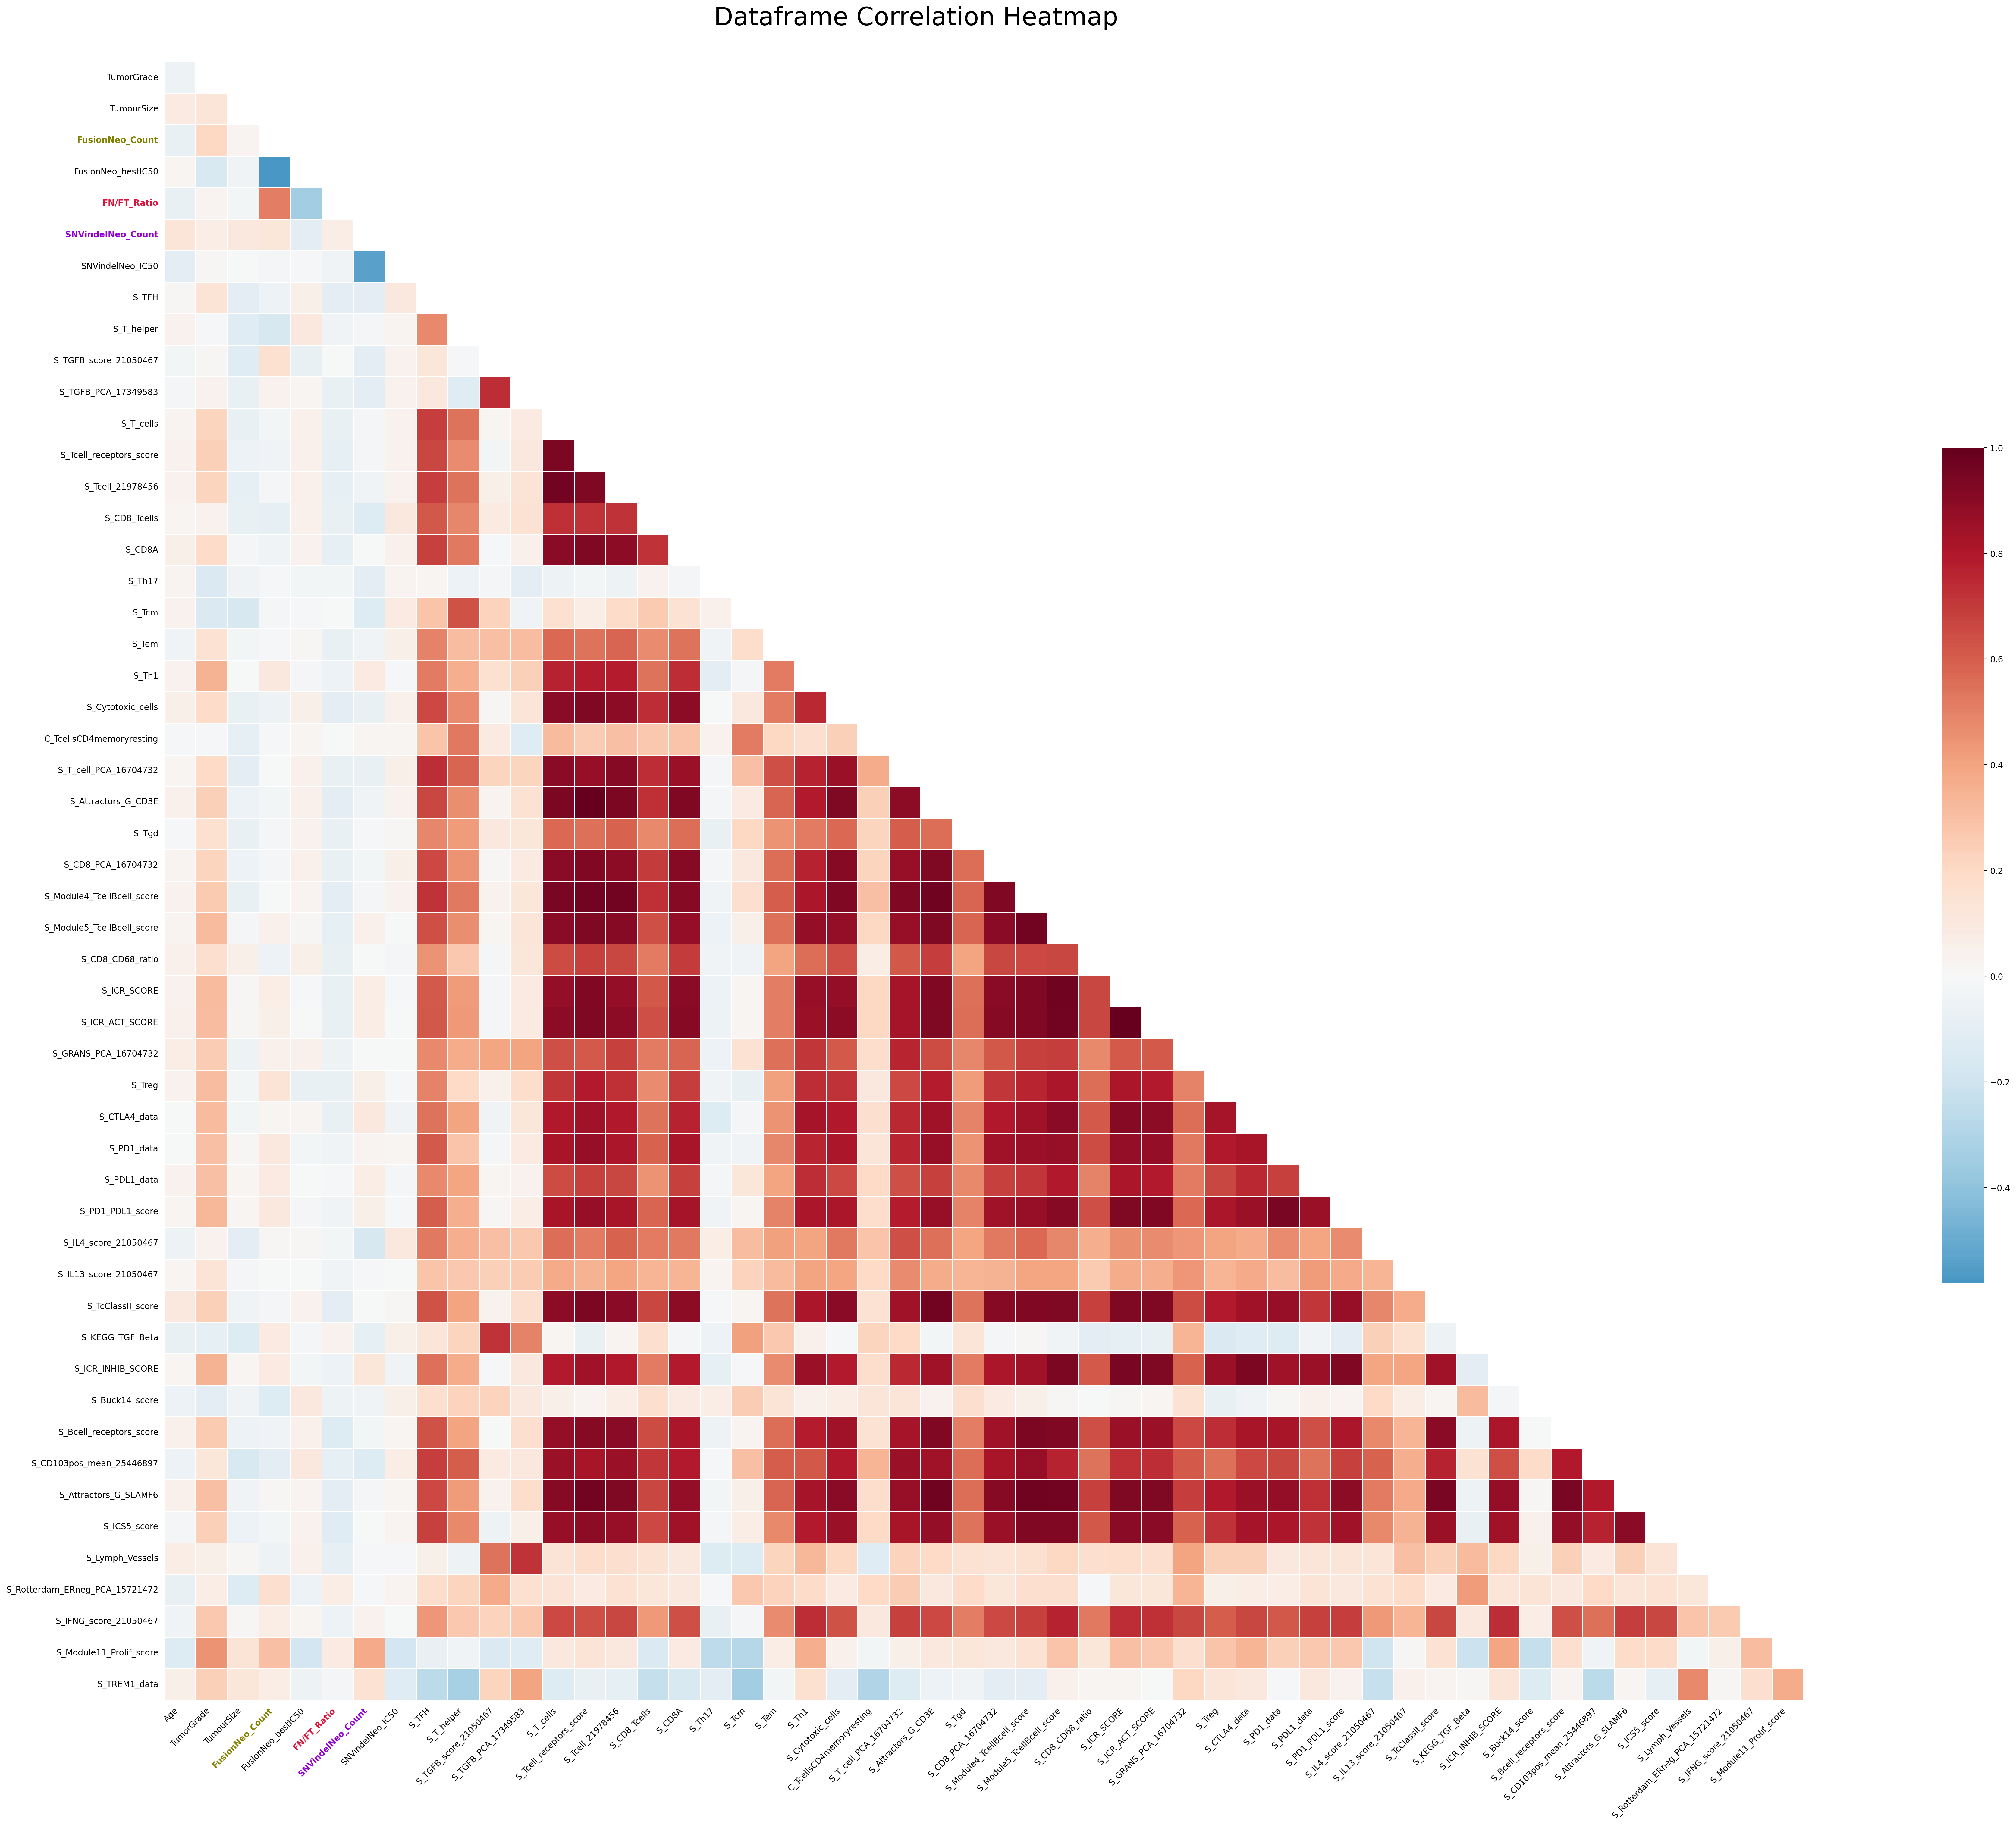
\includegraphics[width=34.84375in,height=31.5625in]{xgboost_tuned_files/figure-pdf/cell-25-output-1.png}

\paragraph{\texorpdfstring{\textbf{Split Dataset with
\texttt{train\_test\_split}}}{Split Dataset with train\_test\_split}}\label{split-dataset-with-train_test_split}

Split the dataset before modeling to avoid information leakage, then
preprocess the data through the set up Pipeline before XGBoost.

\begin{Shaded}
\begin{Highlighting}[]
\CommentTok{\# subset X features; use the list generated before}
\NormalTok{X }\OperatorTok{=}\NormalTok{ dfenc[X\_features]}
\NormalTok{X}
\end{Highlighting}
\end{Shaded}

\begin{longtable}[]{@{}lllllllllllll@{}}
\toprule\noalign{}
& Subtype\_HR+/HER2- & Subtype\_HR+/HER2+ & Subtype\_TNBC &
Subtype\_HR-/HER2+ & Age & TumorGrade & TumourSize & FusionNeo\_Count &
FusionNeo\_bestIC50 & FN/FT\_Ratio & SNVindelNeo\_Count &
SNVindelNeo\_IC50 \\
ID & & & & & & & & & & & & \\
\midrule\noalign{}
\endhead
\bottomrule\noalign{}
\endlastfoot
SD0012 & 1 & 0 & 0 & 0 & 50 & 2 & 2.3 & 20 & 5.79 & 0.476190 & 357 &
1.7 \\
SD0014 & 1 & 0 & 0 & 0 & 58 & 2 & 2.5 & 10 & 5.28 & 0.588235 & 85 &
4.1 \\
SD0015 & 1 & 0 & 0 & 0 & 46 & 2 & 1.8 & 4 & 11.48 & 0.250000 & 150 &
2.4 \\
SD0017 & 1 & 0 & 0 & 0 & 54 & 2 & 2.5 & 19 & 15.11 & 0.404255 & 1369 &
1.7 \\
... & ... & ... & ... & ... & ... & ... & ... & ... & ... & ... & ... &
... \\
SD2406 & 1 & 0 & 0 & 0 & 72 & 2 & 3.0 & 13 & 9.51 & 0.393939 & 512 &
1.8 \\
SD2409 & 1 & 0 & 0 & 0 & 50 & 2 & 2.0 & 4 & 11.17 & 1.333333 & 26 &
2.6 \\
SD2412 & 1 & 0 & 0 & 0 & 49 & 2 & 3.5 & 12 & 43.78 & 0.230769 & 80 &
5.1 \\
SD2418 & 1 & 0 & 0 & 0 & 74 & 2 & 2.2 & 17 & 17.87 & 0.772727 & 264 &
2.7 \\
\end{longtable}

Now grab the Y targets (do this as a whole, but we will train on each
column individually later).

\begin{Shaded}
\begin{Highlighting}[]
\CommentTok{\# Now get the Y variable set}
\NormalTok{Y }\OperatorTok{=}\NormalTok{ dfenc[Y\_labels\_all]}
\NormalTok{Y}
\end{Highlighting}
\end{Shaded}

\begin{longtable}[]{@{}llllllllllllllllllllllllllllllllllllllllllllllllllllllllllllllllllllllllllllllllllllllllllllllllllllllllllllllllllll@{}}
\toprule\noalign{}
& ESTIMATE & IMPRES & C\_Bcellsnaive & C\_TcellsCD4memoryresting &
C\_MacrophagesM2 & S\_Attractors\_LYM & S\_Attractors\_IFIT3 &
S\_Attractors\_G\_GIMAP4 & S\_Attractors\_G\_HLA.DPA1 &
S\_Attractors\_G\_SLAMF6 & S\_Attractors\_G\_LILRB4 &
S\_Attractors\_G\_SIGLEC9 & S\_Attractors\_G\_CYTH4 &
S\_Attractors\_G\_CD3E & S\_Lymph\_Vessels & S\_ICR\_SCORE &
S\_ICR\_INHIB\_SCORE & S\_ICR\_ACT\_SCORE & S\_Angiogenesis & S\_APM1 &
S\_APM2 & S\_ICS5\_score & S\_LIexpression\_score &
S\_Chemokine12\_score & S\_NHI\_5gene\_score & S\_CD68 & S\_CD8A &
S\_PD1\_data & S\_PDL1\_data & S\_PD1\_PDL1\_score & S\_CTLA4\_data &
S\_Bcell\_mg\_IGJ & S\_Bcell\_receptors\_score & S\_STAT1\_score &
S\_CSF1\_response & S\_TcClassII\_score & S\_IL12\_score\_21050467 &
S\_IL4\_score\_21050467 & S\_IL2\_score\_21050467 &
S\_IL13\_score\_21050467 & S\_IFNG\_score\_21050467 &
S\_TGFB\_score\_21050467 & S\_TREM1\_data & S\_DAP12\_data &
S\_Tcell\_receptors\_score & S\_IL8\_21978456 & S\_IFN\_21978456 &
S\_MHC1\_21978456 & S\_MHC2\_21978456 & S\_Bcell\_21978456 &
S\_Tcell\_21978456 & S\_CD103pos\_mean\_25446897 &
S\_CD103neg\_mean\_25446897 & S\_IgG\_19272155 & S\_Interferon\_19272155
& S\_LCK\_19272155 & S\_MHC.I\_19272155 & S\_MHC.II\_19272155 &
S\_STAT1\_19272155 & S\_Troester\_WoundSig\_19887484 &
S\_MDACC.FNA.1\_20805453 & S\_IGG\_Cluster\_21214954 &
S\_Minterferon\_Cluster\_21214954 & S\_Immune\_cell\_Cluster\_21214954 &
S\_MCD3\_CD8\_21214954 & S\_Interferon\_Cluster\_21214954 &
S\_B\_cell\_PCA\_16704732 & S\_CD8\_PCA\_16704732 &
S\_GRANS\_PCA\_16704732 & S\_LYMPHS\_PCA\_16704732 &
S\_T\_cell\_PCA\_16704732 & S\_TGFB\_PCA\_17349583 &
S\_Rotterdam\_ERneg\_PCA\_15721472 & S\_HER2\_Immune\_PCA\_18006808 &
S\_IR7\_score & S\_Buck14\_score & S\_TAMsurr\_score &
S\_Immune\_NSCLC\_score & S\_Module3\_IFN\_score &
S\_Module4\_TcellBcell\_score & S\_Module5\_TcellBcell\_score &
S\_Module11\_Prolif\_score & S\_CD8\_CD68\_ratio &
S\_TAMsurr\_TcClassII\_ratio & S\_CHANG\_CORE\_SERUM\_RESPONSE\_UP &
S\_CSR\_Activated\_15701700 & S\_B\_cells & S\_T\_cells & S\_T\_helper &
S\_Tcm & S\_Tem & S\_Th1 & S\_Th2 & S\_TFH & S\_CD8\_Tcells & S\_Th17 &
S\_Treg & S\_Tgd & S\_Cytotoxic\_cells & S\_NK\_cells & S\_NK\_cd56dim &
S\_NK\_cd56bright & S\_DC & S\_iDC & S\_aDC & S\_pDC & S\_Eosinophils &
S\_Macrophages & S\_Mast & S\_Neutrophils & S\_Bindea\_full &
S\_Expanded\_IFNg & S\_KEGG\_MMR & S\_KEGG\_TGF\_Beta &
S\_KEGG\_Cytosolic\_DNA\_Sensing \\
ID & & & & & & & & & & & & & & & & & & & & & & & & & & & & & & & & & & &
& & & & & & & & & & & & & & & & & & & & & & & & & & & & & & & & & & & &
& & & & & & & & & & & & & & & & & & & & & & & & & & & & & & & & & & & &
& & & & & & & & \\
\midrule\noalign{}
\endhead
\bottomrule\noalign{}
\endlastfoot
SD0012 & 2895.605487 & 9 & 0.120394 & 0.117468 & 0.448450 & 0.3620 &
0.4216 & 0.3034 & 0.4425 & 0.2749 & 0.2983 & 0.2756 & 0.3121 & 0.2765 &
0.3203 & 0.2463 & 0.2341 & 0.2495 & 0.3571 & 0.4591 & 0.3985 & 0.2130 &
0.2223 & 0.2766 & 0.3573 & 0.1561 & 0.2942 & 0.1536 & 0.2530 & 0.2042 &
0.2061 & 0.1942 & 0.2764 & 0.3327 & 0.3795 & 0.3435 & 0.2846 & 0.3797 &
0.3761 & 0.3197 & 0.4008 & 0.4403 & 0.2907 & 0.4011 & 0.2526 & 0.2237 &
0.4256 & 0.3971 & 0.4477 & 0.1852 & 0.2516 & 0.2262 & 0.3854 & 0.1591 &
0.4462 & 0.2912 & 0.4211 & 0.4502 & 0.3610 & 0.2711 & 0.3414 & 0.2183 &
0.3728 & 0.3512 & 0.3529 & 0.4162 & 0.3612 & 0.2215 & 0.3614 & 0.4294 &
0.3451 & 0.4648 & 0.2937 & 0.3338 & 0.2999 & 0.2094 & 0.2743 & 0.3203 &
0.4136 & 0.2546 & 0.2730 & 0.3697 & 0.2268 & 0.3335 & 0.3959 & 0.4066 &
0.2199 & 0.2395 & 0.4132 & 0.3633 & 0.3210 & 0.2599 & 0.3561 & 0.3112 &
0.3645 & 0.2810 & 0.2348 & 0.1945 & 0.2188 & 0.3281 & 0.0602 & 0.2038 &
0.2445 & 0.3220 & 0.2212 & 0.2866 & 0.3030 & 0.3657 & 0.2499 & 0.2531 &
0.3031 & 0.3097 & 0.4053 & 0.3537 & 0.2530 \\
SD0014 & 4257.831526 & 11 & 0.165023 & 0.207531 & 0.124223 & 0.4126 &
0.3815 & 0.3619 & 0.4760 & 0.3343 & 0.3001 & 0.2769 & 0.3761 & 0.3525 &
0.3452 & 0.3051 & 0.2701 & 0.3143 & 0.3803 & 0.4819 & 0.4125 & 0.3002 &
0.3106 & 0.3646 & 0.3753 & 0.1030 & 0.3644 & 0.2726 & 0.2377 & 0.2553 &
0.2513 & 0.2820 & 0.3079 & 0.3515 & 0.3869 & 0.3868 & 0.3133 & 0.4051 &
0.4031 & 0.3308 & 0.4120 & 0.4496 & 0.2012 & 0.4360 & 0.3290 & 0.2562 &
0.3882 & 0.4310 & 0.4682 & 0.2990 & 0.3007 & 0.2859 & 0.3998 & 0.2225 &
0.4068 & 0.3481 & 0.4494 & 0.4710 & 0.4011 & 0.2840 & 0.3779 & 0.2727 &
0.3831 & 0.3864 & 0.3511 & 0.3983 & 0.3676 & 0.2761 & 0.3637 & 0.4268 &
0.3555 & 0.4580 & 0.3266 & 0.3549 & 0.3763 & 0.2157 & 0.3028 & 0.3278 &
0.3896 & 0.3111 & 0.3159 & 0.3126 & 0.2395 & 0.3747 & 0.3838 & 0.4030 &
0.2731 & 0.2909 & 0.4092 & 0.3404 & 0.3530 & 0.2808 & 0.3102 & 0.3229 &
0.3713 & 0.2645 & 0.3182 & 0.1977 & 0.2985 & 0.3502 & 0.1191 & 0.3316 &
0.2976 & 0.3445 & 0.2403 & 0.3450 & 0.3203 & 0.3484 & 0.2768 & 0.2783 &
0.3200 & 0.3668 & 0.3803 & 0.3470 & 0.2606 \\
SD0015 & 3123.055856 & 8 & 0.162653 & 0.235337 & 0.279972 & 0.3556 &
0.3782 & 0.3363 & 0.4718 & 0.3015 & 0.2659 & 0.2274 & 0.3180 & 0.3025 &
0.3124 & 0.2622 & 0.2304 & 0.2706 & 0.3761 & 0.4613 & 0.3814 & 0.3055 &
0.2764 & 0.3211 & 0.3784 & -0.1955 & 0.3122 & 0.1932 & 0.2485 & 0.2211 &
0.2004 & 0.2478 & 0.3040 & 0.3316 & 0.3646 & 0.3483 & 0.3012 & 0.4038 &
0.3875 & 0.3158 & 0.3986 & 0.4391 & 0.1509 & 0.3958 & 0.2886 & 0.2535 &
0.3764 & 0.4054 & 0.4601 & 0.2509 & 0.2830 & 0.2712 & 0.3801 & 0.1750 &
0.3987 & 0.3063 & 0.4239 & 0.4616 & 0.3587 & 0.2955 & 0.3431 & 0.2278 &
0.3599 & 0.3549 & 0.4011 & 0.3865 & 0.3661 & 0.2671 & 0.3591 & 0.4313 &
0.3489 & 0.4442 & 0.2985 & 0.3383 & 0.3370 & 0.2609 & 0.2706 & 0.3312 &
0.3792 & 0.2851 & 0.2897 & 0.2984 & 0.0936 & 0.3370 & 0.3880 & 0.4038 &
0.2799 & 0.2873 & 0.4159 & 0.3520 & 0.3560 & 0.2600 & 0.3116 & 0.3225 &
0.3762 & 0.2370 & 0.2251 & 0.2021 & 0.2720 & 0.3434 & 0.0626 & 0.3025 &
0.2670 & 0.3212 & 0.2098 & 0.2967 & 0.3236 & 0.3266 & 0.2455 & 0.2522 &
0.3107 & 0.3372 & 0.3793 & 0.3522 & 0.2564 \\
SD0017 & 5275.497847 & 11 & 0.155523 & 0.148387 & 0.128777 & 0.4314 &
0.4482 & 0.4080 & 0.4980 & 0.3912 & 0.3120 & 0.2934 & 0.3864 & 0.3957 &
0.3131 & 0.3589 & 0.3341 & 0.3654 & 0.3842 & 0.4957 & 0.4328 & 0.3533 &
0.3732 & 0.4177 & 0.4350 & 0.1401 & 0.4006 & 0.3023 & 0.3429 & 0.3228 &
0.2922 & 0.3591 & 0.3671 & 0.3926 & 0.4113 & 0.4082 & 0.3325 & 0.4092 &
0.4129 & 0.3338 & 0.4190 & 0.4248 & 0.1319 & 0.4878 & 0.3797 & 0.1889 &
0.4601 & 0.4445 & 0.4859 & 0.3224 & 0.3693 & 0.3003 & 0.4095 & 0.2938 &
0.4707 & 0.3968 & 0.4616 & 0.4893 & 0.4644 & 0.2735 & 0.3955 & 0.3234 &
0.4165 & 0.4337 & 0.4190 & 0.4511 & 0.3758 & 0.3174 & 0.3679 & 0.4314 &
0.3648 & 0.4439 & 0.2886 & 0.3688 & 0.4143 & 0.2489 & 0.3562 & 0.3498 &
0.4563 & 0.3576 & 0.3706 & 0.3377 & 0.2758 & 0.4006 & 0.4000 & 0.4062 &
0.3182 & 0.3460 & 0.4170 & 0.3275 & 0.3432 & 0.2914 & 0.3307 & 0.3525 &
0.3879 & 0.2212 & 0.3330 & 0.2251 & 0.3151 & 0.3495 & 0.1939 & 0.2953 &
0.3010 & 0.3467 & 0.2547 & 0.3313 & 0.3230 & 0.3597 & 0.2726 & 0.2648 &
0.3309 & 0.4165 & 0.3997 & 0.3468 & 0.2682 \\
... & ... & ... & ... & ... & ... & ... & ... & ... & ... & ... & ... &
... & ... & ... & ... & ... & ... & ... & ... & ... & ... & ... & ... &
... & ... & ... & ... & ... & ... & ... & ... & ... & ... & ... & ... &
... & ... & ... & ... & ... & ... & ... & ... & ... & ... & ... & ... &
... & ... & ... & ... & ... & ... & ... & ... & ... & ... & ... & ... &
... & ... & ... & ... & ... & ... & ... & ... & ... & ... & ... & ... &
... & ... & ... & ... & ... & ... & ... & ... & ... & ... & ... & ... &
... & ... & ... & ... & ... & ... & ... & ... & ... & ... & ... & ... &
... & ... & ... & ... & ... & ... & ... & ... & ... & ... & ... & ... &
... & ... & ... & ... & ... & ... & ... & ... \\
SD2406 & 2758.511524 & 9 & 0.040575 & 0.157374 & 0.372476 & 0.3538 &
0.3675 & 0.3196 & 0.4475 & 0.2878 & 0.2987 & 0.2249 & 0.2977 & 0.2772 &
0.3157 & 0.2587 & 0.2404 & 0.2636 & 0.3613 & 0.4659 & 0.3922 & 0.1966 &
0.2316 & 0.2923 & 0.2813 & 0.1748 & 0.2810 & 0.2205 & 0.2491 & 0.2348 &
0.2304 & 0.0588 & 0.2951 & 0.3204 & 0.3760 & 0.3382 & 0.2889 & 0.3728 &
0.3790 & 0.3174 & 0.3849 & 0.4309 & 0.3109 & 0.4362 & 0.2583 & 0.2269 &
0.3813 & 0.4082 & 0.4513 & 0.0401 & 0.2631 & 0.2357 & 0.3879 & 0.0211 &
0.3995 & 0.2916 & 0.4247 & 0.4515 & 0.3606 & 0.2608 & 0.3098 & 0.1564 &
0.3513 & 0.3567 & 0.3750 & 0.3842 & 0.3501 & 0.2271 & 0.3615 & 0.4321 &
0.3351 & 0.4546 & 0.2928 & 0.3272 & 0.2899 & 0.1731 & 0.2730 & 0.3076 &
0.3788 & 0.2516 & 0.2696 & 0.3959 & 0.2289 & 0.3288 & 0.4173 & 0.4145 &
0.1935 & 0.2306 & 0.4093 & 0.3427 & 0.2848 & 0.2491 & 0.3534 & 0.2957 &
0.3566 & 0.1893 & 0.2477 & -0.0057 & 0.2601 & 0.3146 & 0.0602 & 0.2081 &
0.2756 & 0.3329 & 0.1981 & 0.3020 & 0.3171 & 0.3629 & 0.2257 & 0.2302 &
0.2934 & 0.3086 & 0.4236 & 0.3489 & 0.2568 \\
SD2409 & 5379.451341 & 11 & 0.098933 & 0.065574 & 0.336374 & 0.4315 &
0.4001 & 0.4281 & 0.4980 & 0.3670 & 0.3599 & 0.3109 & 0.3885 & 0.3636 &
0.4058 & 0.3074 & 0.2588 & 0.3201 & 0.4278 & 0.4789 & 0.4486 & 0.2958 &
0.3271 & 0.3578 & 0.4093 & 0.2096 & 0.3742 & 0.2676 & 0.2780 & 0.2728 &
0.2282 & 0.3606 & 0.3481 & 0.3615 & 0.4254 & 0.3986 & 0.3114 & 0.4257 &
0.4138 & 0.3804 & 0.4204 & 0.4438 & 0.2689 & 0.5003 & 0.3371 & 0.3379 &
0.4041 & 0.4373 & 0.4943 & 0.3594 & 0.3169 & 0.3037 & 0.4367 & 0.2960 &
0.4184 & 0.3754 & 0.4485 & 0.4846 & 0.3863 & 0.3134 & 0.4283 & 0.3230 &
0.3787 & 0.4163 & 0.4373 & 0.4103 & 0.3737 & 0.2959 & 0.3780 & 0.4324 &
0.3626 & 0.4790 & 0.3242 & 0.3694 & 0.4018 & 0.1984 & 0.2949 & 0.3494 &
0.3979 & 0.3243 & 0.3352 & 0.2980 & 0.2940 & 0.3837 & 0.3991 & 0.4168 &
0.2902 & 0.3016 & 0.4070 & 0.3236 & 0.3370 & 0.2773 & 0.3046 & 0.3263 &
0.3789 & 0.2107 & 0.2569 & 0.2197 & 0.3364 & 0.3517 & 0.1525 & 0.3144 &
0.3632 & 0.3714 & 0.2620 & 0.4239 & 0.3225 & 0.3916 & 0.3130 & 0.3030 &
0.3316 & 0.3701 & 0.3928 & 0.3509 & 0.2660 \\
SD2412 & 4225.584090 & 10 & 0.173398 & 0.207518 & 0.206046 & 0.4012 &
0.4299 & 0.3902 & 0.4827 & 0.3308 & 0.2883 & 0.2645 & 0.3532 & 0.3307 &
0.3501 & 0.2914 & 0.2594 & 0.2998 & 0.4215 & 0.4689 & 0.4101 & 0.2921 &
0.2960 & 0.3519 & 0.4009 & 0.1197 & 0.3624 & 0.2331 & 0.2785 & 0.2560 &
0.2199 & 0.2859 & 0.3213 & 0.3555 & 0.3963 & 0.3732 & 0.3114 & 0.4212 &
0.4116 & 0.3613 & 0.4112 & 0.4515 & 0.1930 & 0.4146 & 0.3027 & 0.2417 &
0.4171 & 0.4003 & 0.4708 & 0.3035 & 0.3050 & 0.3060 & 0.4193 & 0.2516 &
0.4358 & 0.3525 & 0.4096 & 0.4776 & 0.4012 & 0.3032 & 0.3910 & 0.2762 &
0.3900 & 0.3891 & 0.4143 & 0.4119 & 0.3790 & 0.2756 & 0.3649 & 0.4301 &
0.3595 & 0.4676 & 0.3259 & 0.3577 & 0.3666 & 0.2383 & 0.3118 & 0.3334 &
0.4189 & 0.3155 & 0.3162 & 0.3044 & 0.2460 & 0.3643 & 0.3864 & 0.4062 &
0.2942 & 0.3026 & 0.4215 & 0.3600 & 0.3633 & 0.2781 & 0.3185 & 0.3387 &
0.3711 & 0.2080 & 0.2333 & 0.1697 & 0.2862 & 0.3441 & 0.1187 & 0.2648 &
0.3162 & 0.3431 & 0.2301 & 0.3355 & 0.3413 & 0.3496 & 0.2730 & 0.2748 &
0.3238 & 0.3560 & 0.3815 & 0.3596 & 0.2491 \\
SD2418 & 4774.602798 & 9 & 0.117058 & 0.243782 & 0.277604 & 0.4254 &
0.4221 & 0.3631 & 0.4951 & 0.3487 & 0.3314 & 0.3077 & 0.3607 & 0.3500 &
0.3505 & 0.3235 & 0.2908 & 0.3320 & 0.3746 & 0.4853 & 0.4419 & 0.2960 &
0.3042 & 0.3473 & 0.4130 & 0.1257 & 0.3791 & 0.2575 & 0.2910 & 0.2744 &
0.2594 & 0.3583 & 0.3261 & 0.3722 & 0.4154 & 0.3925 & 0.3258 & 0.4092 &
0.4006 & 0.3251 & 0.4131 & 0.4466 & 0.2654 & 0.4736 & 0.3285 & 0.1966 &
0.4315 & 0.4426 & 0.4951 & 0.3212 & 0.3321 & 0.2835 & 0.4145 & 0.2408 &
0.4493 & 0.3538 & 0.4528 & 0.4865 & 0.4305 & 0.2833 & 0.4032 & 0.3058 &
0.3931 & 0.4101 & 0.3594 & 0.4195 & 0.3746 & 0.2839 & 0.3682 & 0.4237 &
0.3598 & 0.4645 & 0.3018 & 0.3602 & 0.3782 & 0.2253 & 0.3274 & 0.3475 &
0.4265 & 0.3162 & 0.3365 & 0.3433 & 0.2577 & 0.3831 & 0.3977 & 0.4108 &
0.2873 & 0.3153 & 0.4120 & 0.3498 & 0.3359 & 0.2841 & 0.3405 & 0.3247 &
0.3672 & 0.2736 & 0.3118 & 0.1389 & 0.2862 & 0.3378 & 0.0954 & 0.1935 &
0.2901 & 0.3575 & 0.2500 & 0.3003 & 0.3100 & 0.3676 & 0.2489 & 0.2636 &
0.3191 & 0.3735 & 0.4077 & 0.3418 & 0.2582 \\
\end{longtable}

Now we perform train test split on the X and Y variables.

\begin{Shaded}
\begin{Highlighting}[]
\CommentTok{\# Perform train{-}test split}
\ImportTok{from}\NormalTok{ sklearn.model\_selection }\ImportTok{import}\NormalTok{ train\_test\_split}
\NormalTok{X\_train, X\_test, Y\_train, Y\_test }\OperatorTok{=}\NormalTok{ train\_test\_split(X, Y, test\_size}\OperatorTok{=}\FloatTok{0.2}\NormalTok{, random\_state}\OperatorTok{=}\DecValTok{42}\NormalTok{)}
\end{Highlighting}
\end{Shaded}

As we don't want to transform all the X columns (because some of them
are discrete numerical data and some of them are one-hot encoded
categorical variables), we need to specify the columns to transform.

\paragraph{\texorpdfstring{\textbf{Create a Data Transformation Pipeline
from \texttt{feature\_engine}
Package}}{Create a Data Transformation Pipeline from feature\_engine Package}}\label{create-a-data-transformation-pipeline-from-feature_engine-package}

First, the pipeline will apply the Yeo-Johnson transformation on the
split datasets on select X features and all Y labels, and scale them
using \texttt{StandardScaler} (but wrapped within
\texttt{feature\_engine}'s wrapper) on select X features and all Y
labels.

This pipeline would enable easy inverse transform steps for both X and Y
datasets later.

\begin{Shaded}
\begin{Highlighting}[]
\NormalTok{X\_vars\_to\_transform }\OperatorTok{=}\NormalTok{ [}\StringTok{\textquotesingle{}TumourSize\textquotesingle{}}\NormalTok{, }\StringTok{\textquotesingle{}FusionNeo\_Count\textquotesingle{}}\NormalTok{, }\StringTok{\textquotesingle{}FusionNeo\_bestIC50\textquotesingle{}}\NormalTok{, }\StringTok{\textquotesingle{}FN/FT\_Ratio\textquotesingle{}}\NormalTok{, }\StringTok{\textquotesingle{}SNVindelNeo\_Count\textquotesingle{}}\NormalTok{, }\StringTok{\textquotesingle{}SNVindelNeo\_IC50\textquotesingle{}}\NormalTok{]}
\end{Highlighting}
\end{Shaded}

Do for X datasets.

\begin{Shaded}
\begin{Highlighting}[]
\ImportTok{from}\NormalTok{ feature\_engine.pipeline }\ImportTok{import}\NormalTok{ Pipeline}
\ImportTok{from}\NormalTok{ feature\_engine.transformation }\ImportTok{import}\NormalTok{ YeoJohnsonTransformer}
\ImportTok{from}\NormalTok{ feature\_engine.wrappers }\ImportTok{import}\NormalTok{ SklearnTransformerWrapper}
\ImportTok{from}\NormalTok{ sklearn.preprocessing }\ImportTok{import}\NormalTok{ StandardScaler}

\CommentTok{\# select variables to scale}
\NormalTok{scale\_cols\_X }\OperatorTok{=}\NormalTok{ X\_train.columns.tolist()}
\NormalTok{scale\_cols\_X }\OperatorTok{=}\NormalTok{ [col }\ControlFlowTok{for}\NormalTok{ col }\KeywordTok{in}\NormalTok{ scale\_cols\_X }\ControlFlowTok{if}\NormalTok{ col }\KeywordTok{not} \KeywordTok{in}\NormalTok{ [}\StringTok{\textquotesingle{}Age\textquotesingle{}}\NormalTok{, }\StringTok{\textquotesingle{}TumorGrade\textquotesingle{}}\NormalTok{, }\StringTok{\textquotesingle{}Subtype\_HR+/HER2{-}\textquotesingle{}}\NormalTok{, }\StringTok{\textquotesingle{}Subtype\_HR+/HER2+\textquotesingle{}}\NormalTok{, }\StringTok{\textquotesingle{}Subtype\_TNBC\textquotesingle{}}\NormalTok{, }\StringTok{\textquotesingle{}Subtype\_HR{-}/HER2+\textquotesingle{}}\NormalTok{]]}

\CommentTok{\# Create the pipeline}
\NormalTok{preprocess\_pipeline\_X }\OperatorTok{=}\NormalTok{ Pipeline([}
\NormalTok{    (}\StringTok{\textquotesingle{}yeo\_johnson\textquotesingle{}}\NormalTok{, YeoJohnsonTransformer(variables}\OperatorTok{=}\NormalTok{X\_vars\_to\_transform)),}
\NormalTok{    (}\StringTok{\textquotesingle{}scaler\textquotesingle{}}\NormalTok{, SklearnTransformerWrapper(transformer }\OperatorTok{=}\NormalTok{ StandardScaler(), variables }\OperatorTok{=}\NormalTok{ scale\_cols\_X))}
\NormalTok{])}

\CommentTok{\# Fit the pipeline to the training data}
\NormalTok{preprocess\_pipeline\_X.fit(X\_train)}

\CommentTok{\# Transform the training data}
\NormalTok{X\_train\_yjs }\OperatorTok{=}\NormalTok{ preprocess\_pipeline\_X.transform(X\_train)}
\CommentTok{\# Transform the test data}
\NormalTok{X\_test\_yjs }\OperatorTok{=}\NormalTok{ preprocess\_pipeline\_X.transform(X\_test)}
\end{Highlighting}
\end{Shaded}

\begin{Shaded}
\begin{Highlighting}[]
\NormalTok{X\_train}
\end{Highlighting}
\end{Shaded}

\begin{longtable}[]{@{}lllllllllllll@{}}
\toprule\noalign{}
& Subtype\_HR+/HER2- & Subtype\_HR+/HER2+ & Subtype\_TNBC &
Subtype\_HR-/HER2+ & Age & TumorGrade & TumourSize & FusionNeo\_Count &
FusionNeo\_bestIC50 & FN/FT\_Ratio & SNVindelNeo\_Count &
SNVindelNeo\_IC50 \\
ID & & & & & & & & & & & & \\
\midrule\noalign{}
\endhead
\bottomrule\noalign{}
\endlastfoot
SD0907 & 0 & 0 & 0 & 1 & 64 & 2 & 2.5 & 47 & 4.86 & 0.580247 & 177 &
3.2 \\
SD0850 & 1 & 0 & 0 & 0 & 50 & 3 & 2.0 & 20 & 9.90 & 0.392157 & 362 &
1.7 \\
SD0050 & 0 & 1 & 0 & 0 & 45 & 3 & 4.0 & 37 & 6.92 & 0.536232 & 317 &
1.6 \\
SD1753 & 1 & 0 & 0 & 0 & 73 & 2 & 3.0 & 1 & 454.07 & 0.166667 & 63 &
2.7 \\
... & ... & ... & ... & ... & ... & ... & ... & ... & ... & ... & ... &
... \\
SD0339 & 0 & 0 & 0 & 1 & 66 & 3 & 3.5 & 117 & 5.52 & 0.587940 & 284 &
1.3 \\
SD0994 & 0 & 1 & 0 & 0 & 64 & 3 & 3.5 & 6 & 9.41 & 0.171429 & 138 &
2.0 \\
SD1532 & 1 & 0 & 0 & 0 & 67 & 2 & 2.5 & 55 & 2.43 & 0.591398 & 543 &
2.2 \\
SD0326 & 0 & 0 & 0 & 1 & 43 & 2 & 5.0 & 74 & 5.20 & 0.755102 & 196 &
2.8 \\
\end{longtable}

\begin{Shaded}
\begin{Highlighting}[]
\NormalTok{X\_train\_yjs}
\end{Highlighting}
\end{Shaded}

\begin{longtable}[]{@{}lllllllllllll@{}}
\toprule\noalign{}
& Subtype\_HR+/HER2- & Subtype\_HR+/HER2+ & Subtype\_TNBC &
Subtype\_HR-/HER2+ & Age & TumorGrade & TumourSize & FusionNeo\_Count &
FusionNeo\_bestIC50 & FN/FT\_Ratio & SNVindelNeo\_Count &
SNVindelNeo\_IC50 \\
ID & & & & & & & & & & & & \\
\midrule\noalign{}
\endhead
\bottomrule\noalign{}
\endlastfoot
SD0907 & 0 & 0 & 0 & 1 & 64 & 2 & -0.198167 & 1.084700 & -0.561304 &
0.536308 & -0.569045 & 1.016003 \\
SD0850 & 1 & 0 & 0 & 0 & 50 & 3 & -0.674861 & 0.115984 & 0.408689 &
-0.373761 & 0.088991 & -0.672361 \\
SD0050 & 0 & 1 & 0 & 0 & 45 & 3 & 0.755274 & 0.801083 & -0.045619 &
0.339224 & -0.030124 & -0.887022 \\
SD1753 & 1 & 0 & 0 & 0 & 73 & 2 & 0.181899 & -2.165375 & 2.337760 &
-1.760274 & -1.588698 & 0.657471 \\
... & ... & ... & ... & ... & ... & ... & ... & ... & ... & ... & ... &
... \\
SD0339 & 0 & 0 & 0 & 1 & 66 & 3 & 0.493716 & 2.254499 & -0.367907 &
0.569864 & -0.129784 & -1.691642 \\
SD0994 & 0 & 1 & 0 & 0 & 64 & 3 & 0.493716 & -1.030586 & 0.348478 &
-1.726679 & -0.807226 & -0.143442 \\
SD1532 & 1 & 0 & 0 & 0 & 67 & 2 & -0.198167 & 1.276271 & -1.741884 &
0.584865 & 0.444600 & 0.135236 \\
SD0326 & 0 & 0 & 0 & 1 & 43 & 2 & 1.172027 & 1.649245 & -0.457567 &
1.240736 & -0.472856 & 0.739698 \\
\end{longtable}

\begin{Shaded}
\begin{Highlighting}[]
\CommentTok{\# select variables to scale}
\NormalTok{scale\_cols\_Y }\OperatorTok{=}\NormalTok{ Y\_train.columns.tolist()}

\CommentTok{\# Create the pipeline}
\NormalTok{preprocess\_pipeline\_Y }\OperatorTok{=}\NormalTok{ Pipeline([}
\NormalTok{    (}\StringTok{\textquotesingle{}yeo\_johnson\textquotesingle{}}\NormalTok{, YeoJohnsonTransformer()),}
\NormalTok{    (}\StringTok{\textquotesingle{}scaler\textquotesingle{}}\NormalTok{, SklearnTransformerWrapper(transformer }\OperatorTok{=}\NormalTok{ StandardScaler(), variables }\OperatorTok{=}\NormalTok{ scale\_cols\_Y))}
\NormalTok{])}

\CommentTok{\# Fit the pipeline to the training data}
\NormalTok{preprocess\_pipeline\_Y.fit(Y\_train)}

\CommentTok{\# Transform the training data}
\NormalTok{Y\_train\_yjs }\OperatorTok{=}\NormalTok{ preprocess\_pipeline\_Y.transform(Y\_train)}
\CommentTok{\# Transform the test data}
\NormalTok{Y\_test\_yjs }\OperatorTok{=}\NormalTok{ preprocess\_pipeline\_Y.transform(Y\_test)}
\end{Highlighting}
\end{Shaded}

\begin{Shaded}
\begin{Highlighting}[]
\NormalTok{Y\_train}
\end{Highlighting}
\end{Shaded}

\begin{longtable}[]{@{}llllllllllllllllllllllllllllllllllllllllllllllllllllllllllllllllllllllllllllllllllllllllllllllllllllllllllllllllllll@{}}
\toprule\noalign{}
& ESTIMATE & IMPRES & C\_Bcellsnaive & C\_TcellsCD4memoryresting &
C\_MacrophagesM2 & S\_Attractors\_LYM & S\_Attractors\_IFIT3 &
S\_Attractors\_G\_GIMAP4 & S\_Attractors\_G\_HLA.DPA1 &
S\_Attractors\_G\_SLAMF6 & S\_Attractors\_G\_LILRB4 &
S\_Attractors\_G\_SIGLEC9 & S\_Attractors\_G\_CYTH4 &
S\_Attractors\_G\_CD3E & S\_Lymph\_Vessels & S\_ICR\_SCORE &
S\_ICR\_INHIB\_SCORE & S\_ICR\_ACT\_SCORE & S\_Angiogenesis & S\_APM1 &
S\_APM2 & S\_ICS5\_score & S\_LIexpression\_score &
S\_Chemokine12\_score & S\_NHI\_5gene\_score & S\_CD68 & S\_CD8A &
S\_PD1\_data & S\_PDL1\_data & S\_PD1\_PDL1\_score & S\_CTLA4\_data &
S\_Bcell\_mg\_IGJ & S\_Bcell\_receptors\_score & S\_STAT1\_score &
S\_CSF1\_response & S\_TcClassII\_score & S\_IL12\_score\_21050467 &
S\_IL4\_score\_21050467 & S\_IL2\_score\_21050467 &
S\_IL13\_score\_21050467 & S\_IFNG\_score\_21050467 &
S\_TGFB\_score\_21050467 & S\_TREM1\_data & S\_DAP12\_data &
S\_Tcell\_receptors\_score & S\_IL8\_21978456 & S\_IFN\_21978456 &
S\_MHC1\_21978456 & S\_MHC2\_21978456 & S\_Bcell\_21978456 &
S\_Tcell\_21978456 & S\_CD103pos\_mean\_25446897 &
S\_CD103neg\_mean\_25446897 & S\_IgG\_19272155 & S\_Interferon\_19272155
& S\_LCK\_19272155 & S\_MHC.I\_19272155 & S\_MHC.II\_19272155 &
S\_STAT1\_19272155 & S\_Troester\_WoundSig\_19887484 &
S\_MDACC.FNA.1\_20805453 & S\_IGG\_Cluster\_21214954 &
S\_Minterferon\_Cluster\_21214954 & S\_Immune\_cell\_Cluster\_21214954 &
S\_MCD3\_CD8\_21214954 & S\_Interferon\_Cluster\_21214954 &
S\_B\_cell\_PCA\_16704732 & S\_CD8\_PCA\_16704732 &
S\_GRANS\_PCA\_16704732 & S\_LYMPHS\_PCA\_16704732 &
S\_T\_cell\_PCA\_16704732 & S\_TGFB\_PCA\_17349583 &
S\_Rotterdam\_ERneg\_PCA\_15721472 & S\_HER2\_Immune\_PCA\_18006808 &
S\_IR7\_score & S\_Buck14\_score & S\_TAMsurr\_score &
S\_Immune\_NSCLC\_score & S\_Module3\_IFN\_score &
S\_Module4\_TcellBcell\_score & S\_Module5\_TcellBcell\_score &
S\_Module11\_Prolif\_score & S\_CD8\_CD68\_ratio &
S\_TAMsurr\_TcClassII\_ratio & S\_CHANG\_CORE\_SERUM\_RESPONSE\_UP &
S\_CSR\_Activated\_15701700 & S\_B\_cells & S\_T\_cells & S\_T\_helper &
S\_Tcm & S\_Tem & S\_Th1 & S\_Th2 & S\_TFH & S\_CD8\_Tcells & S\_Th17 &
S\_Treg & S\_Tgd & S\_Cytotoxic\_cells & S\_NK\_cells & S\_NK\_cd56dim &
S\_NK\_cd56bright & S\_DC & S\_iDC & S\_aDC & S\_pDC & S\_Eosinophils &
S\_Macrophages & S\_Mast & S\_Neutrophils & S\_Bindea\_full &
S\_Expanded\_IFNg & S\_KEGG\_MMR & S\_KEGG\_TGF\_Beta &
S\_KEGG\_Cytosolic\_DNA\_Sensing \\
ID & & & & & & & & & & & & & & & & & & & & & & & & & & & & & & & & & & &
& & & & & & & & & & & & & & & & & & & & & & & & & & & & & & & & & & & &
& & & & & & & & & & & & & & & & & & & & & & & & & & & & & & & & & & & &
& & & & & & & & \\
\midrule\noalign{}
\endhead
\bottomrule\noalign{}
\endlastfoot
SD0907 & 5087.085018 & 12 & 0.118125 & 0.256480 & 0.165096 & 0.4142 &
0.4760 & 0.3919 & 0.4921 & 0.3844 & 0.3343 & 0.3073 & 0.3640 & 0.3604 &
0.3475 & 0.3574 & 0.3291 & 0.3648 & 0.3590 & 0.4875 & 0.4452 & 0.3611 &
0.3395 & 0.4598 & 0.4458 & 0.1021 & 0.3835 & 0.2815 & 0.3298 & 0.3058 &
0.2838 & 0.3775 & 0.3519 & 0.3987 & 0.4151 & 0.4071 & 0.3404 & 0.3838 &
0.4119 & 0.3754 & 0.4066 & 0.4280 & 0.2817 & 0.4651 & 0.3490 & 0.2439 &
0.4762 & 0.4304 & 0.4948 & 0.3513 & 0.3549 & 0.2850 & 0.3981 & 0.2854 &
0.4880 & 0.3775 & 0.4485 & 0.4918 & 0.4791 & 0.2630 & 0.4153 & 0.3499 &
0.4350 & 0.4301 & 0.2917 & 0.4557 & 0.3866 & 0.2994 & 0.3660 & 0.4321 &
0.3605 & 0.4424 & 0.2864 & 0.3656 & 0.3989 & 0.2009 & 0.4268 & 0.3502 &
0.4724 & 0.3500 & 0.3830 & 0.3950 & 0.2495 & 0.4101 & 0.4071 & 0.4079 &
0.3258 & 0.3354 & 0.4259 & 0.3548 & 0.3213 & 0.2933 & 0.3484 & 0.3260 &
0.3699 & 0.2996 & 0.2953 & 0.2180 & 0.3140 & 0.3230 & 0.2266 & 0.2121 &
0.3060 & 0.3194 & 0.2668 & 0.3132 & 0.2935 & 0.3684 & 0.2259 & 0.2696 &
0.3235 & 0.4169 & 0.4112 & 0.3337 & 0.2683 \\
SD0850 & 3163.224848 & 8 & 0.103919 & 0.070753 & 0.272750 & 0.3671 &
0.4333 & 0.3166 & 0.4604 & 0.2911 & 0.3122 & 0.2923 & 0.3237 & 0.2783 &
0.3638 & 0.2715 & 0.2473 & 0.2778 & 0.3736 & 0.4796 & 0.4076 & 0.2594 &
0.2585 & 0.3186 & 0.3881 & 0.1263 & 0.2680 & 0.2008 & 0.2537 & 0.2275 &
0.2207 & 0.2605 & 0.2971 & 0.3442 & 0.3749 & 0.3534 & 0.2832 & 0.3780 &
0.3914 & 0.3175 & 0.4106 & 0.4416 & 0.2741 & 0.4535 & 0.2492 & 0.2219 &
0.4382 & 0.4149 & 0.4703 & 0.2862 & 0.2611 & 0.2523 & 0.3920 & 0.2026 &
0.4519 & 0.2968 & 0.4346 & 0.4557 & 0.3906 & 0.2755 & 0.3700 & 0.2613 &
0.3745 & 0.3611 & 0.3533 & 0.4229 & 0.3573 & 0.2310 & 0.3660 & 0.4276 &
0.3390 & 0.4695 & 0.3083 & 0.3412 & 0.3574 & 0.2084 & 0.2990 & 0.3441 &
0.4180 & 0.2639 & 0.2924 & 0.3733 & 0.1990 & 0.3454 & 0.4057 & 0.4087 &
0.2290 & 0.2362 & 0.3941 & 0.3289 & 0.3481 & 0.2934 & 0.3342 & 0.3221 &
0.3567 & 0.2165 & 0.2536 & 0.2100 & 0.2410 & 0.3423 & 0.0885 & 0.2069 &
0.2714 & 0.3312 & 0.2219 & 0.3227 & 0.3014 & 0.3508 & 0.2695 & 0.2609 &
0.3048 & 0.3224 & 0.4007 & 0.3404 & 0.2573 \\
SD0050 & 4215.075265 & 9 & 0.124727 & 0.201551 & 0.296744 & 0.3905 &
0.4879 & 0.3591 & 0.4701 & 0.3449 & 0.3283 & 0.2246 & 0.3498 & 0.3356 &
0.3269 & 0.3364 & 0.3310 & 0.3378 & 0.3513 & 0.4981 & 0.4267 & 0.3270 &
0.2981 & 0.4290 & 0.4172 & -0.1712 & 0.3271 & 0.2721 & 0.3271 & 0.2999 &
0.2867 & 0.3088 & 0.3227 & 0.3884 & 0.4028 & 0.3846 & 0.3260 & 0.3925 &
0.4006 & 0.3335 & 0.4168 & 0.4337 & 0.3052 & 0.4617 & 0.3203 & 0.2089 &
0.4941 & 0.4479 & 0.4777 & 0.2674 & 0.3050 & 0.2727 & 0.3997 & 0.1861 &
0.4985 & 0.3413 & 0.4610 & 0.4785 & 0.4794 & 0.2856 & 0.3782 & 0.2497 &
0.4370 & 0.4109 & 0.3223 & 0.4682 & 0.3692 & 0.2568 & 0.3648 & 0.4227 &
0.3468 & 0.4497 & 0.2927 & 0.3565 & 0.3932 & 0.2280 & 0.4155 & 0.3415 &
0.4863 & 0.3128 & 0.3548 & 0.4031 & 0.1102 & 0.3893 & 0.4148 & 0.4132 &
0.2842 & 0.2749 & 0.4193 & 0.3463 & 0.3110 & 0.2986 & 0.3478 & 0.3255 &
0.3629 & 0.2038 & 0.3165 & 0.1426 & 0.2898 & 0.3142 & 0.1299 & 0.2367 &
0.3064 & 0.3396 & 0.2617 & 0.2911 & 0.3182 & 0.3526 & 0.2542 & 0.2410 &
0.3146 & 0.3852 & 0.4243 & 0.3416 & 0.2702 \\
SD1753 & 4645.649655 & 10 & 0.123528 & 0.112046 & 0.272824 & 0.4174 &
0.4454 & 0.3754 & 0.4963 & 0.3702 & 0.3120 & 0.2184 & 0.3490 & 0.3659 &
0.3927 & 0.3366 & 0.2887 & 0.3491 & 0.3748 & 0.4899 & 0.4309 & 0.3297 &
0.3365 & 0.3980 & 0.4228 & 0.1469 & 0.4043 & 0.2438 & 0.2735 & 0.2587 &
0.2668 & 0.3973 & 0.3455 & 0.3809 & 0.4060 & 0.3987 & 0.3184 & 0.4083 &
0.4057 & 0.3328 & 0.4175 & 0.4294 & 0.2308 & 0.4787 & 0.3455 & 0.1707 &
0.4448 & 0.4515 & 0.4815 & 0.3527 & 0.3357 & 0.2884 & 0.3895 & 0.2902 &
0.4652 & 0.3632 & 0.4632 & 0.4834 & 0.4412 & 0.2474 & 0.4086 & 0.3571 &
0.3993 & 0.4142 & 0.3348 & 0.4330 & 0.3729 & 0.2966 & 0.3622 & 0.4357 &
0.3506 & 0.4700 & 0.2512 & 0.3594 & 0.4072 & 0.2535 & 0.3456 & 0.3402 &
0.4374 & 0.3270 & 0.3524 & 0.3313 & 0.2809 & 0.3909 & 0.4078 & 0.4102 &
0.2960 & 0.3250 & 0.4096 & 0.3440 & 0.3631 & 0.2961 & 0.3360 & 0.3353 &
0.3780 & 0.2891 & 0.2834 & 0.1902 & 0.3156 & 0.3422 & 0.1230 & 0.3050 &
0.2807 & 0.3395 & 0.2918 & 0.3611 & 0.3389 & 0.3681 & 0.2093 & 0.2677 &
0.3252 & 0.3924 & 0.4058 & 0.3196 & 0.2845 \\
... & ... & ... & ... & ... & ... & ... & ... & ... & ... & ... & ... &
... & ... & ... & ... & ... & ... & ... & ... & ... & ... & ... & ... &
... & ... & ... & ... & ... & ... & ... & ... & ... & ... & ... & ... &
... & ... & ... & ... & ... & ... & ... & ... & ... & ... & ... & ... &
... & ... & ... & ... & ... & ... & ... & ... & ... & ... & ... & ... &
... & ... & ... & ... & ... & ... & ... & ... & ... & ... & ... & ... &
... & ... & ... & ... & ... & ... & ... & ... & ... & ... & ... & ... &
... & ... & ... & ... & ... & ... & ... & ... & ... & ... & ... & ... &
... & ... & ... & ... & ... & ... & ... & ... & ... & ... & ... & ... &
... & ... & ... & ... & ... & ... & ... & ... \\
SD0339 & 3824.371566 & 9 & 0.190386 & 0.215981 & 0.236491 & 0.3952 &
0.4374 & 0.3314 & 0.4801 & 0.3356 & 0.3242 & 0.3001 & 0.3494 & 0.3100 &
0.3335 & 0.2860 & 0.2751 & 0.2888 & 0.3667 & 0.4757 & 0.4245 & 0.2495 &
0.3041 & 0.3617 & 0.4303 & 0.1886 & 0.2919 & 0.2509 & 0.2625 & 0.2567 &
0.2511 & 0.3410 & 0.3256 & 0.3509 & 0.3907 & 0.3739 & 0.3131 & 0.4049 &
0.3978 & 0.3614 & 0.4081 & 0.4485 & 0.3125 & 0.4306 & 0.2832 & 0.2291 &
0.4344 & 0.4187 & 0.4830 & 0.3511 & 0.2994 & 0.2643 & 0.4018 & 0.2689 &
0.4500 & 0.3345 & 0.4385 & 0.4705 & 0.4028 & 0.2860 & 0.3915 & 0.3063 &
0.3880 & 0.3810 & 0.3392 & 0.4108 & 0.3766 & 0.2518 & 0.3661 & 0.4216 &
0.3501 & 0.4543 & 0.2984 & 0.3506 & 0.3525 & 0.2217 & 0.3289 & 0.3288 &
0.4223 & 0.3023 & 0.3173 & 0.3729 & 0.2411 & 0.3673 & 0.3995 & 0.4088 &
0.3036 & 0.2848 & 0.4062 & 0.3439 & 0.3157 & 0.2858 & 0.3285 & 0.3337 &
0.3641 & 0.2376 & 0.3066 & 0.2080 & 0.2768 & 0.3191 & 0.0836 & 0.2138 &
0.2837 & 0.3197 & 0.2475 & 0.2891 & 0.3139 & 0.3610 & 0.2470 & 0.2767 &
0.3142 & 0.3473 & 0.3956 & 0.3450 & 0.2618 \\
SD0994 & 3025.810269 & 10 & 0.221418 & 0.190491 & 0.133918 & 0.3594 &
0.4172 & 0.3695 & 0.4517 & 0.3016 & 0.2467 & 0.1818 & 0.3078 & 0.3052 &
0.3066 & 0.2606 & 0.2297 & 0.2688 & 0.3971 & 0.4742 & 0.4057 & 0.2776 &
0.2654 & 0.2972 & 0.3955 & 0.1140 & 0.3271 & 0.2050 & 0.2900 & 0.2481 &
0.1704 & 0.2785 & 0.2999 & 0.3353 & 0.3639 & 0.3548 & 0.3060 & 0.3893 &
0.3951 & 0.3555 & 0.4000 & 0.4328 & 0.1893 & 0.3587 & 0.2866 & 0.2438 &
0.4084 & 0.4135 & 0.4622 & 0.2757 & 0.2764 & 0.2881 & 0.3689 & 0.2173 &
0.4351 & 0.3179 & 0.4268 & 0.4562 & 0.3547 & 0.3003 & 0.3723 & 0.2680 &
0.3735 & 0.3580 & 0.3882 & 0.4106 & 0.3662 & 0.2680 & 0.3655 & 0.4286 &
0.3487 & 0.4308 & 0.3150 & 0.3403 & 0.3428 & 0.2465 & 0.2542 & 0.3260 &
0.4102 & 0.2871 & 0.2873 & 0.2872 & 0.2244 & 0.3402 & 0.3853 & 0.4041 &
0.2841 & 0.2795 & 0.4224 & 0.3604 & 0.3353 & 0.2750 & 0.2944 & 0.3342 &
0.3744 & 0.2342 & 0.2186 & 0.1878 & 0.2768 & 0.3357 & 0.0917 & 0.3059 &
0.2637 & 0.3344 & 0.2479 & 0.3287 & 0.3317 & 0.3533 & 0.2703 & 0.2543 &
0.3166 & 0.3296 & 0.3809 & 0.3532 & 0.2593 \\
SD1532 & 3222.601924 & 9 & 0.117293 & 0.137847 & 0.372146 & 0.3728 &
0.4332 & 0.3212 & 0.4701 & 0.2874 & 0.3143 & 0.2936 & 0.3350 & 0.2820 &
0.3251 & 0.2526 & 0.2554 & 0.2518 & 0.3732 & 0.4732 & 0.4197 & 0.2162 &
0.2608 & 0.3098 & 0.3726 & 0.1205 & 0.2865 & 0.2141 & 0.2732 & 0.2439 &
0.2102 & 0.2133 & 0.2970 & 0.3421 & 0.3781 & 0.3518 & 0.2613 & 0.3763 &
0.3917 & 0.3250 & 0.4062 & 0.4402 & 0.3121 & 0.4315 & 0.2532 & 0.1893 &
0.4385 & 0.4089 & 0.4717 & 0.2487 & 0.2814 & 0.2500 & 0.4026 & 0.1560 &
0.4626 & 0.3121 & 0.4271 & 0.4607 & 0.3788 & 0.2778 & 0.3601 & 0.2371 &
0.3815 & 0.3613 & 0.3379 & 0.4245 & 0.3630 & 0.2053 & 0.3605 & 0.4228 &
0.3402 & 0.4572 & 0.3181 & 0.3388 & 0.3067 & 0.2083 & 0.2843 & 0.3251 &
0.4311 & 0.2714 & 0.2837 & 0.3859 & 0.2059 & 0.3419 & 0.4033 & 0.4085 &
0.2553 & 0.2623 & 0.4048 & 0.3581 & 0.3216 & 0.2628 & 0.3337 & 0.3030 &
0.3599 & 0.2001 & 0.2820 & 0.1818 & 0.2677 & 0.3296 & 0.0734 & 0.2862 &
0.2621 & 0.3272 & 0.2389 & 0.2852 & 0.3013 & 0.3397 & 0.2542 & 0.2261 &
0.3038 & 0.3255 & 0.4107 & 0.3401 & 0.2589 \\
SD0326 & 2667.878507 & 10 & 0.168493 & 0.120741 & 0.193144 & 0.3449 &
0.3354 & 0.3304 & 0.4458 & 0.2978 & 0.2734 & 0.2281 & 0.2982 & 0.2932 &
0.3320 & 0.2496 & 0.2249 & 0.2561 & 0.3712 & 0.4573 & 0.3885 & 0.2429 &
0.2968 & 0.2972 & 0.3369 & 0.1187 & 0.2827 & 0.2481 & 0.2054 & 0.2269 &
0.2223 & 0.3101 & 0.3066 & 0.3059 & 0.3417 & 0.3474 & 0.2785 & 0.3847 &
0.3800 & 0.3356 & 0.3858 & 0.4267 & 0.2303 & 0.4440 & 0.2777 & 0.2008 &
0.3503 & 0.3930 & 0.4557 & 0.3223 & 0.2376 & 0.2470 & 0.3669 & 0.2371 &
0.3689 & 0.2830 & 0.4107 & 0.4300 & 0.3101 & 0.2521 & 0.3751 & 0.2812 &
0.3351 & 0.3397 & 0.3573 & 0.3671 & 0.3490 & 0.2059 & 0.3500 & 0.4188 &
0.3382 & 0.4526 & 0.3231 & 0.3263 & 0.3589 & 0.1785 & 0.2284 & 0.3198 &
0.3378 & 0.2611 & 0.2733 & 0.3768 & 0.2031 & 0.3303 & 0.4043 & 0.4045 &
0.2746 & 0.2445 & 0.3875 & 0.3130 & 0.3030 & 0.2497 & 0.3106 & 0.3175 &
0.3574 & 0.1636 & 0.2803 & 0.2190 & 0.2326 & 0.3157 & 0.1429 & 0.2878 &
0.2636 & 0.3340 & 0.1949 & 0.3498 & 0.2939 & 0.3387 & 0.2436 & 0.2235 &
0.2962 & 0.3116 & 0.4101 & 0.3249 & 0.2502 \\
\end{longtable}

\begin{Shaded}
\begin{Highlighting}[]
\NormalTok{Y\_train\_yjs}
\end{Highlighting}
\end{Shaded}

\begin{longtable}[]{@{}llllllllllllllllllllllllllllllllllllllllllllllllllllllllllllllllllllllllllllllllllllllllllllllllllllllllllllllllllll@{}}
\toprule\noalign{}
& ESTIMATE & IMPRES & C\_Bcellsnaive & C\_TcellsCD4memoryresting &
C\_MacrophagesM2 & S\_Attractors\_LYM & S\_Attractors\_IFIT3 &
S\_Attractors\_G\_GIMAP4 & S\_Attractors\_G\_HLA.DPA1 &
S\_Attractors\_G\_SLAMF6 & S\_Attractors\_G\_LILRB4 &
S\_Attractors\_G\_SIGLEC9 & S\_Attractors\_G\_CYTH4 &
S\_Attractors\_G\_CD3E & S\_Lymph\_Vessels & S\_ICR\_SCORE &
S\_ICR\_INHIB\_SCORE & S\_ICR\_ACT\_SCORE & S\_Angiogenesis & S\_APM1 &
S\_APM2 & S\_ICS5\_score & S\_LIexpression\_score &
S\_Chemokine12\_score & S\_NHI\_5gene\_score & S\_CD68 & S\_CD8A &
S\_PD1\_data & S\_PDL1\_data & S\_PD1\_PDL1\_score & S\_CTLA4\_data &
S\_Bcell\_mg\_IGJ & S\_Bcell\_receptors\_score & S\_STAT1\_score &
S\_CSF1\_response & S\_TcClassII\_score & S\_IL12\_score\_21050467 &
S\_IL4\_score\_21050467 & S\_IL2\_score\_21050467 &
S\_IL13\_score\_21050467 & S\_IFNG\_score\_21050467 &
S\_TGFB\_score\_21050467 & S\_TREM1\_data & S\_DAP12\_data &
S\_Tcell\_receptors\_score & S\_IL8\_21978456 & S\_IFN\_21978456 &
S\_MHC1\_21978456 & S\_MHC2\_21978456 & S\_Bcell\_21978456 &
S\_Tcell\_21978456 & S\_CD103pos\_mean\_25446897 &
S\_CD103neg\_mean\_25446897 & S\_IgG\_19272155 & S\_Interferon\_19272155
& S\_LCK\_19272155 & S\_MHC.I\_19272155 & S\_MHC.II\_19272155 &
S\_STAT1\_19272155 & S\_Troester\_WoundSig\_19887484 &
S\_MDACC.FNA.1\_20805453 & S\_IGG\_Cluster\_21214954 &
S\_Minterferon\_Cluster\_21214954 & S\_Immune\_cell\_Cluster\_21214954 &
S\_MCD3\_CD8\_21214954 & S\_Interferon\_Cluster\_21214954 &
S\_B\_cell\_PCA\_16704732 & S\_CD8\_PCA\_16704732 &
S\_GRANS\_PCA\_16704732 & S\_LYMPHS\_PCA\_16704732 &
S\_T\_cell\_PCA\_16704732 & S\_TGFB\_PCA\_17349583 &
S\_Rotterdam\_ERneg\_PCA\_15721472 & S\_HER2\_Immune\_PCA\_18006808 &
S\_IR7\_score & S\_Buck14\_score & S\_TAMsurr\_score &
S\_Immune\_NSCLC\_score & S\_Module3\_IFN\_score &
S\_Module4\_TcellBcell\_score & S\_Module5\_TcellBcell\_score &
S\_Module11\_Prolif\_score & S\_CD8\_CD68\_ratio &
S\_TAMsurr\_TcClassII\_ratio & S\_CHANG\_CORE\_SERUM\_RESPONSE\_UP &
S\_CSR\_Activated\_15701700 & S\_B\_cells & S\_T\_cells & S\_T\_helper &
S\_Tcm & S\_Tem & S\_Th1 & S\_Th2 & S\_TFH & S\_CD8\_Tcells & S\_Th17 &
S\_Treg & S\_Tgd & S\_Cytotoxic\_cells & S\_NK\_cells & S\_NK\_cd56dim &
S\_NK\_cd56bright & S\_DC & S\_iDC & S\_aDC & S\_pDC & S\_Eosinophils &
S\_Macrophages & S\_Mast & S\_Neutrophils & S\_Bindea\_full &
S\_Expanded\_IFNg & S\_KEGG\_MMR & S\_KEGG\_TGF\_Beta &
S\_KEGG\_Cytosolic\_DNA\_Sensing \\
ID & & & & & & & & & & & & & & & & & & & & & & & & & & & & & & & & & & &
& & & & & & & & & & & & & & & & & & & & & & & & & & & & & & & & & & & &
& & & & & & & & & & & & & & & & & & & & & & & & & & & & & & & & & & & &
& & & & & & & & \\
\midrule\noalign{}
\endhead
\bottomrule\noalign{}
\endlastfoot
SD0907 & 0.753066 & 1.514484 & -0.045258 & 0.959818 & -0.713344 &
0.459337 & 1.038872 & 0.842711 & 0.825167 & 0.999946 & 0.724495 &
1.050226 & 0.477299 & 0.602946 & 0.325040 & 1.065981 & 0.949352 &
1.083313 & -0.332047 & 0.351981 & 0.897073 & 1.466805 & 0.773623 &
1.803650 & 1.549387 & -0.097266 & 0.808090 & 0.710334 & 1.129332 &
0.928866 & 0.546182 & 1.450494 & 0.850099 & 1.174804 & 0.662127 &
0.883736 & 0.984890 & -0.746990 & 0.683374 & 1.536088 & -0.211533 &
-0.893670 & 0.373311 & 0.339693 & 0.752130 & 0.229598 & 1.006135 &
0.301938 & 1.063589 & 1.114826 & 0.924152 & 0.239968 & 0.045753 &
0.964303 & 1.084179 & 0.827576 & 0.352970 & 1.032982 & 1.368719 &
-1.070372 & 1.276313 & 1.256404 & 1.361660 & 0.981635 & -1.371372 &
0.982702 & 1.139751 & 0.896875 & 0.011102 & 1.024029 & 0.655166 &
-0.904604 & -1.270687 & 0.745460 & 0.846367 & -0.947415 & 1.440494 &
1.381826 & 1.143537 & 0.976229 & 1.239406 & 1.081167 & 0.453270 &
1.075105 & 0.628504 & -0.397480 & 1.290332 & 0.915388 & 1.295808 &
0.899454 & -0.440373 & 0.559149 & 1.198547 & 0.081255 & 0.464821 &
1.984671 & 0.373423 & 0.792385 & 0.786709 & -0.703001 & 1.427062 &
-1.283891 & 0.717029 & -0.666544 & 0.355999 & 0.097946 & -0.935651 &
0.434291 & -0.603836 & 0.211490 & 0.609168 & 1.132090 & 0.890796 &
-0.931970 & 0.724425 \\
SD0850 & -0.660339 & -1.470436 & -0.333979 & -1.501553 & 0.544263 &
-0.650621 & 0.010017 & -1.043829 & -0.792892 & -0.838946 & 0.112225 &
0.653619 & -0.513889 & -0.899392 & 0.858210 & -0.571976 & -0.706443 &
-0.539488 & 0.230797 & -0.310009 & -0.458893 & -0.609364 & -0.711718 &
-0.678009 & -0.543871 & 0.258481 & -1.276340 & -0.667932 & -0.781583 &
-0.714944 & -0.595754 & -0.556532 & -0.623915 & -0.467324 & -0.671557 &
-0.653666 & -0.786271 & -1.082307 & -0.510541 & -0.868167 & 0.122176 &
0.308264 & 0.241104 & -0.010374 & -0.946679 & -0.126521 & 0.053515 &
-0.671062 & -0.371548 & -0.255033 & -0.869727 & -0.645202 & -0.217989 &
-0.476013 & 0.026336 & -0.846743 & -0.499823 & -0.840844 & -0.570060 &
-0.382352 & -0.505000 & -0.320540 & -0.616260 & -0.796834 & 0.159822 &
-0.043327 & -0.896988 & -0.814646 & 0.011102 & 0.044669 & -0.850828 &
1.060004 & -0.273452 & -0.512182 & -0.311896 & -0.658827 & -0.558924 &
0.840364 & -0.272669 & -0.813033 & -0.684463 & 0.342481 & -0.420741 &
-0.663808 & 0.478659 & -0.249667 & -1.079150 & -1.061881 & -1.621686 &
-0.968690 & 0.968315 & 0.564161 & 0.123726 & -0.177499 & -0.870525 &
0.035828 & -0.744533 & 0.536959 & -1.224039 & 0.992509 & -0.934640 &
-1.398401 & -0.285707 & -0.057849 & -0.794684 & 0.417581 & -0.485233 &
-0.352286 & 0.837084 & -0.103910 & -0.600742 & -0.848515 & 0.012444 &
-0.422912 & -0.208649 \\
SD0050 & 0.128267 & -0.806877 & 0.085367 & 0.254630 & 0.772145 &
-0.097496 & 1.356389 & 0.084011 & -0.404252 & 0.245544 & 0.558999 &
-0.939302 & 0.151016 & 0.146118 & -0.298805 & 0.657347 & 0.985770 &
0.562002 & -0.630028 & 1.307626 & 0.187148 & 0.663766 & 0.022853 &
1.215292 & 0.416798 & -1.870590 & -0.091806 & 0.526217 & 1.074250 &
0.793028 & 0.605899 & 0.178423 & 0.092957 & 0.871654 & 0.248413 &
0.226704 & 0.528084 & -0.242313 & 0.038515 & -0.222434 & 0.647953 &
-0.437878 & 0.775137 & 0.233356 & 0.253178 & -0.335278 & 1.505594 &
1.519372 & -0.002807 & -0.568142 & -0.015785 & -0.106907 & 0.116341 &
-0.716043 & 1.439222 & 0.103563 & 1.230007 & 0.208438 & 1.375773 &
0.221876 & -0.220021 & -0.528818 & 1.428990 & 0.502710 & -0.589364 &
1.390041 & -0.068198 & -0.154015 & -0.142338 & -0.960371 & -0.291116 &
-0.457783 & -1.004006 & 0.284266 & 0.664754 & 0.172181 & 1.274063 &
0.618862 & 1.538734 & 0.222935 & 0.657946 & 1.369219 & -1.686828 &
0.510507 & 1.436264 & 0.638265 & 0.150251 & -0.275325 & 0.631393 &
0.178159 & -0.991546 & 0.829305 & 1.149543 & 0.047590 & -0.236382 &
-0.384711 & 0.910267 & -0.961700 & 0.128431 & -1.265512 & -0.097238 &
-0.717152 & 0.729117 & 0.404458 & 0.236186 & -0.781450 & 0.530650 &
-0.275460 & 0.295799 & -0.813583 & 0.017291 & 0.509344 & 1.942205 &
-0.326288 & 0.870767 \\
SD1753 & 0.439617 & -0.087541 & 0.061809 & -0.934635 & 0.544991 &
0.534264 & 0.284781 & 0.472198 & 1.129295 & 0.732621 & 0.106650 &
-1.070026 & 0.131927 & 0.704607 & 1.896092 & 0.661213 & 0.153679 &
0.778225 & 0.276933 & 0.561421 & 0.340711 & 0.723075 & 0.719790 &
0.650195 & 0.622897 & 0.604352 & 1.094074 & 0.011128 & -0.204486 &
-0.100113 & 0.209535 & 1.872560 & 0.689360 & 0.648849 & 0.355565 &
0.636255 & 0.289967 & 0.679432 & 0.333490 & -0.250981 & 0.707972 &
-0.787533 & -0.534166 & 0.798174 & 0.690834 & -0.941429 & 0.209004 &
1.786533 & 0.206639 & 1.149836 & 0.566223 & 0.338932 & -0.323658 &
1.061029 & 0.388494 & 0.546558 & 1.396169 & 0.491226 & 0.504212 &
-1.843744 & 0.979097 & 1.383511 & 0.180799 & 0.585869 & -0.282251 &
0.266093 & 0.189050 & 0.829267 & -0.462839 & 1.848424 & -0.024021 &
1.105001 & -2.504635 & 0.432235 & 1.125173 & 1.439084 & 0.201135 &
0.510133 & 0.209274 & 0.513898 & 0.607760 & -0.957778 & 1.059471 &
0.553752 & 0.703079 & 0.035457 & 0.453505 & 0.713942 & -0.287138 &
0.002902 & 1.741192 & 0.700718 & 0.250555 & 0.734719 & 1.257201 &
1.799032 & 0.063012 & -0.014108 & 0.829951 & 0.981735 & -0.227864 &
1.088890 & -0.024413 & 0.398807 & 0.907459 & 1.432816 & 1.897647 &
0.420205 & -1.075103 & 0.142341 & 0.725648 & 0.654246 & 0.443134 &
-1.851005 & 1.850392 \\
... & ... & ... & ... & ... & ... & ... & ... & ... & ... & ... & ... &
... & ... & ... & ... & ... & ... & ... & ... & ... & ... & ... & ... &
... & ... & ... & ... & ... & ... & ... & ... & ... & ... & ... & ... &
... & ... & ... & ... & ... & ... & ... & ... & ... & ... & ... & ... &
... & ... & ... & ... & ... & ... & ... & ... & ... & ... & ... & ... &
... & ... & ... & ... & ... & ... & ... & ... & ... & ... & ... & ... &
... & ... & ... & ... & ... & ... & ... & ... & ... & ... & ... & ... &
... & ... & ... & ... & ... & ... & ... & ... & ... & ... & ... & ... &
... & ... & ... & ... & ... & ... & ... & ... & ... & ... & ... & ... &
... & ... & ... & ... & ... & ... & ... & ... \\
SD0339 & -0.159626 & -0.806877 & 1.273682 & 0.441613 & 0.167007 &
0.013199 & 0.101691 & -0.630842 & 0.086686 & 0.062920 & 0.445598 &
0.857774 & 0.141481 & -0.322724 & -0.104798 & -0.301732 & -0.123688 &
-0.343370 & -0.034855 & -0.621832 & 0.108422 & -0.764882 & 0.132727 &
0.022100 & 0.910530 & 1.444531 & -0.763075 & 0.134996 & -0.517134 &
-0.141074 & -0.081757 & 0.739184 & 0.170941 & -0.260271 & -0.153709 &
-0.079214 & 0.125125 & 0.480516 & -0.126250 & 0.937550 & -0.086894 &
1.087817 & 0.897866 & -0.604148 & -0.379371 & -0.010365 & -0.034193 &
-0.441188 & 0.293353 & 1.109846 & -0.123271 & -0.334024 & 0.209890 &
0.643510 & -0.022956 & -0.037202 & -0.272660 & -0.206279 & -0.319210 &
0.246740 & 0.275804 & 0.483403 & -0.184733 & -0.267279 & -0.175781 &
-0.406506 & 0.446089 & -0.280577 & 0.024050 & -1.177559 & -0.058960 &
-0.147494 & -0.749059 & -0.019690 & -0.425797 & -0.107584 & -0.066914 &
-0.388101 & -0.167985 & 0.004996 & -0.139234 & 0.329306 & 0.299475 &
-0.080935 & -0.196253 & -0.230985 & 0.657047 & -0.077308 & -0.593488 &
-0.004538 & -0.739354 & 0.192383 & -0.261106 & 0.618525 & -0.115074 &
0.650205 & 0.662096 & 0.476210 & -0.228535 & -0.965978 & -1.042820 &
-1.246061 & 0.061150 & -0.651636 & -0.111470 & -0.871664 & 0.262910 &
0.093830 & 0.054798 & 0.471212 & -0.008616 & -0.289097 & -0.426090 &
-0.043044 & 0.191538 \\
SD0994 & -0.766849 & -0.087541 & 1.772691 & 0.110449 & -1.166711 &
-0.833371 & -0.336227 & 0.334315 & -1.080786 & -0.621851 & -1.747424 &
-1.793863 & -0.965158 & -0.410320 & -0.862466 & -0.773449 & -1.086811 &
-0.698022 & 1.130904 & -0.739210 & -0.518702 & -0.304132 & -0.582529 &
-1.007745 & -0.316236 & 0.071215 & -0.091806 & -0.606726 & 0.229930 &
-0.314758 & -1.315730 & -0.296733 & -0.542939 & -0.744697 & -1.027261 &
-0.614919 & -0.094144 & -0.428178 & -0.287057 & 0.688619 & -0.752853 &
-0.514130 & -1.314592 & -1.835585 & -0.321988 & 0.227971 & -0.600061 &
-0.754377 & -0.722162 & -0.433941 & -0.569129 & 0.330145 & -1.143072 &
-0.249821 & -0.389497 & -0.387463 & -0.927710 & -0.821896 & -1.278939 &
1.185022 & -0.426603 & -0.200437 & -0.648002 & -0.880601 & 0.955484 &
-0.412441 & -0.276931 & 0.126981 & -0.053263 & 0.257531 & -0.157118 &
-1.512796 & 0.073560 & -0.559874 & -0.638818 & 1.068710 & -1.326849 &
-0.594219 & -0.459509 & -0.314802 & -0.797763 & -2.153815 & 0.003850 &
-0.801341 & -1.814248 & -1.061096 & 0.147746 & -0.183159 & 0.939373 &
1.444917 & 0.300029 & -0.305196 & -2.102077 & 0.654664 & 0.907514 &
0.557731 & -1.752000 & -0.073748 & -0.228535 & 0.329845 & -0.865091 &
1.115126 & -0.497576 & 0.115343 & -0.101385 & 0.603775 & 1.407155 &
-0.245366 & 0.866513 & -0.341089 & 0.147710 & -0.683765 & -1.735581 &
0.701282 & -0.027480 \\
SD1532 & -0.614595 & -0.806877 & -0.061883 & -0.586434 & 1.392824 &
-0.515576 & 0.007800 & -0.913020 & -0.404252 & -0.916099 & 0.170724 &
0.687335 & -0.215058 & -0.832308 & -0.350781 & -0.920401 & -0.534407 &
-0.992772 & 0.215414 & -0.816687 & -0.059352 & -1.237752 & -0.668598 &
-0.815016 & -0.986851 & 0.168462 & -0.874709 & -0.470431 & -0.212760 &
-0.398149 & -0.758872 & -1.164718 & -0.626819 & -0.532531 & -0.567337 &
-0.697861 & -1.433952 & -1.180417 & -0.492285 & -0.567236 & -0.244669 &
0.165380 & 0.891166 & -0.583035 & -0.880554 & -0.647649 & 0.060496 &
-1.023007 & -0.305530 & -0.848493 & -0.471595 & -0.703106 & 0.245799 &
-1.118249 & 0.315285 & -0.512113 & -0.911881 & -0.643939 & -0.807846 &
-0.248677 & -0.829247 & -0.755546 & -0.393207 & -0.791441 & -0.207151 &
0.005308 & -0.499732 & -1.491962 & -0.663850 & -0.940476 & -0.763700 &
0.060450 & 0.241367 & -0.639572 & -1.302380 & -0.662778 & -0.806723 &
-0.659310 & 0.050033 & -0.650604 & -0.878080 & 0.765617 & -0.308322 &
-0.756415 & 0.219607 & -0.286894 & -0.530433 & -0.529206 & -0.717354 &
1.213622 & -0.424402 & -0.826348 & 0.088955 & -1.324966 & -0.541671 &
-0.515199 & 0.026052 & -0.216651 & -0.479831 & -0.202527 & -1.274737 &
0.555840 & -0.541098 & -0.269394 & -0.332569 & -1.053215 & -0.491042 &
-0.808688 & 0.295799 & -1.334289 & -0.661884 & -0.777277 & 0.849702 &
-0.446802 & -0.063284 \\
SD0326 & -1.048839 & -0.087541 & 0.898629 & -0.816795 & -0.343374 &
-1.178520 & -1.791409 & -0.658036 & -1.248311 & -0.700105 & -0.981021 &
-0.864434 & -1.256373 & -0.628880 & -0.149368 & -0.975308 & -1.192141 &
-0.918797 & 0.138467 & -1.968794 & -1.026183 & -0.864626 & -0.001002 &
-1.007745 & -1.851323 & 0.141152 & -0.954747 & 0.085729 & -2.496774 &
-0.726271 & -0.570268 & 0.199918 & -0.351784 & -1.680402 & -1.733135 &
-0.818921 & -0.926680 & -0.694876 & -1.222491 & -0.136632 & -1.879047 &
-0.989020 & -0.543344 & -0.271486 & -0.471947 & -0.464717 & -1.668348 &
-1.893482 & -0.968295 & 0.445057 & -1.337856 & -0.777807 & -1.217938 &
0.074112 & -1.650138 & -1.156006 & -1.708852 & -1.626050 & -2.100546 &
-1.620196 & -0.329557 & 0.035765 & -1.843656 & -1.382305 & 0.253508 &
-1.651661 & -1.476348 & -1.475923 & -1.768617 & -1.716929 & -0.909122 &
-0.264894 & 0.522087 & -1.314161 & -0.276151 & -1.722043 & -1.786909 &
-1.031457 & -2.016148 & -0.874013 & -1.111702 & 0.458435 & -0.354201 &
-1.062260 & 0.327881 & -0.994138 & -0.085385 & -0.891480 & -2.143713 &
-1.719134 & -1.423484 & -1.340872 & -1.317857 & -0.471626 & -0.798303 &
-2.027405 & -0.018956 & 0.825759 & -1.460339 & -1.177280 & 0.139945 &
0.600105 & -0.500301 & 0.093499 & -1.603613 & 1.174238 & -0.913251 &
-0.848372 & -0.056063 & -1.424219 & -1.115278 & -1.100356 & 0.800294 &
-1.528037 & -0.897235 \\
\end{longtable}

\paragraph{\texorpdfstring{\textbf{XGBoost
Learning}}{XGBoost Learning}}\label{xgboost-learning}

Time to test XGBoost. Select \texttt{S\_Buck14\_score} column as the
first target/label (\texttt{y}) variable first.

\begin{Shaded}
\begin{Highlighting}[]
\ImportTok{from}\NormalTok{ xgboost }\ImportTok{import}\NormalTok{ XGBRegressor}
\ImportTok{from}\NormalTok{ xgboost }\ImportTok{import}\NormalTok{ plot\_importance}

\NormalTok{y\_target }\OperatorTok{=} \StringTok{\textquotesingle{}S\_Buck14\_score\textquotesingle{}}
\NormalTok{y\_train\_tg }\OperatorTok{=}\NormalTok{ Y\_train\_yjs[y\_target]}
\NormalTok{y\_test\_tg }\OperatorTok{=}\NormalTok{ Y\_test\_yjs[y\_target]}

\NormalTok{model\_xgb }\OperatorTok{=}\NormalTok{ XGBRegressor(n\_estimators}\OperatorTok{=}\DecValTok{150}\NormalTok{, random\_state}\OperatorTok{=}\DecValTok{42}\NormalTok{)}

\CommentTok{\# fit}
\NormalTok{model\_xgb.fit(X\_train\_yjs, y\_train\_tg)}

\CommentTok{\# predict}
\NormalTok{y\_train\_transformed\_pred }\OperatorTok{=}\NormalTok{ model\_xgb.predict(X\_train\_yjs)}
\NormalTok{y\_test\_transformed\_pred }\OperatorTok{=}\NormalTok{ model\_xgb.predict(X\_test\_yjs)}

\CommentTok{\# Create a DataFrame with the same columns as the original y used in fit}
\NormalTok{y\_train\_dummy\_df }\OperatorTok{=}\NormalTok{ pd.DataFrame(}\DecValTok{0}\NormalTok{, index}\OperatorTok{=}\NormalTok{X\_train\_yjs.index, columns}\OperatorTok{=}\NormalTok{Y\_train\_yjs.columns)}
\NormalTok{y\_train\_dummy\_df[y\_target] }\OperatorTok{=}\NormalTok{ y\_train\_transformed\_pred}

\NormalTok{y\_test\_dummy\_df }\OperatorTok{=}\NormalTok{ pd.DataFrame(}\DecValTok{0}\NormalTok{, index}\OperatorTok{=}\NormalTok{X\_test\_yjs.index, columns}\OperatorTok{=}\NormalTok{Y\_test\_yjs.columns)}
\NormalTok{y\_test\_dummy\_df[y\_target] }\OperatorTok{=}\NormalTok{ y\_test\_transformed\_pred}

\CommentTok{\# apply inverse transform}
\NormalTok{y\_train\_dummy\_df\_inv }\OperatorTok{=}\NormalTok{ preprocess\_pipeline\_Y.inverse\_transform(y\_train\_dummy\_df)}
\NormalTok{y\_test\_dummy\_df\_inv }\OperatorTok{=}\NormalTok{ preprocess\_pipeline\_Y.inverse\_transform(y\_test\_dummy\_df)}

\CommentTok{\# Extract the relevant target column}
\NormalTok{y\_train\_pred }\OperatorTok{=}\NormalTok{ y\_train\_dummy\_df\_inv[y\_target].to\_numpy()}
\NormalTok{y\_test\_pred }\OperatorTok{=}\NormalTok{ y\_test\_dummy\_df\_inv[y\_target].to\_numpy()}

\CommentTok{\# Evaluate}
\ImportTok{import}\NormalTok{ numpy }\ImportTok{as}\NormalTok{ np}
\ImportTok{from}\NormalTok{ sklearn.metrics }\ImportTok{import}\NormalTok{ mean\_squared\_error, mean\_absolute\_error, r2\_score}

\CommentTok{\# Calculate metrics}
\NormalTok{train\_r2 }\OperatorTok{=}\NormalTok{ r2\_score(Y\_train[y\_target], y\_train\_pred)}
\NormalTok{test\_r2 }\OperatorTok{=}\NormalTok{ r2\_score(Y\_test[y\_target], y\_test\_pred)}

\NormalTok{train\_rmse }\OperatorTok{=}\NormalTok{ np.sqrt(mean\_squared\_error(Y\_train[y\_target], y\_train\_pred))}
\NormalTok{test\_rmse }\OperatorTok{=}\NormalTok{ np.sqrt(mean\_squared\_error(Y\_test[y\_target], y\_test\_pred))}

\NormalTok{train\_mae }\OperatorTok{=}\NormalTok{ mean\_absolute\_error(Y\_train[y\_target], y\_train\_pred)}
\NormalTok{test\_mae }\OperatorTok{=}\NormalTok{ mean\_absolute\_error(Y\_test[y\_target], y\_test\_pred)}

\CommentTok{\# Print results}
\BuiltInTok{print}\NormalTok{(}\StringTok{"Model Performance:"}\NormalTok{)}
\BuiltInTok{print}\NormalTok{(}\SpecialStringTok{f"}\SpecialCharTok{\{}\StringTok{\textquotesingle{}Metric\textquotesingle{}}\SpecialCharTok{:\textless{}10\}}\SpecialStringTok{ }\SpecialCharTok{\{}\StringTok{\textquotesingle{}Train\textquotesingle{}}\SpecialCharTok{:\textless{}10\}}\SpecialStringTok{ }\SpecialCharTok{\{}\StringTok{\textquotesingle{}Test\textquotesingle{}}\SpecialCharTok{:\textless{}10\}}\SpecialStringTok{"}\NormalTok{)}
\BuiltInTok{print}\NormalTok{(}\StringTok{"{-}"} \OperatorTok{*} \DecValTok{30}\NormalTok{)}
\BuiltInTok{print}\NormalTok{(}\SpecialStringTok{f"}\SpecialCharTok{\{}\StringTok{\textquotesingle{}R2\textquotesingle{}}\SpecialCharTok{:\textless{}10\}}\SpecialStringTok{ }\SpecialCharTok{\{}\NormalTok{train\_r2}\SpecialCharTok{:\textless{}10.4f\}}\SpecialStringTok{ }\SpecialCharTok{\{}\NormalTok{test\_r2}\SpecialCharTok{:\textless{}10.4f\}}\SpecialStringTok{"}\NormalTok{)}
\BuiltInTok{print}\NormalTok{(}\SpecialStringTok{f"}\SpecialCharTok{\{}\StringTok{\textquotesingle{}RMSE\textquotesingle{}}\SpecialCharTok{:\textless{}10\}}\SpecialStringTok{ }\SpecialCharTok{\{}\NormalTok{train\_rmse}\SpecialCharTok{:\textless{}10.4f\}}\SpecialStringTok{ }\SpecialCharTok{\{}\NormalTok{test\_rmse}\SpecialCharTok{:\textless{}10.4f\}}\SpecialStringTok{"}\NormalTok{)}
\BuiltInTok{print}\NormalTok{(}\SpecialStringTok{f"}\SpecialCharTok{\{}\StringTok{\textquotesingle{}MAE\textquotesingle{}}\SpecialCharTok{:\textless{}10\}}\SpecialStringTok{ }\SpecialCharTok{\{}\NormalTok{train\_mae}\SpecialCharTok{:\textless{}10.4f\}}\SpecialStringTok{ }\SpecialCharTok{\{}\NormalTok{test\_mae}\SpecialCharTok{:\textless{}10.4f\}}\SpecialStringTok{"}\NormalTok{)}

\CommentTok{\# Plot actual vs predicted}
\NormalTok{fig, (ax1, ax2) }\OperatorTok{=}\NormalTok{ plt.subplots(}\DecValTok{1}\NormalTok{, }\DecValTok{2}\NormalTok{, figsize}\OperatorTok{=}\NormalTok{(}\DecValTok{12}\NormalTok{, }\DecValTok{5}\NormalTok{))}

\NormalTok{ax1.scatter(Y\_train[y\_target], y\_train\_pred, alpha}\OperatorTok{=}\FloatTok{0.5}\NormalTok{)}
\NormalTok{ax1.plot([Y\_train[y\_target].}\BuiltInTok{min}\NormalTok{(), Y\_train[y\_target].}\BuiltInTok{max}\NormalTok{()], [Y\_train[y\_target].}\BuiltInTok{min}\NormalTok{(), Y\_train[y\_target].}\BuiltInTok{max}\NormalTok{()], }\StringTok{\textquotesingle{}r{-}{-}\textquotesingle{}}\NormalTok{, lw}\OperatorTok{=}\DecValTok{2}\NormalTok{)}
\NormalTok{ax1.set\_xlabel(}\StringTok{\textquotesingle{}Actual\textquotesingle{}}\NormalTok{)}
\NormalTok{ax1.set\_ylabel(}\StringTok{\textquotesingle{}Predicted\textquotesingle{}}\NormalTok{)}
\NormalTok{ax1.set\_title(}\StringTok{\textquotesingle{}Train Set\textquotesingle{}}\NormalTok{)}

\NormalTok{ax2.scatter(Y\_test[y\_target], y\_test\_pred, alpha}\OperatorTok{=}\FloatTok{0.5}\NormalTok{)}
\NormalTok{ax2.plot([Y\_test[y\_target].}\BuiltInTok{min}\NormalTok{(), Y\_test[y\_target].}\BuiltInTok{max}\NormalTok{()], [Y\_test[y\_target].}\BuiltInTok{min}\NormalTok{(), Y\_test[y\_target].}\BuiltInTok{max}\NormalTok{()], }\StringTok{\textquotesingle{}r{-}{-}\textquotesingle{}}\NormalTok{, lw}\OperatorTok{=}\DecValTok{2}\NormalTok{)}
\NormalTok{ax2.set\_xlabel(}\StringTok{\textquotesingle{}Actual\textquotesingle{}}\NormalTok{)}
\NormalTok{ax2.set\_ylabel(}\StringTok{\textquotesingle{}Predicted\textquotesingle{}}\NormalTok{)}
\NormalTok{ax2.set\_title(}\StringTok{\textquotesingle{}Test Set\textquotesingle{}}\NormalTok{)}

\NormalTok{plt.tight\_layout()}
\NormalTok{plt.show()}

\CommentTok{\# Feature importance}
\NormalTok{fig, ax }\OperatorTok{=}\NormalTok{ plt.subplots(figsize}\OperatorTok{=}\NormalTok{(}\DecValTok{18}\NormalTok{, }\DecValTok{16}\NormalTok{), dpi}\OperatorTok{=}\DecValTok{300}\NormalTok{)}
\NormalTok{plot\_importance(model\_xgb, ax}\OperatorTok{=}\NormalTok{ax)}
\NormalTok{plt.show()}

\ImportTok{import}\NormalTok{ shap}
\CommentTok{\# Create the SHAP explainer}
\NormalTok{explainer }\OperatorTok{=}\NormalTok{ shap.TreeExplainer(model\_xgb)}

\CommentTok{\# run explanation object on X\_test dataset because we don\textquotesingle{}t want to learn what the model learned from the X\_train data, but to see features that would influence predictions on new data}
\NormalTok{shap\_values }\OperatorTok{=}\NormalTok{ explainer(X\_test\_yjs)}

\NormalTok{plt.figure(figsize}\OperatorTok{=}\NormalTok{(}\DecValTok{18}\NormalTok{, }\DecValTok{16}\NormalTok{)) }
\CommentTok{\# Summary plot}
\NormalTok{shap.summary\_plot(shap\_values, show}\OperatorTok{=}\VariableTok{False}\NormalTok{)}
\NormalTok{plt.tight\_layout()}
\NormalTok{plt.show()}

\CommentTok{\# Perform clustering}
\NormalTok{clust }\OperatorTok{=}\NormalTok{ shap.utils.hclust(X\_test\_yjs, y\_test\_tg)}
\CommentTok{\# Create the bar plot with clustering}
\NormalTok{plt.figure(figsize}\OperatorTok{=}\NormalTok{(}\DecValTok{18}\NormalTok{, }\DecValTok{16}\NormalTok{)) }
\NormalTok{shap.plots.bar(shap\_values, clustering}\OperatorTok{=}\NormalTok{clust, clustering\_cutoff}\OperatorTok{=}\DecValTok{1}\NormalTok{, show}\OperatorTok{=}\VariableTok{False}\NormalTok{)}
\NormalTok{plt.tight\_layout()}
\NormalTok{plt.show()}
\end{Highlighting}
\end{Shaded}

\begin{verbatim}
Model Performance:
Metric     Train      Test      
------------------------------
R2         1.0000     -0.2018   
RMSE       0.0001     0.0270    
MAE        0.0001     0.0211    
\end{verbatim}

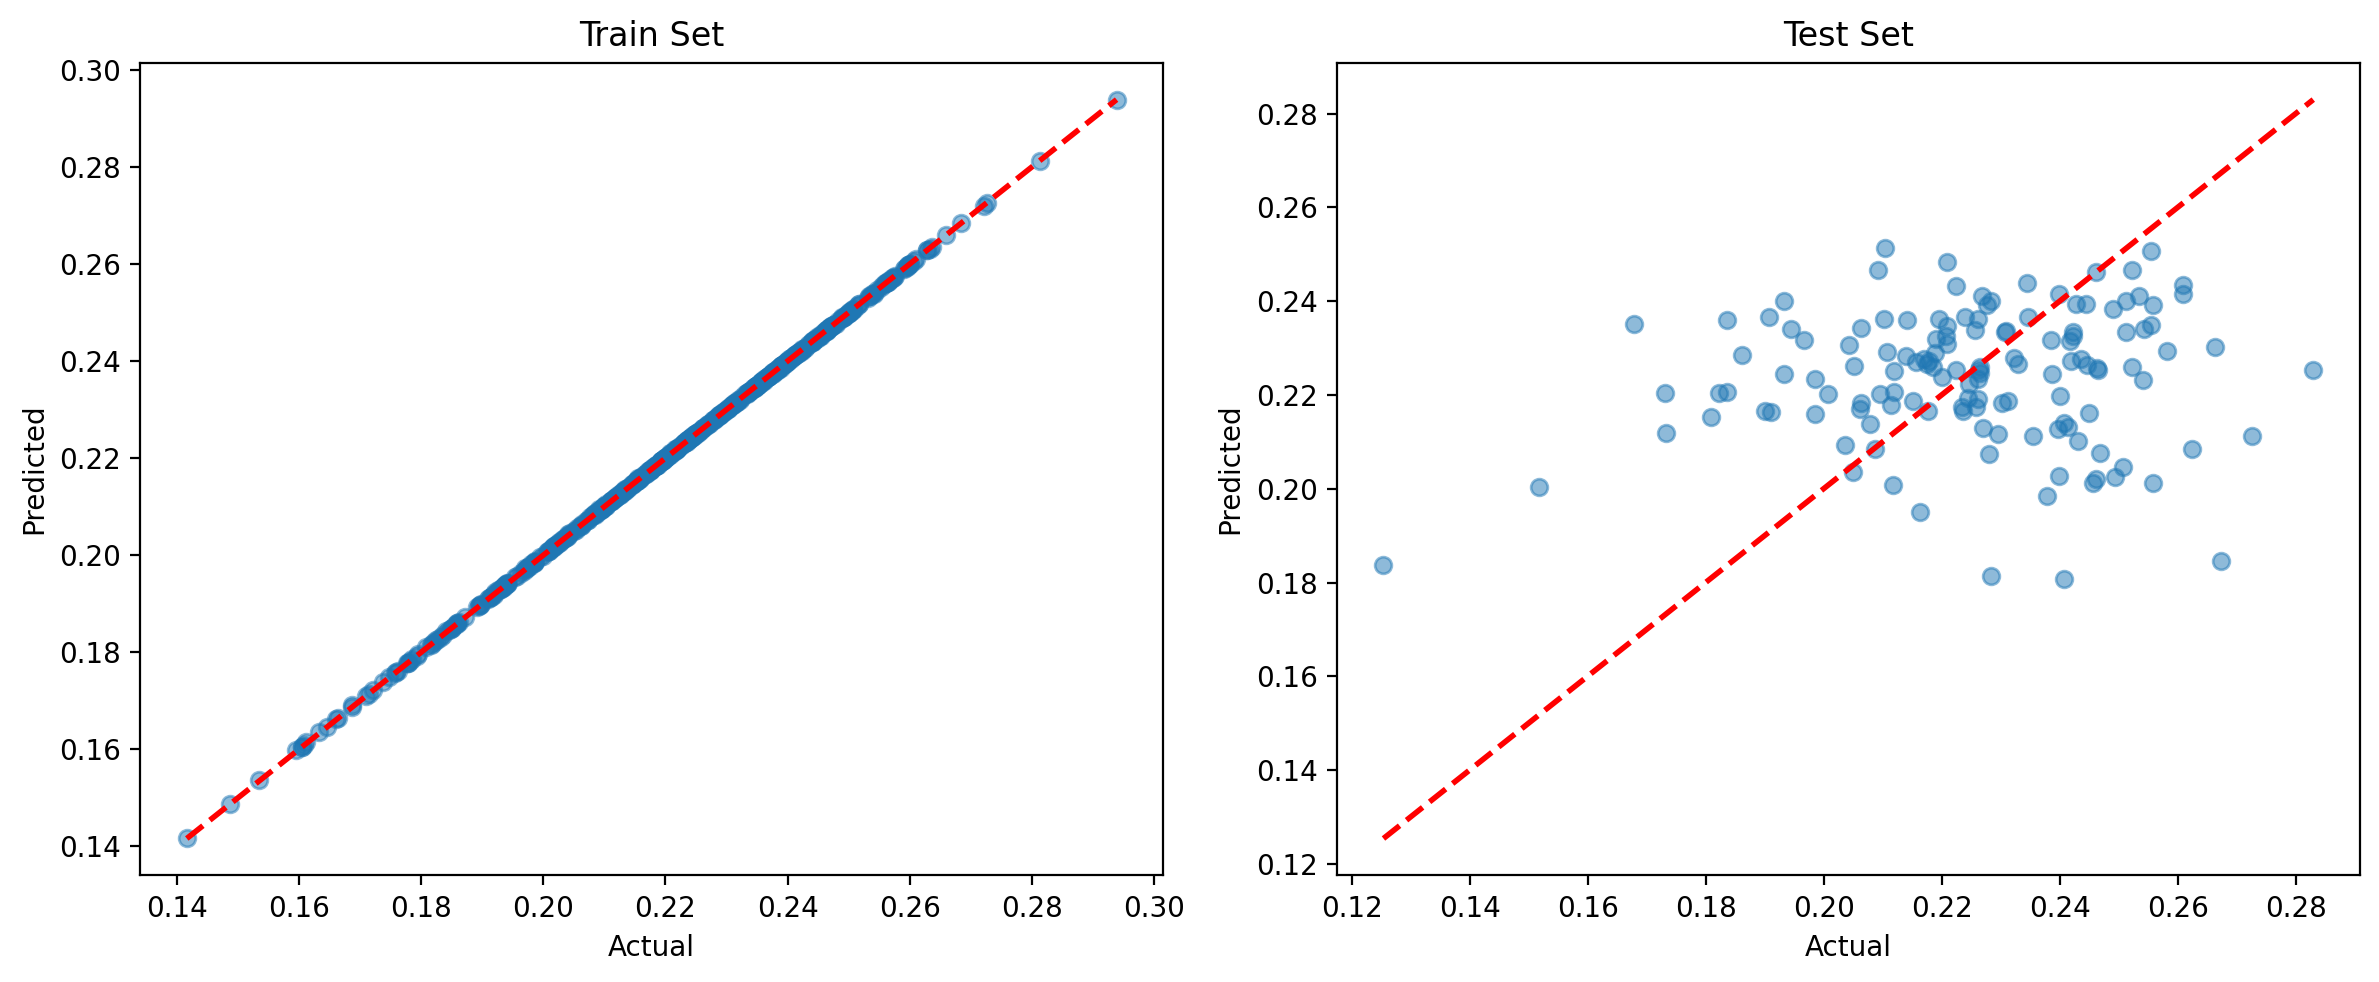
\includegraphics[width=12.38542in,height=5.11458in]{xgboost_tuned_files/figure-pdf/cell-41-output-2.png}

\includegraphics[width=49.80208in,height=41.09375in]{xgboost_tuned_files/figure-pdf/cell-41-output-3.png}

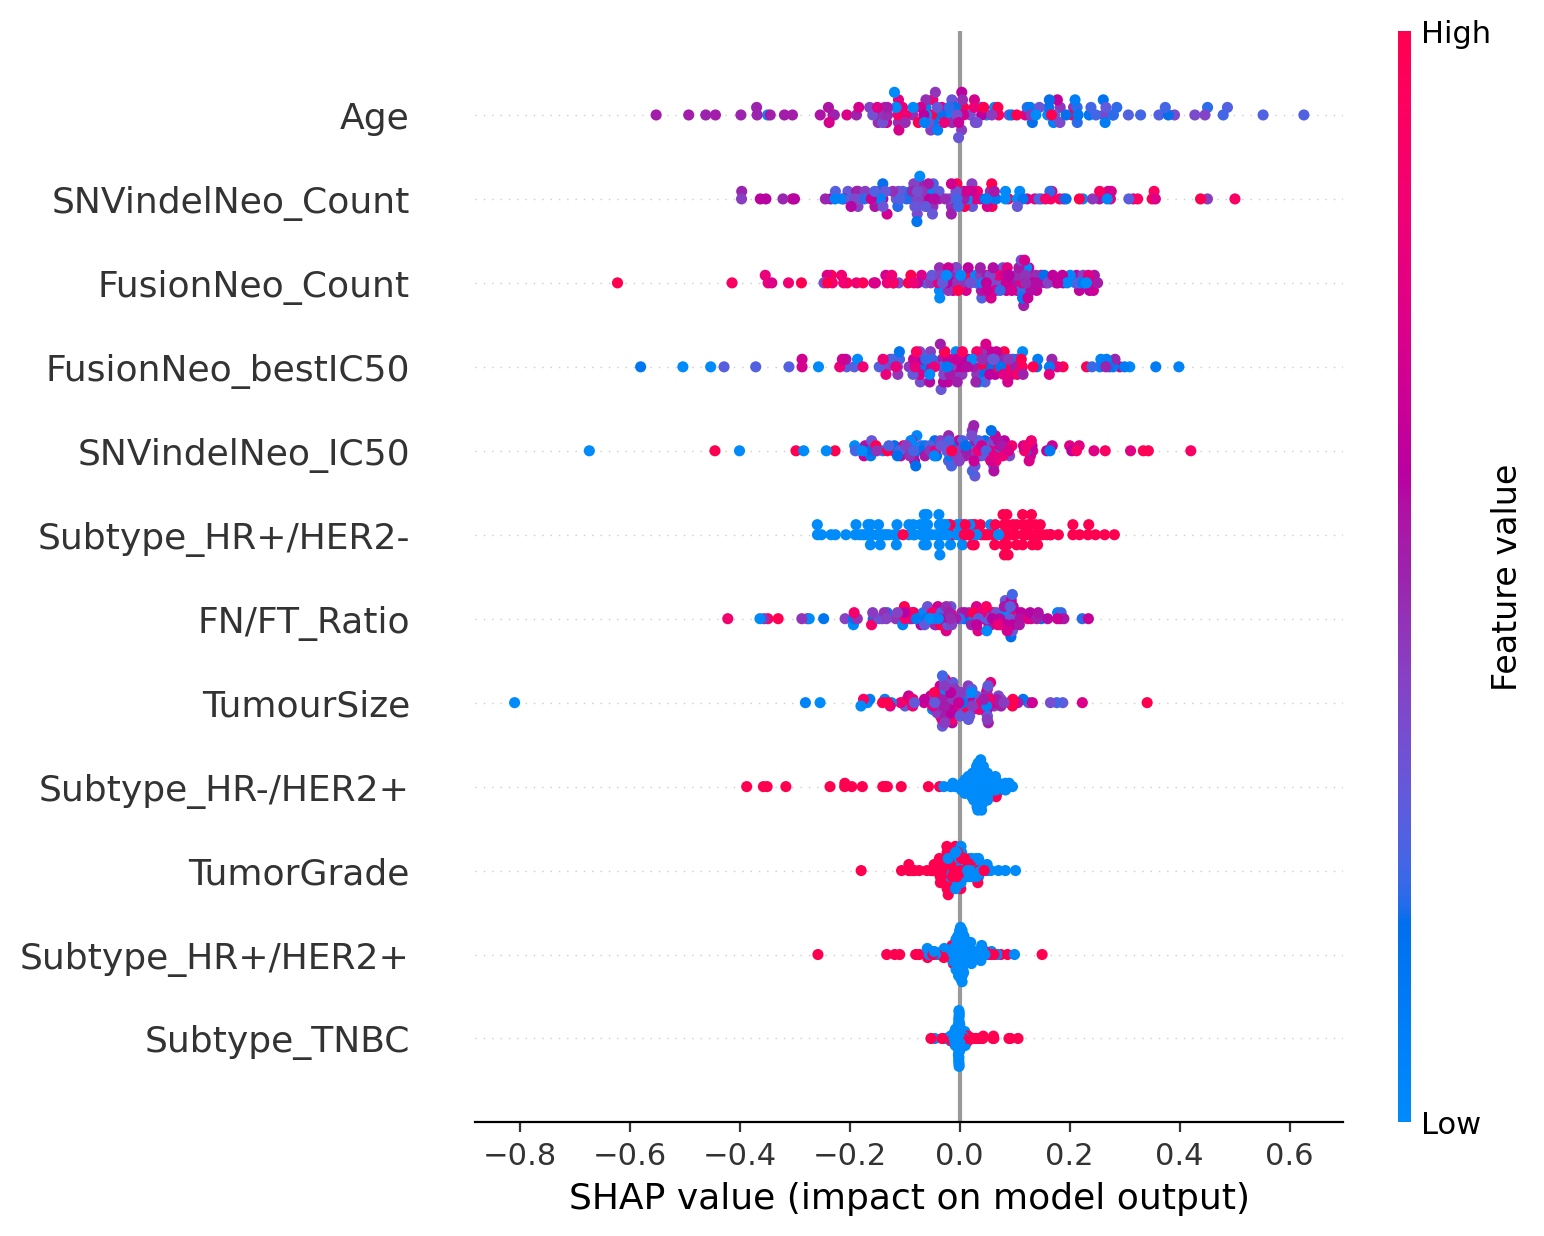
\includegraphics[width=8.04167in,height=6.4375in]{xgboost_tuned_files/figure-pdf/cell-41-output-4.png}

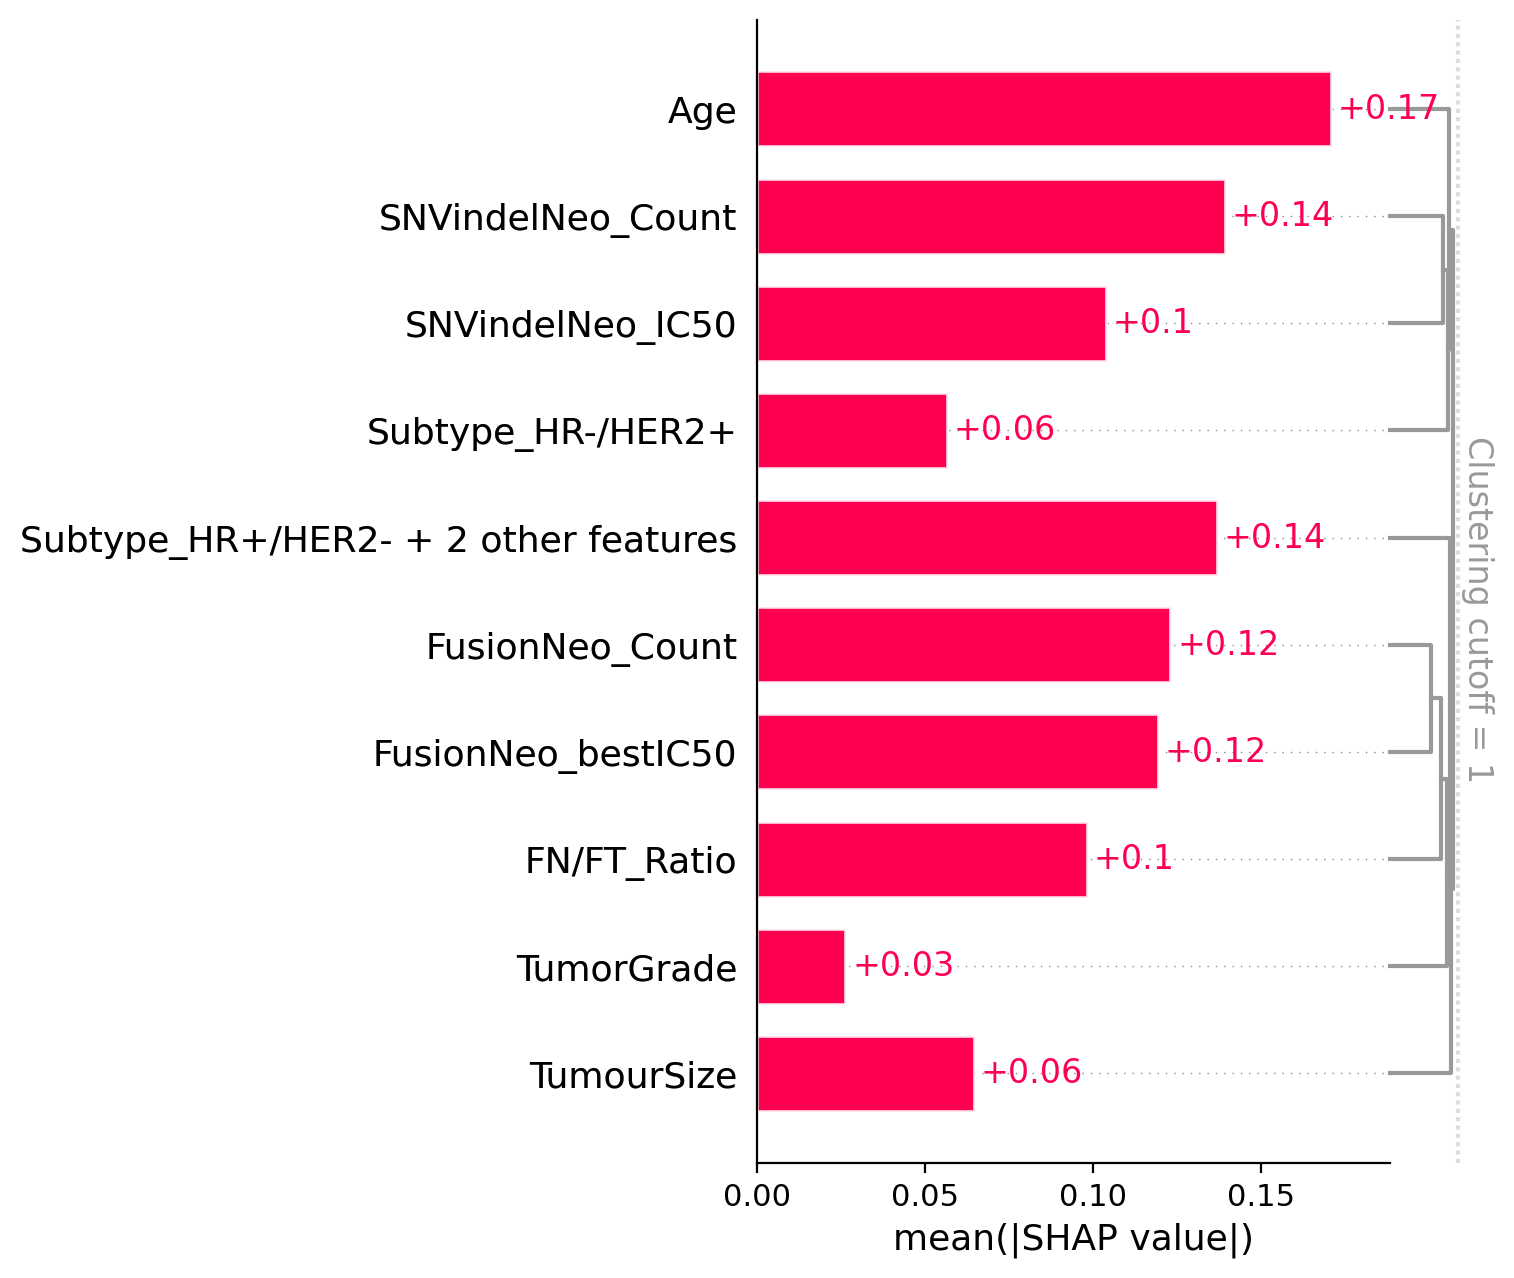
\includegraphics[width=7.88542in,height=6.65625in]{xgboost_tuned_files/figure-pdf/cell-41-output-5.png}

\paragraph{\texorpdfstring{\textbf{Iterative Learning over all Y
labels}}{Iterative Learning over all Y labels}}\label{iterative-learning-over-all-y-labels}

The learning using XGBoost above was done on just one Y label, which is
the \texttt{ESTIMATE} column. Let's put these into a set of functions so
we can run this process iteratively on all Y columns we have set up.

\begin{Shaded}
\begin{Highlighting}[]
\CommentTok{\# copy the steps above as a function}
\ImportTok{import}\NormalTok{ os }
\ImportTok{import}\NormalTok{ shap}
\ImportTok{from}\NormalTok{ xgboost }\ImportTok{import}\NormalTok{ XGBRegressor}
\ImportTok{from}\NormalTok{ sklearn.model\_selection }\ImportTok{import}\NormalTok{ learning\_curve}
\ImportTok{from}\NormalTok{ sklearn.metrics }\ImportTok{import}\NormalTok{ mean\_absolute\_error, mean\_squared\_error, r2\_score}

\KeywordTok{class}\NormalTok{ YTargetMetrics:}
    \KeywordTok{def} \FunctionTok{\_\_init\_\_}\NormalTok{(}\VariableTok{self}\NormalTok{, target\_name, train\_r2, test\_r2, train\_rmse, test\_rmse, train\_mae, test\_mae):}
        \VariableTok{self}\NormalTok{.target\_name }\OperatorTok{=}\NormalTok{ target\_name}
        \VariableTok{self}\NormalTok{.train\_r2 }\OperatorTok{=}\NormalTok{ train\_r2}
        \VariableTok{self}\NormalTok{.test\_r2 }\OperatorTok{=}\NormalTok{ test\_r2}
        \VariableTok{self}\NormalTok{.train\_rmse }\OperatorTok{=}\NormalTok{ train\_rmse}
        \VariableTok{self}\NormalTok{.test\_rmse }\OperatorTok{=}\NormalTok{ test\_rmse}
        \VariableTok{self}\NormalTok{.train\_mae }\OperatorTok{=}\NormalTok{ train\_mae}
        \VariableTok{self}\NormalTok{.test\_mae }\OperatorTok{=}\NormalTok{ test\_mae}

    \KeywordTok{def} \FunctionTok{\_\_str\_\_}\NormalTok{(}\VariableTok{self}\NormalTok{):}
        \ControlFlowTok{return} \SpecialStringTok{f"""Model Performance for }\SpecialCharTok{\{}\VariableTok{self}\SpecialCharTok{.}\NormalTok{target\_name}\SpecialCharTok{\}}\SpecialStringTok{:}
\SpecialCharTok{\{}\StringTok{\textquotesingle{}Metric\textquotesingle{}}\SpecialCharTok{:\textless{}10\}}\SpecialStringTok{ }\SpecialCharTok{\{}\StringTok{\textquotesingle{}Train\textquotesingle{}}\SpecialCharTok{:\textless{}10\}}\SpecialStringTok{ }\SpecialCharTok{\{}\StringTok{\textquotesingle{}Test\textquotesingle{}}\SpecialCharTok{:\textless{}10\}}
\SpecialCharTok{\{}\StringTok{\textquotesingle{}{-}\textquotesingle{}} \OperatorTok{*} \DecValTok{30}\SpecialCharTok{\}}
\SpecialCharTok{\{}\StringTok{\textquotesingle{}R2\textquotesingle{}}\SpecialCharTok{:\textless{}10\}}\SpecialStringTok{ }\SpecialCharTok{\{}\VariableTok{self}\SpecialCharTok{.}\NormalTok{train\_r2}\SpecialCharTok{:\textless{}10.4f\}}\SpecialStringTok{ }\SpecialCharTok{\{}\VariableTok{self}\SpecialCharTok{.}\NormalTok{test\_r2}\SpecialCharTok{:\textless{}10.4f\}}
\SpecialCharTok{\{}\StringTok{\textquotesingle{}RMSE\textquotesingle{}}\SpecialCharTok{:\textless{}10\}}\SpecialStringTok{ }\SpecialCharTok{\{}\VariableTok{self}\SpecialCharTok{.}\NormalTok{train\_rmse}\SpecialCharTok{:\textless{}10.4f\}}\SpecialStringTok{ }\SpecialCharTok{\{}\VariableTok{self}\SpecialCharTok{.}\NormalTok{test\_rmse}\SpecialCharTok{:\textless{}10.4f\}}
\SpecialCharTok{\{}\StringTok{\textquotesingle{}MAE\textquotesingle{}}\SpecialCharTok{:\textless{}10\}}\SpecialStringTok{ }\SpecialCharTok{\{}\VariableTok{self}\SpecialCharTok{.}\NormalTok{train\_mae}\SpecialCharTok{:\textless{}10.4f\}}\SpecialStringTok{ }\SpecialCharTok{\{}\VariableTok{self}\SpecialCharTok{.}\NormalTok{test\_mae}\SpecialCharTok{:\textless{}10.4f\}}\SpecialStringTok{"""}

    \KeywordTok{def}\NormalTok{ to\_dict(}\VariableTok{self}\NormalTok{):}
        \ControlFlowTok{return}\NormalTok{ \{}
            \StringTok{\textquotesingle{}target\_name\textquotesingle{}}\NormalTok{: }\VariableTok{self}\NormalTok{.target\_name,}
            \StringTok{\textquotesingle{}train\_r2\textquotesingle{}}\NormalTok{: }\VariableTok{self}\NormalTok{.train\_r2,}
            \StringTok{\textquotesingle{}test\_r2\textquotesingle{}}\NormalTok{: }\VariableTok{self}\NormalTok{.test\_r2,}
            \StringTok{\textquotesingle{}train\_rmse\textquotesingle{}}\NormalTok{: }\VariableTok{self}\NormalTok{.train\_rmse,}
            \StringTok{\textquotesingle{}test\_rmse\textquotesingle{}}\NormalTok{: }\VariableTok{self}\NormalTok{.test\_rmse,}
            \StringTok{\textquotesingle{}train\_mae\textquotesingle{}}\NormalTok{: }\VariableTok{self}\NormalTok{.train\_mae,}
            \StringTok{\textquotesingle{}test\_mae\textquotesingle{}}\NormalTok{: }\VariableTok{self}\NormalTok{.test\_mae}
\NormalTok{        \}}

\KeywordTok{def}\NormalTok{ plot\_learning\_curves(estimator, X, y, target, cv}\OperatorTok{=}\DecValTok{5}\NormalTok{, train\_sizes}\OperatorTok{=}\NormalTok{np.linspace(}\FloatTok{.1}\NormalTok{, }\FloatTok{1.0}\NormalTok{, }\DecValTok{5}\NormalTok{)):}
\NormalTok{    train\_sizes, train\_scores, test\_scores }\OperatorTok{=}\NormalTok{ learning\_curve(}
\NormalTok{        estimator, X, y, cv}\OperatorTok{=}\NormalTok{cv, n\_jobs}\OperatorTok{={-}}\DecValTok{1}\NormalTok{, train\_sizes}\OperatorTok{=}\NormalTok{train\_sizes,}
\NormalTok{        scoring}\OperatorTok{=}\StringTok{\textquotesingle{}neg\_mean\_squared\_error\textquotesingle{}}\NormalTok{)}
    
\NormalTok{    train\_scores\_mean }\OperatorTok{=} \OperatorTok{{-}}\NormalTok{train\_scores.mean(axis}\OperatorTok{=}\DecValTok{1}\NormalTok{)}
\NormalTok{    train\_scores\_std }\OperatorTok{=}\NormalTok{ train\_scores.std(axis}\OperatorTok{=}\DecValTok{1}\NormalTok{)}
\NormalTok{    test\_scores\_mean }\OperatorTok{=} \OperatorTok{{-}}\NormalTok{test\_scores.mean(axis}\OperatorTok{=}\DecValTok{1}\NormalTok{)}
\NormalTok{    test\_scores\_std }\OperatorTok{=}\NormalTok{ test\_scores.std(axis}\OperatorTok{=}\DecValTok{1}\NormalTok{)}

\NormalTok{    plt.figure(figsize}\OperatorTok{=}\NormalTok{(}\DecValTok{10}\NormalTok{, }\DecValTok{6}\NormalTok{), dpi}\OperatorTok{=}\DecValTok{300}\NormalTok{)}
\NormalTok{    plt.title(}\StringTok{"Learning Curves"}\NormalTok{)}
\NormalTok{    plt.xlabel(}\StringTok{"Training examples"}\NormalTok{)}
\NormalTok{    plt.ylabel(}\StringTok{"Mean Squared Error"}\NormalTok{)}
\NormalTok{    plt.fill\_between(train\_sizes, train\_scores\_mean }\OperatorTok{{-}}\NormalTok{ train\_scores\_std,}
\NormalTok{                     train\_scores\_mean }\OperatorTok{+}\NormalTok{ train\_scores\_std, alpha}\OperatorTok{=}\FloatTok{0.1}\NormalTok{, color}\OperatorTok{=}\StringTok{"r"}\NormalTok{)}
\NormalTok{    plt.fill\_between(train\_sizes, test\_scores\_mean }\OperatorTok{{-}}\NormalTok{ test\_scores\_std,}
\NormalTok{                     test\_scores\_mean }\OperatorTok{+}\NormalTok{ test\_scores\_std, alpha}\OperatorTok{=}\FloatTok{0.1}\NormalTok{, color}\OperatorTok{=}\StringTok{"g"}\NormalTok{)}
\NormalTok{    plt.plot(train\_sizes, train\_scores\_mean, }\StringTok{\textquotesingle{}o{-}\textquotesingle{}}\NormalTok{, color}\OperatorTok{=}\StringTok{"r"}\NormalTok{, label}\OperatorTok{=}\StringTok{"Training score"}\NormalTok{)}
\NormalTok{    plt.plot(train\_sizes, test\_scores\_mean, }\StringTok{\textquotesingle{}o{-}\textquotesingle{}}\NormalTok{, color}\OperatorTok{=}\StringTok{"g"}\NormalTok{, label}\OperatorTok{=}\StringTok{"Cross{-}validation score"}\NormalTok{)}
\NormalTok{    plt.legend(loc}\OperatorTok{=}\StringTok{"best"}\NormalTok{)}

    \CommentTok{\# Create \textquotesingle{}plots\textquotesingle{} directory if it doesn\textquotesingle{}t exist}
\NormalTok{    os.makedirs(}\SpecialStringTok{f\textquotesingle{}plots/}\SpecialCharTok{\{}\NormalTok{target}\SpecialCharTok{\}}\SpecialStringTok{\textquotesingle{}}\NormalTok{, exist\_ok}\OperatorTok{=}\VariableTok{True}\NormalTok{)}

    \CommentTok{\# Save the plot}
\NormalTok{    plt.savefig(}\SpecialStringTok{f\textquotesingle{}plots/}\SpecialCharTok{\{}\NormalTok{target}\SpecialCharTok{\}}\SpecialStringTok{/}\SpecialCharTok{\{}\NormalTok{target}\SpecialCharTok{\}}\SpecialStringTok{{-}xgb{-}def{-}model{-}learning{-}curve.png\textquotesingle{}}\NormalTok{)}
\NormalTok{    plt.close()}

\KeywordTok{def}\NormalTok{ run\_xgboost\_model(y\_target, Y\_train, Y\_test, X\_train\_transformed, X\_test\_transformed, Y\_train\_transformed, Y\_test\_transformed, preprocess\_pipeline\_Y):}
    \CommentTok{\# assign untransformed, raw target data}
\NormalTok{    raw\_y\_train }\OperatorTok{=}\NormalTok{ Y\_train[y\_target]}
\NormalTok{    raw\_y\_test }\OperatorTok{=}\NormalTok{ Y\_test[y\_target]}

\NormalTok{    model\_instance }\OperatorTok{=}\NormalTok{ XGBRegressor(n\_estimators}\OperatorTok{=}\DecValTok{150}\NormalTok{, random\_state}\OperatorTok{=}\DecValTok{42}\NormalTok{)}

    \CommentTok{\# fit}
\NormalTok{    model\_instance.fit(X\_train\_transformed, Y\_train\_transformed[y\_target])}
    
    \CommentTok{\# predict}
\NormalTok{    y\_train\_pred\_transformed }\OperatorTok{=}\NormalTok{ model\_instance.predict(X\_train\_transformed)}
\NormalTok{    y\_test\_pred\_transformed }\OperatorTok{=}\NormalTok{ model\_instance.predict(X\_test\_transformed)}

    \CommentTok{\# Create a DataFrame with the same columns as the original y used in fit}
\NormalTok{    dummy\_train\_y }\OperatorTok{=}\NormalTok{ pd.DataFrame(}\DecValTok{0}\NormalTok{, index}\OperatorTok{=}\NormalTok{X\_train\_transformed.index, columns}\OperatorTok{=}\NormalTok{Y\_train\_transformed.columns)}
\NormalTok{    dummy\_train\_y[y\_target] }\OperatorTok{=}\NormalTok{ y\_train\_pred\_transformed}

\NormalTok{    dummy\_test\_y }\OperatorTok{=}\NormalTok{ pd.DataFrame(}\DecValTok{0}\NormalTok{, index}\OperatorTok{=}\NormalTok{X\_test\_transformed.index, columns}\OperatorTok{=}\NormalTok{Y\_test\_transformed.columns)}
\NormalTok{    dummy\_test\_y[y\_target] }\OperatorTok{=}\NormalTok{ y\_test\_pred\_transformed}

    \CommentTok{\# apply inverse transform}
\NormalTok{    dummy\_train\_y\_inv }\OperatorTok{=}\NormalTok{ preprocess\_pipeline\_Y.inverse\_transform(dummy\_train\_y)}
\NormalTok{    dummy\_test\_y\_inv }\OperatorTok{=}\NormalTok{ preprocess\_pipeline\_Y.inverse\_transform(dummy\_test\_y)}

    \CommentTok{\# Extract the relevant target column}
\NormalTok{    y\_train\_pred }\OperatorTok{=}\NormalTok{ dummy\_train\_y\_inv[y\_target].to\_numpy()}
\NormalTok{    y\_test\_pred }\OperatorTok{=}\NormalTok{ dummy\_test\_y\_inv[y\_target].to\_numpy()}

    \CommentTok{\# Evaluate model}
    \CommentTok{\# Calculate metrics}
\NormalTok{    train\_r2 }\OperatorTok{=}\NormalTok{ r2\_score(raw\_y\_train, y\_train\_pred)}
\NormalTok{    test\_r2 }\OperatorTok{=}\NormalTok{ r2\_score(raw\_y\_test, y\_test\_pred)}

\NormalTok{    train\_rmse }\OperatorTok{=}\NormalTok{ np.sqrt(mean\_squared\_error(raw\_y\_train, y\_train\_pred))}
\NormalTok{    test\_rmse }\OperatorTok{=}\NormalTok{ np.sqrt(mean\_squared\_error(raw\_y\_test, y\_test\_pred))}

\NormalTok{    train\_mae }\OperatorTok{=}\NormalTok{ mean\_absolute\_error(raw\_y\_train, y\_train\_pred)}
\NormalTok{    test\_mae }\OperatorTok{=}\NormalTok{ mean\_absolute\_error(raw\_y\_test, y\_test\_pred)}

    \CommentTok{\# Plot learning curves}
\NormalTok{    plot\_learning\_curves(model\_instance, X\_train\_transformed, Y\_train\_transformed[y\_target], y\_target)}

    \CommentTok{\# Print results}
    \CommentTok{\# print("Model Performance:")}
    \CommentTok{\# print(f"\{\textquotesingle{}Metric\textquotesingle{}:\textless{}10\} \{\textquotesingle{}Train\textquotesingle{}:\textless{}10\} \{\textquotesingle{}Test\textquotesingle{}:\textless{}10\}")}
    \CommentTok{\# print("{-}" * 30)}
    \CommentTok{\# print(f"\{\textquotesingle{}R2\textquotesingle{}:\textless{}10\} \{train\_r2:\textless{}10.4f\} \{test\_r2:\textless{}10.4f\}")}
    \CommentTok{\# print(f"\{\textquotesingle{}RMSE\textquotesingle{}:\textless{}10\} \{train\_rmse:\textless{}10.4f\} \{test\_rmse:\textless{}10.4f\}")}
    \CommentTok{\# print(f"\{\textquotesingle{}MAE\textquotesingle{}:\textless{}10\} \{train\_mae:\textless{}10.4f\} \{test\_mae:\textless{}10.4f\}")}

    \CommentTok{\# Plot actual vs predicted}
\NormalTok{    \_, (ax1, ax2) }\OperatorTok{=}\NormalTok{ plt.subplots(}\DecValTok{1}\NormalTok{, }\DecValTok{2}\NormalTok{, figsize}\OperatorTok{=}\NormalTok{(}\DecValTok{12}\NormalTok{, }\DecValTok{6}\NormalTok{), dpi}\OperatorTok{=}\DecValTok{300}\NormalTok{)}

\NormalTok{    ax1.scatter(raw\_y\_train, y\_train\_pred, alpha}\OperatorTok{=}\FloatTok{0.5}\NormalTok{)}
\NormalTok{    ax1.plot([raw\_y\_train.}\BuiltInTok{min}\NormalTok{(), raw\_y\_train.}\BuiltInTok{max}\NormalTok{()], [raw\_y\_train.}\BuiltInTok{min}\NormalTok{(), raw\_y\_train.}\BuiltInTok{max}\NormalTok{()], }\StringTok{\textquotesingle{}r{-}{-}\textquotesingle{}}\NormalTok{, lw}\OperatorTok{=}\DecValTok{2}\NormalTok{)}
\NormalTok{    ax1.set\_xlabel(}\StringTok{\textquotesingle{}Actual\textquotesingle{}}\NormalTok{)}
\NormalTok{    ax1.set\_ylabel(}\StringTok{\textquotesingle{}Predicted\textquotesingle{}}\NormalTok{)}
\NormalTok{    ax1.set\_title(}\StringTok{\textquotesingle{}Training Set\textquotesingle{}}\NormalTok{)}

\NormalTok{    ax2.scatter(raw\_y\_test, y\_test\_pred, alpha}\OperatorTok{=}\FloatTok{0.5}\NormalTok{)}
\NormalTok{    ax2.plot([raw\_y\_test.}\BuiltInTok{min}\NormalTok{(), raw\_y\_test.}\BuiltInTok{max}\NormalTok{()], [raw\_y\_test.}\BuiltInTok{min}\NormalTok{(), raw\_y\_test.}\BuiltInTok{max}\NormalTok{()], }\StringTok{\textquotesingle{}r{-}{-}\textquotesingle{}}\NormalTok{, lw}\OperatorTok{=}\DecValTok{2}\NormalTok{)}
\NormalTok{    ax2.set\_xlabel(}\StringTok{\textquotesingle{}Actual\textquotesingle{}}\NormalTok{)}
\NormalTok{    ax2.set\_ylabel(}\StringTok{\textquotesingle{}Predicted\textquotesingle{}}\NormalTok{)}
\NormalTok{    ax2.set\_title(}\StringTok{\textquotesingle{}Testing Set\textquotesingle{}}\NormalTok{)}

\NormalTok{    plt.tight\_layout()}

    \CommentTok{\# Create \textquotesingle{}plots\textquotesingle{} directory if it doesn\textquotesingle{}t exist}
\NormalTok{    os.makedirs(}\SpecialStringTok{f\textquotesingle{}plots/}\SpecialCharTok{\{}\NormalTok{y\_target}\SpecialCharTok{\}}\SpecialStringTok{\textquotesingle{}}\NormalTok{, exist\_ok}\OperatorTok{=}\VariableTok{True}\NormalTok{)}

\NormalTok{    plt.savefig(}\SpecialStringTok{f\textquotesingle{}plots/}\SpecialCharTok{\{}\NormalTok{y\_target}\SpecialCharTok{\}}\SpecialStringTok{/}\SpecialCharTok{\{}\NormalTok{y\_target}\SpecialCharTok{\}}\SpecialStringTok{{-}xgb{-}def{-}model{-}performance{-}comparison.png\textquotesingle{}}\NormalTok{)}
\NormalTok{    plt.close()}

    \CommentTok{\# Feature importance}
\NormalTok{    \_, ax }\OperatorTok{=}\NormalTok{ plt.subplots(figsize}\OperatorTok{=}\NormalTok{(}\DecValTok{18}\NormalTok{, }\DecValTok{16}\NormalTok{), dpi}\OperatorTok{=}\DecValTok{300}\NormalTok{)}
\NormalTok{    plot\_importance(model\_instance, ax}\OperatorTok{=}\NormalTok{ax)}

\NormalTok{    plt.savefig(}\SpecialStringTok{f"plots/}\SpecialCharTok{\{}\NormalTok{y\_target}\SpecialCharTok{\}}\SpecialStringTok{/}\SpecialCharTok{\{}\NormalTok{y\_target}\SpecialCharTok{\}}\SpecialStringTok{{-}xgb{-}def{-}model{-}test{-}set{-}feature{-}importance.png"}\NormalTok{)}
\NormalTok{    plt.close()}

    \CommentTok{\# Create the SHAP explainer}
\NormalTok{    explainer }\OperatorTok{=}\NormalTok{ shap.TreeExplainer(model\_instance)}

    \CommentTok{\# run explanation object on X\_test dataset because we don\textquotesingle{}t want to learn what the model learned from the X\_train data, but to see features that would influence predictions on new data}
\NormalTok{    shap\_values }\OperatorTok{=}\NormalTok{ explainer(X\_test\_transformed)}

\NormalTok{    plt.figure(figsize}\OperatorTok{=}\NormalTok{(}\DecValTok{18}\NormalTok{, }\DecValTok{16}\NormalTok{), dpi}\OperatorTok{=}\DecValTok{300}\NormalTok{) }
    \CommentTok{\# Summary plot}
\NormalTok{    shap.summary\_plot(shap\_values, show}\OperatorTok{=}\VariableTok{False}\NormalTok{)}
\NormalTok{    plt.tight\_layout()}
\NormalTok{    plt.savefig(}\SpecialStringTok{f"plots/}\SpecialCharTok{\{}\NormalTok{y\_target}\SpecialCharTok{\}}\SpecialStringTok{/}\SpecialCharTok{\{}\NormalTok{y\_target}\SpecialCharTok{\}}\SpecialStringTok{{-}xgb{-}def{-}model{-}test{-}set{-}SHAP{-}beeswarm.png"}\NormalTok{, bbox\_inches}\OperatorTok{=}\StringTok{\textquotesingle{}tight\textquotesingle{}}\NormalTok{)}
\NormalTok{    plt.close()}

    \CommentTok{\# Perform clustering}
\NormalTok{    clust }\OperatorTok{=}\NormalTok{ shap.utils.hclust(X\_test\_transformed, Y\_test\_transformed[y\_target])}
    \CommentTok{\# Create the bar plot with clustering}
\NormalTok{    plt.figure(figsize}\OperatorTok{=}\NormalTok{(}\DecValTok{18}\NormalTok{, }\DecValTok{16}\NormalTok{)) }
\NormalTok{    shap.plots.bar(shap\_values, clustering}\OperatorTok{=}\NormalTok{clust, clustering\_cutoff}\OperatorTok{=}\DecValTok{1}\NormalTok{, show}\OperatorTok{=}\VariableTok{False}\NormalTok{)}
\NormalTok{    plt.tight\_layout()}
\NormalTok{    plt.savefig(}\SpecialStringTok{f"plots/}\SpecialCharTok{\{}\NormalTok{y\_target}\SpecialCharTok{\}}\SpecialStringTok{/}\SpecialCharTok{\{}\NormalTok{y\_target}\SpecialCharTok{\}}\SpecialStringTok{{-}xgb{-}def{-}model{-}test{-}set{-}SHAP{-}summary.png"}\NormalTok{, dpi}\OperatorTok{=}\DecValTok{300}\NormalTok{, bbox\_inches}\OperatorTok{=}\StringTok{\textquotesingle{}tight\textquotesingle{}}\NormalTok{)}
\NormalTok{    plt.close()}

    \BuiltInTok{print}\NormalTok{(}\SpecialStringTok{f"Model training and evaluation for }\SpecialCharTok{\{}\NormalTok{y\_target}\SpecialCharTok{\}}\SpecialStringTok{ completed."}\NormalTok{)}

    \CommentTok{\# Instead of returning a tuple, return a YTargetMetrics object}
    \ControlFlowTok{return}\NormalTok{ YTargetMetrics(y\_target, train\_r2, test\_r2, train\_rmse, test\_rmse, train\_mae, test\_mae)}
\end{Highlighting}
\end{Shaded}

\paragraph{\texorpdfstring{\textbf{Grid Search: Using
\texttt{GridSearchCV} for Hyperparameter
Tuning}}{Grid Search: Using GridSearchCV for Hyperparameter Tuning}}\label{grid-search-using-gridsearchcv-for-hyperparameter-tuning}

\begin{Shaded}
\begin{Highlighting}[]
\ImportTok{from}\NormalTok{ sklearn.model\_selection }\ImportTok{import}\NormalTok{ GridSearchCV}
\ImportTok{from}\NormalTok{ xgboost }\ImportTok{import}\NormalTok{ XGBRegressor}

\KeywordTok{class}\NormalTok{ YTargetMetrics:}
    \KeywordTok{def} \FunctionTok{\_\_init\_\_}\NormalTok{(}\VariableTok{self}\NormalTok{, target\_name, test\_mae, test\_rmse, test\_r2):}
        \VariableTok{self}\NormalTok{.target\_name }\OperatorTok{=}\NormalTok{ target\_name}
        \VariableTok{self}\NormalTok{.test\_mae }\OperatorTok{=}\NormalTok{ test\_mae}
        \VariableTok{self}\NormalTok{.test\_rmse }\OperatorTok{=}\NormalTok{ test\_rmse}
        \VariableTok{self}\NormalTok{.test\_r2 }\OperatorTok{=}\NormalTok{ test\_r2}

    \KeywordTok{def} \FunctionTok{\_\_str\_\_}\NormalTok{(}\VariableTok{self}\NormalTok{):}
        \ControlFlowTok{return} \SpecialStringTok{f"""Model Performance for }\SpecialCharTok{\{}\VariableTok{self}\SpecialCharTok{.}\NormalTok{target\_name}\SpecialCharTok{\}}\SpecialStringTok{:}
\SpecialCharTok{\{}\StringTok{\textquotesingle{}Metric\textquotesingle{}}\SpecialCharTok{:\textless{}10\}}\SpecialStringTok{ }\SpecialCharTok{\{}\StringTok{\textquotesingle{}Test\textquotesingle{}}\SpecialCharTok{:\textless{}10\}}
\SpecialCharTok{\{}\StringTok{\textquotesingle{}{-}\textquotesingle{}} \OperatorTok{*} \DecValTok{20}\SpecialCharTok{\}}
\SpecialCharTok{\{}\StringTok{\textquotesingle{}MAE\textquotesingle{}}\SpecialCharTok{:\textless{}10\}}\SpecialStringTok{ }\SpecialCharTok{\{}\VariableTok{self}\SpecialCharTok{.}\NormalTok{test\_mae}\SpecialCharTok{:\textless{}10.4f\}}
\SpecialCharTok{\{}\StringTok{\textquotesingle{}RMSE\textquotesingle{}}\SpecialCharTok{:\textless{}10\}}\SpecialStringTok{ }\SpecialCharTok{\{}\VariableTok{self}\SpecialCharTok{.}\NormalTok{test\_rmse}\SpecialCharTok{:\textless{}10.4f\}}
\SpecialCharTok{\{}\StringTok{\textquotesingle{}R2\textquotesingle{}}\SpecialCharTok{:\textless{}10\}}\SpecialStringTok{ }\SpecialCharTok{\{}\VariableTok{self}\SpecialCharTok{.}\NormalTok{test\_r2}\SpecialCharTok{:\textless{}10.4f\}}\SpecialStringTok{"""}

    \KeywordTok{def}\NormalTok{ to\_dict(}\VariableTok{self}\NormalTok{):}
        \ControlFlowTok{return}\NormalTok{ \{}
            \StringTok{\textquotesingle{}target\_name\textquotesingle{}}\NormalTok{: }\VariableTok{self}\NormalTok{.target\_name,}
            \StringTok{\textquotesingle{}test\_mae\textquotesingle{}}\NormalTok{: }\VariableTok{self}\NormalTok{.test\_mae,}
            \StringTok{\textquotesingle{}test\_rmse\textquotesingle{}}\NormalTok{: }\VariableTok{self}\NormalTok{.test\_rmse,}
            \StringTok{\textquotesingle{}test\_r2\textquotesingle{}}\NormalTok{: }\VariableTok{self}\NormalTok{.test\_r2}
\NormalTok{        \}}


\KeywordTok{def}\NormalTok{ run\_grid\_search\_cv(model\_instance, target, search\_space, X\_train\_transformed, Y\_train\_transformed, output\_path):}
    \CommentTok{\# assign y target column}
\NormalTok{    y\_train\_target }\OperatorTok{=}\NormalTok{ Y\_train\_transformed[target]}
    
    \CommentTok{\# Set up grid search}
\NormalTok{    grid\_search }\OperatorTok{=}\NormalTok{ GridSearchCV(}
\NormalTok{    estimator}\OperatorTok{=}\NormalTok{model\_instance,}
\NormalTok{    param\_grid}\OperatorTok{=}\NormalTok{search\_space,}
\NormalTok{    cv}\OperatorTok{=}\DecValTok{5}\NormalTok{,}
\NormalTok{    refit}\OperatorTok{=}\StringTok{\textquotesingle{}r2\textquotesingle{}}\NormalTok{,}
\NormalTok{    scoring}\OperatorTok{=}\NormalTok{[}\StringTok{\textquotesingle{}r2\textquotesingle{}}\NormalTok{, }\StringTok{\textquotesingle{}neg\_root\_mean\_squared\_error\textquotesingle{}}\NormalTok{],}
\NormalTok{    n\_jobs}\OperatorTok{={-}}\DecValTok{1}\NormalTok{,  }\CommentTok{\# Use all available cores}
\NormalTok{    verbose}\OperatorTok{=}\DecValTok{1}
\NormalTok{    )}
    
    \BuiltInTok{print}\NormalTok{(}\SpecialStringTok{f"Running grid search on }\SpecialCharTok{\{}\NormalTok{target}\SpecialCharTok{\}}\SpecialStringTok{ column..."}\NormalTok{)}
    \CommentTok{\# Fit grid search}
\NormalTok{    grid\_search.fit(X\_train\_transformed, y\_train\_target)}

    \CommentTok{\# Get best parameters and model}
\NormalTok{    best\_params }\OperatorTok{=}\NormalTok{ grid\_search.best\_params\_}
\NormalTok{    best\_model }\OperatorTok{=}\NormalTok{ grid\_search.best\_estimator\_}
\NormalTok{    best\_metric }\OperatorTok{=}\NormalTok{ grid\_search.best\_score\_}

    \BuiltInTok{print}\NormalTok{(}\StringTok{"Best parameters:"}\NormalTok{, best\_params)}
    \BuiltInTok{print}\NormalTok{(}\StringTok{"Best score:"}\NormalTok{, best\_metric)}

    \CommentTok{\# get CV results into a csv file}
\NormalTok{    cv\_results }\OperatorTok{=}\NormalTok{ pd.DataFrame(grid\_search.cv\_results\_)}
\NormalTok{    cv\_results }\OperatorTok{=}\NormalTok{ cv\_results.sort\_values(by}\OperatorTok{=}\StringTok{\textquotesingle{}rank\_test\_r2\textquotesingle{}}\NormalTok{)}
\NormalTok{    cv\_results.to\_csv(}\SpecialStringTok{f\textquotesingle{}}\SpecialCharTok{\{}\NormalTok{output\_path}\SpecialCharTok{\}}\SpecialStringTok{/grid\_search\_results\_}\SpecialCharTok{\{}\NormalTok{target}\SpecialCharTok{\}}\SpecialStringTok{\_score{-}}\SpecialCharTok{\{}\NormalTok{best\_metric}\SpecialCharTok{\}}\SpecialStringTok{.csv\textquotesingle{}}\NormalTok{, index}\OperatorTok{=}\VariableTok{False}\NormalTok{)}
    \ControlFlowTok{return}\NormalTok{ best\_model, best\_params, best\_metric}

\KeywordTok{def}\NormalTok{ predict\_with\_best\_xgboost\_model(best\_model, target, X\_test\_transformed, Y\_test\_transformed, Y\_test, preprocess\_pipeline\_Y):}
    \CommentTok{\# Make predictions on the test set using the best model}
\NormalTok{    y\_pred\_transformed }\OperatorTok{=}\NormalTok{ best\_model.predict(X\_test\_transformed)}

    \CommentTok{\# Create a DataFrame with the same columns as the original y used in preprocess\_pipeline to reverse transformation}
\NormalTok{    dummy\_df }\OperatorTok{=}\NormalTok{ pd.DataFrame(}\DecValTok{0}\NormalTok{, index}\OperatorTok{=}\NormalTok{X\_test\_transformed.index, columns}\OperatorTok{=}\NormalTok{Y\_test\_transformed.columns)}
\NormalTok{    dummy\_df[target] }\OperatorTok{=}\NormalTok{ y\_pred\_transformed}

    \CommentTok{\# apply inverse transform}
\NormalTok{    dummy\_df\_inv }\OperatorTok{=}\NormalTok{ preprocess\_pipeline\_Y.inverse\_transform(dummy\_df)}

    \CommentTok{\# Extract the relevant target column}
\NormalTok{    y\_pred }\OperatorTok{=}\NormalTok{ dummy\_df\_inv[target].to\_numpy()}

    \CommentTok{\# Evaluate}
\NormalTok{    y\_test }\OperatorTok{=}\NormalTok{ Y\_test[target]}
\NormalTok{    test\_mae }\OperatorTok{=}\NormalTok{ mean\_absolute\_error(y\_test, y\_pred)}
\NormalTok{    test\_rmse }\OperatorTok{=}\NormalTok{ np.sqrt(mean\_squared\_error(y\_test, y\_pred))}
\NormalTok{    test\_r2 }\OperatorTok{=}\NormalTok{ r2\_score(y\_test, y\_pred)}

    \BuiltInTok{print}\NormalTok{(}\SpecialStringTok{f"Mean Absolute Error (MAE) [Testing]: }\SpecialCharTok{\{}\NormalTok{test\_mae}\SpecialCharTok{:.2f\}}\SpecialStringTok{"}\NormalTok{)}
    \BuiltInTok{print}\NormalTok{(}\SpecialStringTok{f"Root Mean Squared Error (RMSE) [Testing]: }\SpecialCharTok{\{}\NormalTok{test\_rmse}\SpecialCharTok{:.2f\}}\SpecialStringTok{"}\NormalTok{)}
    \BuiltInTok{print}\NormalTok{(}\SpecialStringTok{f"Coefficient of Determination (R2) [Testing]: }\SpecialCharTok{\{}\NormalTok{test\_r2}\SpecialCharTok{:.2f\}}\SpecialStringTok{"}\NormalTok{)}

    \CommentTok{\# Instead of returning a tuple, return a YTargetMetrics object}
    \ControlFlowTok{return}\NormalTok{ YTargetMetrics(target, test\_mae, test\_rmse, test\_r2)}
\end{Highlighting}
\end{Shaded}

\begin{Shaded}
\begin{Highlighting}[]
\CommentTok{\# Instantiate base model}
\NormalTok{model\_xgb }\OperatorTok{=}\NormalTok{ XGBRegressor(random\_state}\OperatorTok{=}\DecValTok{42}\NormalTok{)}

\CommentTok{\# Define search space}
\NormalTok{search\_space }\OperatorTok{=}\NormalTok{ \{}
    \StringTok{\textquotesingle{}n\_estimators\textquotesingle{}}\NormalTok{: [}\DecValTok{100}\NormalTok{, }\DecValTok{200}\NormalTok{, }\DecValTok{400}\NormalTok{],}
    \StringTok{\textquotesingle{}max\_depth\textquotesingle{}}\NormalTok{: [}\DecValTok{3}\NormalTok{, }\DecValTok{6}\NormalTok{, }\DecValTok{9}\NormalTok{],}
    \StringTok{\textquotesingle{}learning\_rate\textquotesingle{}}\NormalTok{: [}\FloatTok{0.01}\NormalTok{, }\FloatTok{0.1}\NormalTok{, }\FloatTok{0.5}\NormalTok{, }\DecValTok{1}\NormalTok{],}
    \StringTok{\textquotesingle{}subsample\textquotesingle{}}\NormalTok{: [}\FloatTok{0.5}\NormalTok{, }\FloatTok{0.8}\NormalTok{, }\FloatTok{1.0}\NormalTok{],}
    \StringTok{\textquotesingle{}gamma\textquotesingle{}}\NormalTok{: [}\FloatTok{0.01}\NormalTok{, }\FloatTok{0.1}\NormalTok{]}
\NormalTok{\}}
\CommentTok{\# set output folder}
\NormalTok{output\_loc }\OperatorTok{=} \StringTok{\textquotesingle{}../nb/out\_files\textquotesingle{}}
\CommentTok{\# initialize an empty dict}
\NormalTok{tuned\_results }\OperatorTok{=}\NormalTok{ \{\}}

\ControlFlowTok{for}\NormalTok{ target }\KeywordTok{in}\NormalTok{ Y\_labels\_all:}
\NormalTok{    best\_model, best\_params, best\_metric }\OperatorTok{=}\NormalTok{ run\_grid\_search\_cv(model\_xgb, target, search\_space, X\_train\_yjs, Y\_train\_yjs, output\_loc)}
    
\NormalTok{    tuned\_metrics }\OperatorTok{=}\NormalTok{ predict\_with\_best\_xgboost\_model(best\_model, target, X\_test\_yjs, Y\_test\_yjs, Y\_test, preprocess\_pipeline\_Y)}

    \CommentTok{\# Store the metric result in the dictionary}
\NormalTok{    tuned\_results[target] }\OperatorTok{=}\NormalTok{ tuned\_metrics}
\end{Highlighting}
\end{Shaded}

\begin{verbatim}
Running grid search on ESTIMATE column...
Fitting 5 folds for each of 216 candidates, totalling 1080 fits
Best parameters: {'gamma': 0.01, 'learning_rate': 0.01, 'max_depth': 3, 'n_estimators': 400, 'subsample': 0.5}
Best score: 0.155118346758868
Mean Absolute Error (MAE) [Testing]: 952.47
Root Mean Squared Error (RMSE) [Testing]: 1176.54
Coefficient of Determination (R2) [Testing]: 0.17
Running grid search on IMPRES column...
Fitting 5 folds for each of 216 candidates, totalling 1080 fits
Best parameters: {'gamma': 0.01, 'learning_rate': 0.01, 'max_depth': 6, 'n_estimators': 100, 'subsample': 0.5}
Best score: 0.02365982741447383
Mean Absolute Error (MAE) [Testing]: 1.05
Root Mean Squared Error (RMSE) [Testing]: 1.31
Coefficient of Determination (R2) [Testing]: 0.03
Running grid search on C_Bcellsnaive column...
Fitting 5 folds for each of 216 candidates, totalling 1080 fits
Best parameters: {'gamma': 0.01, 'learning_rate': 0.01, 'max_depth': 3, 'n_estimators': 200, 'subsample': 0.5}
Best score: 0.05135495163777317
Mean Absolute Error (MAE) [Testing]: 0.04
Root Mean Squared Error (RMSE) [Testing]: 0.05
Coefficient of Determination (R2) [Testing]: 0.08
Running grid search on C_TcellsCD4memoryresting column...
Fitting 5 folds for each of 216 candidates, totalling 1080 fits
Best parameters: {'gamma': 0.01, 'learning_rate': 0.01, 'max_depth': 3, 'n_estimators': 100, 'subsample': 0.5}
Best score: -0.028307017274827716
Mean Absolute Error (MAE) [Testing]: 0.07
Root Mean Squared Error (RMSE) [Testing]: 0.08
Coefficient of Determination (R2) [Testing]: 0.00
Running grid search on C_MacrophagesM2 column...
Fitting 5 folds for each of 216 candidates, totalling 1080 fits
Best parameters: {'gamma': 0.1, 'learning_rate': 0.01, 'max_depth': 9, 'n_estimators': 100, 'subsample': 0.5}
Best score: 0.029962885460540156
Mean Absolute Error (MAE) [Testing]: 0.08
Root Mean Squared Error (RMSE) [Testing]: 0.10
Coefficient of Determination (R2) [Testing]: 0.02
Running grid search on S_Attractors_LYM column...
Fitting 5 folds for each of 216 candidates, totalling 1080 fits
Best parameters: {'gamma': 0.1, 'learning_rate': 0.01, 'max_depth': 3, 'n_estimators': 400, 'subsample': 0.8}
Best score: 0.1519325801004562
Mean Absolute Error (MAE) [Testing]: 0.03
Root Mean Squared Error (RMSE) [Testing]: 0.04
Coefficient of Determination (R2) [Testing]: 0.12
Running grid search on S_Attractors_IFIT3 column...
Fitting 5 folds for each of 216 candidates, totalling 1080 fits
Best parameters: {'gamma': 0.1, 'learning_rate': 0.01, 'max_depth': 3, 'n_estimators': 100, 'subsample': 0.5}
Best score: -0.01740592098092939
Mean Absolute Error (MAE) [Testing]: 0.04
Root Mean Squared Error (RMSE) [Testing]: 0.05
Coefficient of Determination (R2) [Testing]: 0.01
Running grid search on S_Attractors_G_GIMAP4 column...
Fitting 5 folds for each of 216 candidates, totalling 1080 fits
Best parameters: {'gamma': 0.01, 'learning_rate': 0.01, 'max_depth': 3, 'n_estimators': 200, 'subsample': 0.8}
Best score: 0.10172485511123637
Mean Absolute Error (MAE) [Testing]: 0.03
Root Mean Squared Error (RMSE) [Testing]: 0.04
Coefficient of Determination (R2) [Testing]: 0.11
Running grid search on S_Attractors_G_HLA.DPA1 column...
Fitting 5 folds for each of 216 candidates, totalling 1080 fits
Best parameters: {'gamma': 0.1, 'learning_rate': 0.01, 'max_depth': 3, 'n_estimators': 400, 'subsample': 1.0}
Best score: 0.13334587343594612
Mean Absolute Error (MAE) [Testing]: 0.02
Root Mean Squared Error (RMSE) [Testing]: 0.03
Coefficient of Determination (R2) [Testing]: -0.02
Running grid search on S_Attractors_G_SLAMF6 column...
Fitting 5 folds for each of 216 candidates, totalling 1080 fits
Best parameters: {'gamma': 0.1, 'learning_rate': 0.01, 'max_depth': 3, 'n_estimators': 400, 'subsample': 0.5}
Best score: 0.19095641111048084
Mean Absolute Error (MAE) [Testing]: 0.04
Root Mean Squared Error (RMSE) [Testing]: 0.05
Coefficient of Determination (R2) [Testing]: 0.17
Running grid search on S_Attractors_G_LILRB4 column...
Fitting 5 folds for each of 216 candidates, totalling 1080 fits
Best parameters: {'gamma': 0.1, 'learning_rate': 0.01, 'max_depth': 3, 'n_estimators': 400, 'subsample': 0.8}
Best score: 0.14469212473633178
Mean Absolute Error (MAE) [Testing]: 0.02
Root Mean Squared Error (RMSE) [Testing]: 0.03
Coefficient of Determination (R2) [Testing]: 0.09
Running grid search on S_Attractors_G_SIGLEC9 column...
Fitting 5 folds for each of 216 candidates, totalling 1080 fits
Best parameters: {'gamma': 0.01, 'learning_rate': 0.01, 'max_depth': 3, 'n_estimators': 100, 'subsample': 0.5}
Best score: -0.02085049620339232
Mean Absolute Error (MAE) [Testing]: 0.03
Root Mean Squared Error (RMSE) [Testing]: 0.04
Coefficient of Determination (R2) [Testing]: 0.00
Running grid search on S_Attractors_G_CYTH4 column...
Fitting 5 folds for each of 216 candidates, totalling 1080 fits
Best parameters: {'gamma': 0.01, 'learning_rate': 0.01, 'max_depth': 3, 'n_estimators': 400, 'subsample': 0.5}
Best score: 0.16852131461885284
Mean Absolute Error (MAE) [Testing]: 0.03
Root Mean Squared Error (RMSE) [Testing]: 0.04
Coefficient of Determination (R2) [Testing]: 0.18
Running grid search on S_Attractors_G_CD3E column...
Fitting 5 folds for each of 216 candidates, totalling 1080 fits
Best parameters: {'gamma': 0.01, 'learning_rate': 0.01, 'max_depth': 3, 'n_estimators': 400, 'subsample': 0.5}
Best score: 0.1360970322747118
Mean Absolute Error (MAE) [Testing]: 0.04
Root Mean Squared Error (RMSE) [Testing]: 0.05
Coefficient of Determination (R2) [Testing]: 0.13
Running grid search on S_Lymph_Vessels column...
Fitting 5 folds for each of 216 candidates, totalling 1080 fits
Best parameters: {'gamma': 0.01, 'learning_rate': 0.01, 'max_depth': 6, 'n_estimators': 100, 'subsample': 0.5}
Best score: 0.03201288157917721
Mean Absolute Error (MAE) [Testing]: 0.03
Root Mean Squared Error (RMSE) [Testing]: 0.03
Coefficient of Determination (R2) [Testing]: -0.02
Running grid search on S_ICR_SCORE column...
Fitting 5 folds for each of 216 candidates, totalling 1080 fits
Best parameters: {'gamma': 0.1, 'learning_rate': 0.01, 'max_depth': 3, 'n_estimators': 400, 'subsample': 0.8}
Best score: 0.15934291353526212
Mean Absolute Error (MAE) [Testing]: 0.04
Root Mean Squared Error (RMSE) [Testing]: 0.05
Coefficient of Determination (R2) [Testing]: 0.13
Running grid search on S_ICR_INHIB_SCORE column...
Fitting 5 folds for each of 216 candidates, totalling 1080 fits
Best parameters: {'gamma': 0.01, 'learning_rate': 0.01, 'max_depth': 3, 'n_estimators': 200, 'subsample': 0.5}
Best score: 0.1627773250826052
Mean Absolute Error (MAE) [Testing]: 0.03
Root Mean Squared Error (RMSE) [Testing]: 0.04
Coefficient of Determination (R2) [Testing]: 0.18
Running grid search on S_ICR_ACT_SCORE column...
Fitting 5 folds for each of 216 candidates, totalling 1080 fits
Best parameters: {'gamma': 0.1, 'learning_rate': 0.01, 'max_depth': 3, 'n_estimators': 400, 'subsample': 0.8}
Best score: 0.1530260099969623
Mean Absolute Error (MAE) [Testing]: 0.04
Root Mean Squared Error (RMSE) [Testing]: 0.05
Coefficient of Determination (R2) [Testing]: 0.12
Running grid search on S_Angiogenesis column...
Fitting 5 folds for each of 216 candidates, totalling 1080 fits
Best parameters: {'gamma': 0.1, 'learning_rate': 0.01, 'max_depth': 3, 'n_estimators': 200, 'subsample': 0.8}
Best score: 0.06861915844628179
Mean Absolute Error (MAE) [Testing]: 0.02
Root Mean Squared Error (RMSE) [Testing]: 0.03
Coefficient of Determination (R2) [Testing]: 0.03
Running grid search on S_APM1 column...
Fitting 5 folds for each of 216 candidates, totalling 1080 fits
Best parameters: {'gamma': 0.01, 'learning_rate': 0.01, 'max_depth': 3, 'n_estimators': 200, 'subsample': 0.5}
Best score: 0.09787115491563478
Mean Absolute Error (MAE) [Testing]: 0.01
Root Mean Squared Error (RMSE) [Testing]: 0.01
Coefficient of Determination (R2) [Testing]: 0.12
Running grid search on S_APM2 column...
Fitting 5 folds for each of 216 candidates, totalling 1080 fits
Best parameters: {'gamma': 0.01, 'learning_rate': 0.01, 'max_depth': 3, 'n_estimators': 200, 'subsample': 0.5}
Best score: 0.07828700996075295
Mean Absolute Error (MAE) [Testing]: 0.02
Root Mean Squared Error (RMSE) [Testing]: 0.03
Coefficient of Determination (R2) [Testing]: 0.06
Running grid search on S_ICS5_score column...
Fitting 5 folds for each of 216 candidates, totalling 1080 fits
Best parameters: {'gamma': 0.1, 'learning_rate': 0.01, 'max_depth': 3, 'n_estimators': 400, 'subsample': 0.5}
Best score: 0.1663422797208908
Mean Absolute Error (MAE) [Testing]: 0.04
Root Mean Squared Error (RMSE) [Testing]: 0.06
Coefficient of Determination (R2) [Testing]: 0.07
Running grid search on S_LIexpression_score column...
Fitting 5 folds for each of 216 candidates, totalling 1080 fits
Best parameters: {'gamma': 0.01, 'learning_rate': 0.01, 'max_depth': 3, 'n_estimators': 400, 'subsample': 0.5}
Best score: 0.19099609728572745
Mean Absolute Error (MAE) [Testing]: 0.04
Root Mean Squared Error (RMSE) [Testing]: 0.05
Coefficient of Determination (R2) [Testing]: 0.16
Running grid search on S_Chemokine12_score column...
Fitting 5 folds for each of 216 candidates, totalling 1080 fits
Best parameters: {'gamma': 0.01, 'learning_rate': 0.01, 'max_depth': 3, 'n_estimators': 200, 'subsample': 0.8}
Best score: 0.1804485480291262
Mean Absolute Error (MAE) [Testing]: 0.04
Root Mean Squared Error (RMSE) [Testing]: 0.05
Coefficient of Determination (R2) [Testing]: 0.13
Running grid search on S_NHI_5gene_score column...
Fitting 5 folds for each of 216 candidates, totalling 1080 fits
Best parameters: {'gamma': 0.01, 'learning_rate': 0.01, 'max_depth': 3, 'n_estimators': 400, 'subsample': 0.5}
Best score: 0.1345919647519557
Mean Absolute Error (MAE) [Testing]: 0.02
Root Mean Squared Error (RMSE) [Testing]: 0.03
Coefficient of Determination (R2) [Testing]: 0.08
Running grid search on S_CD68 column...
Fitting 5 folds for each of 216 candidates, totalling 1080 fits
Best parameters: {'gamma': 0.01, 'learning_rate': 0.01, 'max_depth': 9, 'n_estimators': 100, 'subsample': 0.5}
Best score: 0.03917842665714646
Mean Absolute Error (MAE) [Testing]: 0.08
Root Mean Squared Error (RMSE) [Testing]: 0.13
Coefficient of Determination (R2) [Testing]: -0.14
Running grid search on S_CD8A column...
Fitting 5 folds for each of 216 candidates, totalling 1080 fits
Best parameters: {'gamma': 0.01, 'learning_rate': 0.01, 'max_depth': 3, 'n_estimators': 400, 'subsample': 0.5}
Best score: 0.09649175911751913
Mean Absolute Error (MAE) [Testing]: 0.04
Root Mean Squared Error (RMSE) [Testing]: 0.06
Coefficient of Determination (R2) [Testing]: 0.11
Running grid search on S_PD1_data column...
Fitting 5 folds for each of 216 candidates, totalling 1080 fits
Best parameters: {'gamma': 0.01, 'learning_rate': 0.01, 'max_depth': 3, 'n_estimators': 400, 'subsample': 0.8}
Best score: 0.1388274399040847
Mean Absolute Error (MAE) [Testing]: 0.05
Root Mean Squared Error (RMSE) [Testing]: 0.09
Coefficient of Determination (R2) [Testing]: -0.01
Running grid search on S_PDL1_data column...
Fitting 5 folds for each of 216 candidates, totalling 1080 fits
Best parameters: {'gamma': 0.1, 'learning_rate': 0.01, 'max_depth': 3, 'n_estimators': 200, 'subsample': 0.8}
Best score: 0.09523166841467698
Mean Absolute Error (MAE) [Testing]: 0.03
Root Mean Squared Error (RMSE) [Testing]: 0.04
Coefficient of Determination (R2) [Testing]: 0.08
Running grid search on S_PD1_PDL1_score column...
Fitting 5 folds for each of 216 candidates, totalling 1080 fits
Best parameters: {'gamma': 0.01, 'learning_rate': 0.01, 'max_depth': 3, 'n_estimators': 400, 'subsample': 0.8}
Best score: 0.1223460942580558
Mean Absolute Error (MAE) [Testing]: 0.03
Root Mean Squared Error (RMSE) [Testing]: 0.05
Coefficient of Determination (R2) [Testing]: 0.04
Running grid search on S_CTLA4_data column...
Fitting 5 folds for each of 216 candidates, totalling 1080 fits
Best parameters: {'gamma': 0.01, 'learning_rate': 0.01, 'max_depth': 3, 'n_estimators': 200, 'subsample': 0.8}
Best score: 0.14432249434540673
Mean Absolute Error (MAE) [Testing]: 0.04
Root Mean Squared Error (RMSE) [Testing]: 0.06
Coefficient of Determination (R2) [Testing]: 0.07
Running grid search on S_Bcell_mg_IGJ column...
Fitting 5 folds for each of 216 candidates, totalling 1080 fits
Best parameters: {'gamma': 0.1, 'learning_rate': 0.01, 'max_depth': 3, 'n_estimators': 400, 'subsample': 0.5}
Best score: 0.15437226542586852
Mean Absolute Error (MAE) [Testing]: 0.05
Root Mean Squared Error (RMSE) [Testing]: 0.07
Coefficient of Determination (R2) [Testing]: -0.00
Running grid search on S_Bcell_receptors_score column...
Fitting 5 folds for each of 216 candidates, totalling 1080 fits
Best parameters: {'gamma': 0.1, 'learning_rate': 0.01, 'max_depth': 3, 'n_estimators': 400, 'subsample': 0.8}
Best score: 0.20872363643597835
Mean Absolute Error (MAE) [Testing]: 0.03
Root Mean Squared Error (RMSE) [Testing]: 0.03
Coefficient of Determination (R2) [Testing]: 0.17
Running grid search on S_STAT1_score column...
Fitting 5 folds for each of 216 candidates, totalling 1080 fits
Best parameters: {'gamma': 0.1, 'learning_rate': 0.01, 'max_depth': 3, 'n_estimators': 400, 'subsample': 0.5}
Best score: 0.10808145140828648
Mean Absolute Error (MAE) [Testing]: 0.02
Root Mean Squared Error (RMSE) [Testing]: 0.03
Coefficient of Determination (R2) [Testing]: 0.13
Running grid search on S_CSF1_response column...
Fitting 5 folds for each of 216 candidates, totalling 1080 fits
Best parameters: {'gamma': 0.01, 'learning_rate': 0.01, 'max_depth': 3, 'n_estimators': 400, 'subsample': 0.8}
Best score: 0.17036253048148878
Mean Absolute Error (MAE) [Testing]: 0.02
Root Mean Squared Error (RMSE) [Testing]: 0.03
Coefficient of Determination (R2) [Testing]: 0.12
Running grid search on S_TcClassII_score column...
Fitting 5 folds for each of 216 candidates, totalling 1080 fits
Best parameters: {'gamma': 0.1, 'learning_rate': 0.01, 'max_depth': 3, 'n_estimators': 400, 'subsample': 0.8}
Best score: 0.1353092427600878
Mean Absolute Error (MAE) [Testing]: 0.02
Root Mean Squared Error (RMSE) [Testing]: 0.03
Coefficient of Determination (R2) [Testing]: 0.13
Running grid search on S_IL12_score_21050467 column...
Fitting 5 folds for each of 216 candidates, totalling 1080 fits
Best parameters: {'gamma': 0.1, 'learning_rate': 0.01, 'max_depth': 3, 'n_estimators': 400, 'subsample': 0.5}
Best score: 0.1685925936656082
Mean Absolute Error (MAE) [Testing]: 0.02
Root Mean Squared Error (RMSE) [Testing]: 0.03
Coefficient of Determination (R2) [Testing]: 0.16
Running grid search on S_IL4_score_21050467 column...
Fitting 5 folds for each of 216 candidates, totalling 1080 fits
Best parameters: {'gamma': 0.1, 'learning_rate': 0.01, 'max_depth': 6, 'n_estimators': 200, 'subsample': 0.5}
Best score: 0.058610473096243496
Mean Absolute Error (MAE) [Testing]: 0.01
Root Mean Squared Error (RMSE) [Testing]: 0.02
Coefficient of Determination (R2) [Testing]: 0.04
Running grid search on S_IL2_score_21050467 column...
Fitting 5 folds for each of 216 candidates, totalling 1080 fits
Best parameters: {'gamma': 0.01, 'learning_rate': 0.01, 'max_depth': 3, 'n_estimators': 200, 'subsample': 0.5}
Best score: 0.10951936674694163
Mean Absolute Error (MAE) [Testing]: 0.01
Root Mean Squared Error (RMSE) [Testing]: 0.02
Coefficient of Determination (R2) [Testing]: 0.14
Running grid search on S_IL13_score_21050467 column...
Fitting 5 folds for each of 216 candidates, totalling 1080 fits
Best parameters: {'gamma': 0.01, 'learning_rate': 0.01, 'max_depth': 3, 'n_estimators': 100, 'subsample': 0.5}
Best score: -0.002331576883738795
Mean Absolute Error (MAE) [Testing]: 0.02
Root Mean Squared Error (RMSE) [Testing]: 0.03
Coefficient of Determination (R2) [Testing]: 0.03
Running grid search on S_IFNG_score_21050467 column...
Fitting 5 folds for each of 216 candidates, totalling 1080 fits
Best parameters: {'gamma': 0.01, 'learning_rate': 0.01, 'max_depth': 3, 'n_estimators': 400, 'subsample': 1.0}
Best score: 0.14472145870011874
Mean Absolute Error (MAE) [Testing]: 0.01
Root Mean Squared Error (RMSE) [Testing]: 0.01
Coefficient of Determination (R2) [Testing]: 0.13
Running grid search on S_TGFB_score_21050467 column...
Fitting 5 folds for each of 216 candidates, totalling 1080 fits
Best parameters: {'gamma': 0.01, 'learning_rate': 0.01, 'max_depth': 3, 'n_estimators': 200, 'subsample': 1.0}
Best score: 0.035040184707386325
Mean Absolute Error (MAE) [Testing]: 0.01
Root Mean Squared Error (RMSE) [Testing]: 0.01
Coefficient of Determination (R2) [Testing]: -0.03
Running grid search on S_TREM1_data column...
Fitting 5 folds for each of 216 candidates, totalling 1080 fits
Best parameters: {'gamma': 0.01, 'learning_rate': 0.01, 'max_depth': 3, 'n_estimators': 100, 'subsample': 1.0}
Best score: 0.05379798267792597
Mean Absolute Error (MAE) [Testing]: 0.04
Root Mean Squared Error (RMSE) [Testing]: 0.05
Coefficient of Determination (R2) [Testing]: 0.06
Running grid search on S_DAP12_data column...
Fitting 5 folds for each of 216 candidates, totalling 1080 fits
Best parameters: {'gamma': 0.1, 'learning_rate': 0.01, 'max_depth': 3, 'n_estimators': 400, 'subsample': 0.5}
Best score: 0.0826437020332194
Mean Absolute Error (MAE) [Testing]: 0.03
Root Mean Squared Error (RMSE) [Testing]: 0.04
Coefficient of Determination (R2) [Testing]: 0.02
Running grid search on S_Tcell_receptors_score column...
Fitting 5 folds for each of 216 candidates, totalling 1080 fits
Best parameters: {'gamma': 0.01, 'learning_rate': 0.01, 'max_depth': 3, 'n_estimators': 400, 'subsample': 0.8}
Best score: 0.13720497974801588
Mean Absolute Error (MAE) [Testing]: 0.04
Root Mean Squared Error (RMSE) [Testing]: 0.05
Coefficient of Determination (R2) [Testing]: 0.16
Running grid search on S_IL8_21978456 column...
Fitting 5 folds for each of 216 candidates, totalling 1080 fits
Best parameters: {'gamma': 0.1, 'learning_rate': 0.01, 'max_depth': 3, 'n_estimators': 200, 'subsample': 0.8}
Best score: 0.23128455401739217
Mean Absolute Error (MAE) [Testing]: 0.04
Root Mean Squared Error (RMSE) [Testing]: 0.05
Coefficient of Determination (R2) [Testing]: 0.23
Running grid search on S_IFN_21978456 column...
Fitting 5 folds for each of 216 candidates, totalling 1080 fits
Best parameters: {'gamma': 0.01, 'learning_rate': 0.01, 'max_depth': 3, 'n_estimators': 100, 'subsample': 0.5}
Best score: -0.017336336792057417
Mean Absolute Error (MAE) [Testing]: 0.04
Root Mean Squared Error (RMSE) [Testing]: 0.04
Coefficient of Determination (R2) [Testing]: 0.03
Running grid search on S_MHC1_21978456 column...
Fitting 5 folds for each of 216 candidates, totalling 1080 fits
Best parameters: {'gamma': 0.01, 'learning_rate': 0.01, 'max_depth': 3, 'n_estimators': 200, 'subsample': 0.5}
Best score: 0.04198595068927517
Mean Absolute Error (MAE) [Testing]: 0.01
Root Mean Squared Error (RMSE) [Testing]: 0.02
Coefficient of Determination (R2) [Testing]: 0.05
Running grid search on S_MHC2_21978456 column...
Fitting 5 folds for each of 216 candidates, totalling 1080 fits
Best parameters: {'gamma': 0.1, 'learning_rate': 0.01, 'max_depth': 3, 'n_estimators': 400, 'subsample': 0.8}
Best score: 0.08940145635007306
Mean Absolute Error (MAE) [Testing]: 0.02
Root Mean Squared Error (RMSE) [Testing]: 0.03
Coefficient of Determination (R2) [Testing]: 0.02
Running grid search on S_Bcell_21978456 column...
Fitting 5 folds for each of 216 candidates, totalling 1080 fits
Best parameters: {'gamma': 0.1, 'learning_rate': 0.01, 'max_depth': 3, 'n_estimators': 400, 'subsample': 0.5}
Best score: 0.17741514608414627
Mean Absolute Error (MAE) [Testing]: 0.05
Root Mean Squared Error (RMSE) [Testing]: 0.07
Coefficient of Determination (R2) [Testing]: 0.03
Running grid search on S_Tcell_21978456 column...
Fitting 5 folds for each of 216 candidates, totalling 1080 fits
Best parameters: {'gamma': 0.1, 'learning_rate': 0.01, 'max_depth': 3, 'n_estimators': 400, 'subsample': 0.8}
Best score: 0.1119536941802293
Mean Absolute Error (MAE) [Testing]: 0.04
Root Mean Squared Error (RMSE) [Testing]: 0.05
Coefficient of Determination (R2) [Testing]: 0.15
Running grid search on S_CD103pos_mean_25446897 column...
Fitting 5 folds for each of 216 candidates, totalling 1080 fits
Best parameters: {'gamma': 0.1, 'learning_rate': 0.01, 'max_depth': 3, 'n_estimators': 200, 'subsample': 0.5}
Best score: 0.11511517035979142
Mean Absolute Error (MAE) [Testing]: 0.03
Root Mean Squared Error (RMSE) [Testing]: 0.04
Coefficient of Determination (R2) [Testing]: 0.10
Running grid search on S_CD103neg_mean_25446897 column...
Fitting 5 folds for each of 216 candidates, totalling 1080 fits
Best parameters: {'gamma': 0.01, 'learning_rate': 0.01, 'max_depth': 6, 'n_estimators': 200, 'subsample': 0.5}
Best score: 0.06203207587017538
Mean Absolute Error (MAE) [Testing]: 0.02
Root Mean Squared Error (RMSE) [Testing]: 0.02
Coefficient of Determination (R2) [Testing]: -0.02
Running grid search on S_IgG_19272155 column...
Fitting 5 folds for each of 216 candidates, totalling 1080 fits
Best parameters: {'gamma': 0.01, 'learning_rate': 0.01, 'max_depth': 3, 'n_estimators': 400, 'subsample': 0.5}
Best score: 0.19317543516218452
Mean Absolute Error (MAE) [Testing]: 0.05
Root Mean Squared Error (RMSE) [Testing]: 0.07
Coefficient of Determination (R2) [Testing]: 0.07
Running grid search on S_Interferon_19272155 column...
Fitting 5 folds for each of 216 candidates, totalling 1080 fits
Best parameters: {'gamma': 0.01, 'learning_rate': 0.01, 'max_depth': 3, 'n_estimators': 100, 'subsample': 0.5}
Best score: -0.020905587484932653
Mean Absolute Error (MAE) [Testing]: 0.03
Root Mean Squared Error (RMSE) [Testing]: 0.04
Coefficient of Determination (R2) [Testing]: 0.02
Running grid search on S_LCK_19272155 column...
Fitting 5 folds for each of 216 candidates, totalling 1080 fits
Best parameters: {'gamma': 0.01, 'learning_rate': 0.01, 'max_depth': 3, 'n_estimators': 400, 'subsample': 0.8}
Best score: 0.14622394349775247
Mean Absolute Error (MAE) [Testing]: 0.03
Root Mean Squared Error (RMSE) [Testing]: 0.04
Coefficient of Determination (R2) [Testing]: 0.15
Running grid search on S_MHC.I_19272155 column...
Fitting 5 folds for each of 216 candidates, totalling 1080 fits
Best parameters: {'gamma': 0.01, 'learning_rate': 0.01, 'max_depth': 3, 'n_estimators': 200, 'subsample': 0.5}
Best score: 0.05426398647908359
Mean Absolute Error (MAE) [Testing]: 0.01
Root Mean Squared Error (RMSE) [Testing]: 0.02
Coefficient of Determination (R2) [Testing]: 0.03
Running grid search on S_MHC.II_19272155 column...
Fitting 5 folds for each of 216 candidates, totalling 1080 fits
Best parameters: {'gamma': 0.1, 'learning_rate': 0.01, 'max_depth': 3, 'n_estimators': 400, 'subsample': 1.0}
Best score: 0.13785681111509934
Mean Absolute Error (MAE) [Testing]: 0.02
Root Mean Squared Error (RMSE) [Testing]: 0.03
Coefficient of Determination (R2) [Testing]: 0.05
Running grid search on S_STAT1_19272155 column...
Fitting 5 folds for each of 216 candidates, totalling 1080 fits
Best parameters: {'gamma': 0.1, 'learning_rate': 0.01, 'max_depth': 3, 'n_estimators': 200, 'subsample': 0.8}
Best score: 0.14605665416209196
Mean Absolute Error (MAE) [Testing]: 0.04
Root Mean Squared Error (RMSE) [Testing]: 0.04
Coefficient of Determination (R2) [Testing]: 0.09
Running grid search on S_Troester_WoundSig_19887484 column...
Fitting 5 folds for each of 216 candidates, totalling 1080 fits
Best parameters: {'gamma': 0.1, 'learning_rate': 0.01, 'max_depth': 3, 'n_estimators': 200, 'subsample': 0.5}
Best score: 0.0789651915412545
Mean Absolute Error (MAE) [Testing]: 0.01
Root Mean Squared Error (RMSE) [Testing]: 0.02
Coefficient of Determination (R2) [Testing]: 0.05
Running grid search on S_MDACC.FNA.1_20805453 column...
Fitting 5 folds for each of 216 candidates, totalling 1080 fits
Best parameters: {'gamma': 0.01, 'learning_rate': 0.01, 'max_depth': 3, 'n_estimators': 400, 'subsample': 0.5}
Best score: 0.20375555006761056
Mean Absolute Error (MAE) [Testing]: 0.02
Root Mean Squared Error (RMSE) [Testing]: 0.03
Coefficient of Determination (R2) [Testing]: 0.07
Running grid search on S_IGG_Cluster_21214954 column...
Fitting 5 folds for each of 216 candidates, totalling 1080 fits
Best parameters: {'gamma': 0.01, 'learning_rate': 0.01, 'max_depth': 3, 'n_estimators': 400, 'subsample': 0.5}
Best score: 0.19340494249870618
Mean Absolute Error (MAE) [Testing]: 0.04
Root Mean Squared Error (RMSE) [Testing]: 0.05
Coefficient of Determination (R2) [Testing]: 0.14
Running grid search on S_Minterferon_Cluster_21214954 column...
Fitting 5 folds for each of 216 candidates, totalling 1080 fits
Best parameters: {'gamma': 0.01, 'learning_rate': 0.01, 'max_depth': 3, 'n_estimators': 100, 'subsample': 0.5}
Best score: 0.023450828708813144
Mean Absolute Error (MAE) [Testing]: 0.02
Root Mean Squared Error (RMSE) [Testing]: 0.03
Coefficient of Determination (R2) [Testing]: 0.03
Running grid search on S_Immune_cell_Cluster_21214954 column...
Fitting 5 folds for each of 216 candidates, totalling 1080 fits
Best parameters: {'gamma': 0.1, 'learning_rate': 0.01, 'max_depth': 3, 'n_estimators': 400, 'subsample': 0.5}
Best score: 0.1660015494126487
Mean Absolute Error (MAE) [Testing]: 0.03
Root Mean Squared Error (RMSE) [Testing]: 0.03
Coefficient of Determination (R2) [Testing]: 0.18
Running grid search on S_MCD3_CD8_21214954 column...
Fitting 5 folds for each of 216 candidates, totalling 1080 fits
Best parameters: {'gamma': 0.1, 'learning_rate': 0.01, 'max_depth': 3, 'n_estimators': 200, 'subsample': 0.8}
Best score: 0.0883605346280425
Mean Absolute Error (MAE) [Testing]: 0.04
Root Mean Squared Error (RMSE) [Testing]: 0.04
Coefficient of Determination (R2) [Testing]: 0.07
Running grid search on S_Interferon_Cluster_21214954 column...
Fitting 5 folds for each of 216 candidates, totalling 1080 fits
Best parameters: {'gamma': 0.1, 'learning_rate': 0.01, 'max_depth': 3, 'n_estimators': 100, 'subsample': 0.5}
Best score: -0.011855230017494245
Mean Absolute Error (MAE) [Testing]: 0.03
Root Mean Squared Error (RMSE) [Testing]: 0.03
Coefficient of Determination (R2) [Testing]: 0.02
Running grid search on S_B_cell_PCA_16704732 column...
Fitting 5 folds for each of 216 candidates, totalling 1080 fits
Best parameters: {'gamma': 0.1, 'learning_rate': 0.01, 'max_depth': 3, 'n_estimators': 400, 'subsample': 0.5}
Best score: 0.1637049941109549
Mean Absolute Error (MAE) [Testing]: 0.01
Root Mean Squared Error (RMSE) [Testing]: 0.01
Coefficient of Determination (R2) [Testing]: 0.12
Running grid search on S_CD8_PCA_16704732 column...
Fitting 5 folds for each of 216 candidates, totalling 1080 fits
Best parameters: {'gamma': 0.1, 'learning_rate': 0.01, 'max_depth': 3, 'n_estimators': 200, 'subsample': 0.5}
Best score: 0.09923986144572745
Mean Absolute Error (MAE) [Testing]: 0.03
Root Mean Squared Error (RMSE) [Testing]: 0.03
Coefficient of Determination (R2) [Testing]: 0.13
Running grid search on S_GRANS_PCA_16704732 column...
Fitting 5 folds for each of 216 candidates, totalling 1080 fits
Best parameters: {'gamma': 0.01, 'learning_rate': 0.01, 'max_depth': 6, 'n_estimators': 200, 'subsample': 0.5}
Best score: 0.18530991159585286
Mean Absolute Error (MAE) [Testing]: 0.01
Root Mean Squared Error (RMSE) [Testing]: 0.01
Coefficient of Determination (R2) [Testing]: -0.01
Running grid search on S_LYMPHS_PCA_16704732 column...
Fitting 5 folds for each of 216 candidates, totalling 1080 fits
Best parameters: {'gamma': 0.1, 'learning_rate': 0.01, 'max_depth': 3, 'n_estimators': 100, 'subsample': 0.8}
Best score: 0.04945557061750831
Mean Absolute Error (MAE) [Testing]: 0.00
Root Mean Squared Error (RMSE) [Testing]: 0.00
Coefficient of Determination (R2) [Testing]: 0.12
Running grid search on S_T_cell_PCA_16704732 column...
Fitting 5 folds for each of 216 candidates, totalling 1080 fits
Best parameters: {'gamma': 0.01, 'learning_rate': 0.01, 'max_depth': 3, 'n_estimators': 400, 'subsample': 0.5}
Best score: 0.11259051188448313
Mean Absolute Error (MAE) [Testing]: 0.01
Root Mean Squared Error (RMSE) [Testing]: 0.01
Coefficient of Determination (R2) [Testing]: 0.09
Running grid search on S_TGFB_PCA_17349583 column...
Fitting 5 folds for each of 216 candidates, totalling 1080 fits
Best parameters: {'gamma': 0.01, 'learning_rate': 0.01, 'max_depth': 3, 'n_estimators': 100, 'subsample': 0.5}
Best score: 0.011742449461378457
Mean Absolute Error (MAE) [Testing]: 0.01
Root Mean Squared Error (RMSE) [Testing]: 0.02
Coefficient of Determination (R2) [Testing]: -0.12
Running grid search on S_Rotterdam_ERneg_PCA_15721472 column...
Fitting 5 folds for each of 216 candidates, totalling 1080 fits
Best parameters: {'gamma': 0.01, 'learning_rate': 0.01, 'max_depth': 3, 'n_estimators': 100, 'subsample': 0.5}
Best score: 0.012121196438079717
Mean Absolute Error (MAE) [Testing]: 0.01
Root Mean Squared Error (RMSE) [Testing]: 0.02
Coefficient of Determination (R2) [Testing]: 0.03
Running grid search on S_HER2_Immune_PCA_18006808 column...
Fitting 5 folds for each of 216 candidates, totalling 1080 fits
Best parameters: {'gamma': 0.1, 'learning_rate': 0.01, 'max_depth': 3, 'n_estimators': 400, 'subsample': 0.5}
Best score: 0.16711848218016787
Mean Absolute Error (MAE) [Testing]: 0.01
Root Mean Squared Error (RMSE) [Testing]: 0.02
Coefficient of Determination (R2) [Testing]: 0.14
Running grid search on S_IR7_score column...
Fitting 5 folds for each of 216 candidates, totalling 1080 fits
Best parameters: {'gamma': 0.1, 'learning_rate': 0.01, 'max_depth': 3, 'n_estimators': 400, 'subsample': 0.5}
Best score: 0.1862035428684511
Mean Absolute Error (MAE) [Testing]: 0.03
Root Mean Squared Error (RMSE) [Testing]: 0.05
Coefficient of Determination (R2) [Testing]: 0.04
Running grid search on S_Buck14_score column...
Fitting 5 folds for each of 216 candidates, totalling 1080 fits
Best parameters: {'gamma': 0.01, 'learning_rate': 0.01, 'max_depth': 3, 'n_estimators': 100, 'subsample': 0.8}
Best score: -0.001608356814198375
Mean Absolute Error (MAE) [Testing]: 0.02
Root Mean Squared Error (RMSE) [Testing]: 0.02
Coefficient of Determination (R2) [Testing]: 0.04
Running grid search on S_TAMsurr_score column...
Fitting 5 folds for each of 216 candidates, totalling 1080 fits
Best parameters: {'gamma': 0.01, 'learning_rate': 0.01, 'max_depth': 3, 'n_estimators': 400, 'subsample': 0.5}
Best score: 0.18156425759012923
Mean Absolute Error (MAE) [Testing]: 0.05
Root Mean Squared Error (RMSE) [Testing]: 0.06
Coefficient of Determination (R2) [Testing]: 0.16
Running grid search on S_Immune_NSCLC_score column...
Fitting 5 folds for each of 216 candidates, totalling 1080 fits
Best parameters: {'gamma': 0.1, 'learning_rate': 0.01, 'max_depth': 3, 'n_estimators': 400, 'subsample': 0.5}
Best score: 0.10244564712734842
Mean Absolute Error (MAE) [Testing]: 0.01
Root Mean Squared Error (RMSE) [Testing]: 0.01
Coefficient of Determination (R2) [Testing]: 0.08
Running grid search on S_Module3_IFN_score column...
Fitting 5 folds for each of 216 candidates, totalling 1080 fits
Best parameters: {'gamma': 0.1, 'learning_rate': 0.01, 'max_depth': 3, 'n_estimators': 100, 'subsample': 0.5}
Best score: -0.012214794279973606
Mean Absolute Error (MAE) [Testing]: 0.03
Root Mean Squared Error (RMSE) [Testing]: 0.04
Coefficient of Determination (R2) [Testing]: 0.02
Running grid search on S_Module4_TcellBcell_score column...
Fitting 5 folds for each of 216 candidates, totalling 1080 fits
Best parameters: {'gamma': 0.01, 'learning_rate': 0.01, 'max_depth': 3, 'n_estimators': 400, 'subsample': 0.5}
Best score: 0.16453949978047844
Mean Absolute Error (MAE) [Testing]: 0.03
Root Mean Squared Error (RMSE) [Testing]: 0.04
Coefficient of Determination (R2) [Testing]: 0.16
Running grid search on S_Module5_TcellBcell_score column...
Fitting 5 folds for each of 216 candidates, totalling 1080 fits
Best parameters: {'gamma': 0.1, 'learning_rate': 0.01, 'max_depth': 3, 'n_estimators': 400, 'subsample': 0.8}
Best score: 0.18982036987158973
Mean Absolute Error (MAE) [Testing]: 0.03
Root Mean Squared Error (RMSE) [Testing]: 0.04
Coefficient of Determination (R2) [Testing]: 0.17
Running grid search on S_Module11_Prolif_score column...
Fitting 5 folds for each of 216 candidates, totalling 1080 fits
Best parameters: {'gamma': 0.1, 'learning_rate': 0.01, 'max_depth': 3, 'n_estimators': 400, 'subsample': 0.5}
Best score: 0.394383773420954
Mean Absolute Error (MAE) [Testing]: 0.02
Root Mean Squared Error (RMSE) [Testing]: 0.03
Coefficient of Determination (R2) [Testing]: 0.35
Running grid search on S_CD8_CD68_ratio column...
Fitting 5 folds for each of 216 candidates, totalling 1080 fits
Best parameters: {'gamma': 0.1, 'learning_rate': 0.01, 'max_depth': 9, 'n_estimators': 200, 'subsample': 0.5}
Best score: 0.09294423658293771
Mean Absolute Error (MAE) [Testing]: 0.05
Root Mean Squared Error (RMSE) [Testing]: 0.06
Coefficient of Determination (R2) [Testing]: -0.11
Running grid search on S_TAMsurr_TcClassII_ratio column...
Fitting 5 folds for each of 216 candidates, totalling 1080 fits
Best parameters: {'gamma': 0.1, 'learning_rate': 0.01, 'max_depth': 3, 'n_estimators': 400, 'subsample': 0.5}
Best score: 0.14573827520348343
Mean Absolute Error (MAE) [Testing]: 0.03
Root Mean Squared Error (RMSE) [Testing]: 0.04
Coefficient of Determination (R2) [Testing]: 0.13
Running grid search on S_CHANG_CORE_SERUM_RESPONSE_UP column...
Fitting 5 folds for each of 216 candidates, totalling 1080 fits
Best parameters: {'gamma': 0.01, 'learning_rate': 0.01, 'max_depth': 3, 'n_estimators': 400, 'subsample': 0.8}
Best score: 0.2855672921480671
Mean Absolute Error (MAE) [Testing]: 0.01
Root Mean Squared Error (RMSE) [Testing]: 0.01
Coefficient of Determination (R2) [Testing]: 0.34
Running grid search on S_CSR_Activated_15701700 column...
Fitting 5 folds for each of 216 candidates, totalling 1080 fits
Best parameters: {'gamma': 0.01, 'learning_rate': 0.01, 'max_depth': 6, 'n_estimators': 200, 'subsample': 0.5}
Best score: 0.2836786079837036
Mean Absolute Error (MAE) [Testing]: 0.00
Root Mean Squared Error (RMSE) [Testing]: 0.00
Coefficient of Determination (R2) [Testing]: 0.17
Running grid search on S_B_cells column...
Fitting 5 folds for each of 216 candidates, totalling 1080 fits
Best parameters: {'gamma': 0.01, 'learning_rate': 0.01, 'max_depth': 3, 'n_estimators': 400, 'subsample': 0.5}
Best score: 0.22153689561487874
Mean Absolute Error (MAE) [Testing]: 0.03
Root Mean Squared Error (RMSE) [Testing]: 0.04
Coefficient of Determination (R2) [Testing]: 0.14
Running grid search on S_T_cells column...
Fitting 5 folds for each of 216 candidates, totalling 1080 fits
Best parameters: {'gamma': 0.1, 'learning_rate': 0.01, 'max_depth': 3, 'n_estimators': 200, 'subsample': 0.8}
Best score: 0.10191864592874492
Mean Absolute Error (MAE) [Testing]: 0.04
Root Mean Squared Error (RMSE) [Testing]: 0.05
Coefficient of Determination (R2) [Testing]: 0.15
Running grid search on S_T_helper column...
Fitting 5 folds for each of 216 candidates, totalling 1080 fits
Best parameters: {'gamma': 0.1, 'learning_rate': 0.01, 'max_depth': 3, 'n_estimators': 100, 'subsample': 0.8}
Best score: 0.015610120272369165
Mean Absolute Error (MAE) [Testing]: 0.01
Root Mean Squared Error (RMSE) [Testing]: 0.01
Coefficient of Determination (R2) [Testing]: 0.03
Running grid search on S_Tcm column...
Fitting 5 folds for each of 216 candidates, totalling 1080 fits
Best parameters: {'gamma': 0.01, 'learning_rate': 0.01, 'max_depth': 3, 'n_estimators': 100, 'subsample': 0.5}
Best score: 0.014613945078109114
Mean Absolute Error (MAE) [Testing]: 0.01
Root Mean Squared Error (RMSE) [Testing]: 0.02
Coefficient of Determination (R2) [Testing]: 0.06
Running grid search on S_Tem column...
Fitting 5 folds for each of 216 candidates, totalling 1080 fits
Best parameters: {'gamma': 0.01, 'learning_rate': 0.01, 'max_depth': 3, 'n_estimators': 200, 'subsample': 1.0}
Best score: 0.08533285179897798
Mean Absolute Error (MAE) [Testing]: 0.01
Root Mean Squared Error (RMSE) [Testing]: 0.02
Coefficient of Determination (R2) [Testing]: -0.03
Running grid search on S_Th1 column...
Fitting 5 folds for each of 216 candidates, totalling 1080 fits
Best parameters: {'gamma': 0.01, 'learning_rate': 0.01, 'max_depth': 3, 'n_estimators': 200, 'subsample': 0.5}
Best score: 0.1747410060190523
Mean Absolute Error (MAE) [Testing]: 0.01
Root Mean Squared Error (RMSE) [Testing]: 0.02
Coefficient of Determination (R2) [Testing]: 0.16
Running grid search on S_Th2 column...
Fitting 5 folds for each of 216 candidates, totalling 1080 fits
Best parameters: {'gamma': 0.01, 'learning_rate': 0.01, 'max_depth': 3, 'n_estimators': 200, 'subsample': 0.8}
Best score: 0.06916848576201093
Mean Absolute Error (MAE) [Testing]: 0.01
Root Mean Squared Error (RMSE) [Testing]: 0.02
Coefficient of Determination (R2) [Testing]: 0.06
Running grid search on S_TFH column...
Fitting 5 folds for each of 216 candidates, totalling 1080 fits
Best parameters: {'gamma': 0.1, 'learning_rate': 0.01, 'max_depth': 3, 'n_estimators': 200, 'subsample': 0.5}
Best score: 0.0729284103869882
Mean Absolute Error (MAE) [Testing]: 0.01
Root Mean Squared Error (RMSE) [Testing]: 0.02
Coefficient of Determination (R2) [Testing]: 0.09
Running grid search on S_CD8_Tcells column...
Fitting 5 folds for each of 216 candidates, totalling 1080 fits
Best parameters: {'gamma': 0.1, 'learning_rate': 0.01, 'max_depth': 3, 'n_estimators': 100, 'subsample': 0.8}
Best score: 0.034183813076024604
Mean Absolute Error (MAE) [Testing]: 0.01
Root Mean Squared Error (RMSE) [Testing]: 0.01
Coefficient of Determination (R2) [Testing]: 0.08
Running grid search on S_Th17 column...
Fitting 5 folds for each of 216 candidates, totalling 1080 fits
Best parameters: {'gamma': 0.01, 'learning_rate': 0.01, 'max_depth': 3, 'n_estimators': 100, 'subsample': 0.5}
Best score: -0.0023697750844352107
Mean Absolute Error (MAE) [Testing]: 0.02
Root Mean Squared Error (RMSE) [Testing]: 0.03
Coefficient of Determination (R2) [Testing]: 0.00
Running grid search on S_Treg column...
Fitting 5 folds for each of 216 candidates, totalling 1080 fits
Best parameters: {'gamma': 0.1, 'learning_rate': 0.01, 'max_depth': 3, 'n_estimators': 200, 'subsample': 0.5}
Best score: 0.1279458877219045
Mean Absolute Error (MAE) [Testing]: 0.03
Root Mean Squared Error (RMSE) [Testing]: 0.04
Coefficient of Determination (R2) [Testing]: 0.15
Running grid search on S_Tgd column...
Fitting 5 folds for each of 216 candidates, totalling 1080 fits
Best parameters: {'gamma': 0.01, 'learning_rate': 0.01, 'max_depth': 9, 'n_estimators': 100, 'subsample': 0.5}
Best score: 0.017220188360068535
Mean Absolute Error (MAE) [Testing]: 0.04
Root Mean Squared Error (RMSE) [Testing]: 0.06
Coefficient of Determination (R2) [Testing]: -0.10
Running grid search on S_Cytotoxic_cells column...
Fitting 5 folds for each of 216 candidates, totalling 1080 fits
Best parameters: {'gamma': 0.01, 'learning_rate': 0.01, 'max_depth': 3, 'n_estimators': 400, 'subsample': 0.8}
Best score: 0.12408545139085092
Mean Absolute Error (MAE) [Testing]: 0.03
Root Mean Squared Error (RMSE) [Testing]: 0.03
Coefficient of Determination (R2) [Testing]: 0.15
Running grid search on S_NK_cells column...
Fitting 5 folds for each of 216 candidates, totalling 1080 fits
Best parameters: {'gamma': 0.1, 'learning_rate': 0.01, 'max_depth': 3, 'n_estimators': 100, 'subsample': 1.0}
Best score: 0.04754939026275
Mean Absolute Error (MAE) [Testing]: 0.01
Root Mean Squared Error (RMSE) [Testing]: 0.01
Coefficient of Determination (R2) [Testing]: 0.00
Running grid search on S_NK_cd56dim column...
Fitting 5 folds for each of 216 candidates, totalling 1080 fits
Best parameters: {'gamma': 0.01, 'learning_rate': 0.01, 'max_depth': 3, 'n_estimators': 400, 'subsample': 0.8}
Best score: 0.08390537657914059
Mean Absolute Error (MAE) [Testing]: 0.05
Root Mean Squared Error (RMSE) [Testing]: 0.06
Coefficient of Determination (R2) [Testing]: 0.14
Running grid search on S_NK_cd56bright column...
Fitting 5 folds for each of 216 candidates, totalling 1080 fits
Best parameters: {'gamma': 0.1, 'learning_rate': 0.01, 'max_depth': 3, 'n_estimators': 200, 'subsample': 0.8}
Best score: 0.19340591348381417
Mean Absolute Error (MAE) [Testing]: 0.03
Root Mean Squared Error (RMSE) [Testing]: 0.04
Coefficient of Determination (R2) [Testing]: 0.22
Running grid search on S_DC column...
Fitting 5 folds for each of 216 candidates, totalling 1080 fits
Best parameters: {'gamma': 0.1, 'learning_rate': 0.01, 'max_depth': 3, 'n_estimators': 400, 'subsample': 0.5}
Best score: 0.18563229992765645
Mean Absolute Error (MAE) [Testing]: 0.03
Root Mean Squared Error (RMSE) [Testing]: 0.03
Coefficient of Determination (R2) [Testing]: 0.11
Running grid search on S_iDC column...
Fitting 5 folds for each of 216 candidates, totalling 1080 fits
Best parameters: {'gamma': 0.01, 'learning_rate': 0.01, 'max_depth': 3, 'n_estimators': 200, 'subsample': 0.5}
Best score: 0.10555306357552771
Mean Absolute Error (MAE) [Testing]: 0.01
Root Mean Squared Error (RMSE) [Testing]: 0.02
Coefficient of Determination (R2) [Testing]: 0.08
Running grid search on S_aDC column...
Fitting 5 folds for each of 216 candidates, totalling 1080 fits
Best parameters: {'gamma': 0.1, 'learning_rate': 0.01, 'max_depth': 3, 'n_estimators': 100, 'subsample': 0.5}
Best score: 0.04734623008092609
Mean Absolute Error (MAE) [Testing]: 0.03
Root Mean Squared Error (RMSE) [Testing]: 0.04
Coefficient of Determination (R2) [Testing]: 0.05
Running grid search on S_pDC column...
Fitting 5 folds for each of 216 candidates, totalling 1080 fits
Best parameters: {'gamma': 0.1, 'learning_rate': 0.01, 'max_depth': 3, 'n_estimators': 400, 'subsample': 0.5}
Best score: 0.09225890804599057
Mean Absolute Error (MAE) [Testing]: 0.02
Root Mean Squared Error (RMSE) [Testing]: 0.03
Coefficient of Determination (R2) [Testing]: 0.09
Running grid search on S_Eosinophils column...
Fitting 5 folds for each of 216 candidates, totalling 1080 fits
Best parameters: {'gamma': 0.1, 'learning_rate': 0.01, 'max_depth': 3, 'n_estimators': 100, 'subsample': 0.5}
Best score: 0.035605799424536386
Mean Absolute Error (MAE) [Testing]: 0.01
Root Mean Squared Error (RMSE) [Testing]: 0.02
Coefficient of Determination (R2) [Testing]: 0.10
Running grid search on S_Macrophages column...
Fitting 5 folds for each of 216 candidates, totalling 1080 fits
Best parameters: {'gamma': 0.01, 'learning_rate': 0.01, 'max_depth': 3, 'n_estimators': 200, 'subsample': 0.8}
Best score: 0.1591976434506382
Mean Absolute Error (MAE) [Testing]: 0.02
Root Mean Squared Error (RMSE) [Testing]: 0.02
Coefficient of Determination (R2) [Testing]: 0.03
Running grid search on S_Mast column...
Fitting 5 folds for each of 216 candidates, totalling 1080 fits
Best parameters: {'gamma': 0.1, 'learning_rate': 0.01, 'max_depth': 3, 'n_estimators': 200, 'subsample': 1.0}
Best score: 0.07763240721579381
Mean Absolute Error (MAE) [Testing]: 0.02
Root Mean Squared Error (RMSE) [Testing]: 0.03
Coefficient of Determination (R2) [Testing]: 0.16
Running grid search on S_Neutrophils column...
Fitting 5 folds for each of 216 candidates, totalling 1080 fits
Best parameters: {'gamma': 0.1, 'learning_rate': 0.01, 'max_depth': 3, 'n_estimators': 200, 'subsample': 0.8}
Best score: 0.14843611254077863
Mean Absolute Error (MAE) [Testing]: 0.02
Root Mean Squared Error (RMSE) [Testing]: 0.03
Coefficient of Determination (R2) [Testing]: 0.01
Running grid search on S_Bindea_full column...
Fitting 5 folds for each of 216 candidates, totalling 1080 fits
Best parameters: {'gamma': 0.1, 'learning_rate': 0.01, 'max_depth': 3, 'n_estimators': 400, 'subsample': 0.5}
Best score: 0.12574372039541654
Mean Absolute Error (MAE) [Testing]: 0.01
Root Mean Squared Error (RMSE) [Testing]: 0.01
Coefficient of Determination (R2) [Testing]: 0.10
Running grid search on S_Expanded_IFNg column...
Fitting 5 folds for each of 216 candidates, totalling 1080 fits
Best parameters: {'gamma': 0.1, 'learning_rate': 0.01, 'max_depth': 3, 'n_estimators': 400, 'subsample': 0.5}
Best score: 0.17364486853409497
Mean Absolute Error (MAE) [Testing]: 0.03
Root Mean Squared Error (RMSE) [Testing]: 0.04
Coefficient of Determination (R2) [Testing]: 0.18
Running grid search on S_KEGG_MMR column...
Fitting 5 folds for each of 216 candidates, totalling 1080 fits
Best parameters: {'gamma': 0.1, 'learning_rate': 0.01, 'max_depth': 3, 'n_estimators': 200, 'subsample': 0.5}
Best score: 0.12472632063163687
Mean Absolute Error (MAE) [Testing]: 0.01
Root Mean Squared Error (RMSE) [Testing]: 0.01
Coefficient of Determination (R2) [Testing]: 0.12
Running grid search on S_KEGG_TGF_Beta column...
Fitting 5 folds for each of 216 candidates, totalling 1080 fits
Best parameters: {'gamma': 0.1, 'learning_rate': 0.01, 'max_depth': 3, 'n_estimators': 100, 'subsample': 1.0}
Best score: -0.006181594551688896
Mean Absolute Error (MAE) [Testing]: 0.01
Root Mean Squared Error (RMSE) [Testing]: 0.01
Coefficient of Determination (R2) [Testing]: 0.02
Running grid search on S_KEGG_Cytosolic_DNA_Sensing column...
Fitting 5 folds for each of 216 candidates, totalling 1080 fits
Best parameters: {'gamma': 0.1, 'learning_rate': 0.01, 'max_depth': 3, 'n_estimators': 200, 'subsample': 0.5}
Best score: 0.056266791023310135
Mean Absolute Error (MAE) [Testing]: 0.01
Root Mean Squared Error (RMSE) [Testing]: 0.01
Coefficient of Determination (R2) [Testing]: 0.15
\end{verbatim}

\begin{Shaded}
\begin{Highlighting}[]
\ImportTok{from}\NormalTok{ scipy.cluster }\ImportTok{import}\NormalTok{ hierarchy}

\CommentTok{\# Extract R2 scores from the YTargetMetrics instances into a DataFrame}
\NormalTok{r2\_data }\OperatorTok{=}\NormalTok{ \{target: metrics.test\_r2 }\ControlFlowTok{for}\NormalTok{ target, metrics }\KeywordTok{in}\NormalTok{ tuned\_results.items()\}}
\NormalTok{df\_r2 }\OperatorTok{=}\NormalTok{ pd.DataFrame(}\BuiltInTok{list}\NormalTok{(r2\_data.items()), columns}\OperatorTok{=}\NormalTok{[}\StringTok{\textquotesingle{}Target\textquotesingle{}}\NormalTok{, }\StringTok{\textquotesingle{}R2\textquotesingle{}}\NormalTok{])}
\NormalTok{df\_r2.set\_index(}\StringTok{\textquotesingle{}Target\textquotesingle{}}\NormalTok{, inplace}\OperatorTok{=}\VariableTok{True}\NormalTok{)}

\CommentTok{\# Perform clustering on R2 values}
\NormalTok{r2\_linkage }\OperatorTok{=}\NormalTok{ hierarchy.linkage(df\_r2, method}\OperatorTok{=}\StringTok{\textquotesingle{}average\textquotesingle{}}\NormalTok{)}

\CommentTok{\# Calculate figure size based on number of targets}
\NormalTok{n\_targets }\OperatorTok{=} \BuiltInTok{len}\NormalTok{(df\_r2)}
\NormalTok{fig\_height }\OperatorTok{=} \BuiltInTok{max}\NormalTok{(}\DecValTok{8}\NormalTok{, n\_targets }\OperatorTok{*} \FloatTok{0.4}\NormalTok{)  }\CommentTok{\# Ensure a minimum height of 8}
\NormalTok{fig\_width }\OperatorTok{=} \DecValTok{12}

\CommentTok{\# Create a clustered heatmap}
\NormalTok{cluster\_map }\OperatorTok{=}\NormalTok{ sns.clustermap(df\_r2, }
\NormalTok{                             cmap}\OperatorTok{=}\StringTok{\textquotesingle{}YlGnBu\textquotesingle{}}\NormalTok{, }
\NormalTok{                             annot}\OperatorTok{=}\VariableTok{True}\NormalTok{, }
\NormalTok{                             fmt}\OperatorTok{=}\StringTok{\textquotesingle{}.4f\textquotesingle{}}\NormalTok{,}
\NormalTok{                             figsize}\OperatorTok{=}\NormalTok{(fig\_width, fig\_height),}
\NormalTok{                             dendrogram\_ratio}\OperatorTok{=}\NormalTok{(}\FloatTok{.2}\NormalTok{, }\FloatTok{.01}\NormalTok{),}
\NormalTok{                             col\_cluster}\OperatorTok{=}\VariableTok{False}\NormalTok{,}
\NormalTok{                             row\_linkage}\OperatorTok{=}\NormalTok{r2\_linkage,}
\NormalTok{                             cbar\_pos}\OperatorTok{=}\NormalTok{(}\FloatTok{.02}\NormalTok{, }\FloatTok{.4}\NormalTok{, }\FloatTok{.03}\NormalTok{, }\FloatTok{.4}\NormalTok{))}

\CommentTok{\# Rotate x{-}axis labels}
\NormalTok{plt.setp(cluster\_map.ax\_heatmap.get\_xticklabels(), rotation}\OperatorTok{=}\DecValTok{0}\NormalTok{)}

\CommentTok{\# Adjust the layout}
\NormalTok{cluster\_map.figure.subplots\_adjust(top}\OperatorTok{=}\FloatTok{0.9}\NormalTok{)}
\NormalTok{cluster\_map.ax\_heatmap.set\_title(}\StringTok{\textquotesingle{}Clustered R2 Scores Heatmap\textquotesingle{}}\NormalTok{)}

\NormalTok{plt.show()}
\end{Highlighting}
\end{Shaded}

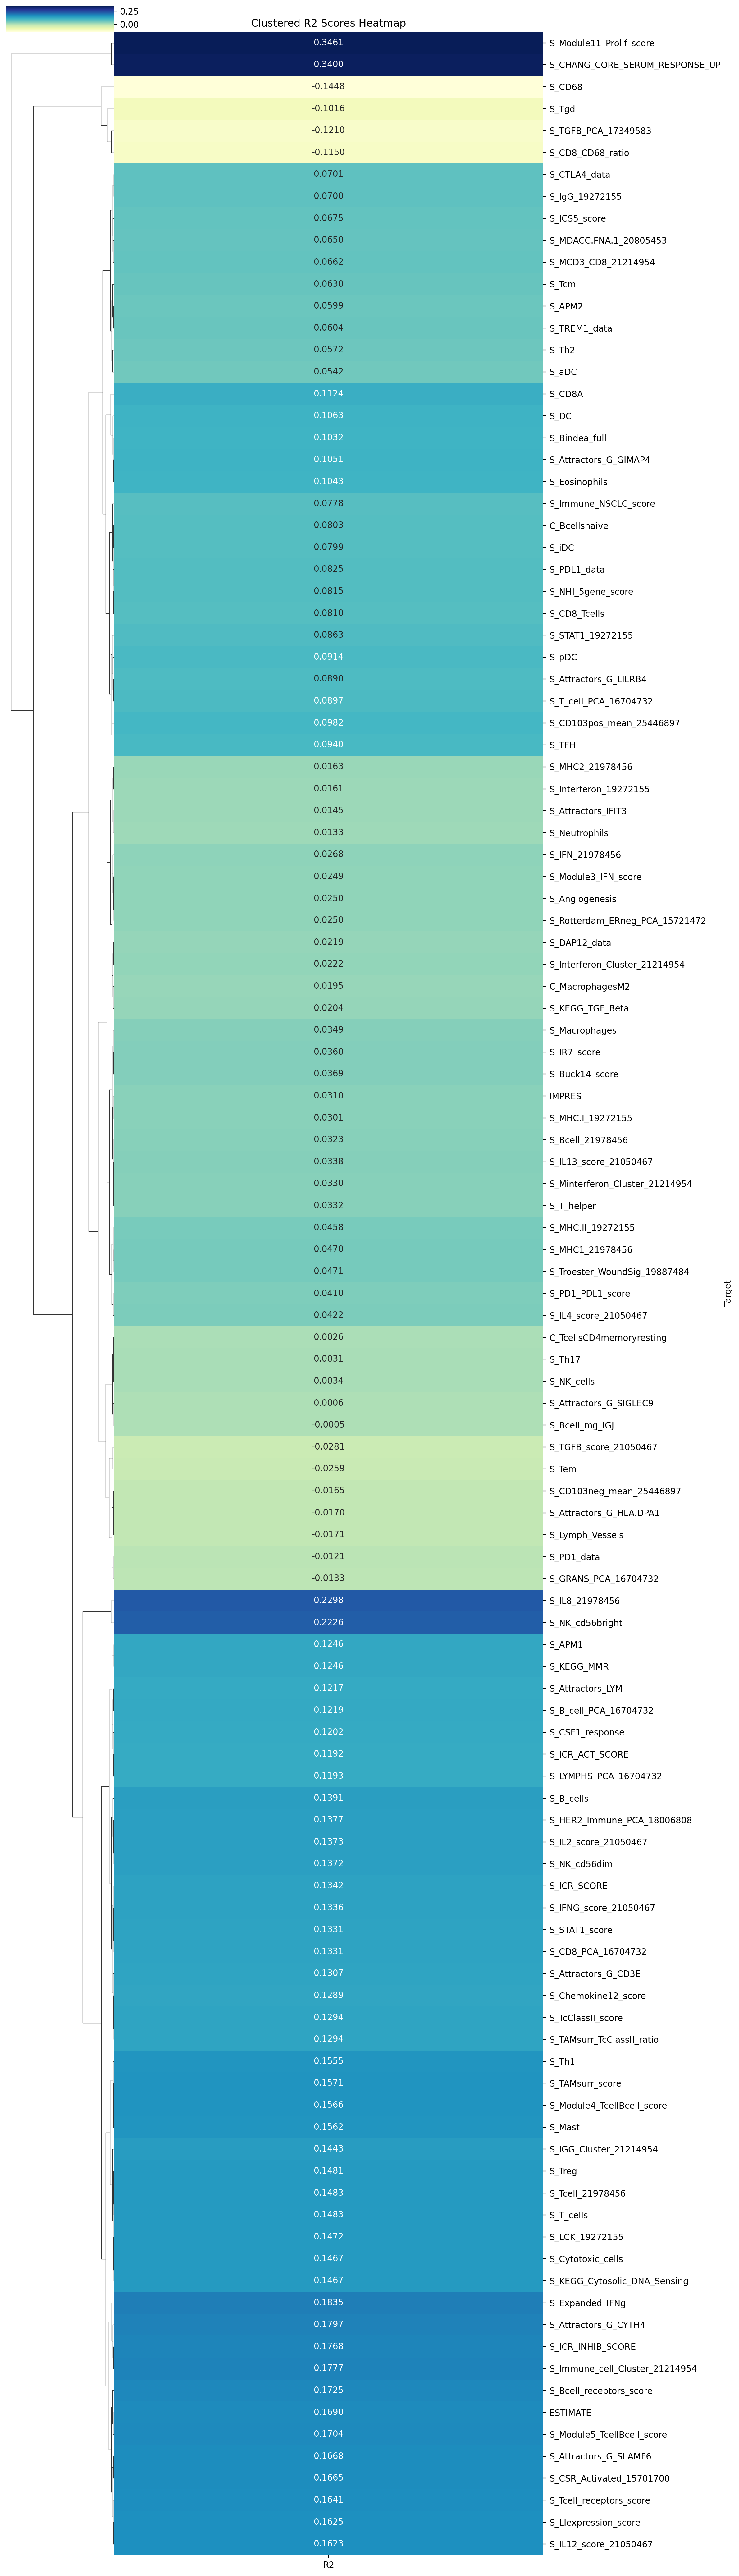
\includegraphics[width=12.38542in,height=43.17708in]{xgboost_tuned_files/figure-pdf/cell-45-output-1.png}

\begin{Shaded}
\begin{Highlighting}[]
\CommentTok{\# use the predefined lists of immune score subgroups}
\CommentTok{\# Extract R2 scores into a DataFrame}
\NormalTok{r2\_data }\OperatorTok{=}\NormalTok{ \{target: metrics.test\_r2 }\ControlFlowTok{for}\NormalTok{ target, metrics }\KeywordTok{in}\NormalTok{ tuned\_results.items()\}}
\NormalTok{df\_r2 }\OperatorTok{=}\NormalTok{ pd.DataFrame(}\BuiltInTok{list}\NormalTok{(r2\_data.items()), columns}\OperatorTok{=}\NormalTok{[}\StringTok{\textquotesingle{}Target\textquotesingle{}}\NormalTok{, }\StringTok{\textquotesingle{}R2\textquotesingle{}}\NormalTok{])}

\CommentTok{\# Add a \textquotesingle{}Group\textquotesingle{} column based on the predefined groups}
\NormalTok{df\_r2[}\StringTok{\textquotesingle{}Group\textquotesingle{}}\NormalTok{] }\OperatorTok{=}\NormalTok{ df\_r2[}\StringTok{\textquotesingle{}Target\textquotesingle{}}\NormalTok{].}\BuiltInTok{apply}\NormalTok{(}\KeywordTok{lambda}\NormalTok{ x: }\BuiltInTok{next}\NormalTok{((k }\ControlFlowTok{for}\NormalTok{ k, v }\KeywordTok{in}\NormalTok{ imscore\_series\_dict.items() }\ControlFlowTok{if}\NormalTok{ x }\KeywordTok{in}\NormalTok{ v), }\StringTok{\textquotesingle{}Other\textquotesingle{}}\NormalTok{))}

\CommentTok{\# Sort the DataFrame by group and then by R2 score within each group}
\NormalTok{df\_r2 }\OperatorTok{=}\NormalTok{ df\_r2.sort\_values([}\StringTok{\textquotesingle{}Group\textquotesingle{}}\NormalTok{, }\StringTok{\textquotesingle{}R2\textquotesingle{}}\NormalTok{], ascending}\OperatorTok{=}\NormalTok{[}\VariableTok{True}\NormalTok{, }\VariableTok{False}\NormalTok{])}
\NormalTok{df\_r2 }\OperatorTok{=}\NormalTok{ df\_r2.reset\_index(drop}\OperatorTok{=}\VariableTok{True}\NormalTok{)}

\CommentTok{\# Create a color palette for the groups}
\NormalTok{palette }\OperatorTok{=}\NormalTok{ sns.color\_palette(}\StringTok{"husl"}\NormalTok{, }\BuiltInTok{len}\NormalTok{(imscore\_series\_dict))}
\NormalTok{group\_colors }\OperatorTok{=} \BuiltInTok{dict}\NormalTok{(}\BuiltInTok{zip}\NormalTok{(imscore\_series\_dict.keys(), palette))}

\CommentTok{\# Create the plot}
\NormalTok{plt.figure(figsize}\OperatorTok{=}\NormalTok{(}\DecValTok{12}\NormalTok{, }\BuiltInTok{len}\NormalTok{(df\_r2) }\OperatorTok{*} \FloatTok{0.4} \OperatorTok{+} \DecValTok{2}\NormalTok{))}

\CommentTok{\# Plot the heatmap}
\NormalTok{sns.heatmap(df\_r2.set\_index(}\StringTok{\textquotesingle{}Target\textquotesingle{}}\NormalTok{)[[}\StringTok{\textquotesingle{}R2\textquotesingle{}}\NormalTok{]], }
\NormalTok{            cmap}\OperatorTok{=}\StringTok{\textquotesingle{}YlGnBu\textquotesingle{}}\NormalTok{, }
\NormalTok{            annot}\OperatorTok{=}\VariableTok{True}\NormalTok{, }
\NormalTok{            fmt}\OperatorTok{=}\StringTok{\textquotesingle{}.4f\textquotesingle{}}\NormalTok{, }
\NormalTok{            cbar\_kws}\OperatorTok{=}\NormalTok{\{}\StringTok{\textquotesingle{}label\textquotesingle{}}\NormalTok{: }\StringTok{\textquotesingle{}R2 Score\textquotesingle{}}\NormalTok{\})}

\CommentTok{\# Add colored bars to indicate groups}
\ControlFlowTok{for}\NormalTok{ i, (idx, row) }\KeywordTok{in} \BuiltInTok{enumerate}\NormalTok{(df\_r2.iterrows()):}
\NormalTok{    plt.annotate(}\StringTok{\textquotesingle{}\textquotesingle{}}\NormalTok{, xy}\OperatorTok{=}\NormalTok{(}\OperatorTok{{-}}\FloatTok{0.1}\NormalTok{, i), xytext}\OperatorTok{=}\NormalTok{(}\OperatorTok{{-}}\FloatTok{0.5}\NormalTok{, i),}
\NormalTok{                 arrowprops}\OperatorTok{=}\BuiltInTok{dict}\NormalTok{(arrowstyle}\OperatorTok{=}\StringTok{\textquotesingle{}{-}\textquotesingle{}}\NormalTok{, color}\OperatorTok{=}\NormalTok{group\_colors.get(row[}\StringTok{\textquotesingle{}Group\textquotesingle{}}\NormalTok{], }\StringTok{\textquotesingle{}gray\textquotesingle{}}\NormalTok{),}
\NormalTok{                                 lw}\OperatorTok{=}\DecValTok{5}\NormalTok{),}
\NormalTok{                 va}\OperatorTok{=}\StringTok{\textquotesingle{}center\textquotesingle{}}\NormalTok{)}

\CommentTok{\# Customize the plot}
\NormalTok{plt.title(}\StringTok{\textquotesingle{}R2 Scores Grouped by Target Categories\textquotesingle{}}\NormalTok{, pad}\OperatorTok{=}\DecValTok{20}\NormalTok{)}
\NormalTok{plt.ylabel(}\StringTok{\textquotesingle{}Targets\textquotesingle{}}\NormalTok{)}
\NormalTok{plt.xticks([])  }\CommentTok{\# Remove x{-}axis labels as they\textquotesingle{}re redundant}
\NormalTok{plt.tick\_params(axis}\OperatorTok{=}\StringTok{\textquotesingle{}y\textquotesingle{}}\NormalTok{, which}\OperatorTok{=}\StringTok{\textquotesingle{}major\textquotesingle{}}\NormalTok{, labelsize}\OperatorTok{=}\DecValTok{8}\NormalTok{, rotation}\OperatorTok{=}\DecValTok{0}\NormalTok{)}

\CommentTok{\# Add a legend for groups}
\NormalTok{handles }\OperatorTok{=}\NormalTok{ [plt.Rectangle((}\DecValTok{0}\NormalTok{,}\DecValTok{0}\NormalTok{),}\DecValTok{1}\NormalTok{,}\DecValTok{1}\NormalTok{, color}\OperatorTok{=}\NormalTok{group\_colors[group]) }\ControlFlowTok{for}\NormalTok{ group }\KeywordTok{in}\NormalTok{ imscore\_series\_dict.keys()]}
\NormalTok{plt.legend(handles, imscore\_series\_dict.keys(), title}\OperatorTok{=}\StringTok{\textquotesingle{}Target Groups\textquotesingle{}}\NormalTok{, }
\NormalTok{           bbox\_to\_anchor}\OperatorTok{=}\NormalTok{(}\FloatTok{1.05}\NormalTok{, }\DecValTok{1}\NormalTok{), loc}\OperatorTok{=}\StringTok{\textquotesingle{}upper left\textquotesingle{}}\NormalTok{)}

\NormalTok{plt.tight\_layout()}
\NormalTok{plt.show()}
\end{Highlighting}
\end{Shaded}

\begin{verbatim}
{'HR>1': ['S_TREM1_data', 'S_CHANG_CORE_SERUM_RESPONSE_UP', 'S_IL8_21978456'], 'HR>1_worst_10_prog': ['S_TGFB_score_21050467', 'S_TGFB_PCA_17349583', 'S_Lymph_Vessels', 'S_Rotterdam_ERneg_PCA_15721472', 'S_IFNG_score_21050467', 'S_Module11_Prolif_score', 'S_TREM1_data'], 'HR<1': ['S_Buck14_score', 'S_Bcell_receptors_score', 'S_TFH', 'S_CD103pos_mean_25446897', 'S_T_helper'], 'HR<1_best_10_prog': ['S_Buck14_score', 'S_Bcell_receptors_score', 'S_TFH', 'S_CD103pos_mean_25446897', 'S_T_helper', 'S_Attractors_G_SLAMF6', 'S_ICS5_score'], 'cytokine_chemokine_activator': ['S_Expanded_IFNg', 'S_IL2_score_21050467', 'S_IL12_score_21050467', 'S_IFNG_score_21050467', 'S_IR7_score', 'S_Interferon_19272155', 'S_Minterferon_Cluster_21214954', 'S_Interferon_Cluster_21214954', 'S_IFN_21978456', 'S_Attractors_IFIT3', 'S_Module3_IFN_score'], 'activator_T': ['S_T_cells', 'S_Tcell_receptors_score', 'S_Tcell_21978456', 'S_CD8_Tcells', 'S_CD8A', 'S_T_helper', 'S_Th17', 'S_Tcm', 'S_Tem', 'S_Th1', 'S_TFH', 'S_Cytotoxic_cells', 'C_TcellsCD4memoryresting', 'S_T_cell_PCA_16704732', 'S_Attractors_G_CD3E', 'S_Tgd', 'S_CD8_PCA_16704732', 'S_Module4_TcellBcell_score', 'S_Module5_TcellBcell_score', 'S_CD8_CD68_ratio', 'S_ICR_SCORE', 'S_ICR_ACT_SCORE', 'S_GRANS_PCA_16704732'], 'suppressor_T': ['S_Treg', 'S_TGFB_score_21050467', 'S_CTLA4_data', 'S_PD1_data', 'S_PDL1_data', 'S_PD1_PDL1_score', 'S_IL4_score_21050467', 'S_IL13_score_21050467', 'S_TGFB_PCA_17349583', 'S_TcClassII_score', 'S_KEGG_TGF_Beta', 'S_ICR_INHIB_SCORE'], 'B_cell_all': ['S_CSR_Activated_15701700', 'S_Bcell_receptors_score', 'S_B_cell_PCA_16704732'], 'innate_cell_all': ['S_pDC'], 'general': ['S_Buck14_score', 'S_Rotterdam_ERneg_PCA_15721472', 'S_KEGG_Cytosolic_DNA_Sensing']}
\end{verbatim}

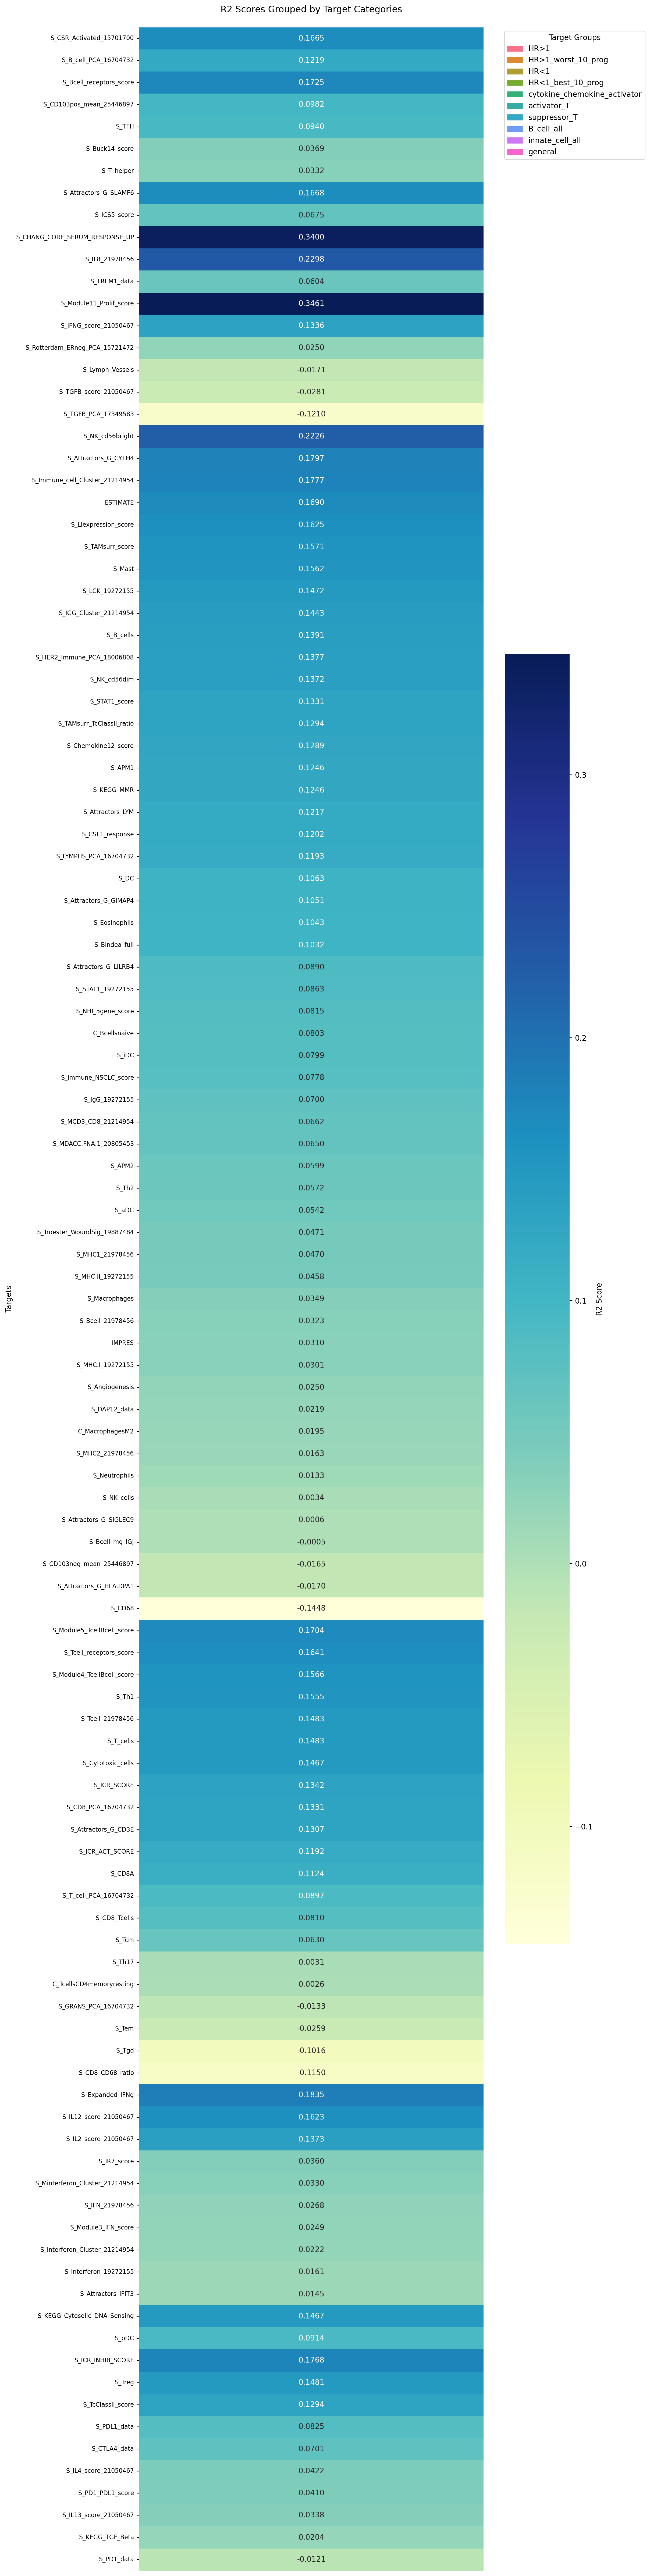
\includegraphics[width=12.58333in,height=49.90625in]{xgboost_tuned_files/figure-pdf/cell-46-output-2.png}

\begin{Shaded}
\begin{Highlighting}[]
\ImportTok{from}\NormalTok{ matplotlib.colors }\ImportTok{import}\NormalTok{ LinearSegmentedColormap}

\CommentTok{\# Extract R2 scores into a DataFrame}
\NormalTok{r2\_data }\OperatorTok{=}\NormalTok{ \{target: metrics.test\_r2 }\ControlFlowTok{for}\NormalTok{ target, metrics }\KeywordTok{in}\NormalTok{ tuned\_results.items()\}}
\NormalTok{df\_r2 }\OperatorTok{=}\NormalTok{ pd.DataFrame(}\BuiltInTok{list}\NormalTok{(r2\_data.items()), columns}\OperatorTok{=}\NormalTok{[}\StringTok{\textquotesingle{}Target\textquotesingle{}}\NormalTok{, }\StringTok{\textquotesingle{}R2\textquotesingle{}}\NormalTok{])}

\CommentTok{\# Add a \textquotesingle{}Group\textquotesingle{} column based on the predefined groups}
\NormalTok{df\_r2[}\StringTok{\textquotesingle{}Group\textquotesingle{}}\NormalTok{] }\OperatorTok{=}\NormalTok{ df\_r2[}\StringTok{\textquotesingle{}Target\textquotesingle{}}\NormalTok{].}\BuiltInTok{apply}\NormalTok{(}\KeywordTok{lambda}\NormalTok{ x: }\BuiltInTok{next}\NormalTok{((k }\ControlFlowTok{for}\NormalTok{ k, v }\KeywordTok{in}\NormalTok{ imscore\_series\_dict.items() }\ControlFlowTok{if}\NormalTok{ x }\KeywordTok{in}\NormalTok{ v), }\StringTok{\textquotesingle{}Other\textquotesingle{}}\NormalTok{))}

\CommentTok{\# Sort the DataFrame by group and then by R2 score within each group}
\NormalTok{df\_r2 }\OperatorTok{=}\NormalTok{ df\_r2.sort\_values([}\StringTok{\textquotesingle{}Group\textquotesingle{}}\NormalTok{, }\StringTok{\textquotesingle{}R2\textquotesingle{}}\NormalTok{], ascending}\OperatorTok{=}\NormalTok{[}\VariableTok{True}\NormalTok{, }\VariableTok{False}\NormalTok{])}

\NormalTok{springpastel }\OperatorTok{=}\NormalTok{ [}\StringTok{"\#fd7f6f"}\NormalTok{, }\StringTok{"\#7eb0d5"}\NormalTok{, }\StringTok{"\#b2e061"}\NormalTok{, }\StringTok{"\#bd7ebe"}\NormalTok{, }\StringTok{"\#ffb55a"}\NormalTok{, }\StringTok{"\#ebdc78"}\NormalTok{, }\StringTok{"\#beb9db"}\NormalTok{, }\StringTok{"\#fdcce5"}\NormalTok{, }\StringTok{"\#8bd3c7"}\NormalTok{, }\StringTok{"\#7c1158"}\NormalTok{]}

\CommentTok{\# Create a color palette for the groups}
\NormalTok{palette }\OperatorTok{=}\NormalTok{ sns.color\_palette(springpastel, }\BuiltInTok{len}\NormalTok{(imscore\_series\_dict))}
\NormalTok{group\_colors }\OperatorTok{=} \BuiltInTok{dict}\NormalTok{(}\BuiltInTok{zip}\NormalTok{(imscore\_series\_dict.keys(), palette))}

\CommentTok{\# Create the plot}
\NormalTok{plt.figure(figsize}\OperatorTok{=}\NormalTok{(}\DecValTok{14}\NormalTok{, }\BuiltInTok{len}\NormalTok{(df\_r2) }\OperatorTok{*} \FloatTok{0.2} \OperatorTok{+} \DecValTok{2}\NormalTok{))}

\CommentTok{\# Create a custom colormap for the heatmap}
\NormalTok{cmap }\OperatorTok{=}\NormalTok{ LinearSegmentedColormap.from\_list(}\StringTok{"custom"}\NormalTok{, [}\StringTok{"\#FFFFFF"}\NormalTok{, }\StringTok{"\#4a4a4a"}\NormalTok{])}

\CommentTok{\# Plot the heatmap}
\NormalTok{sns.heatmap(df\_r2.set\_index(}\StringTok{\textquotesingle{}Target\textquotesingle{}}\NormalTok{)[[}\StringTok{\textquotesingle{}R2\textquotesingle{}}\NormalTok{]], cmap}\OperatorTok{=}\NormalTok{cmap, annot}\OperatorTok{=}\VariableTok{True}\NormalTok{, fmt}\OperatorTok{=}\StringTok{\textquotesingle{}.4f\textquotesingle{}}\NormalTok{, cbar}\OperatorTok{=}\VariableTok{False}\NormalTok{)}

\CommentTok{\# Color the y{-}axis labels based on their group}
\NormalTok{ax }\OperatorTok{=}\NormalTok{ plt.gca()}
\ControlFlowTok{for}\NormalTok{ i, (idx, row) }\KeywordTok{in} \BuiltInTok{enumerate}\NormalTok{(df\_r2.iterrows()):}
\NormalTok{    ax.get\_yticklabels()[i].set\_color(group\_colors.get(row[}\StringTok{\textquotesingle{}Group\textquotesingle{}}\NormalTok{], }\StringTok{\textquotesingle{}gray\textquotesingle{}}\NormalTok{))}
\NormalTok{    ax.get\_yticklabels()[i].set\_fontweight(}\StringTok{\textquotesingle{}bold\textquotesingle{}}\NormalTok{)  }\CommentTok{\# Make labels bold for better readability}

\CommentTok{\# Customize the plot}
\NormalTok{plt.title(}\StringTok{\textquotesingle{}R2 Scores Across Immune Score Subgroups\textquotesingle{}}\NormalTok{, pad}\OperatorTok{=}\DecValTok{20}\NormalTok{)}
\NormalTok{plt.ylabel(}\StringTok{\textquotesingle{}Immune Score Subgroups\textquotesingle{}}\NormalTok{)}
\NormalTok{plt.xticks([])  }\CommentTok{\# Remove x{-}axis labels as they\textquotesingle{}re redundant}
\NormalTok{plt.tick\_params(axis}\OperatorTok{=}\StringTok{\textquotesingle{}y\textquotesingle{}}\NormalTok{, which}\OperatorTok{=}\StringTok{\textquotesingle{}major\textquotesingle{}}\NormalTok{, labelsize}\OperatorTok{=}\DecValTok{8}\NormalTok{, rotation}\OperatorTok{=}\DecValTok{0}\NormalTok{)}

\CommentTok{\# Add a legend for groups}
\NormalTok{handles }\OperatorTok{=}\NormalTok{ [plt.Rectangle((}\DecValTok{0}\NormalTok{,}\DecValTok{0}\NormalTok{),}\DecValTok{1}\NormalTok{,}\DecValTok{1}\NormalTok{, color}\OperatorTok{=}\NormalTok{group\_colors[group]) }\ControlFlowTok{for}\NormalTok{ group }\KeywordTok{in}\NormalTok{ imscore\_series\_dict.keys()]}
\NormalTok{plt.legend(handles, imscore\_series\_dict.keys(), title}\OperatorTok{=}\StringTok{\textquotesingle{}Immune Score Subgroups\textquotesingle{}}\NormalTok{, bbox\_to\_anchor}\OperatorTok{=}\NormalTok{(}\FloatTok{1.05}\NormalTok{, }\DecValTok{1}\NormalTok{), loc}\OperatorTok{=}\StringTok{\textquotesingle{}upper left\textquotesingle{}}\NormalTok{)}

\NormalTok{plt.tight\_layout()}
\NormalTok{plt.show()}
\end{Highlighting}
\end{Shaded}

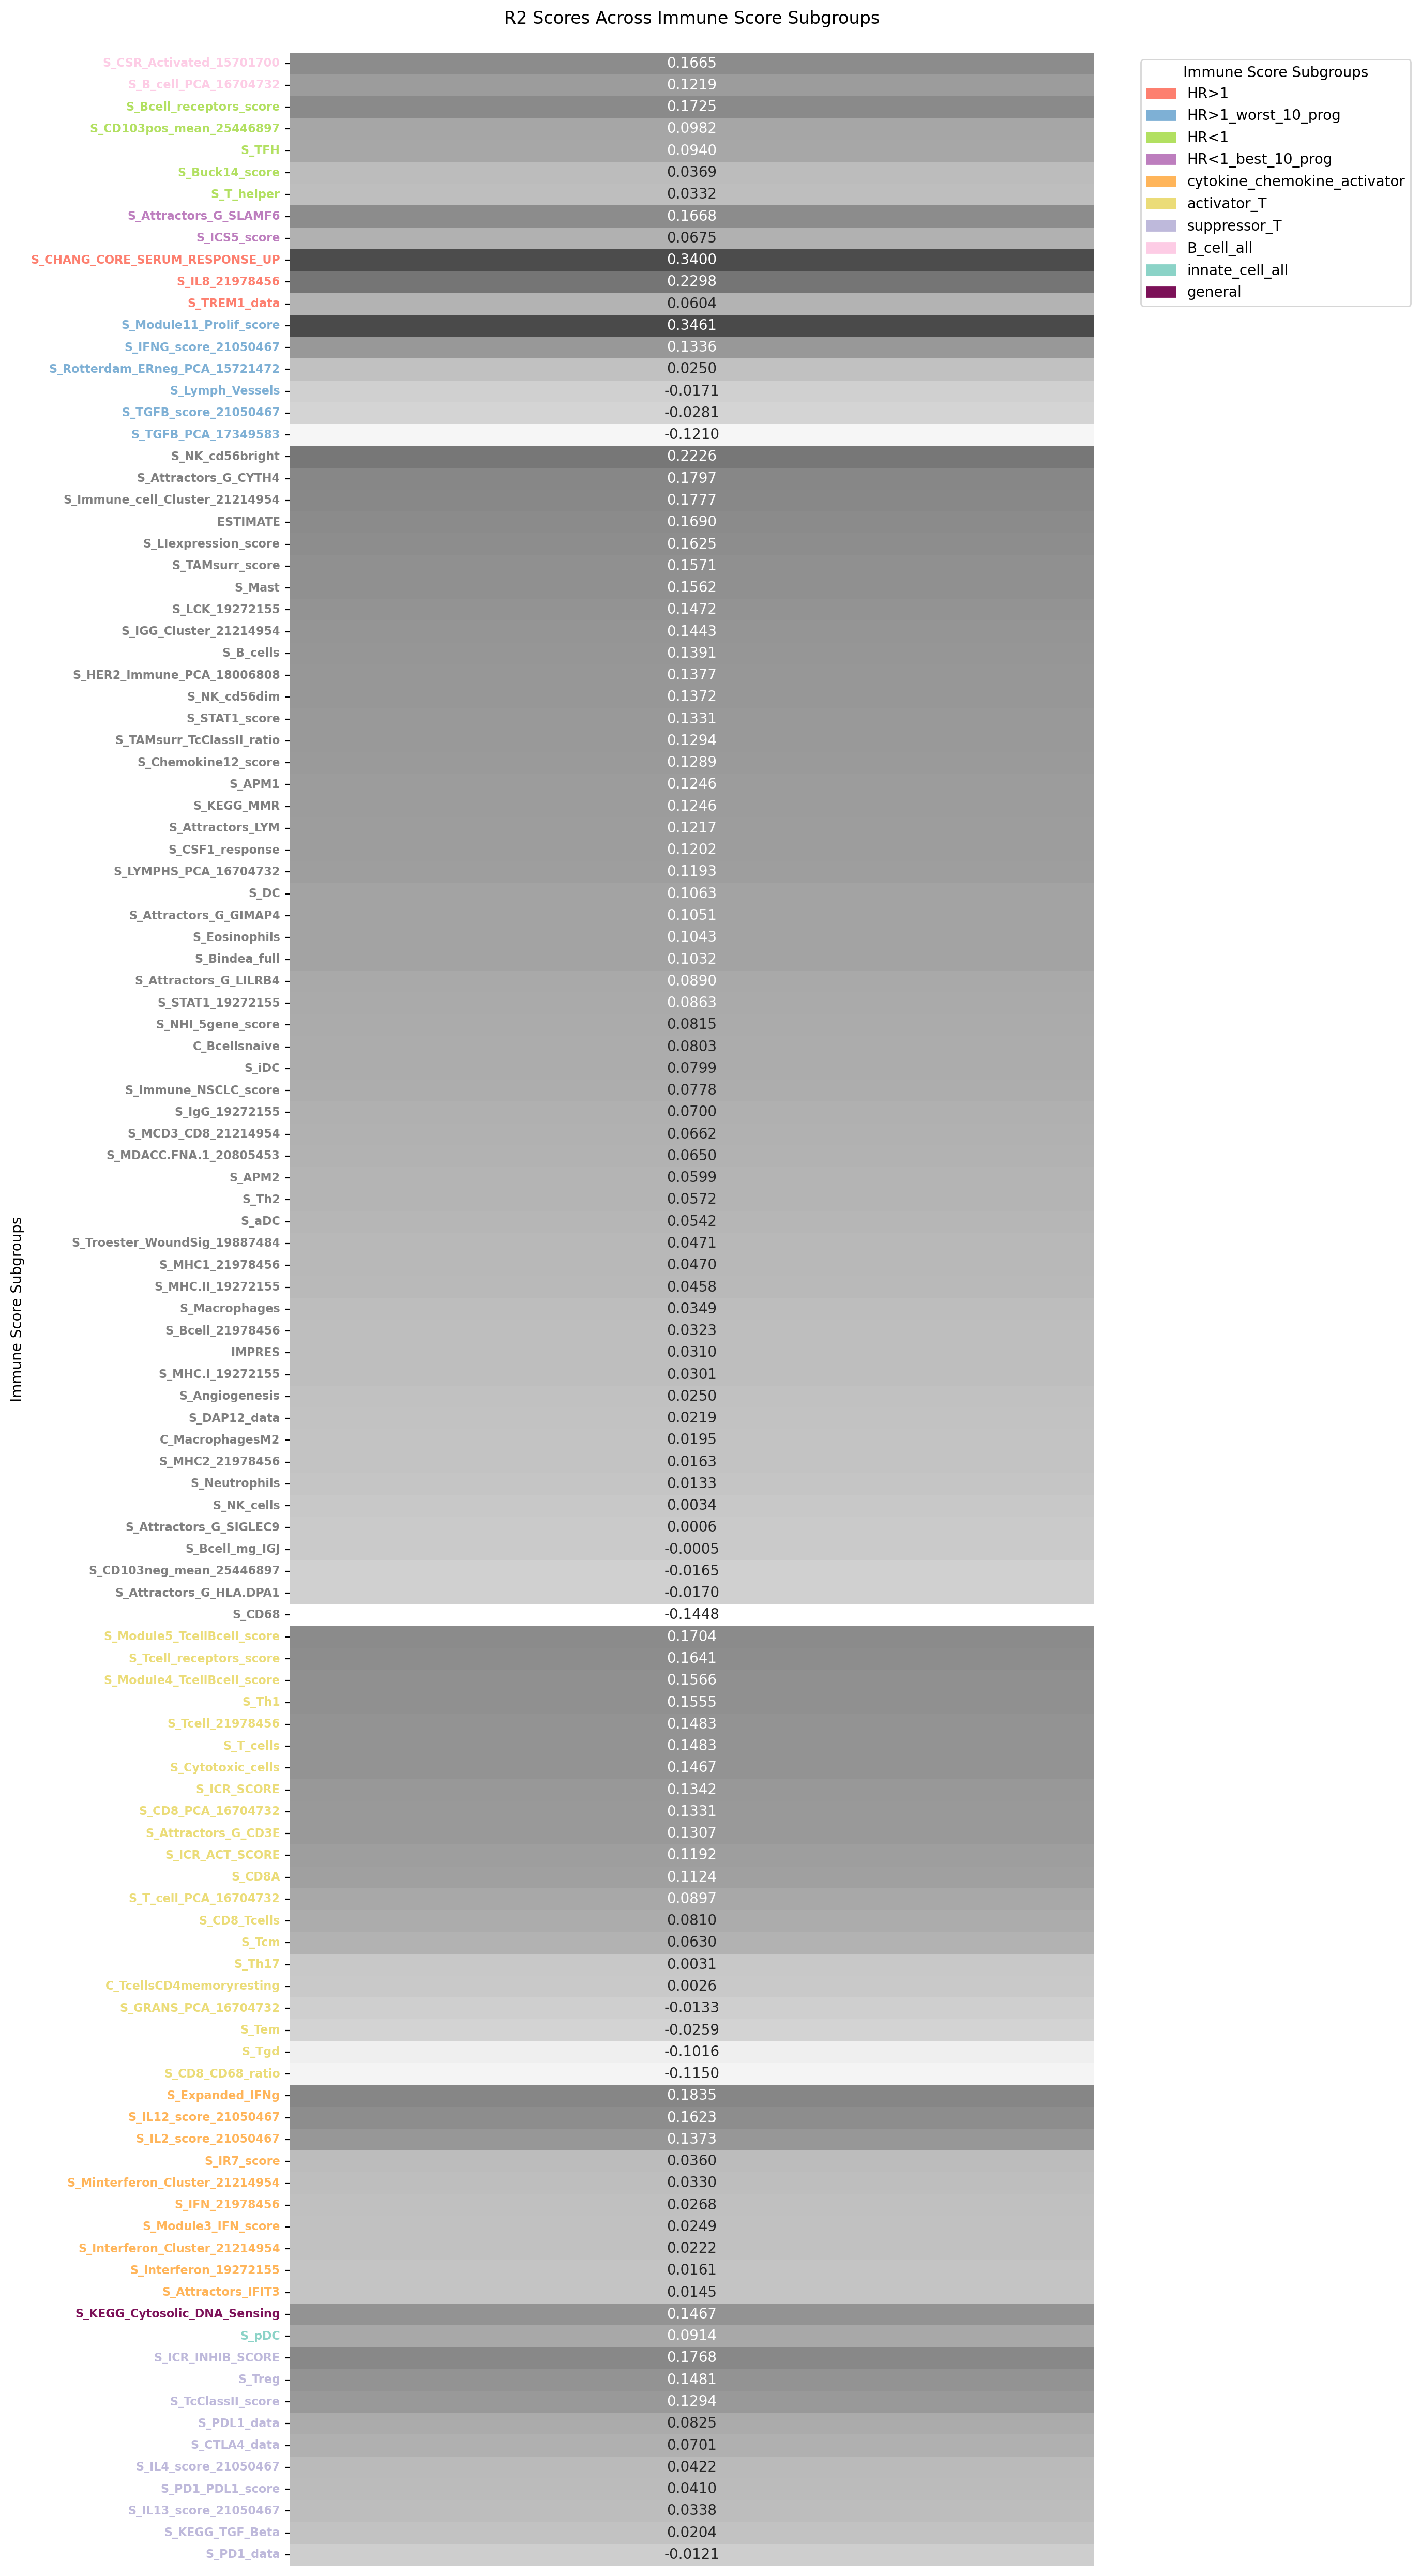
\includegraphics[width=14.3125in,height=25.94792in]{xgboost_tuned_files/figure-pdf/cell-47-output-1.png}

\begin{Shaded}
\begin{Highlighting}[]
\CommentTok{\# Create a faceted bar plot}
\NormalTok{g }\OperatorTok{=}\NormalTok{ sns.FacetGrid(df\_r2, col}\OperatorTok{=}\StringTok{"Group"}\NormalTok{, col\_wrap}\OperatorTok{=}\DecValTok{2}\NormalTok{, height}\OperatorTok{=}\DecValTok{4}\NormalTok{, aspect}\OperatorTok{=}\FloatTok{1.5}\NormalTok{)}
\NormalTok{g.}\BuiltInTok{map}\NormalTok{(sns.barplot, }\StringTok{"Target"}\NormalTok{, }\StringTok{"R2"}\NormalTok{, order}\OperatorTok{=}\NormalTok{df\_r2.sort\_values(}\StringTok{\textquotesingle{}R2\textquotesingle{}}\NormalTok{, ascending}\OperatorTok{=}\VariableTok{False}\NormalTok{)[}\StringTok{\textquotesingle{}Target\textquotesingle{}}\NormalTok{])}
\NormalTok{g.set\_xticklabels(rotation}\OperatorTok{=}\DecValTok{90}\NormalTok{)}
\NormalTok{g.set\_axis\_labels(}\StringTok{""}\NormalTok{, }\StringTok{"R2 Score"}\NormalTok{)}
\NormalTok{g.figure.suptitle(}\StringTok{"R2 Scores by Immune Subgroups"}\NormalTok{, y}\OperatorTok{=}\FloatTok{1.02}\NormalTok{)}
\NormalTok{g.tight\_layout()}
\NormalTok{plt.show()}
\end{Highlighting}
\end{Shaded}

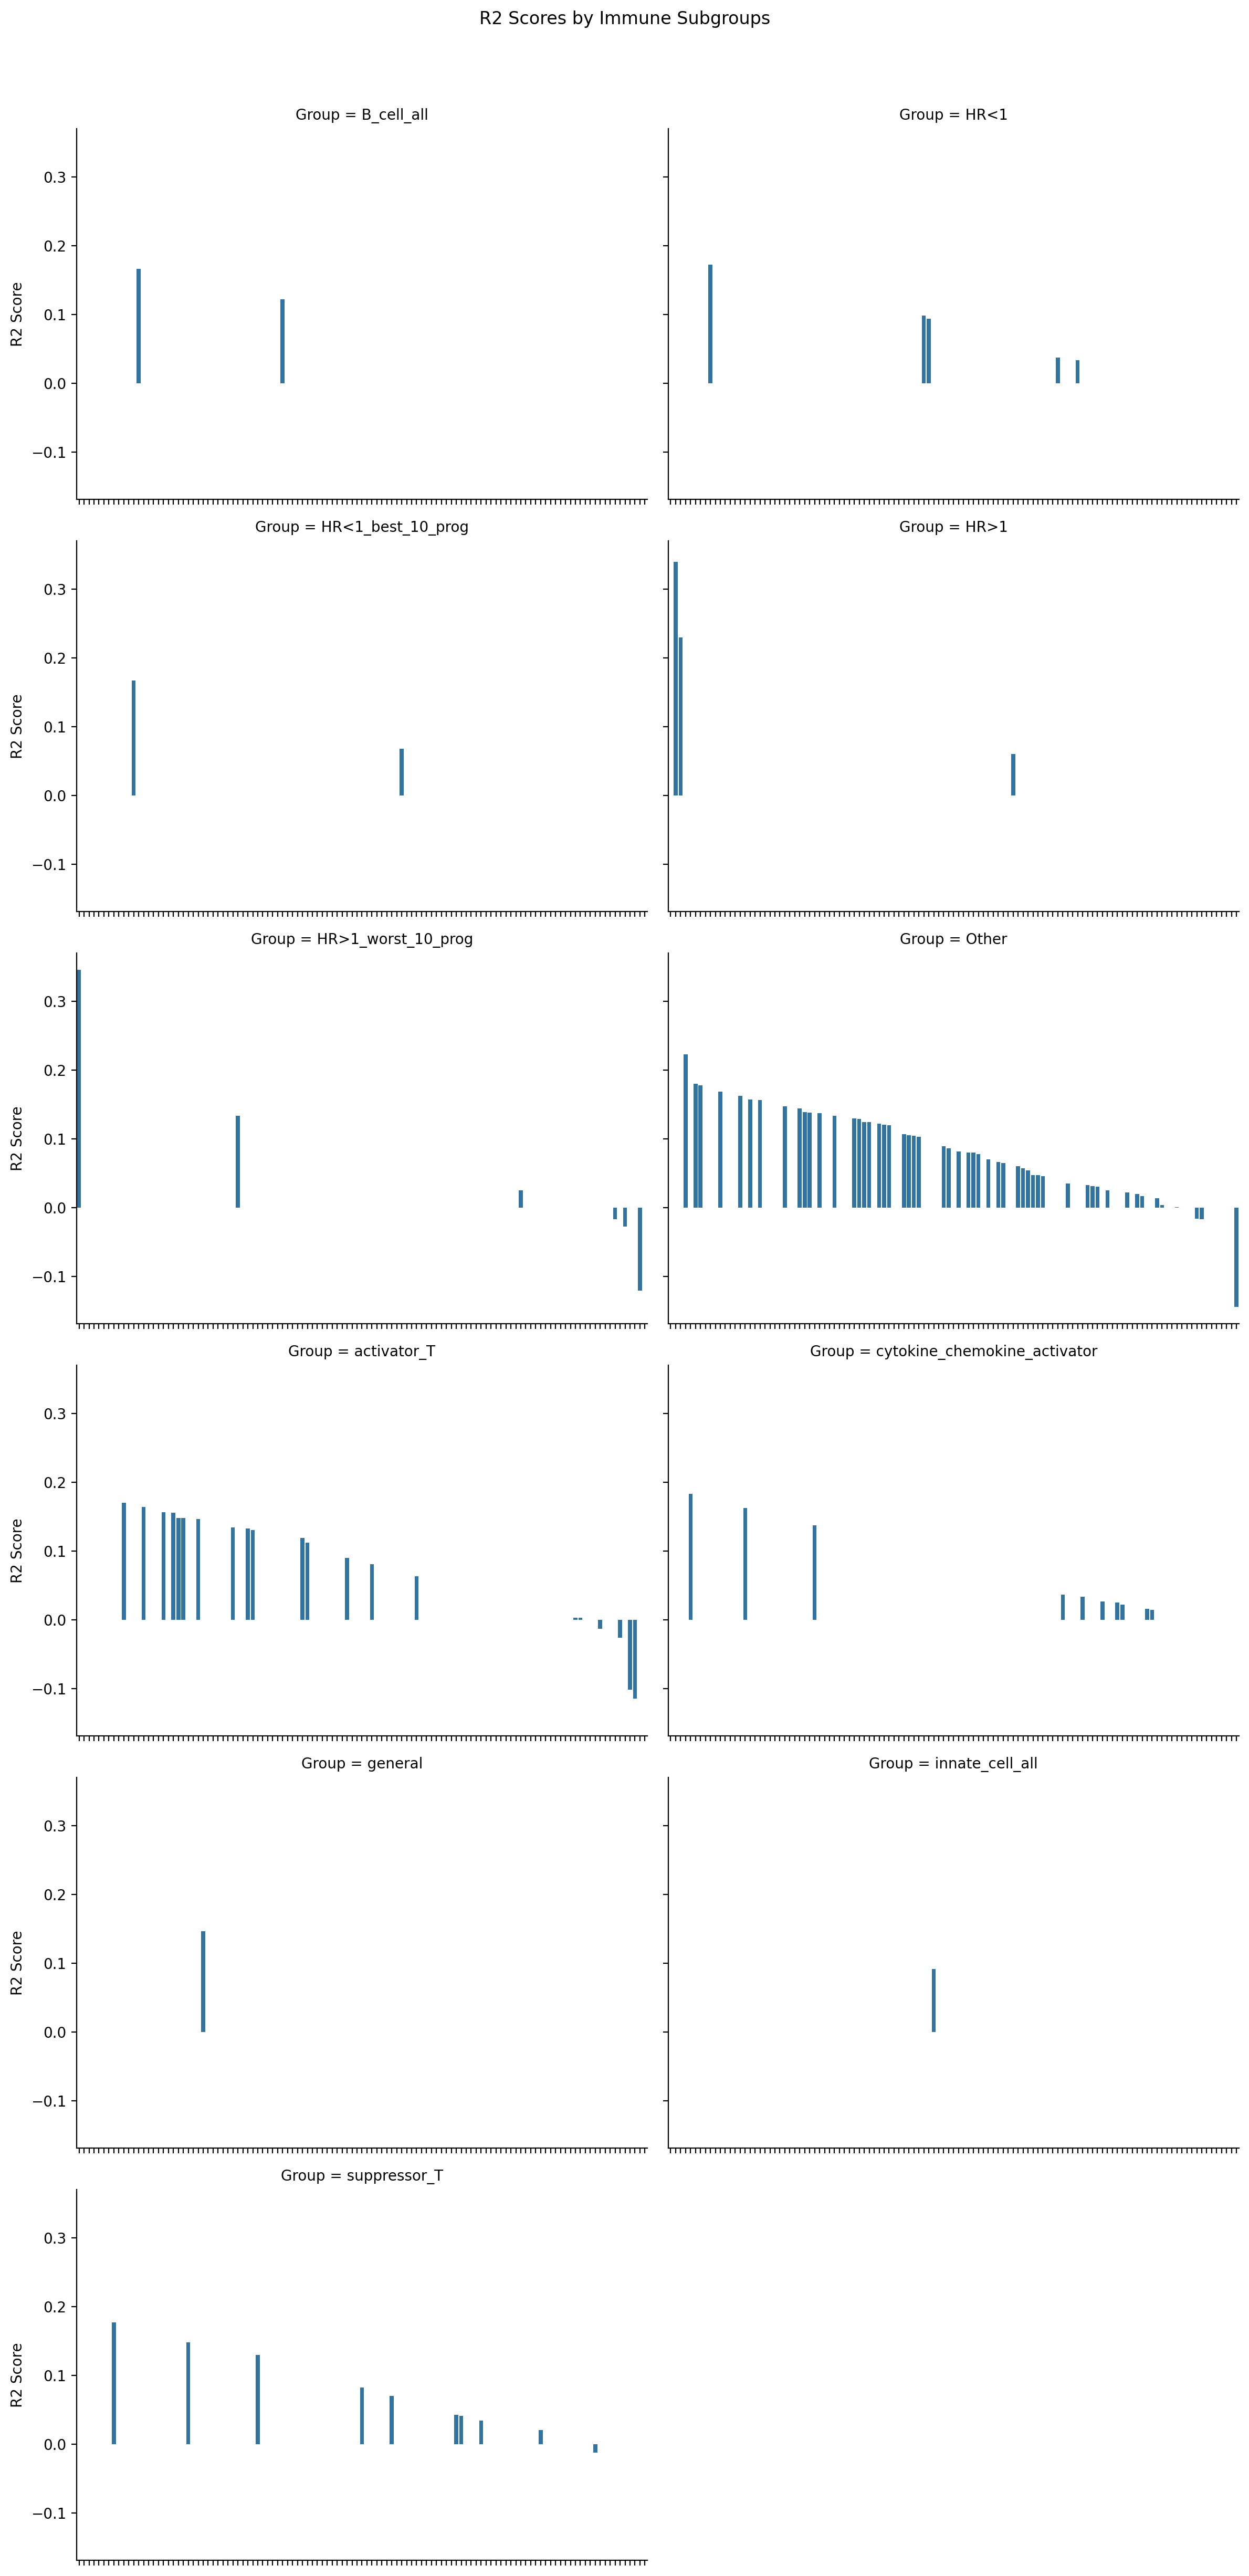
\includegraphics[width=12.38542in,height=25.55208in]{xgboost_tuned_files/figure-pdf/cell-48-output-1.png}

\paragraph{\texorpdfstring{\textbf{Conclusion}}{Conclusion}}\label{conclusion}

Maybe XGBoost could not capture the weak nonlinear interactions between
chosen X features and the immune scores despite hyperparameter tuning
and cross-validation.

What's next?

\begin{enumerate}
\def\labelenumi{\arabic{enumi}.}
\tightlist
\item
  Support Vector Regressor might fare better (with CV)
\item
  X features might not be informative enough. Worth considering adding
  other variables? Survival? Response to treatment?
\item
  This also implies that maybe the question needs to be reframed into a
  classification task?
\end{enumerate}




\end{document}
